\documentclass[12pt]{article}
\usepackage[english]{babel}
\usepackage[utf8x]{inputenc}
\usepackage[font=small,labelfont=bf]{caption}
\usepackage{amsmath}
\usepackage{graphicx}
\usepackage[colorinlistoftodos]{todonotes}
\usepackage{tabularx} % in the preamble

\begin{document}
	
	\begin{titlepage}
		
		\newcommand{\HRule}{\rule{\linewidth}{0.5mm}} % Defines a new command for the horizontal lines, change thickness here
		
		\center % Center everything on the page
		
		%----------------------------------------------------------------------------------------
		%	HEADING SECTIONS
		%----------------------------------------------------------------------------------------
		
		\textsc{\LARGE Central Washington University}\\[1.5cm] % Name of your university/college
		\textsc{\Large CS 471 OPTIMIZATION}\\[0.5cm] % Major heading such as course name
		\textsc{\large Spring 2019}\\[0.5cm] % Minor heading such as course title
		
		%----------------------------------------------------------------------------------------
		%	TITLE SECTION
		%----------------------------------------------------------------------------------------
		
		\HRule \\[0.4cm]
		{ \huge \bfseries Project 5 Report}\\[0.4cm] % Title of your document
		\HRule \\[1.5cm]
		
		%----------------------------------------------------------------------------------------
		%	AUTHOR SECTION
		%----------------------------------------------------------------------------------------
		
		\begin{minipage}{0.4\textwidth}
			\begin{flushleft} \large
				\emph{Author:}\\
				Hermann \textsc{Yepdjio} % Your name
			\end{flushleft}
		\end{minipage}
		~
		\begin{minipage}{0.4\textwidth}
			\begin{flushright} \large
				\emph{Supervisor:} \\
				Dr. Donald \textsc{Davendra} % Supervisor's Name
			\end{flushright}
		\end{minipage}\\[1cm]
		
		% If you don't want a supervisor, uncomment the two lines below and remove the section above
		%\Large \emph{Author:}\\
		%John \textsc{Smith}\\[3cm] % Your name
		
		%----------------------------------------------------------------------------------------
		%	DATE SECTION
		%----------------------------------------------------------------------------------------
		
		{\large \today}\\ % Date, change the \today to a set date if you want to be precise
		
		%----------------------------------------------------------------------------------------
		%	LOGO SECTION
		%----------------------------------------------------------------------------------------
		
		
\includegraphics[width=12cm]{CWU-Logo.png}\\[.5cm] % Include a department/university logo - this will require the graphicx package
		
		%----------------------------------------------------------------------------------------
		
		\vfill % Fill the rest of the page with whitespace
		
	\end{titlepage}
	\newpage
	\tableofcontents
	\newpage
	
	
	
	\section{Introduction}
	Project 5 was about optimizing 3 standard job scheduling functions namely, Flow Shop Scheduling (FSS), Flow Shop Scheduling with Blocking(FSSB) and Flow Shop Scheduling with No Wait (FSSNW). For this purpose, one optimization algorithm was to be implemented then applied to those functions. The algorithm is called NEH (Nawaz Enscore Ham) heuristic. After being implemented, the it was run on each of the 3 functions using as input, some data that was provided along with the project in the form of text files. Important details were recorded during the experimentation process then stored in a tabular format and they will be discussed then analyzed later on in this report. However, in order to visually observe how the jobs should be scheduled according to the NEH heuristic, Gantt charts were generated for some of the results and they are also discussed later on in this report.
	
		
	\section{Results}
		\subsection{Flow Shop Scheduling}
			\subsubsection{Gantt Charts}
				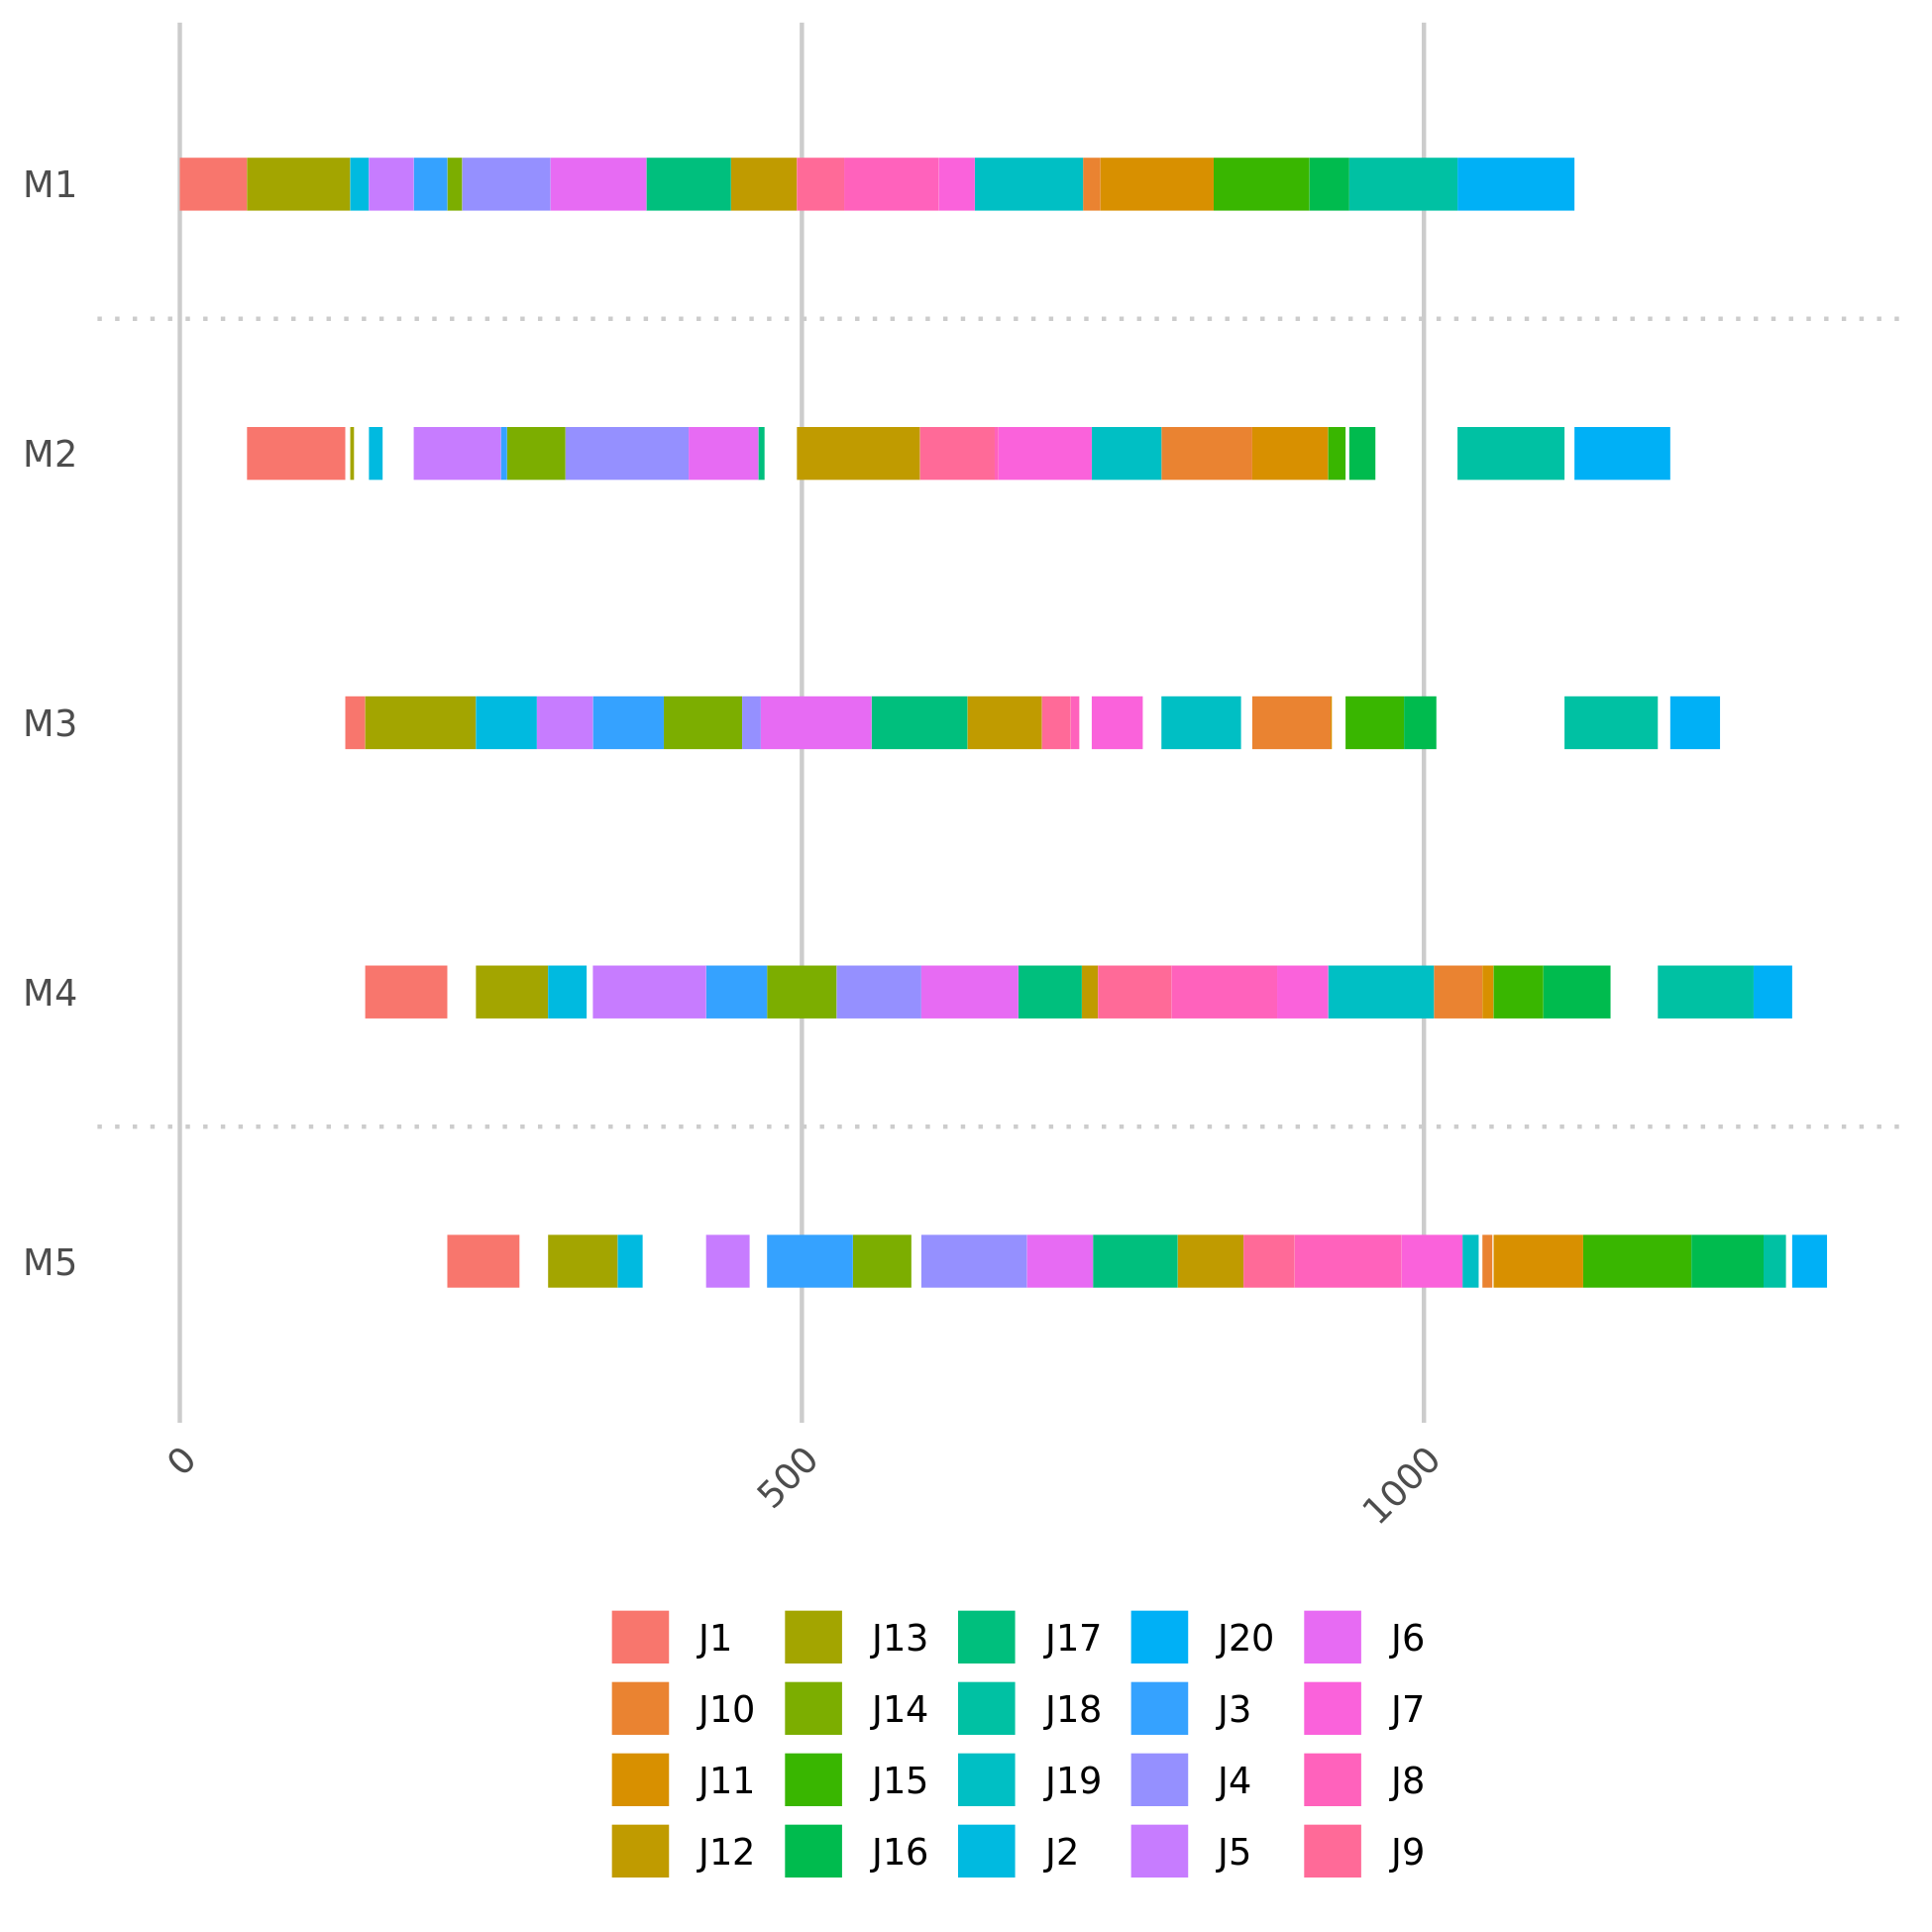
\includegraphics[width=\linewidth]{5_20_GC_1.png}
				\captionof{figure}{Gantt Chart for file 1.txt}
				
				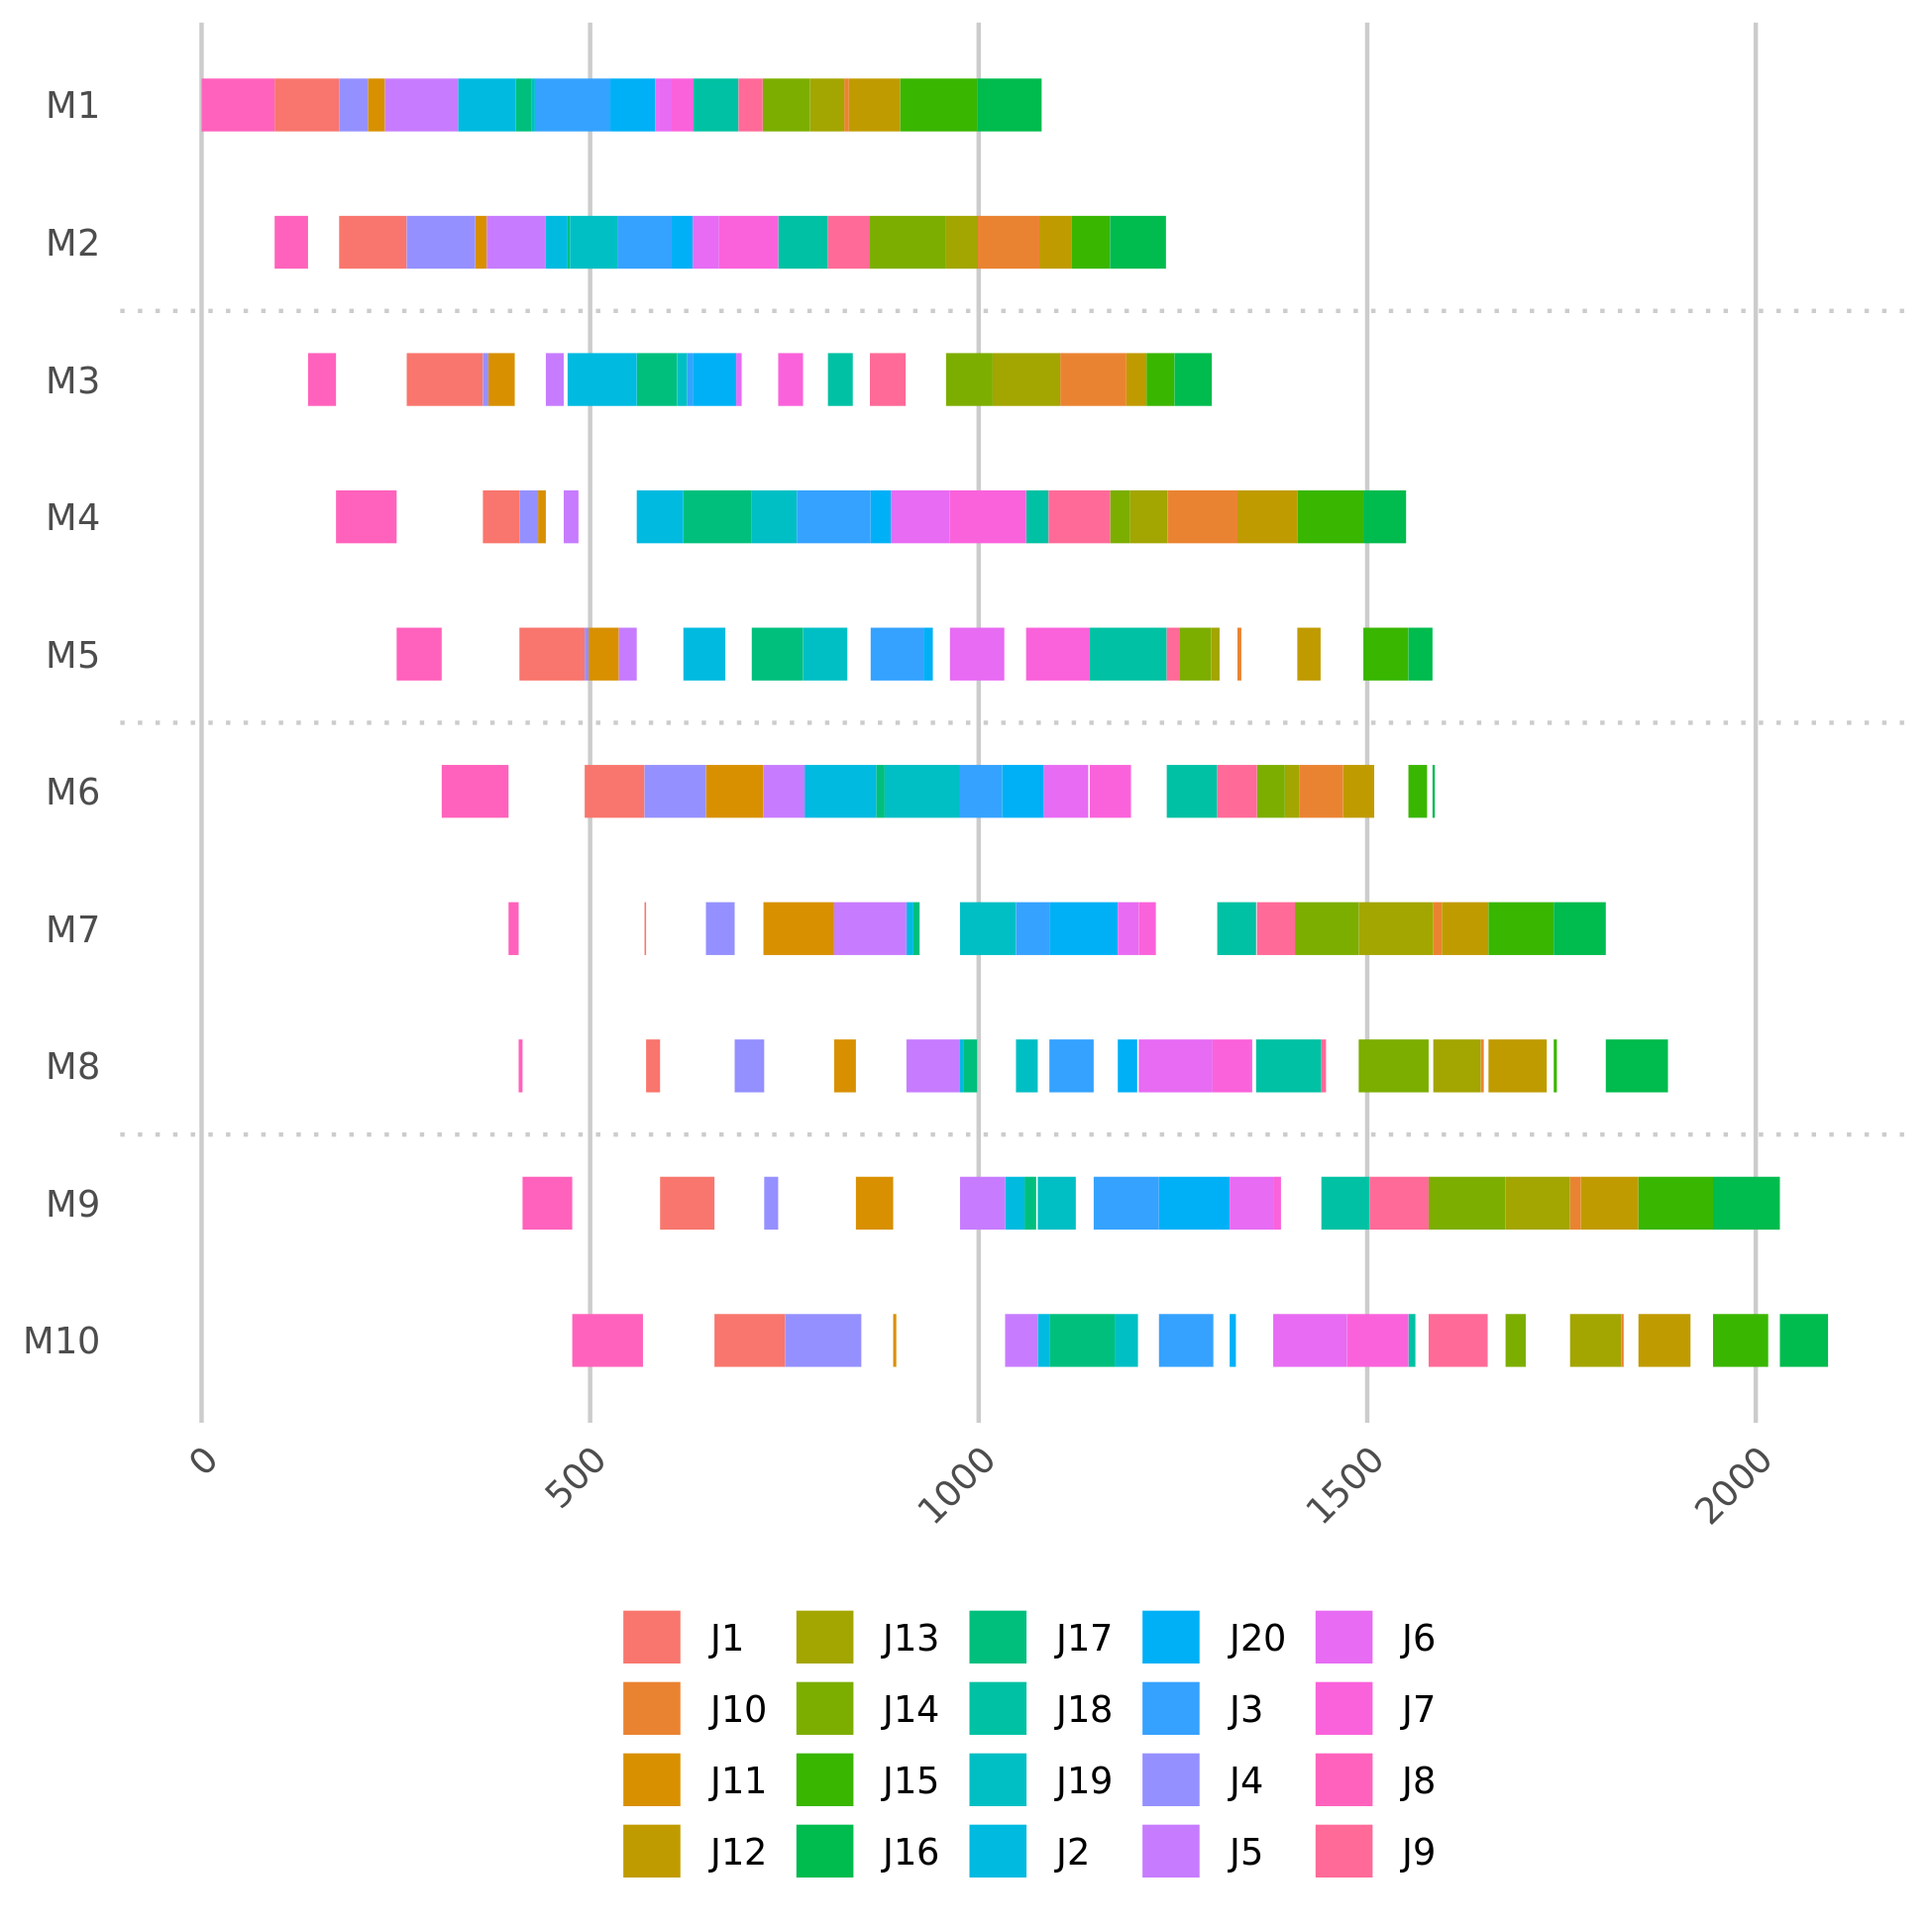
\includegraphics[width=\linewidth]{10_20_GC_1.png}
				\captionof{figure}{Gantt Chart for file 11.txt}
				
				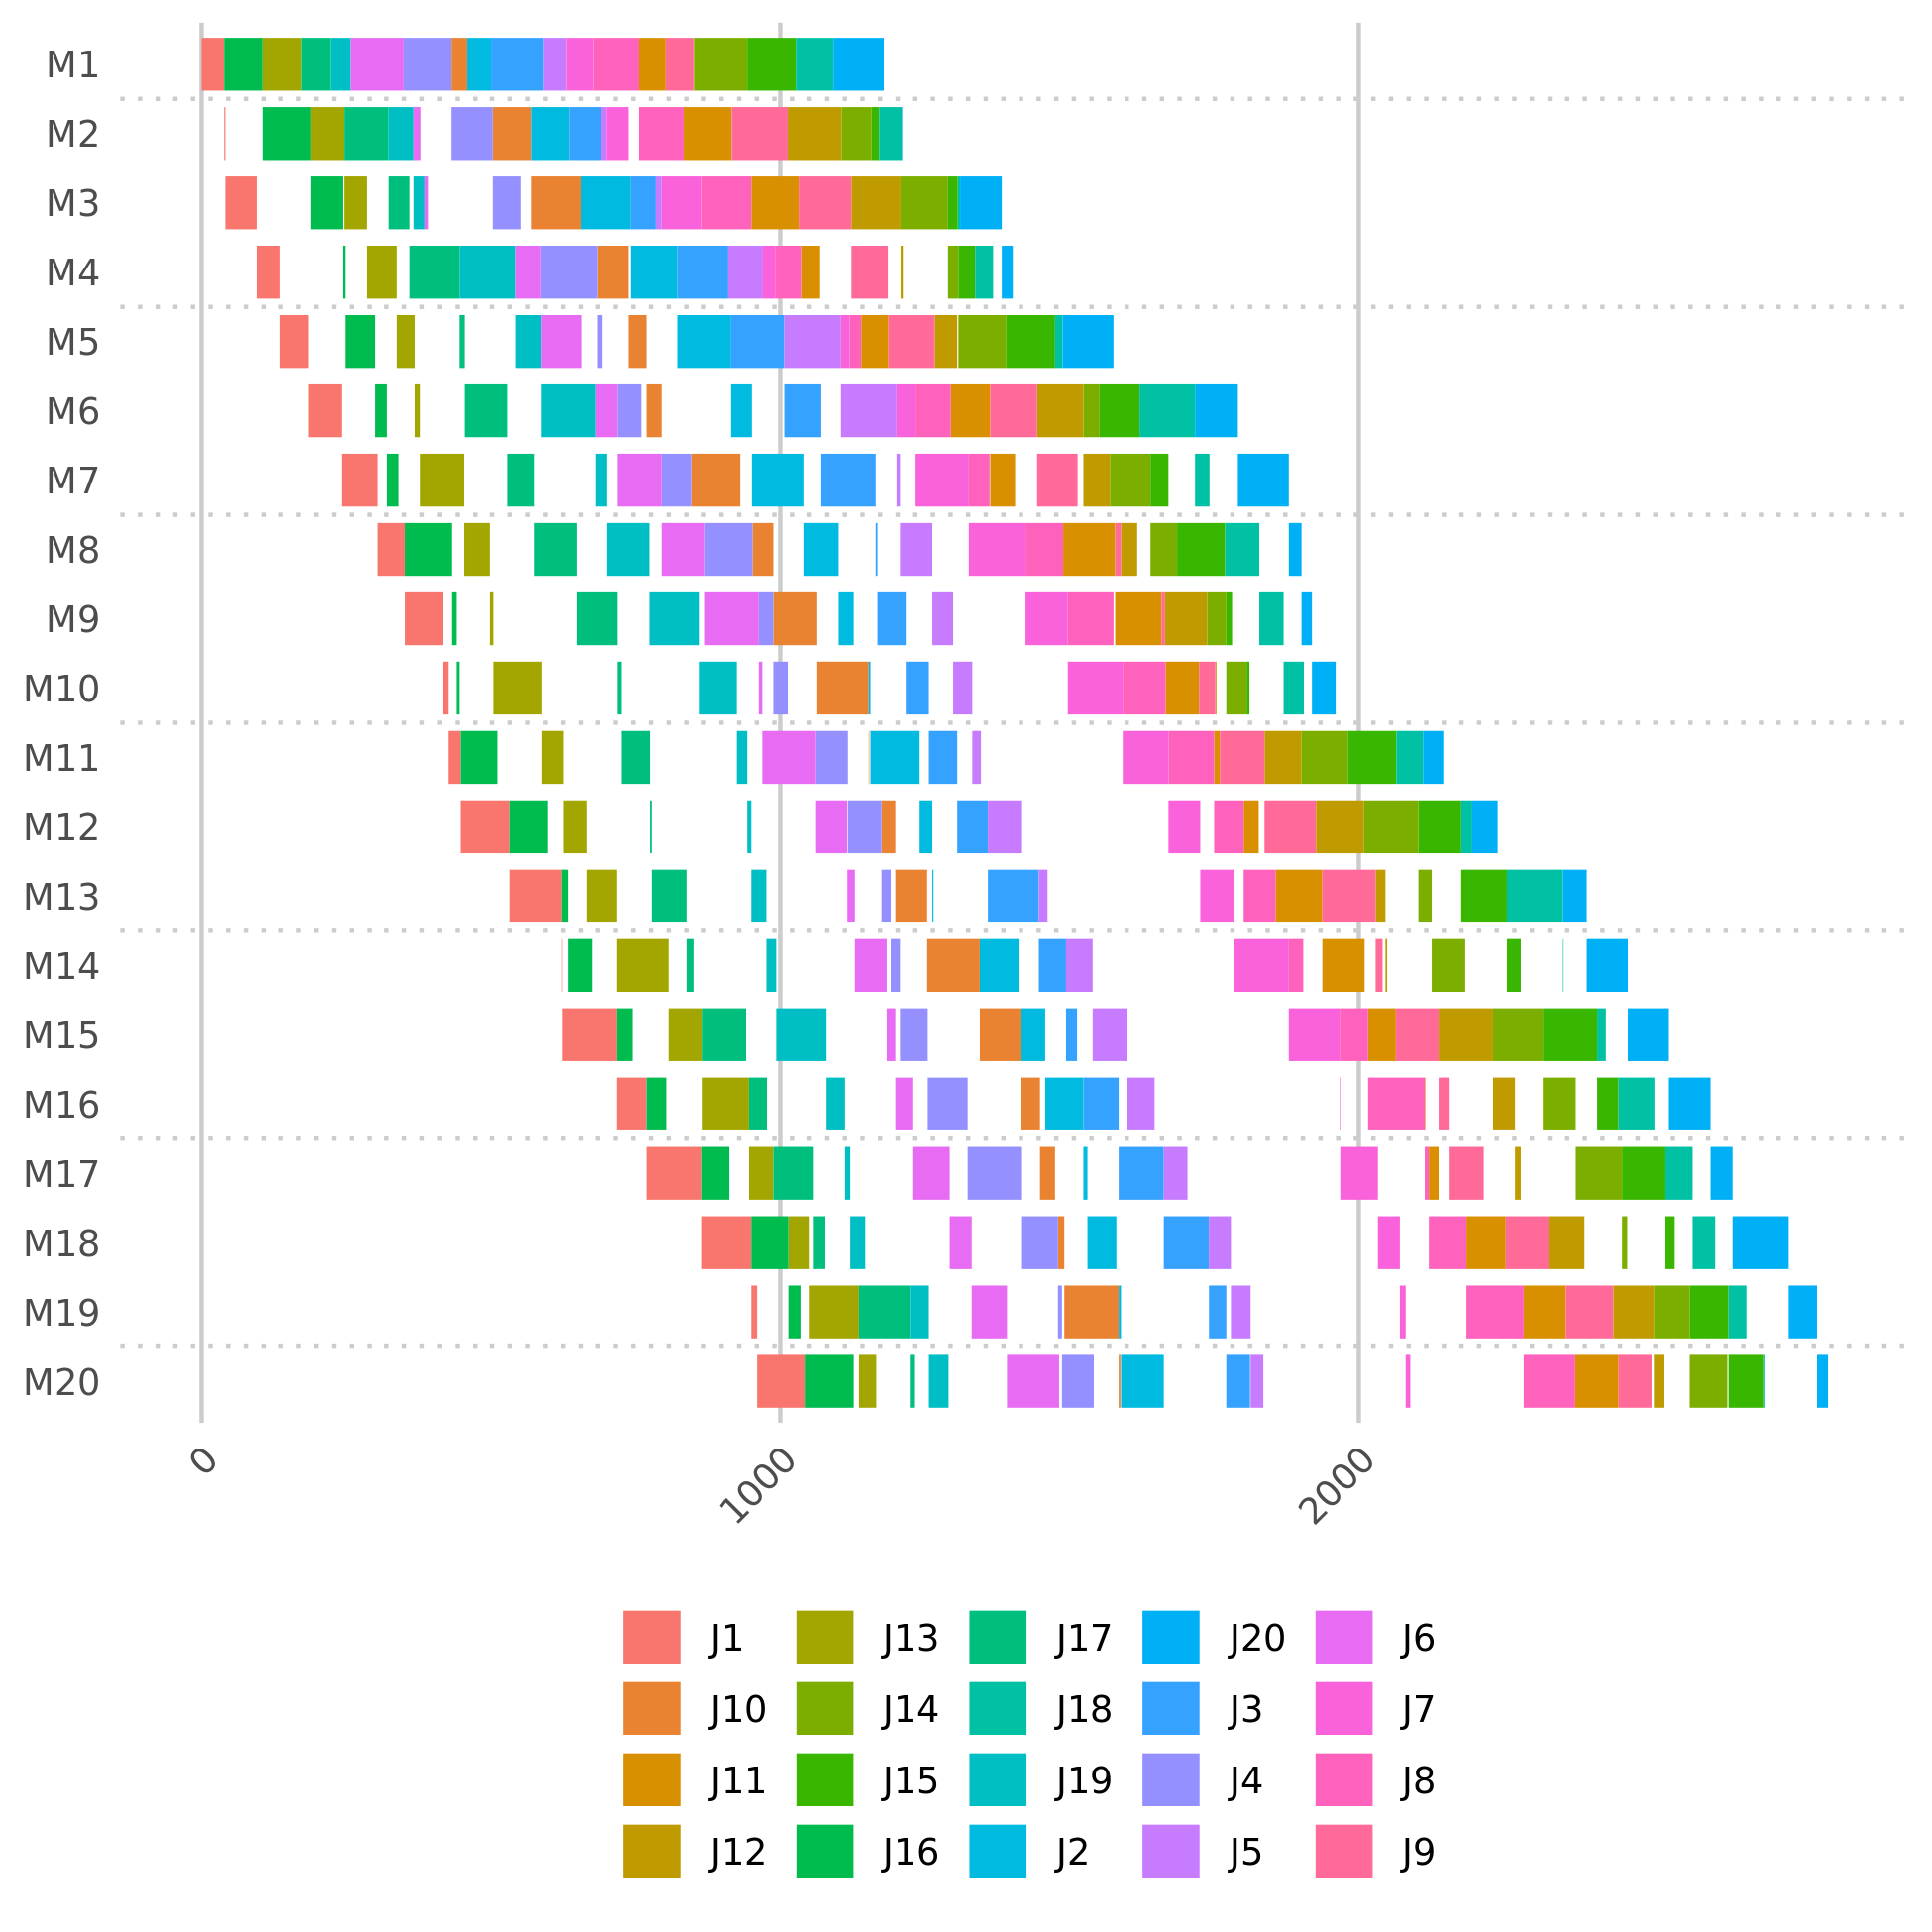
\includegraphics[width=\linewidth]{20_20_GC_1.png}
				\captionof{figure}{Gantt Chart for file 21.txt}
				
				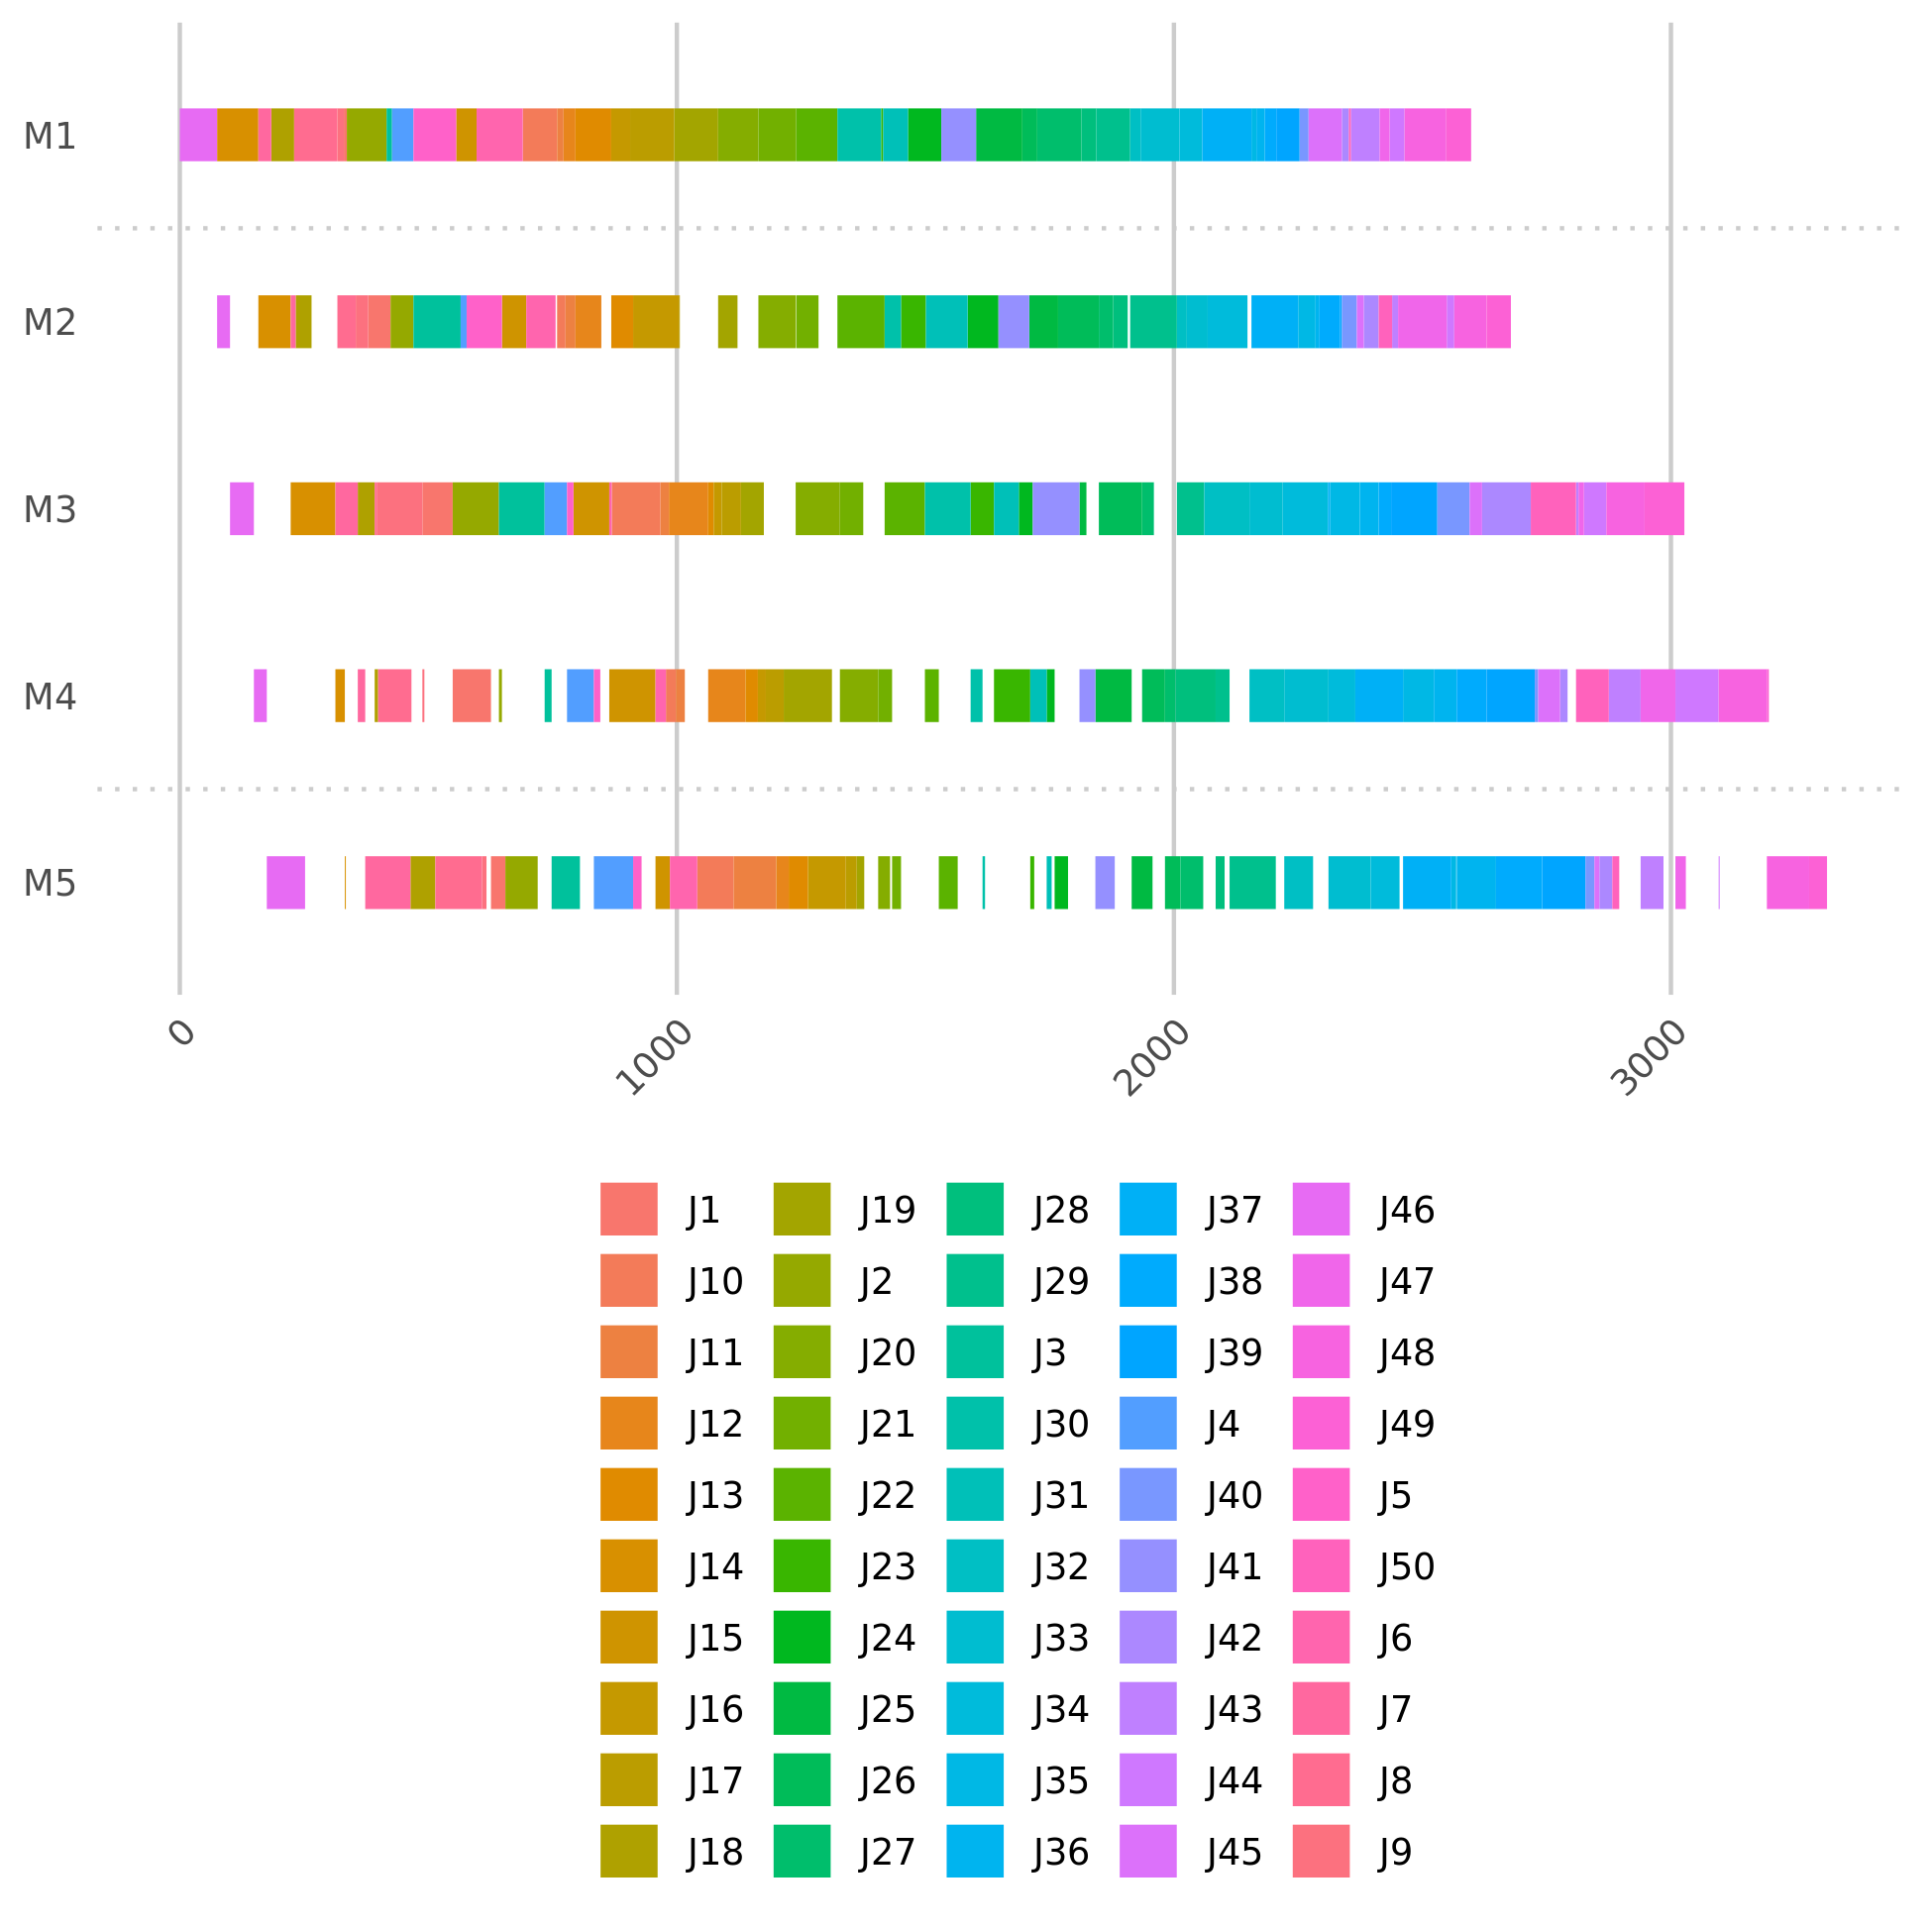
\includegraphics[width=\linewidth]{5_50_GC_1.png}
				\captionof{figure}{Gantt Chart for file 31.txt}
				
				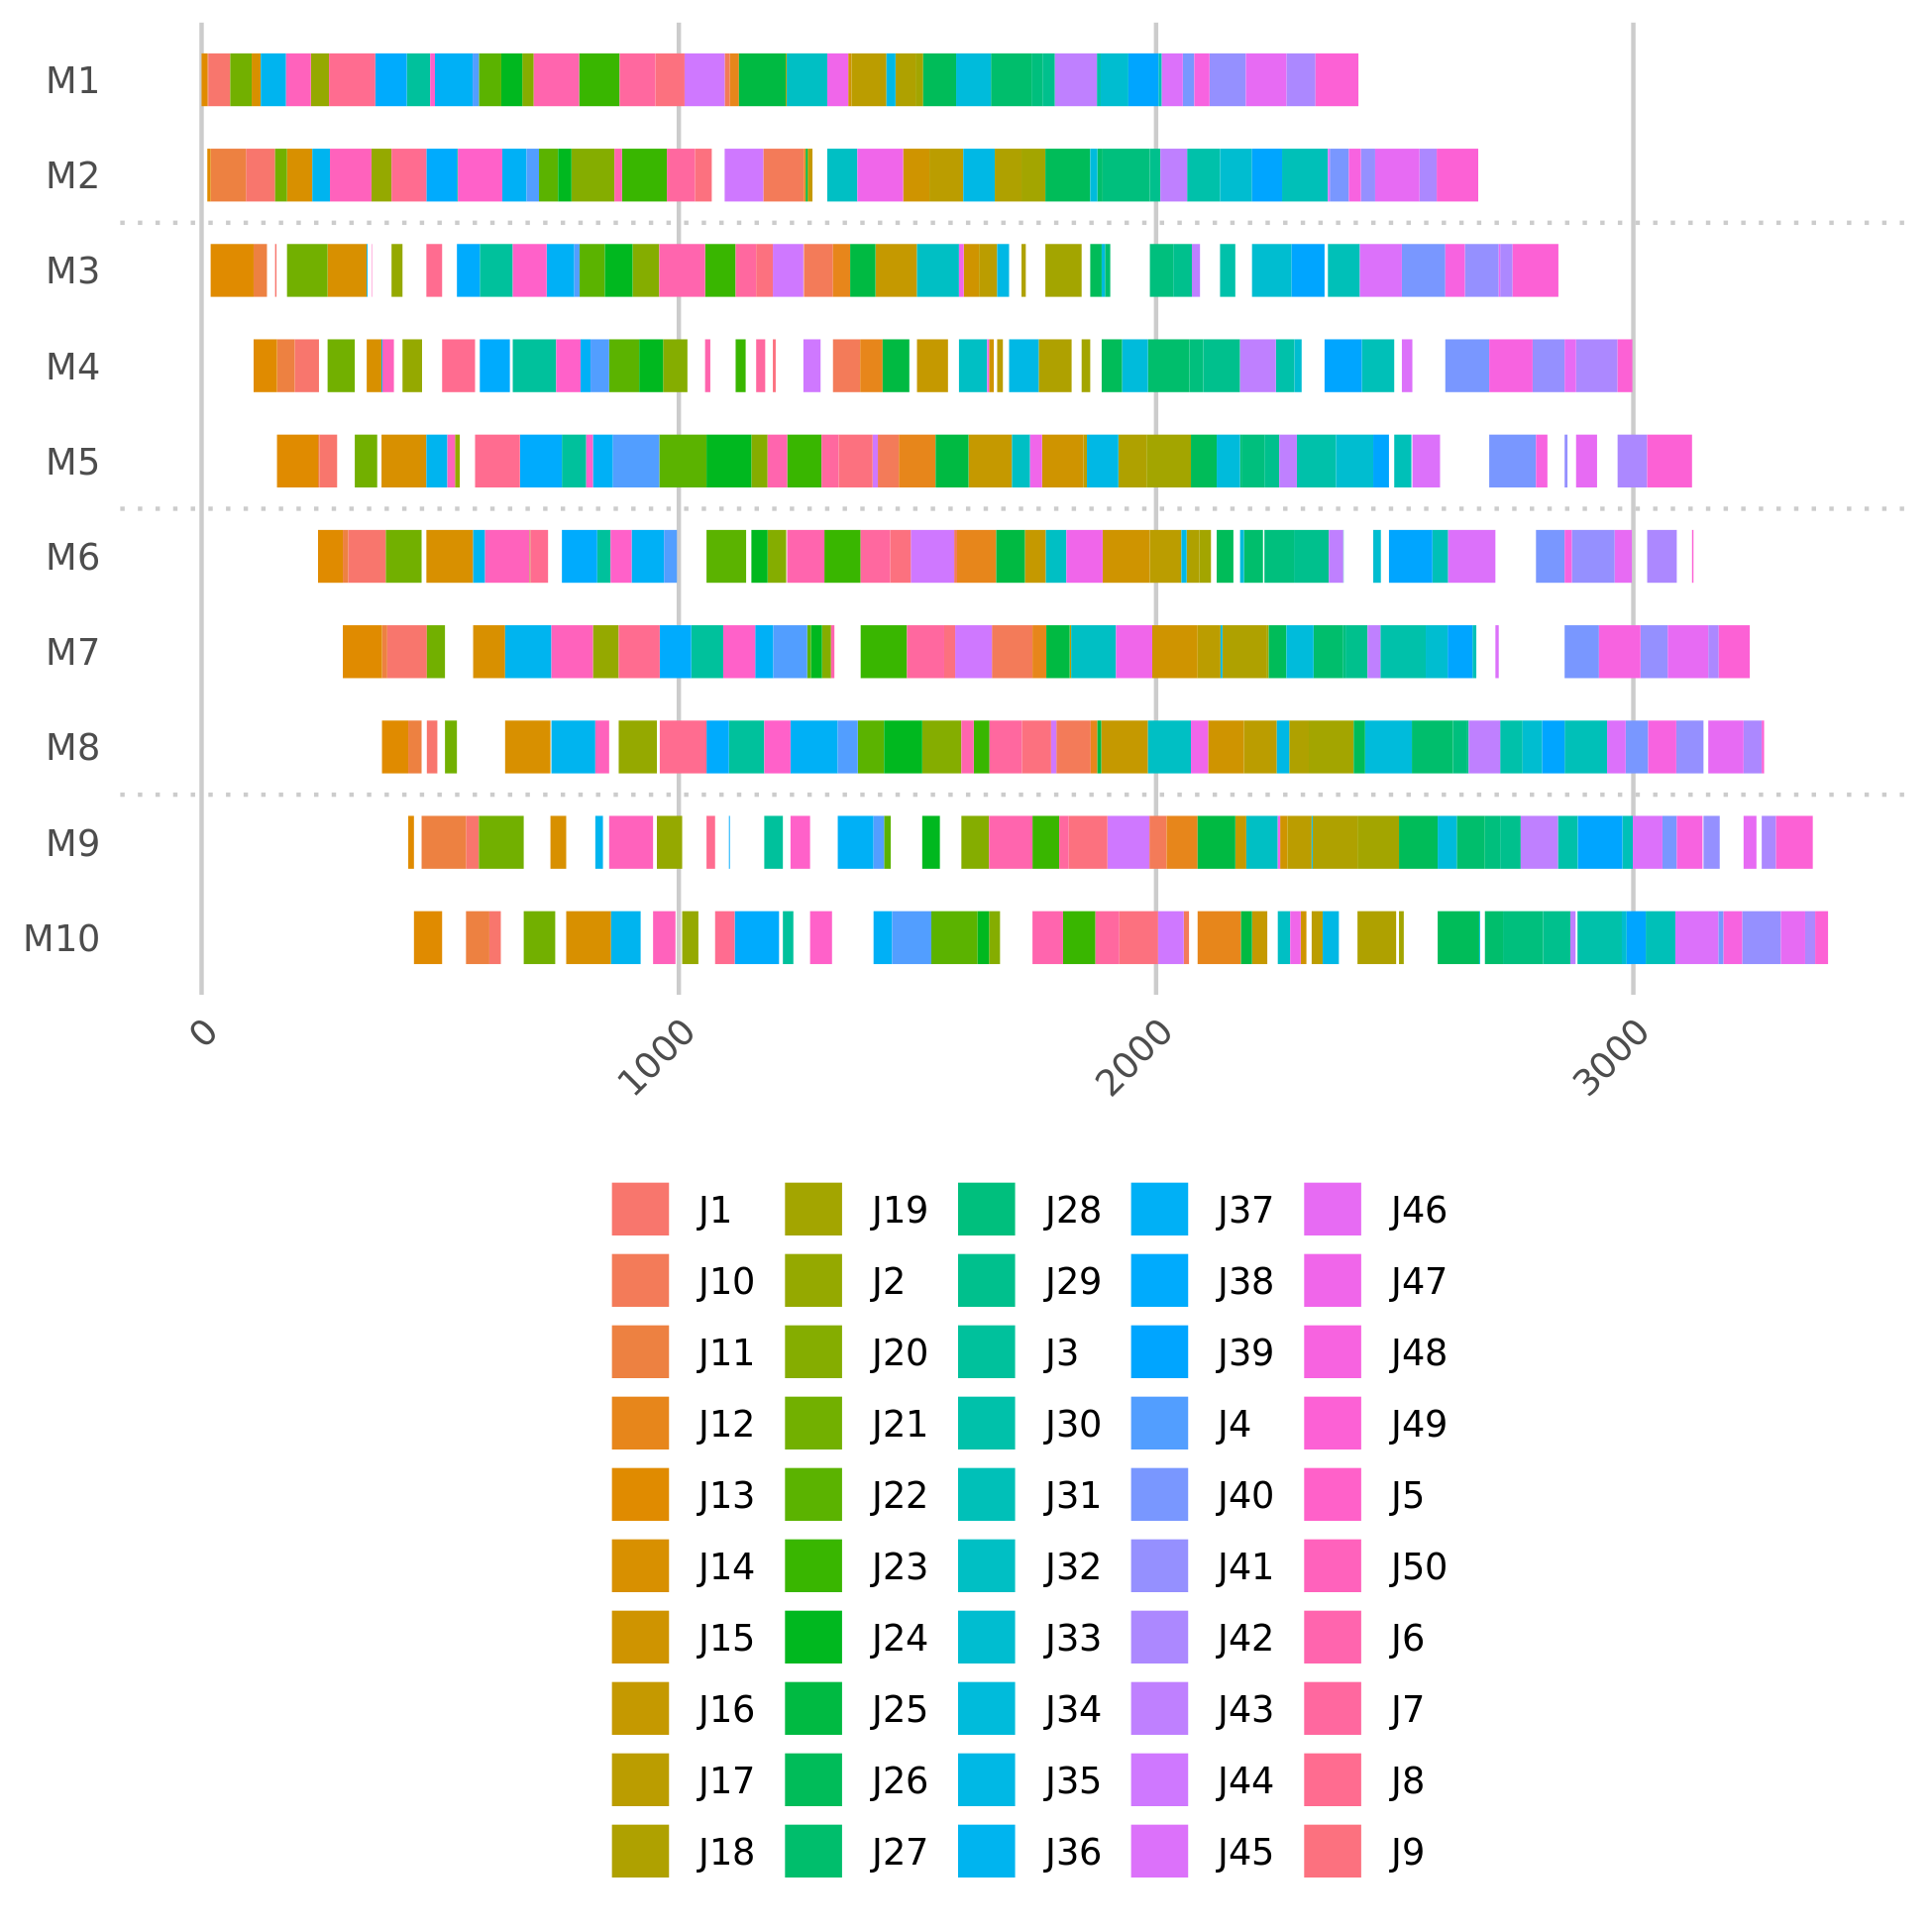
\includegraphics[width=\linewidth]{10_50_GC_1.png}
				\captionof{figure}{Gantt Chart for file 41.txt}
				
				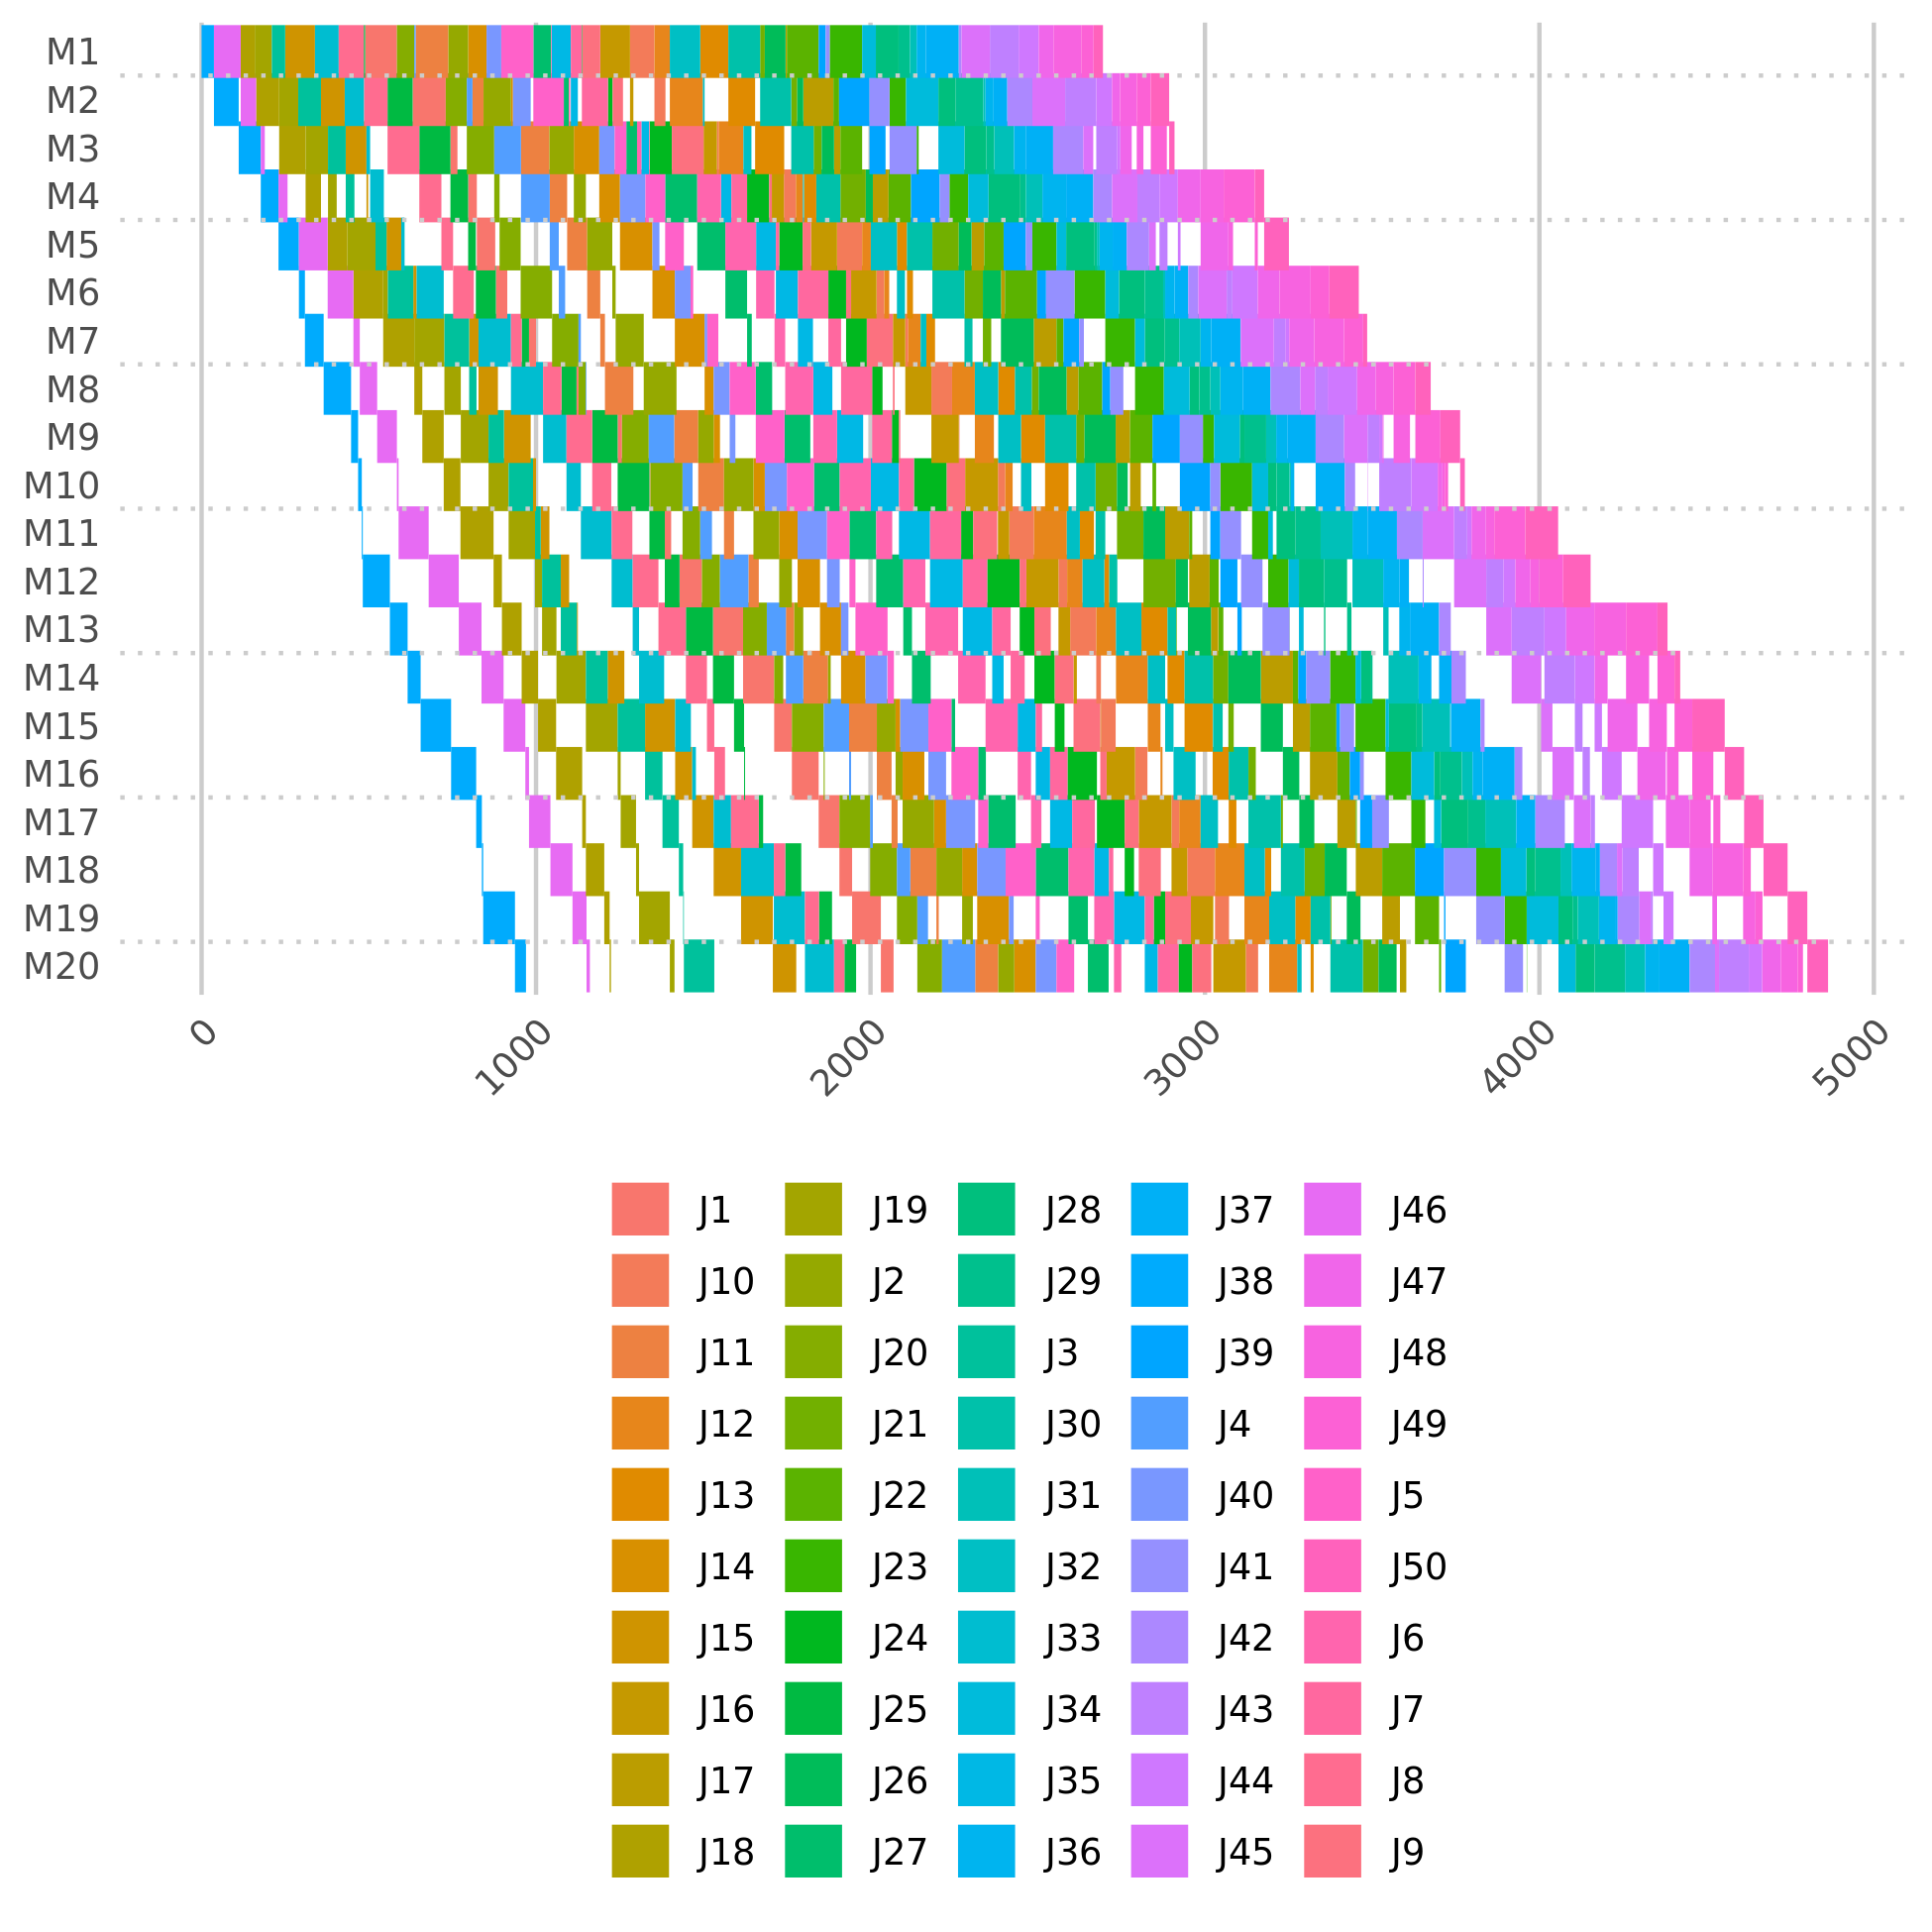
\includegraphics[width=\linewidth]{20_50_GC_1.png}
				\captionof{figure}{Gantt Chart for file 51.txt}
				
				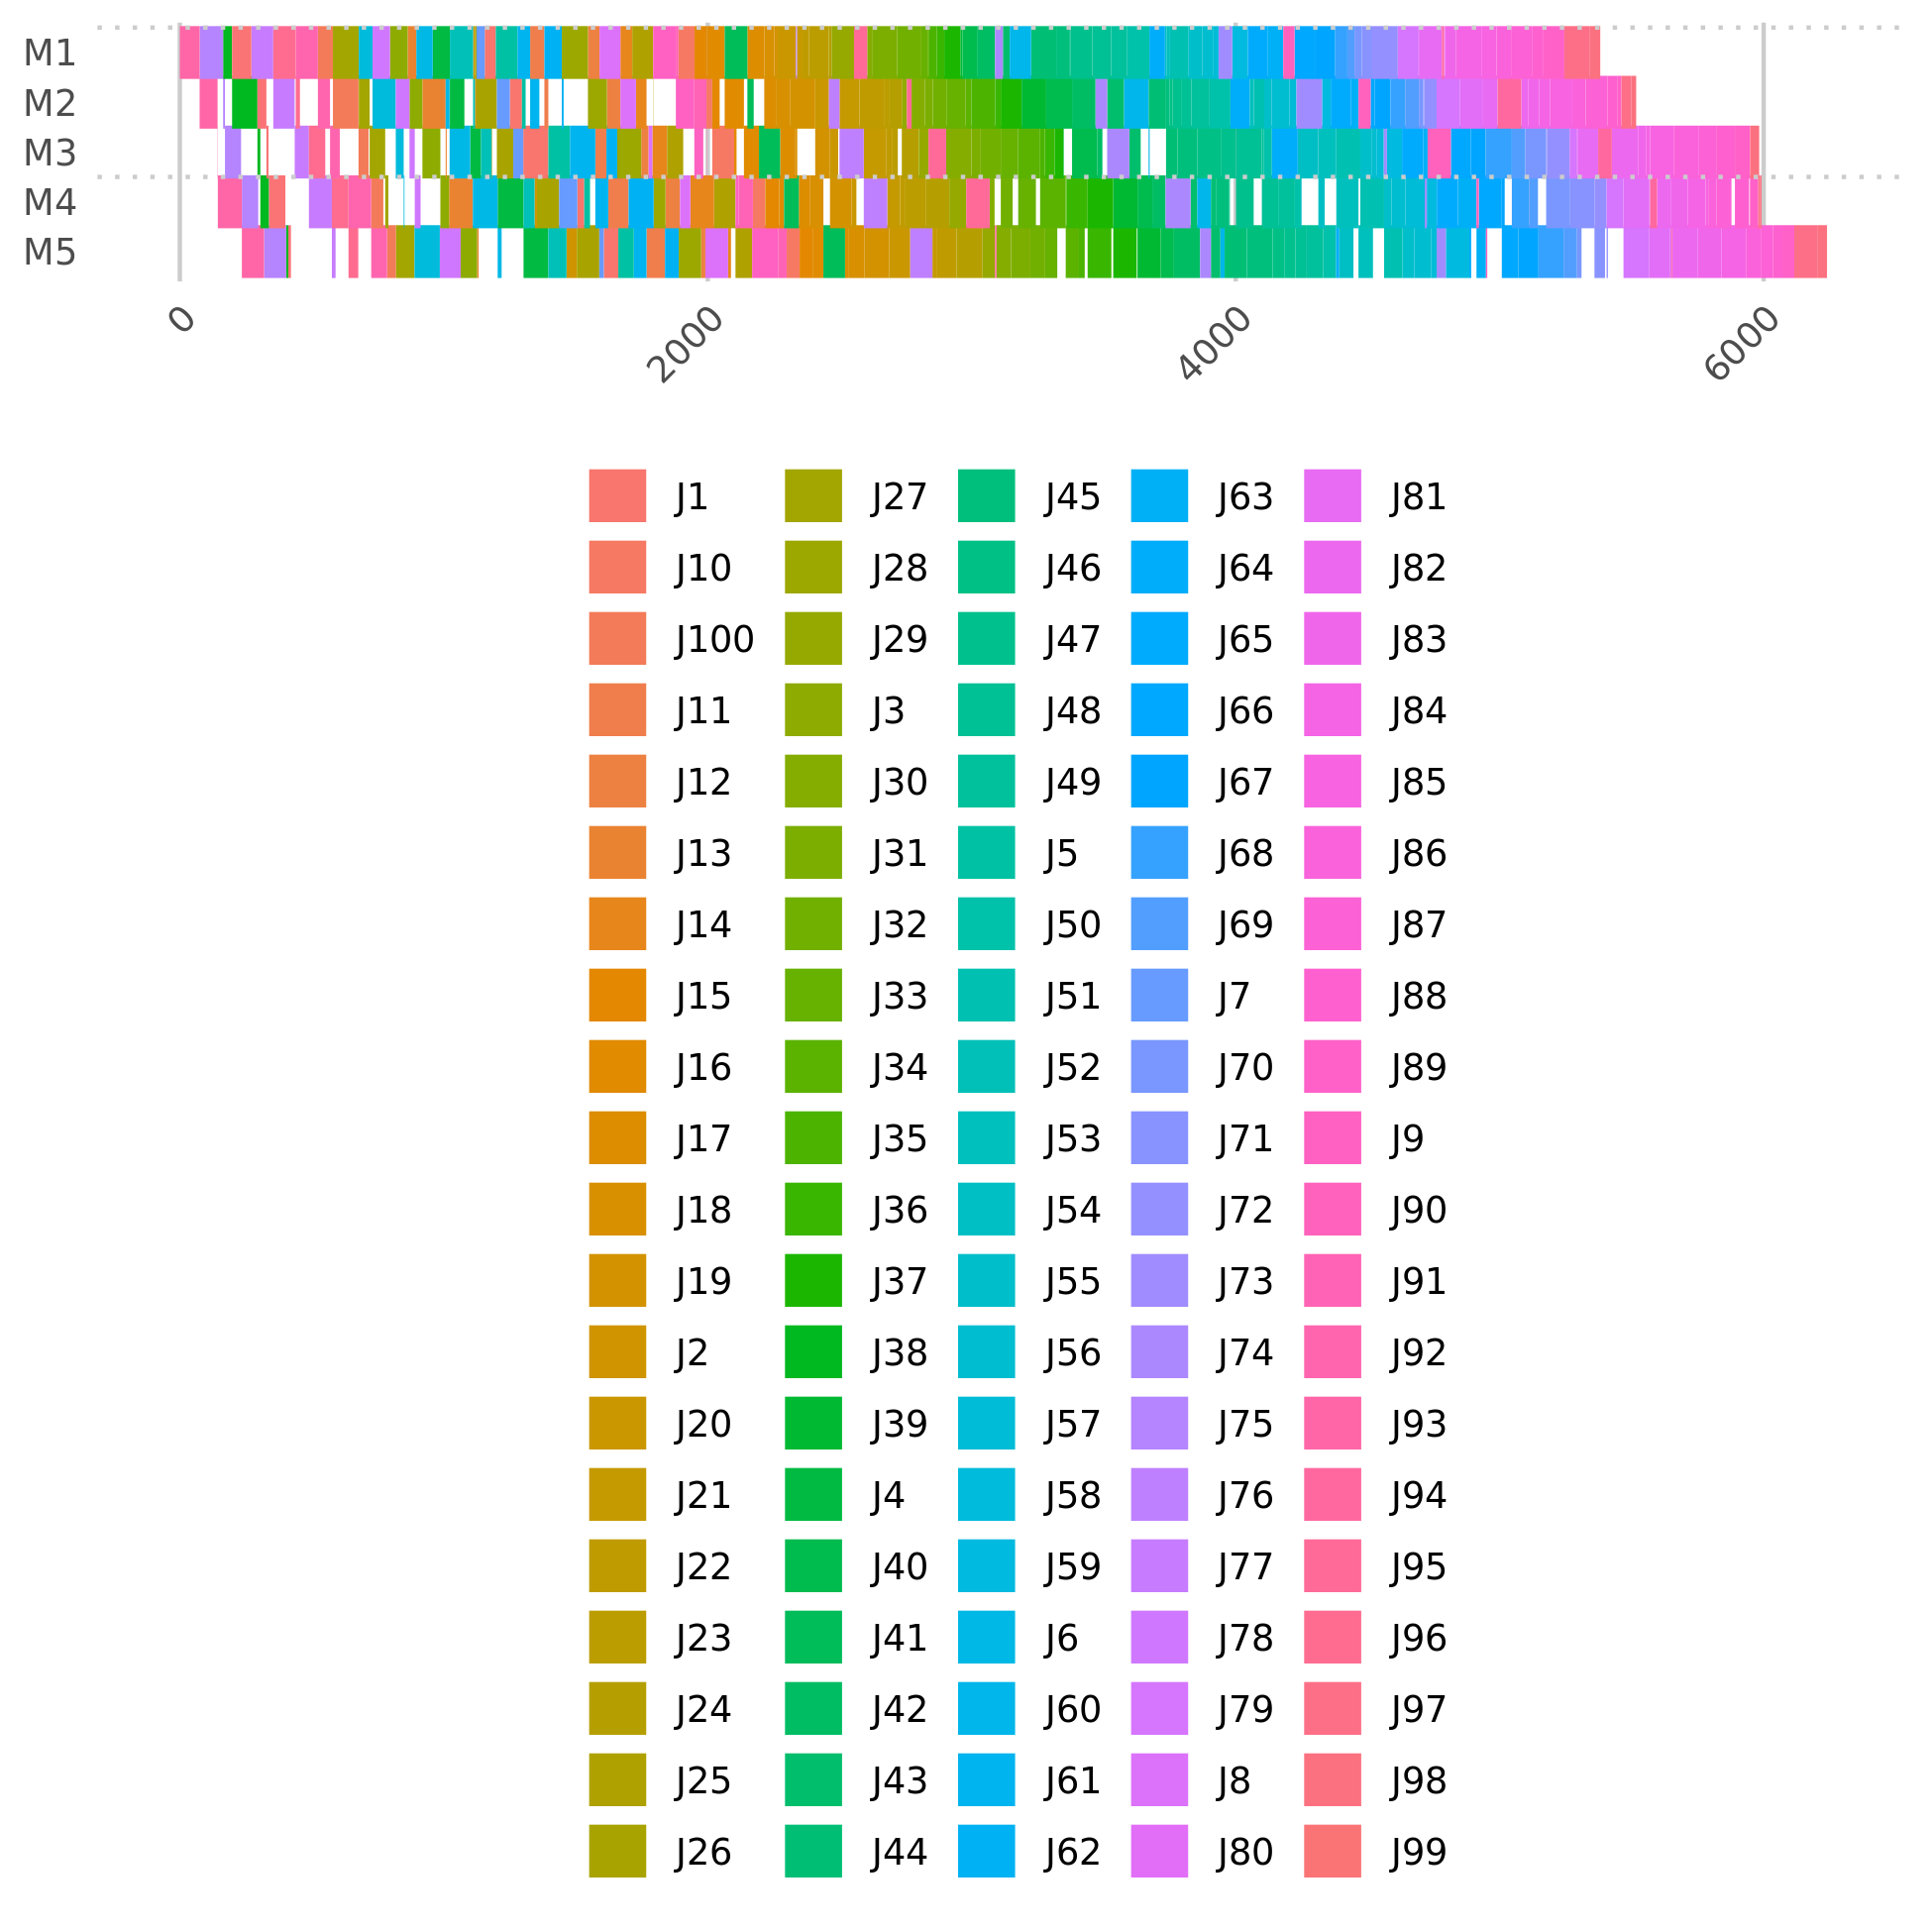
\includegraphics[width=\linewidth]{5_100_GC_1.png}
				\captionof{figure}{Gantt Chart for file 61.txt}
				
				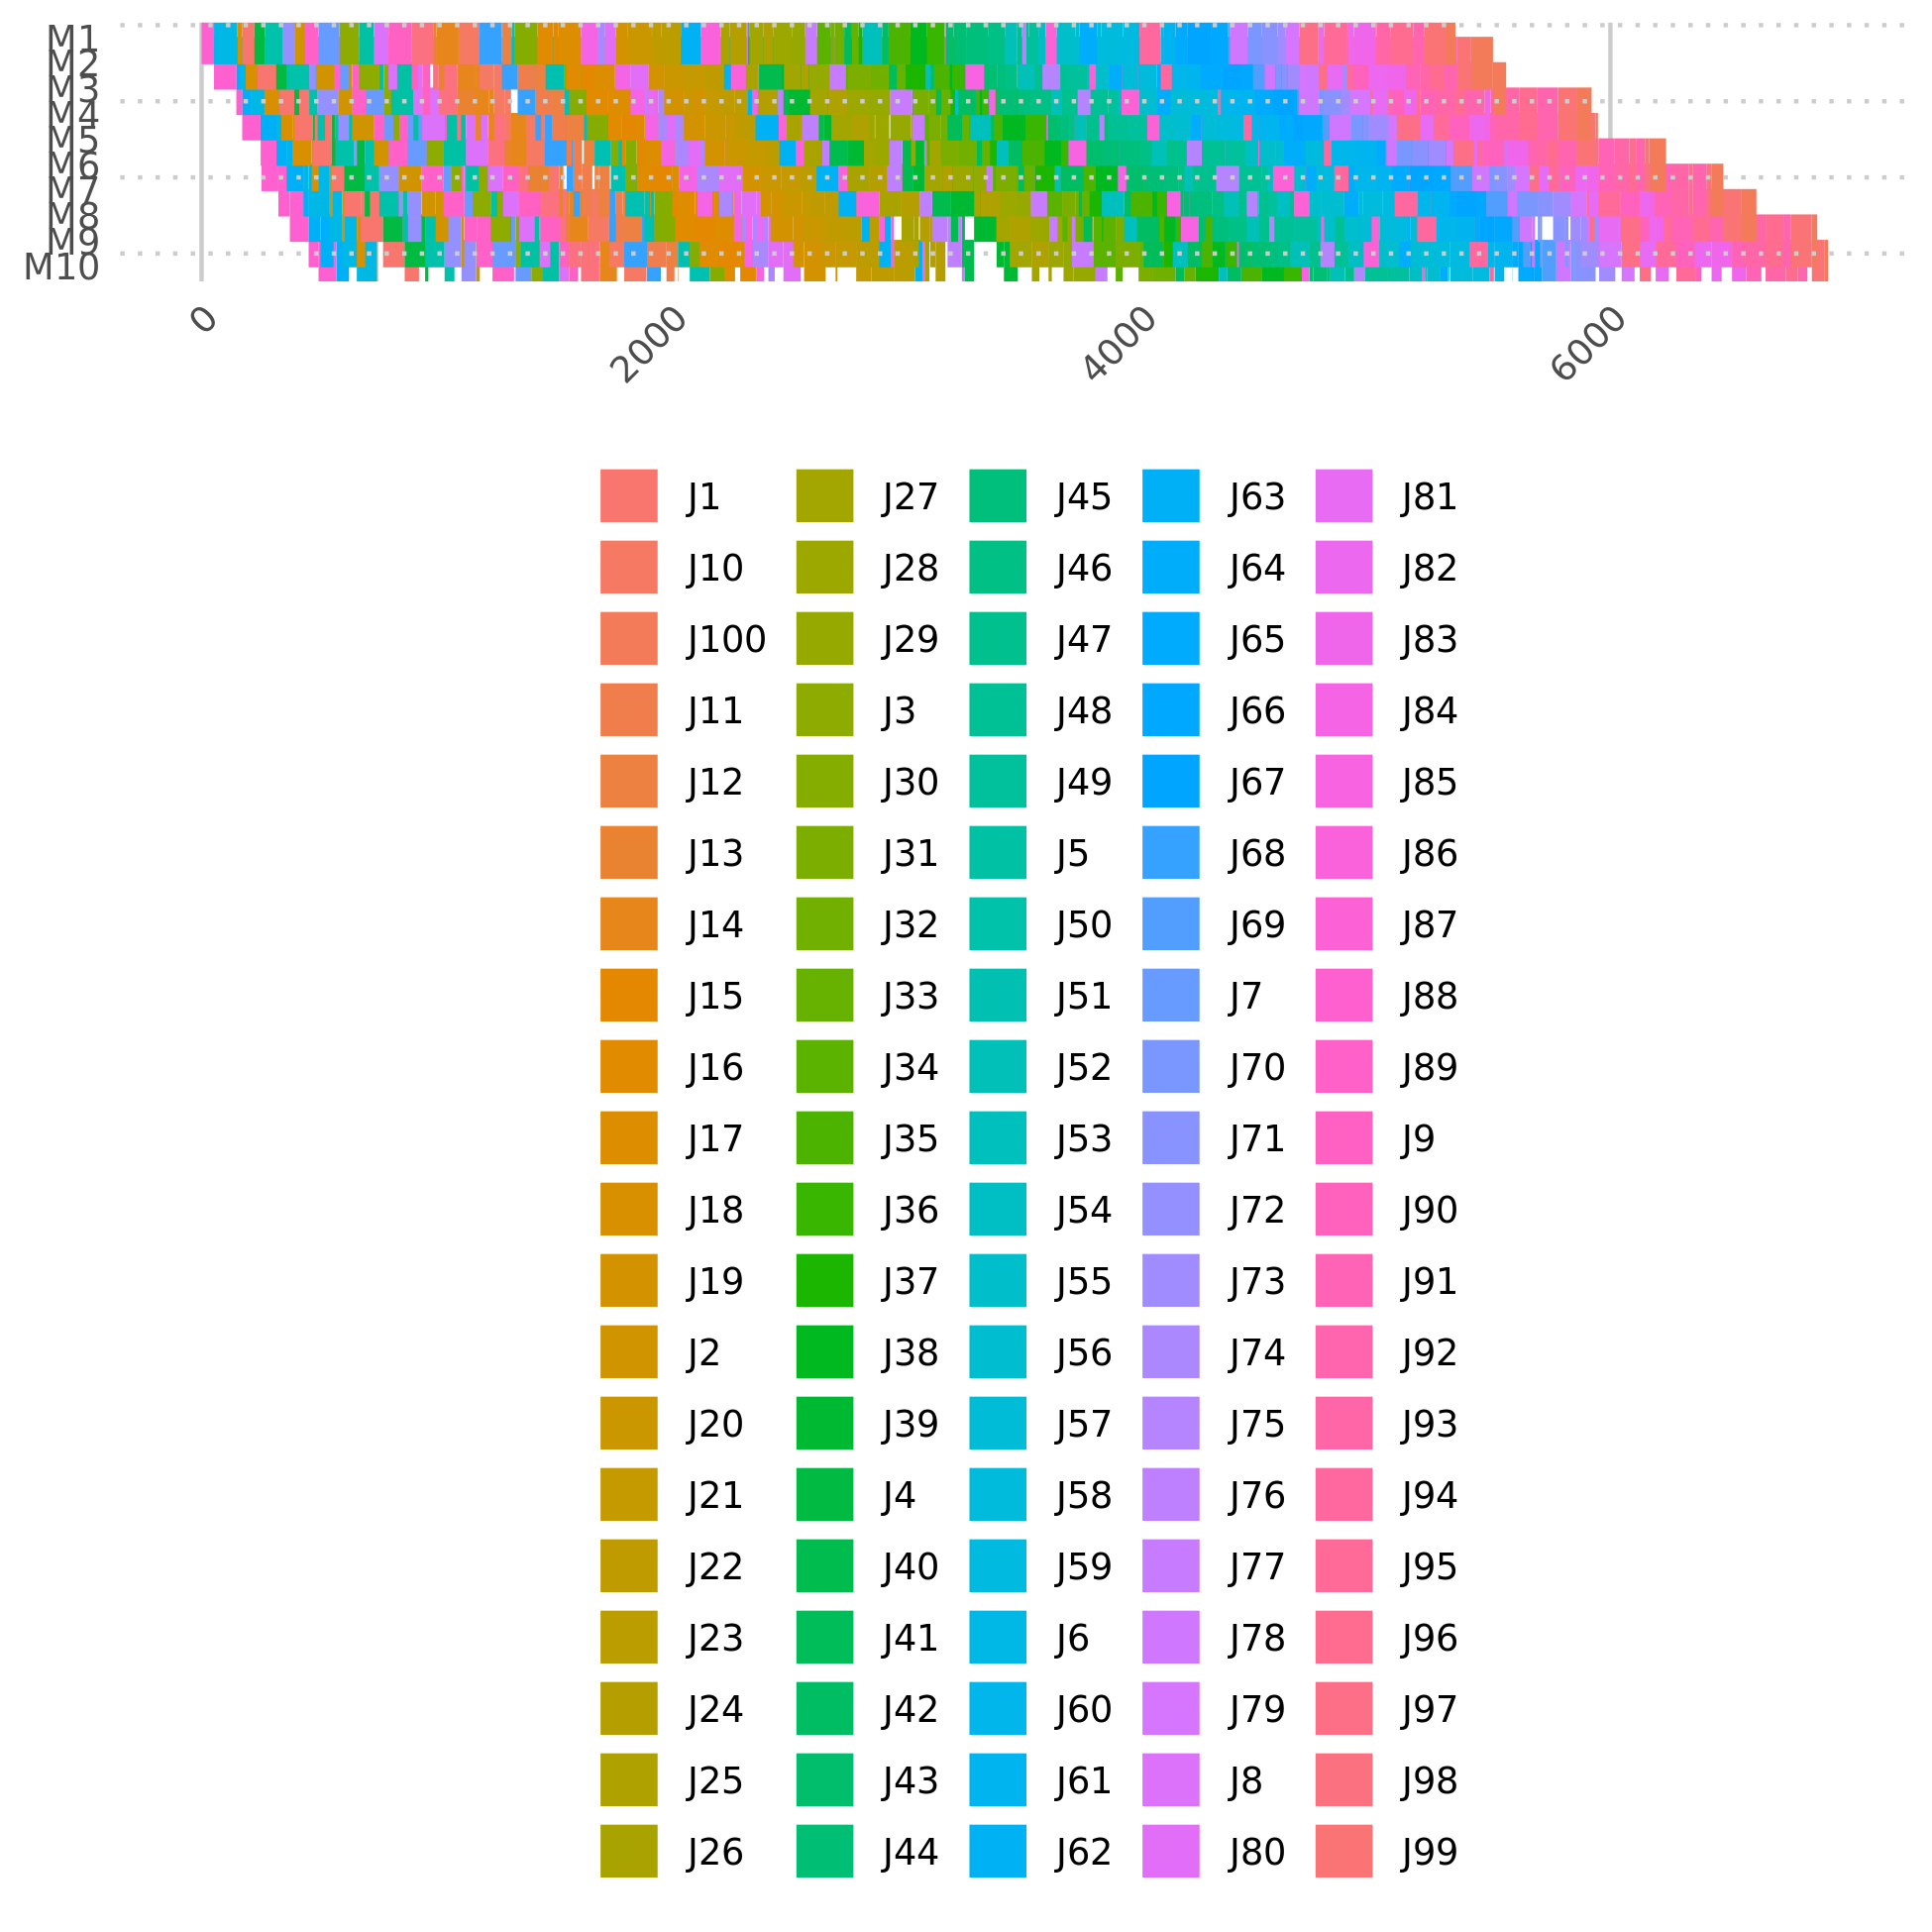
\includegraphics[width=\linewidth]{10_100_GC_1.png}
				\captionof{figure}{Gantt Chart for file 71.txt}
				
				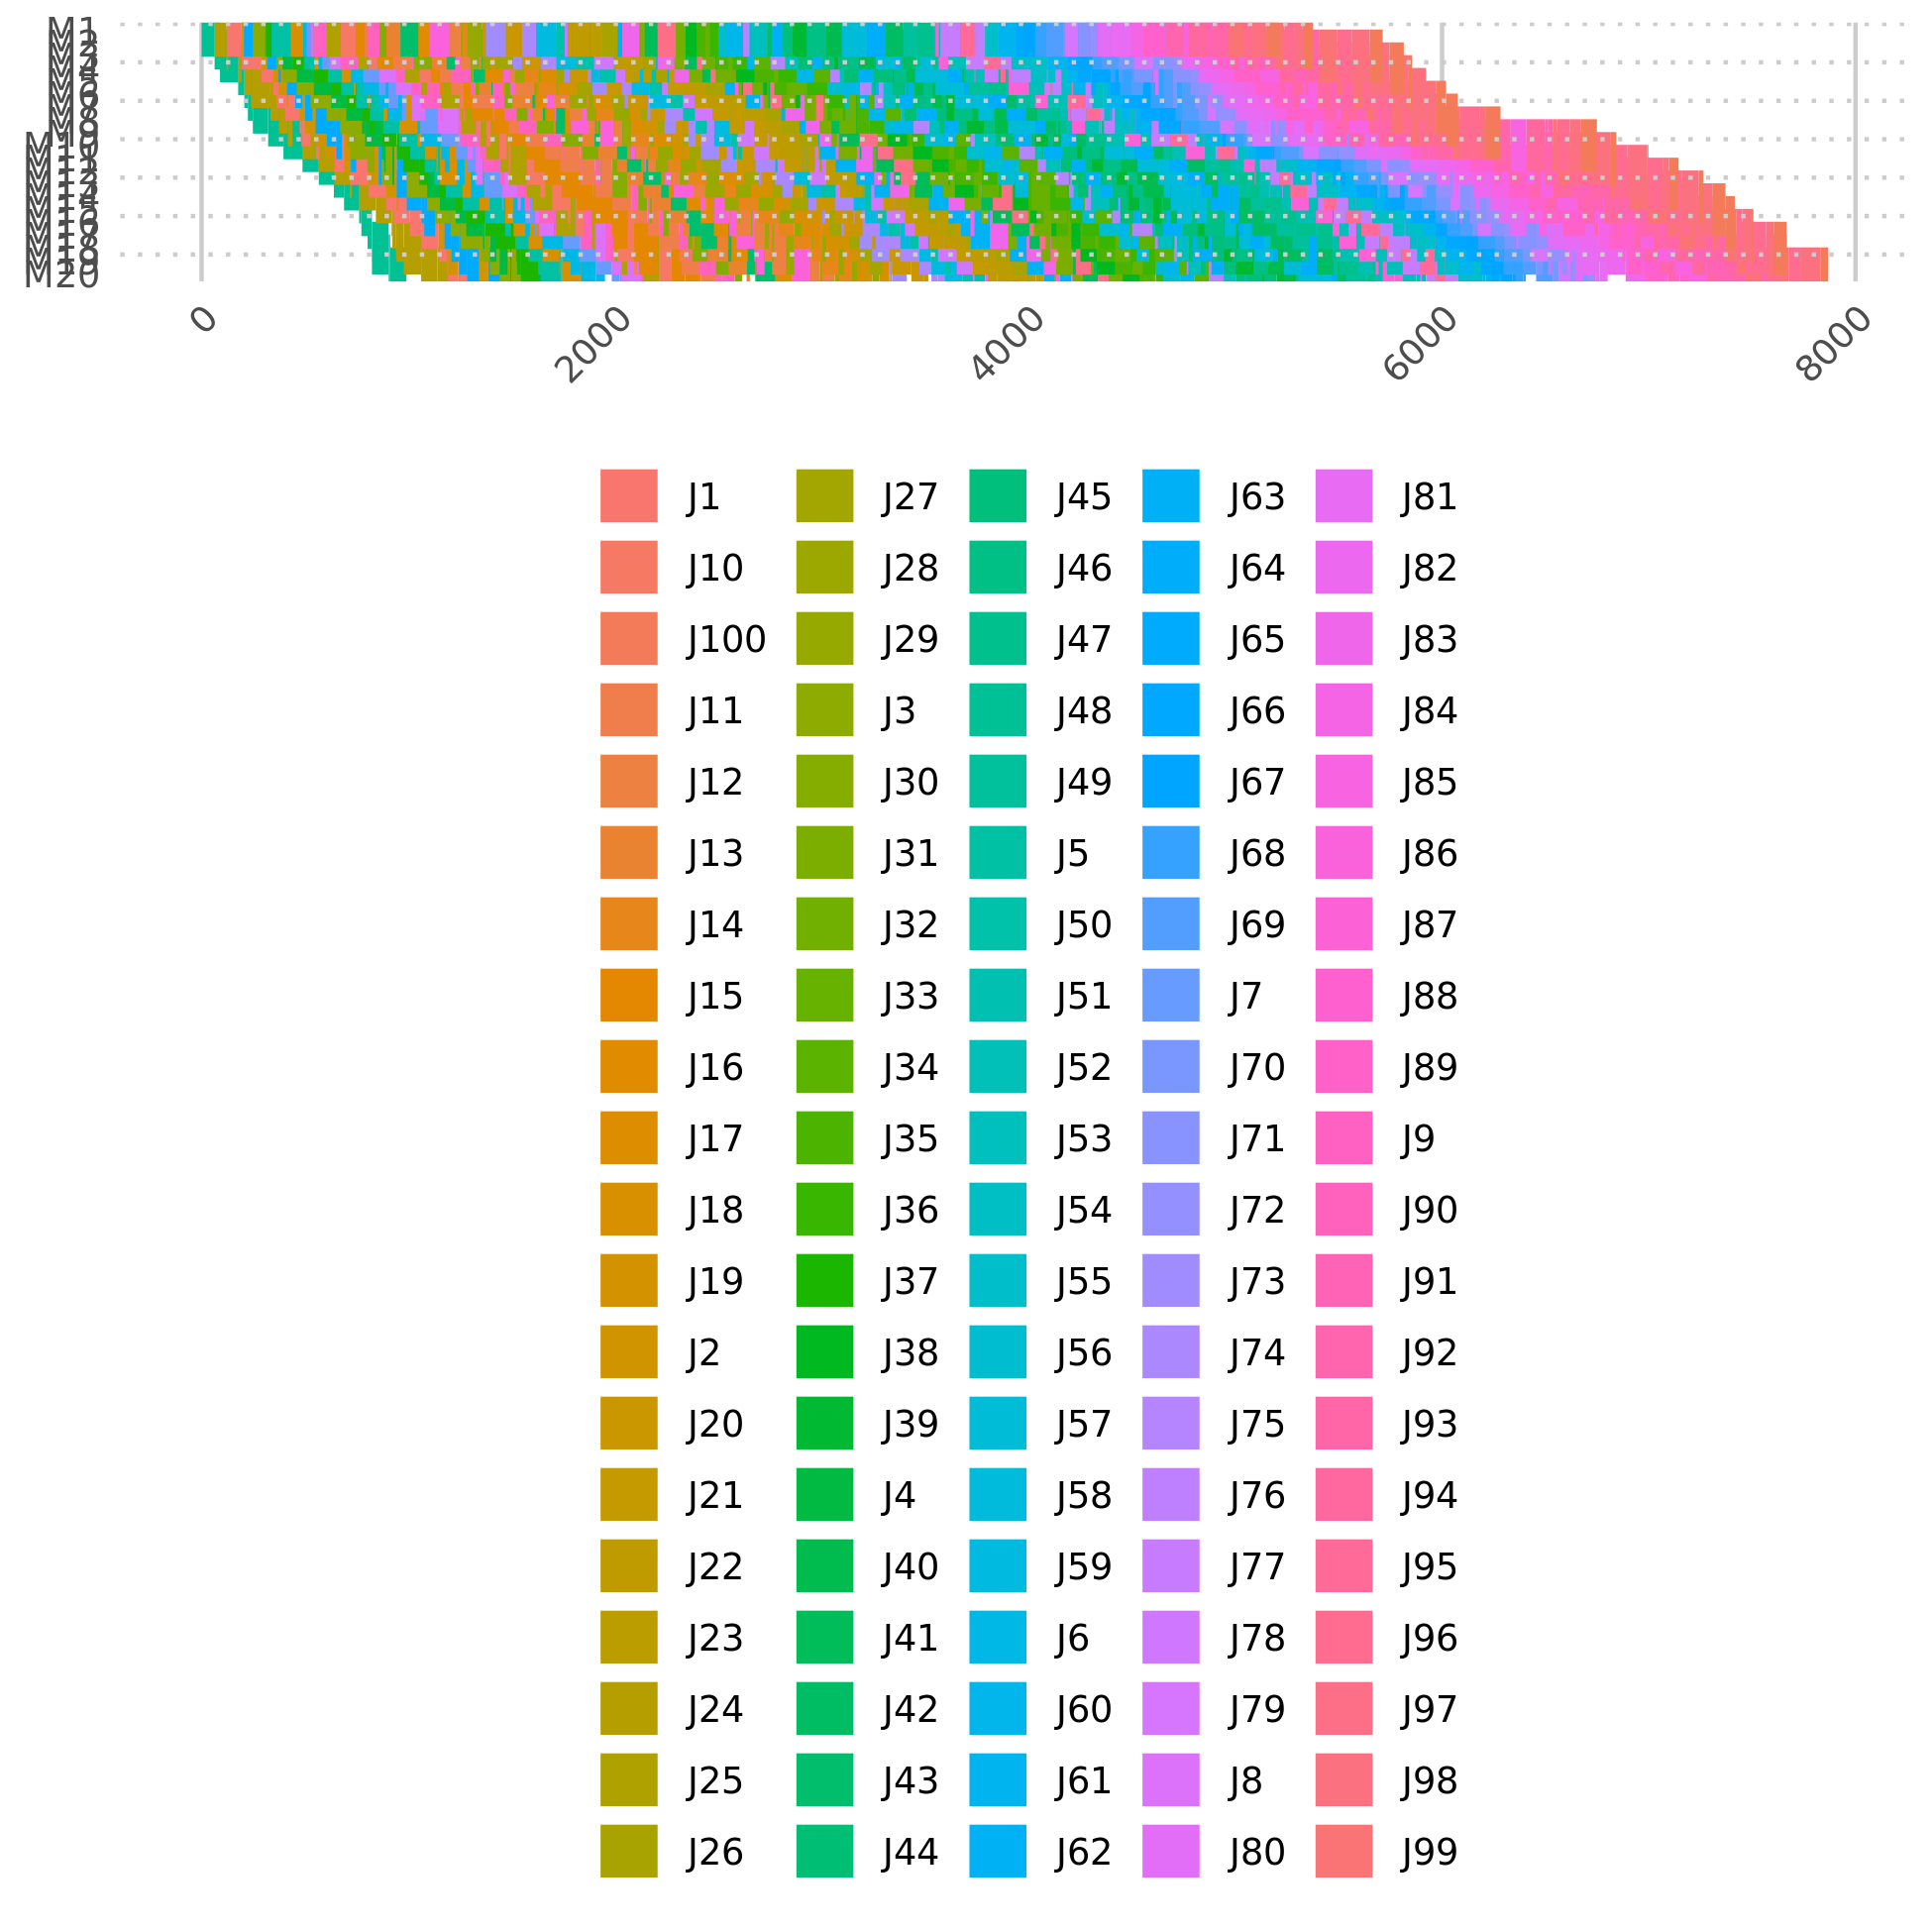
\includegraphics[width=\linewidth]{20_100_GC_1.png}
				\captionof{figure}{Gantt Chart for file 81.txt}
				
				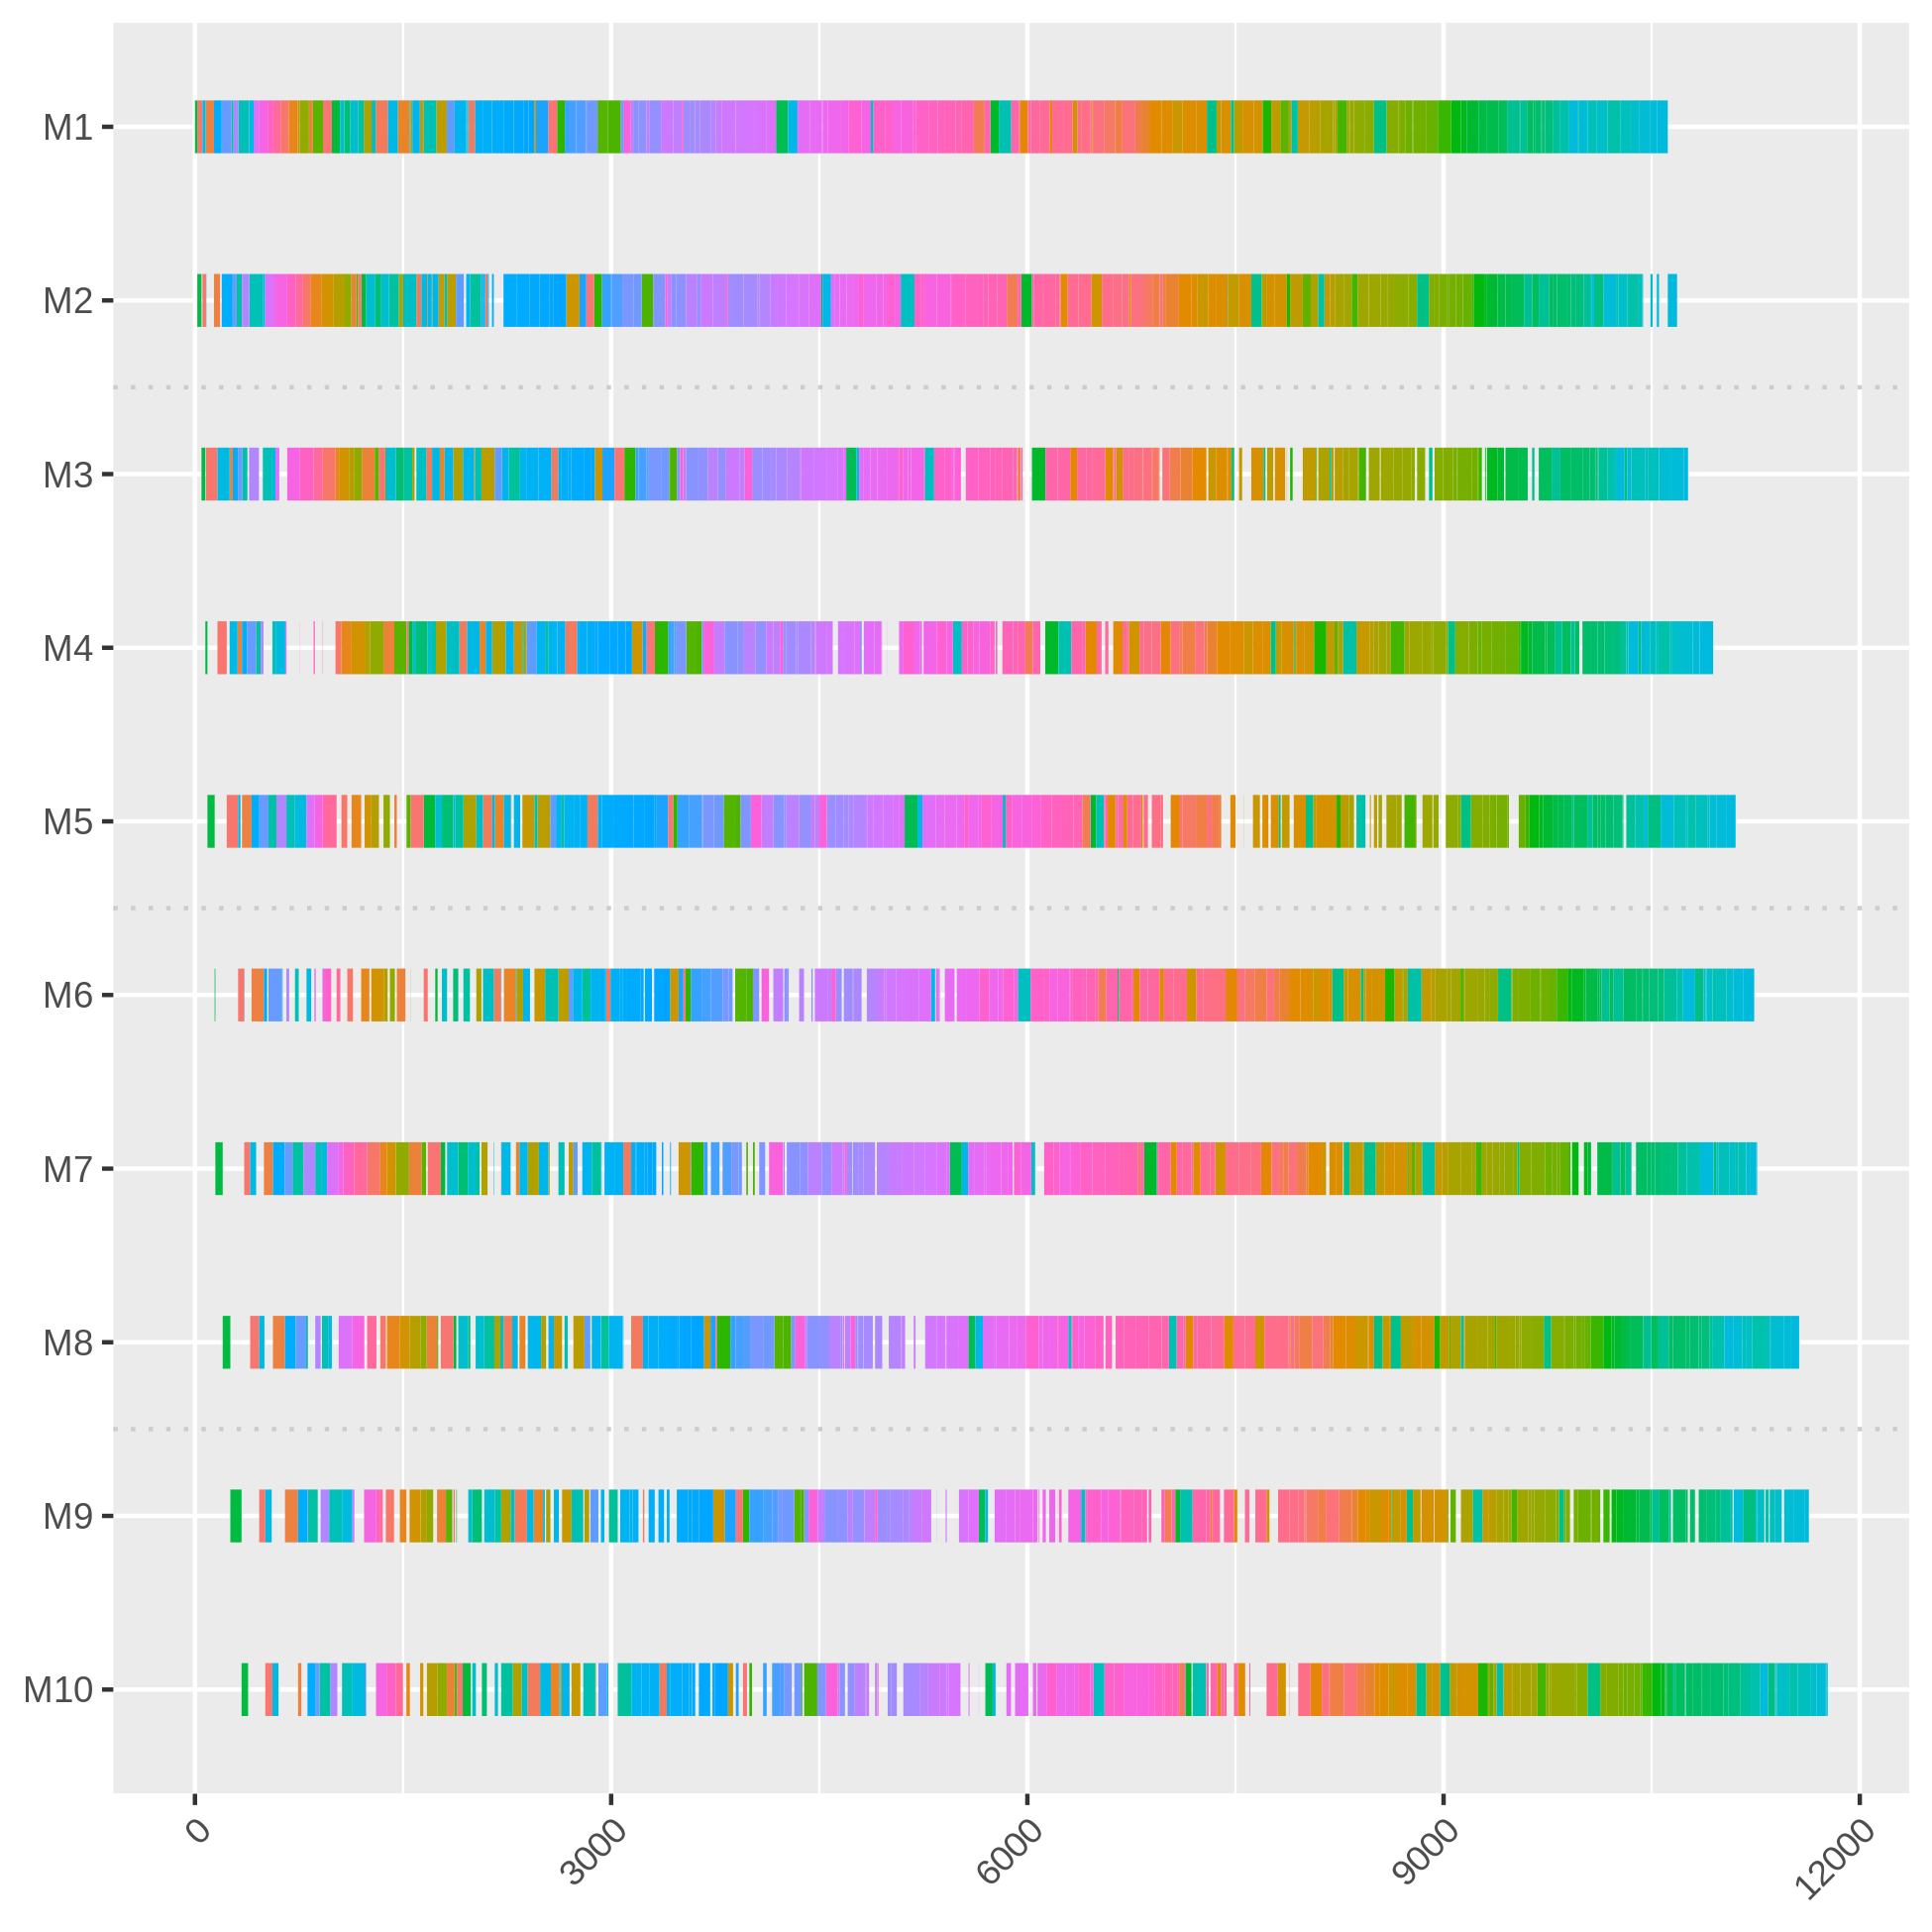
\includegraphics[width=\linewidth]{10_200_GC_1.png}
				\captionof{figure}{Gantt Chart for file 91.txt}
				
				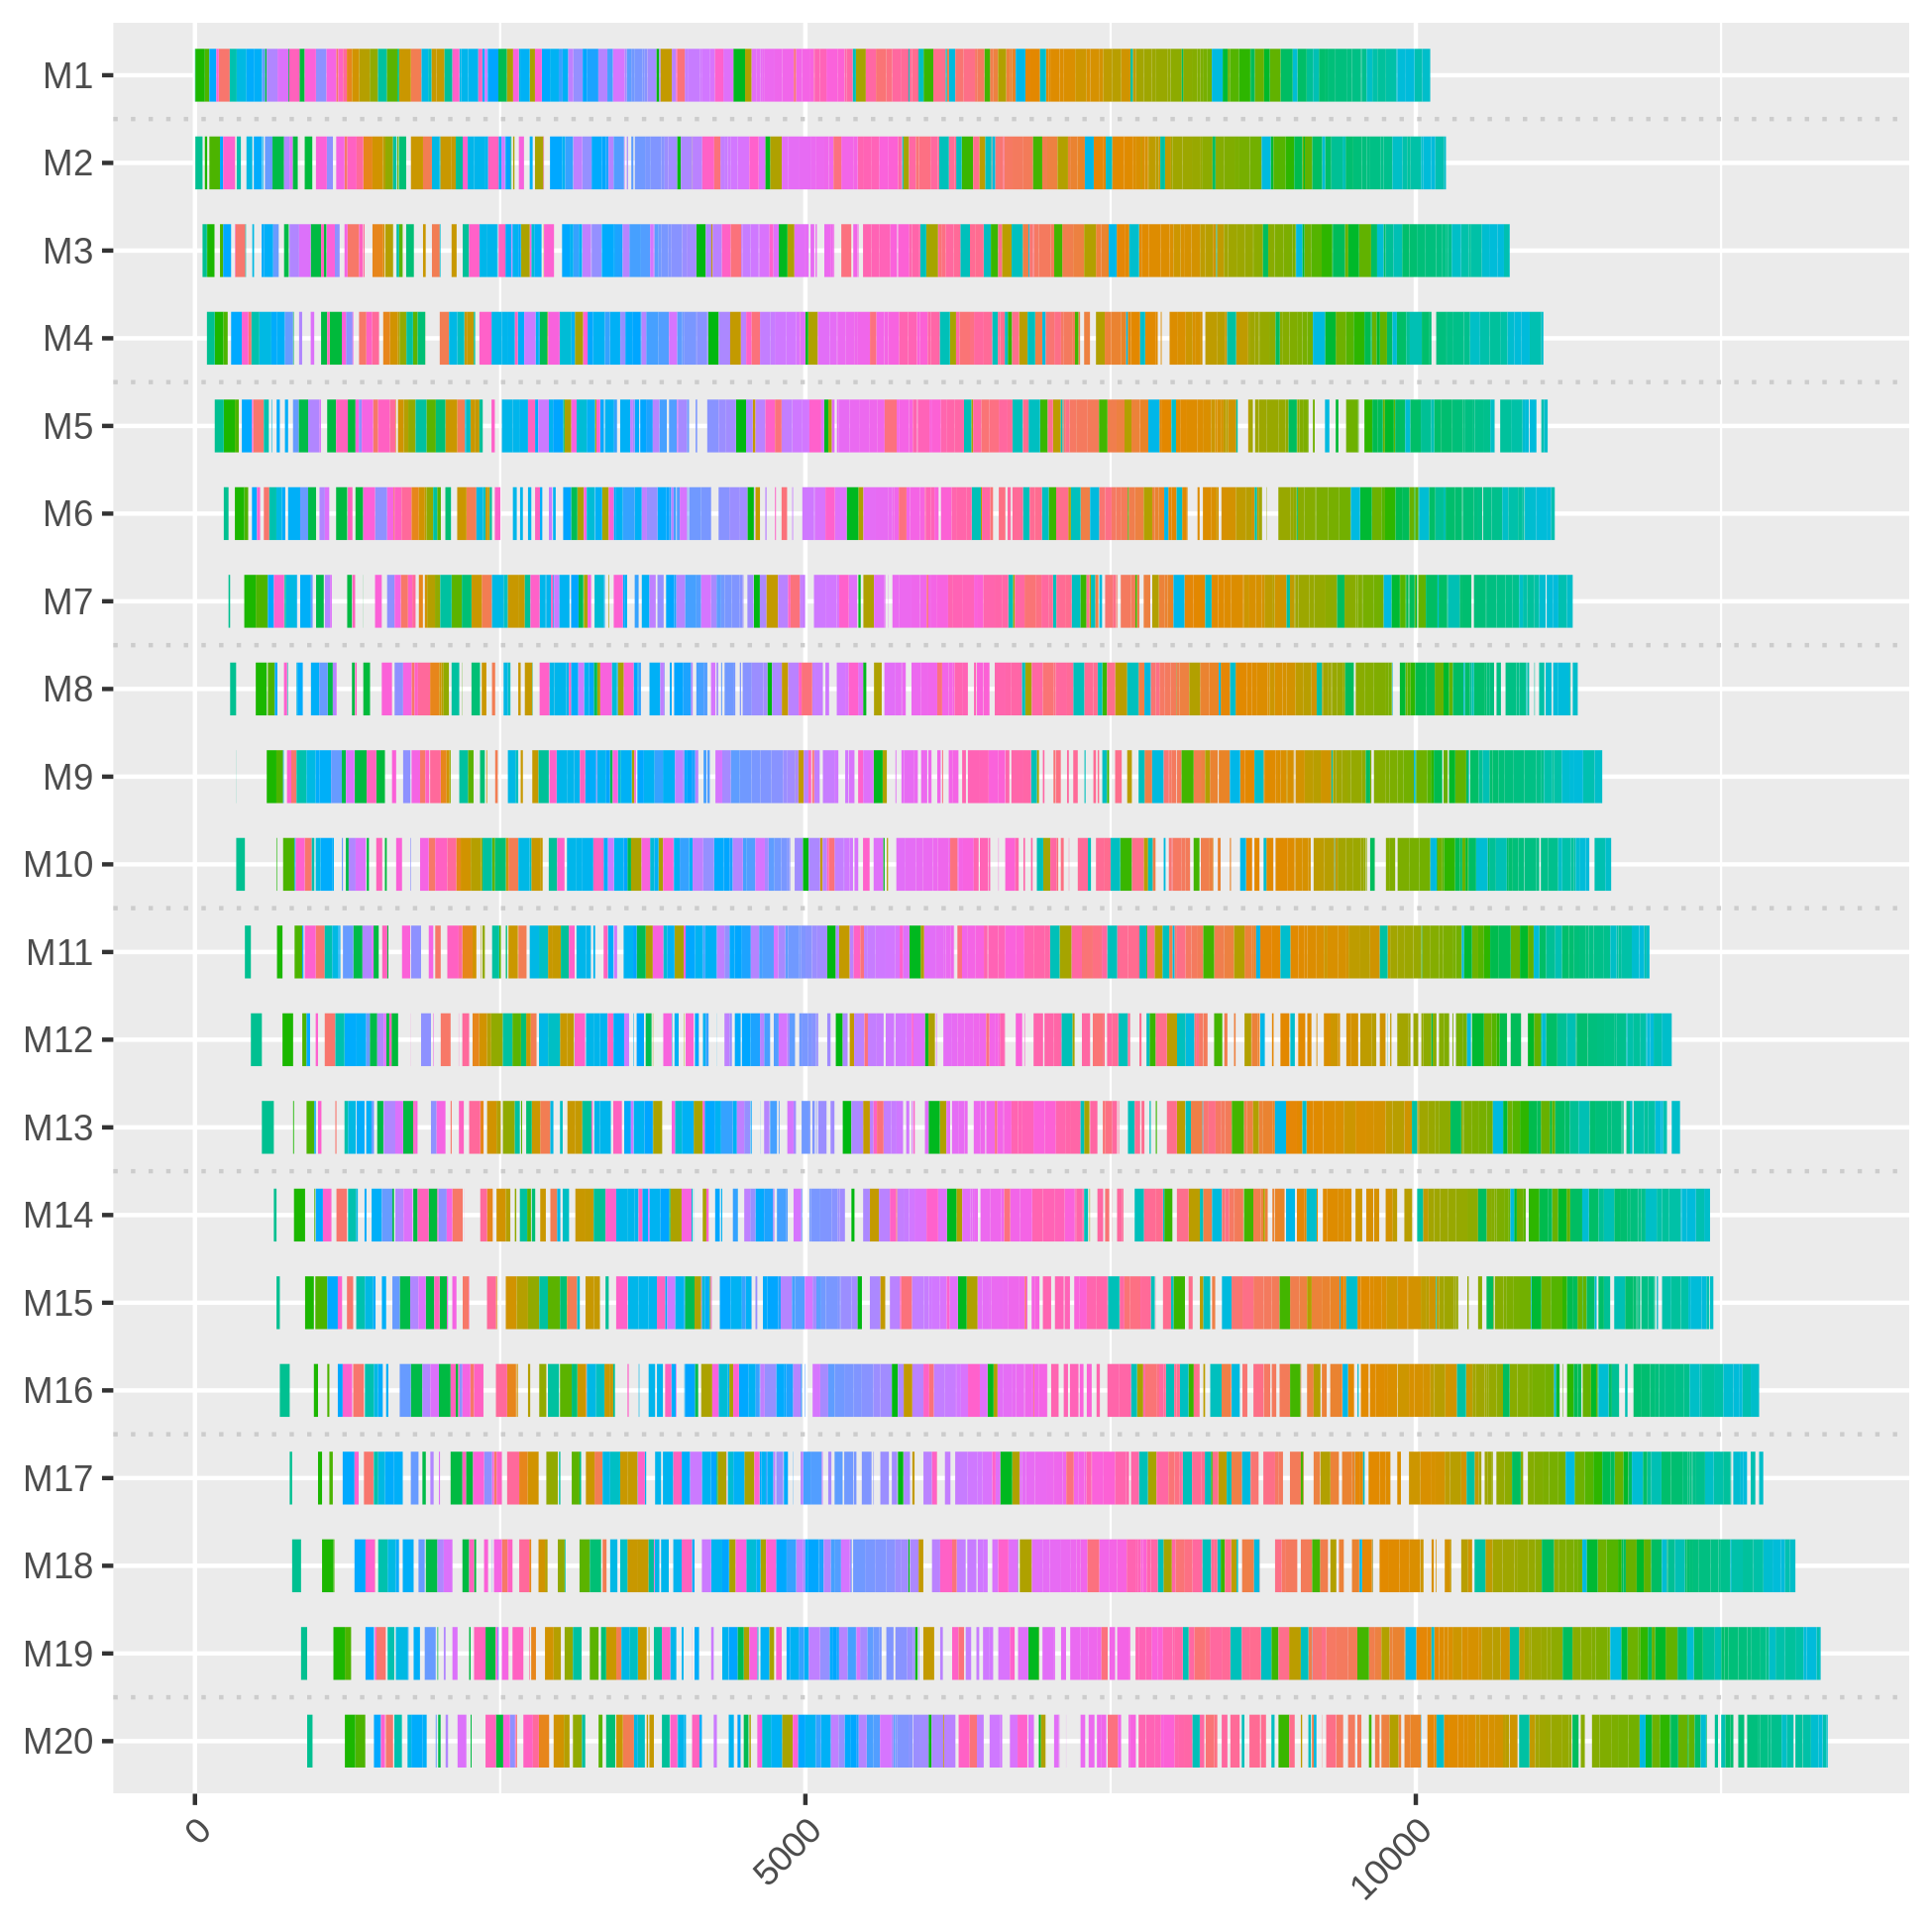
\includegraphics[width=\linewidth]{20_200_GC_1.png}
				\captionof{figure}{Gantt Chart for file 101.txt}
				
				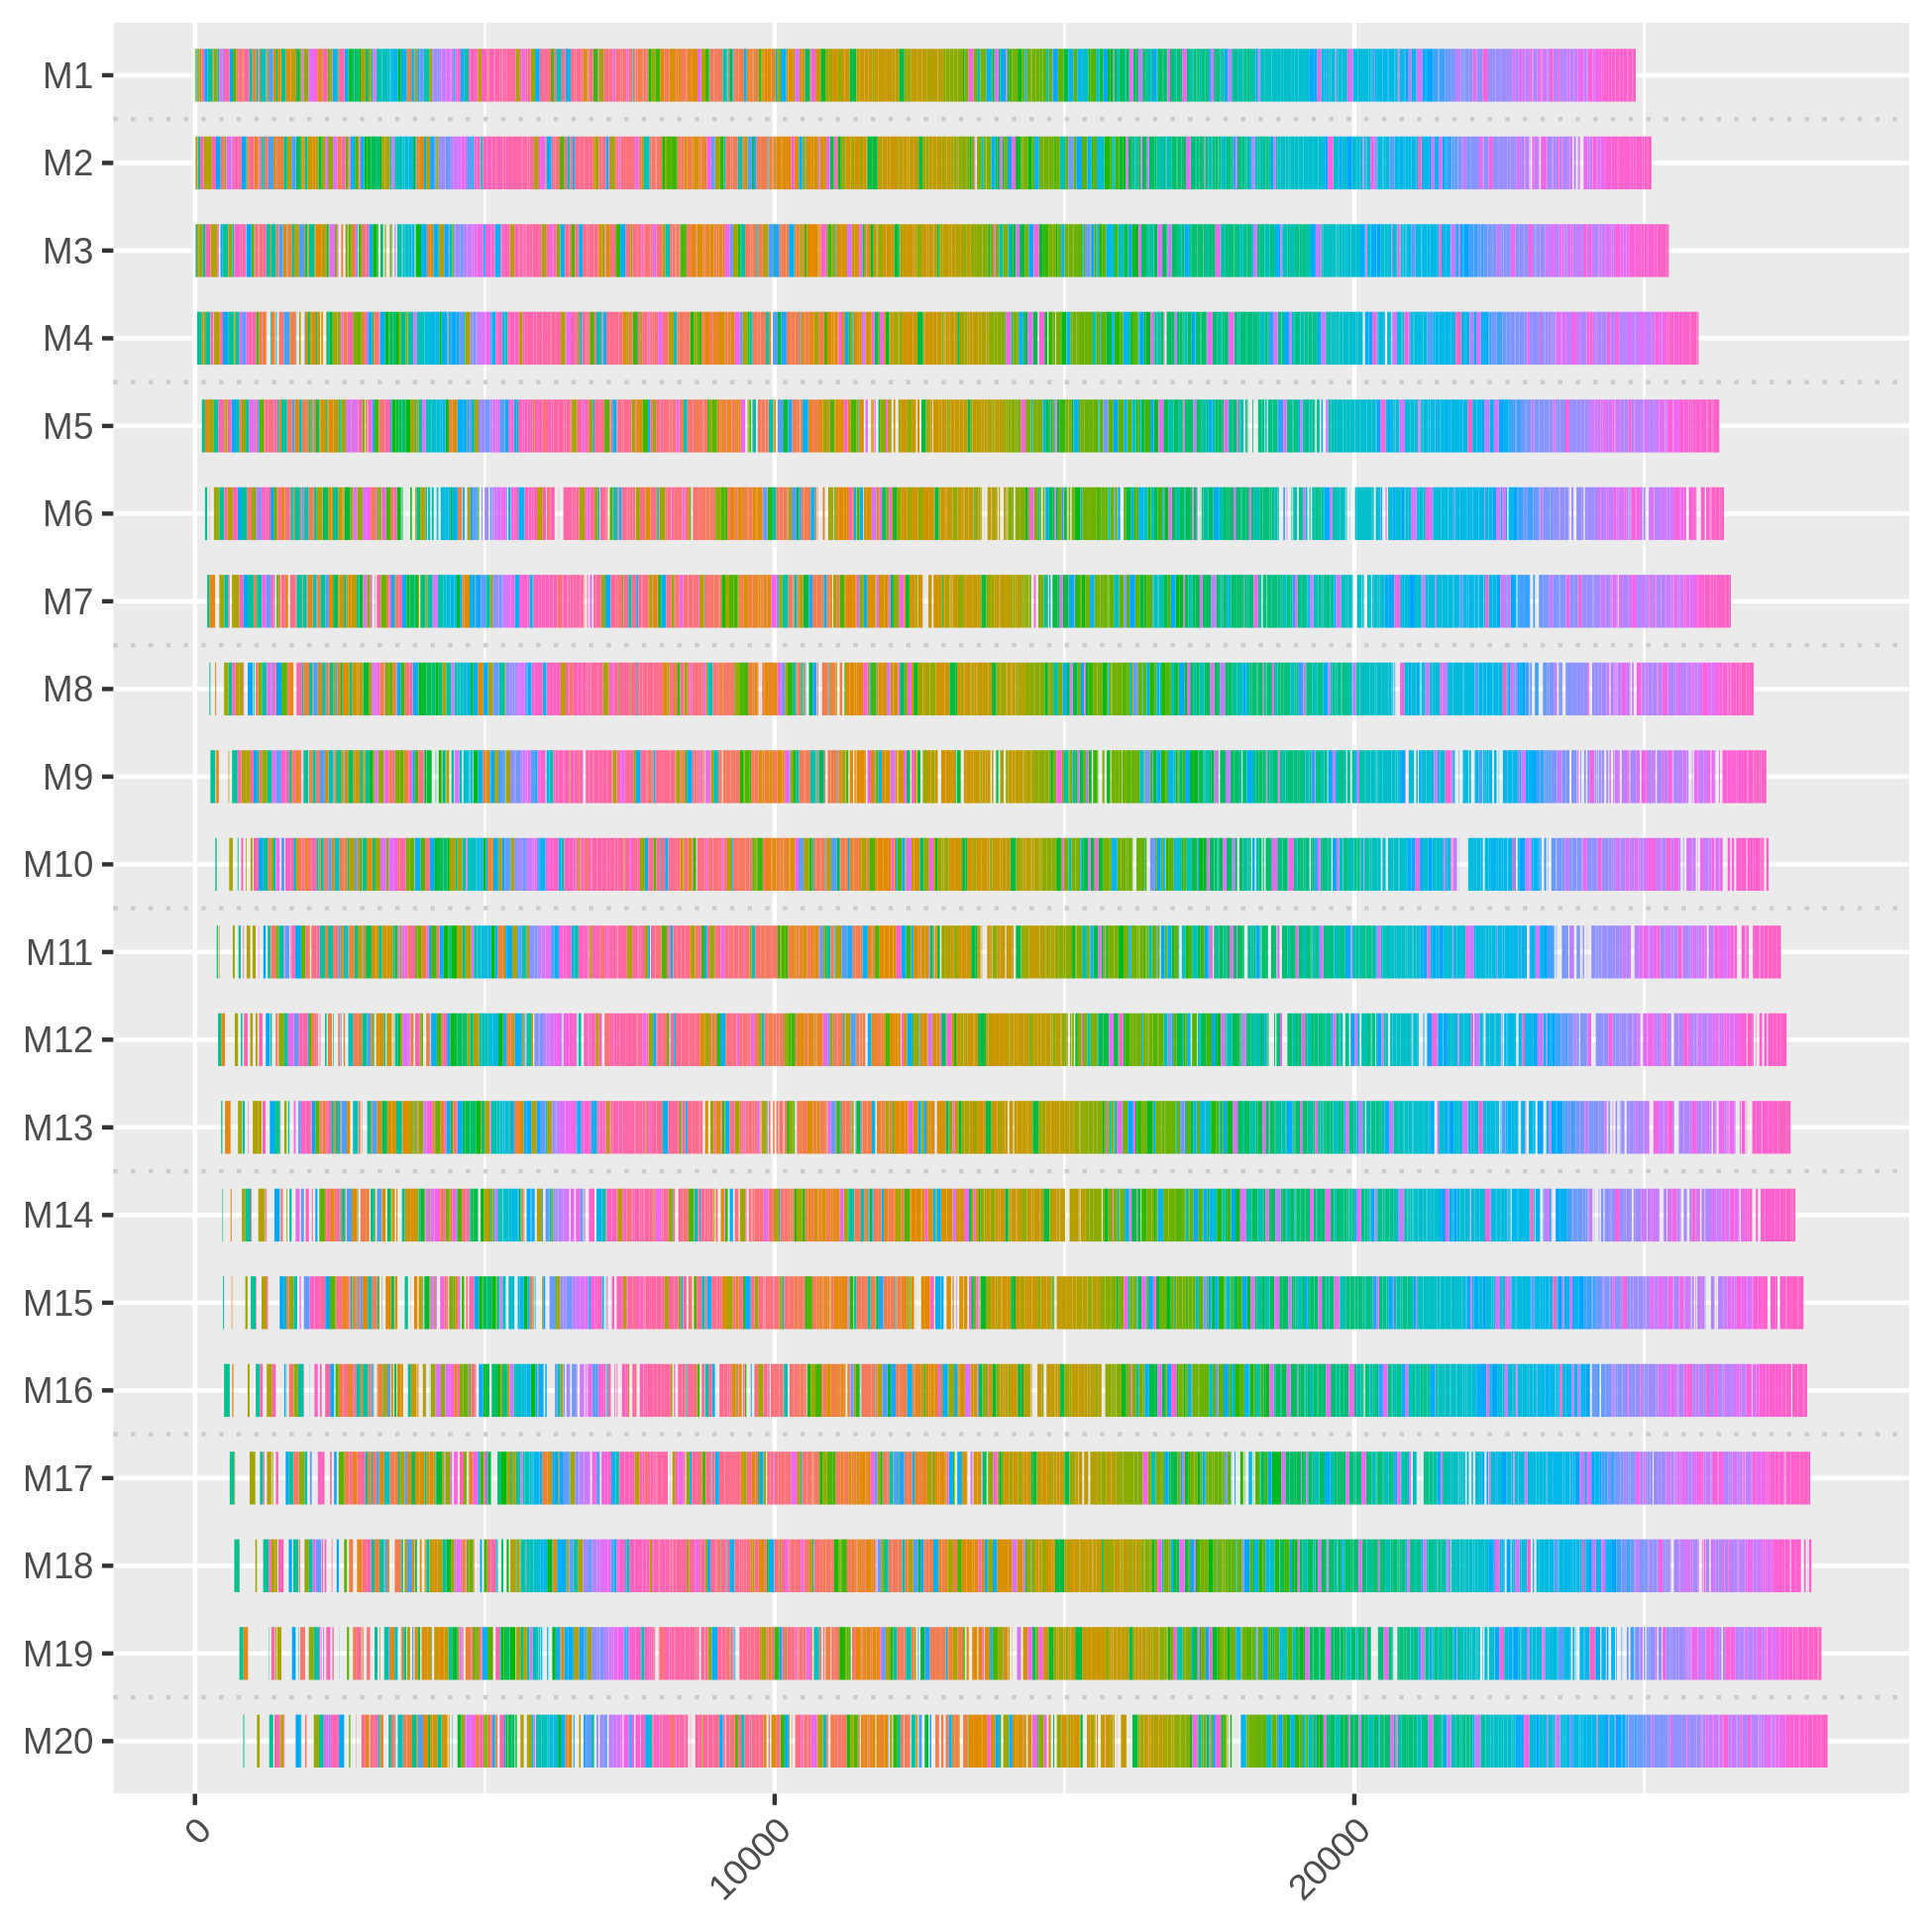
\includegraphics[width=\linewidth]{20_500_GC_1.png}
				\captionof{figure}{Gantt Chart for file 111.txt}
				
			\subsubsection{Results for Flow Shop Scheduling}
			\clearpage
					
					% latex table generated in R 3.6.0 by xtable 1.8-3 package
					% Fri May 31 14:47:46 2019
					\begin{table}[ht]
							\scalebox{0.9}{
								\begin{tabular}{rlrr}
									\hline
									& {\textbf{File.name}} & {\textbf{Best.makespan}} & {\textbf{\# func calls}} \\ 
									\hline
									{\textit{1}} & ../DataFiles/1.txt & 1324 & 558 \\ 
									{\textit{2}} & ../DataFiles/10.txt & 1250 & 562 \\ 
									{\textit{3}} & ../DataFiles/2.txt & 1396 & 566 \\ 
									{\textit{4}} & ../DataFiles/3.txt & 1197 & 565 \\ 
									{\textit{5}} & ../DataFiles/4.txt & 1449 & 569 \\ 
									{\textit{6}} & ../DataFiles/5.txt & 1360 & 568 \\ 
									{\textit{7}} & ../DataFiles/6.txt & 1347 & 569 \\ 
									{\textit{8}} & ../DataFiles/7.txt & 1286 & 562 \\ 
									{\textit{9}} & ../DataFiles/8.txt & 1380 & 565 \\ 
									{\textit{10}} & ../DataFiles/9.txt & 1353 & 567 \\ 
									{\textit{11}} & ../DataFiles/11.txt & 1714 & 564 \\ 
									{\textit{12}} & ../DataFiles/12.txt & 1806 & 567 \\ 
									{\textit{13}} & ../DataFiles/13.txt & 1684 & 563 \\ 
									{\textit{14}} & ../DataFiles/14.txt & 1606 & 570 \\ 
									{\textit{15}} & ../DataFiles/15.txt & 1638 & 569 \\ 
									{\textit{16}} & ../DataFiles/16.txt & 1624 & 569 \\ 
									{\textit{17}} & ../DataFiles/17.txt & 1611 & 566 \\ 
									{\textit{18}} & ../DataFiles/18.txt & 1786 & 565 \\ 
									{\textit{19}} & ../DataFiles/19.txt & 1748 & 570 \\ 
									{\textit{20}} & ../DataFiles/20.txt & 1827 & 565 \\ 
									{\textit{21}} & ../DataFiles/21.txt & 2502 & 570 \\ 
									{\textit{22}} & ../DataFiles/22.txt & 2392 & 567 \\ 
									{\textit{23}} & ../DataFiles/23.txt & 2532 & 566 \\ 
									{\textit{24}} & ../DataFiles/24.txt & 2461 & 567 \\ 
									{\textit{25}} & ../DataFiles/25.txt & 2537 & 562 \\ 
									{\textit{26}} & ../DataFiles/26.txt & 2436 & 565 \\ 
									{\textit{27}} & ../DataFiles/27.txt & 2464 & 569 \\ 
									{\textit{28}} & ../DataFiles/28.txt & 2392 & 567 \\ 
									{\textit{29}} & ../DataFiles/29.txt & 2486 & 568 \\ 
									{\textit{30}} & ../DataFiles/30.txt & 2394 & 568 \\ 
									{\textit{31}} & ../DataFiles/31.txt & 2859 & 3668 \\ 
									{\textit{32}} & ../DataFiles/32.txt & 2942 & 3645 \\ 
									{\textit{33}} & ../DataFiles/33.txt & 2743 & 3644 \\ 
									{\textit{34}} & ../DataFiles/34.txt & 2931 & 3664 \\ 
									{\textit{35}} & ../DataFiles/35.txt & 2980 & 3656 \\ 
									{\textit{36}} & ../DataFiles/36.txt & 2987 & 3650 \\ 
									{\textit{37}} & ../DataFiles/37.txt & 2845 & 3657 \\ 
									{\textit{38}} & ../DataFiles/38.txt & 2866 & 3647 \\ 
									{\textit{39}} & ../DataFiles/39.txt & 2653 & 3642 \\ 
									{\textit{40}} & ../DataFiles/40.txt & 2822 & 3597 \\ 
									{\textit{41}} & ../DataFiles/41.txt & 3408 & 3657 \\ 
									{\textit{42}} & ../DataFiles/42.txt & 3445 & 3665 \\ 
									{\textit{43}} & ../DataFiles/43.txt & 3253 & 3662 \\ 
									{\textit{44}} & ../DataFiles/44.txt & 3365 & 3665 \\ 
									{\textit{45}} & ../DataFiles/45.txt & 3396 & 3668 \\ 
									\hline
								\end{tabular}
							}
					\end{table}
				\clearpage
				\begin{table}[ht]
						\scalebox{0.9}{
							\begin{tabular}{rlrr}
								\hline
								& {\textbf{File.name}} & {\textbf{Best.makespan}} & {\textbf{\# func calls}} \\ 
								\hline
								{\textit{1}} & ../DataFiles/46.txt & 3365 & 3659 \\ 
								{\textit{2}} & ../DataFiles/47.txt & 3495 & 3656 \\ 
								{\textit{3}} & ../DataFiles/48.txt & 3309 & 3659 \\ 
								{\textit{4}} & ../DataFiles/49.txt & 3176 & 3664 \\ 
								{\textit{5}} & ../DataFiles/50.txt & 3476 & 3645 \\ 
								{\textit{6}} & ../DataFiles/51.txt & 4285 & 3663 \\ 
								{\textit{7}} & ../DataFiles/52.txt & 4172 & 3659 \\ 
								{\textit{8}} & ../DataFiles/53.txt & 4130 & 3649 \\ 
								{\textit{9}} & ../DataFiles/54.txt & 4225 & 3648 \\ 
								{\textit{10}} & ../DataFiles/55.txt & 4163 & 3659 \\ 
								{\textit{11}} & ../DataFiles/56.txt & 4228 & 3661 \\ 
								{\textit{12}} & ../DataFiles/57.txt & 4262 & 3655 \\ 
								{\textit{13}} & ../DataFiles/58.txt & 4213 & 3660 \\ 
								{\textit{14}} & ../DataFiles/59.txt & 4141 & 3648 \\ 
								{\textit{15}} & ../DataFiles/60.txt & 4218 & 3651 \\ 
								{\textit{16}} & ../DataFiles/61.txt & 5660 & 14801 \\ 
								{\textit{17}} & ../DataFiles/62.txt & 5345 & 14799 \\ 
								{\textit{18}} & ../DataFiles/63.txt & 5455 & 14801 \\ 
								{\textit{19}} & ../DataFiles/64.txt & 5205 & 14794 \\ 
								{\textit{20}} & ../DataFiles/65.txt & 5486 & 14794 \\ 
								{\textit{21}} & ../DataFiles/66.txt & 5314 & 14796 \\ 
								{\textit{22}} & ../DataFiles/67.txt & 5530 & 14795 \\ 
								{\textit{23}} & ../DataFiles/68.txt & 5179 & 14813 \\ 
								{\textit{24}} & ../DataFiles/69.txt & 5518 & 14782 \\ 
								{\textit{25}} & ../DataFiles/70.txt & 5459 & 14810 \\ 
								{\textit{26}} & ../DataFiles/71.txt & 6285 & 14792 \\ 
								{\textit{27}} & ../DataFiles/72.txt & 5822 & 14815 \\ 
								{\textit{28}} & ../DataFiles/73.txt & 6178 & 14803 \\ 
								{\textit{29}} & ../DataFiles/74.txt & 6311 & 14817 \\ 
								{\textit{30}} & ../DataFiles/75.txt & 5956 & 14812 \\ 
								{\textit{31}} & ../DataFiles/76.txt & 5774 & 14824 \\ 
								{\textit{32}} & ../DataFiles/77.txt & 5869 & 14815 \\ 
								{\textit{33}} & ../DataFiles/78.txt & 6105 & 14799 \\ 
								{\textit{34}} & ../DataFiles/79.txt & 6209 & 14801 \\ 
								{\textit{35}} & ../DataFiles/80.txt & 6273 & 14801 \\ 
								{\textit{36}} & ../DataFiles/81.txt & 6954 & 14749 \\ 
								{\textit{37}} & ../DataFiles/82.txt & 7138 & 14733 \\ 
								{\textit{38}} & ../DataFiles/83.txt & 6978 & 14740 \\ 
								{\textit{39}} & ../DataFiles/84.txt & 6882 & 14717 \\ 
								{\textit{40}} & ../DataFiles/85.txt & 7168 & 14733 \\ 
								{\textit{41}} & ../DataFiles/86.txt & 7283 & 14724 \\ 
								{\textit{42}} & ../DataFiles/87.txt & 6957 & 14749 \\ 
								{\textit{43}} & ../DataFiles/88.txt & 7350 & 14702 \\ 
								{\textit{44}} & ../DataFiles/89.txt & 7098 & 14723 \\ 
								{\textit{45}} & ../DataFiles/90.txt & 7217 & 14661 \\ 
								{\textit{46}} & ../DataFiles/100.txt & 11336 & 59401 \\ 
								\hline
							\end{tabular}
						}
				\end{table}
				\clearpage
				\begin{table}[ht]
						\scalebox{0.9}{
							\begin{tabular}{rlrr}
								\hline
								& {\textbf{File.name}} & {\textbf{Best.makespan}} & {\textbf{\# func calls}} \\ 
								\hline
								{\textit{1}} & ../DataFiles/91.txt & 11542 & 59416 \\ 
								{\textit{2}} & ../DataFiles/92.txt & 11290 & 59441 \\ 
								{\textit{3}} & ../DataFiles/93.txt & 11731 & 59253 \\ 
								{\textit{4}} & ../DataFiles/94.txt & 11222 & 59446 \\ 
								{\textit{5}} & ../DataFiles/95.txt & 11217 & 59494 \\ 
								{\textit{6}} & ../DataFiles/96.txt & 11166 & 59382 \\ 
								{\textit{7}} & ../DataFiles/97.txt & 11302 & 59553 \\ 
								{\textit{8}} & ../DataFiles/98.txt & 11465 & 59313 \\ 
								{\textit{9}} & ../DataFiles/99.txt & 11178 & 59426 \\ 
								{\textit{10}} & ../DataFiles/101.txt & 12338 & 58906 \\ 
								{\textit{11}} & ../DataFiles/102.txt & 12498 & 59106 \\ 
								{\textit{12}} & ../DataFiles/103.txt & 12678 & 59219 \\ 
								{\textit{13}} & ../DataFiles/104.txt & 12417 & 59099 \\ 
								{\textit{14}} & ../DataFiles/105.txt & 12501 & 58971 \\ 
								{\textit{15}} & ../DataFiles/106.txt & 12356 & 58916 \\ 
								{\textit{16}} & ../DataFiles/107.txt & 12658 & 58986 \\ 
								{\textit{17}} & ../DataFiles/108.txt & 12678 & 59048 \\ 
								{\textit{18}} & ../DataFiles/109.txt & 12465 & 59170 \\ 
								{\textit{19}} & ../DataFiles/110.txt & 12498 & 59202 \\ 
								{\textit{20}} & ../DataFiles/111.txt & 28166 & 371362 \\ 
								{\textit{21}} & ../DataFiles/112.txt & 28615 & 371897 \\ 
								{\textit{22}} & ../DataFiles/113.txt & 28151 & 371500 \\ 
								{\textit{23}} & ../DataFiles/114.txt & 28286 & 371772 \\ 
								{\textit{24}} & ../DataFiles/115.txt & 28567 & 371442 \\ 
								{\textit{25}} & ../DataFiles/116.txt & 28718 & 371436 \\ 
								{\textit{26}} & ../DataFiles/117.txt & 28195 & 371245 \\ 
								{\textit{27}} & ../DataFiles/118.txt & 28803 & 370891 \\ 
								{\textit{28}} & ../DataFiles/119.txt & 27873 & 371911 \\ 
								{\textit{29}} & ../DataFiles/120.txt & 28385 & 371341 \\ 
								\hline
							\end{tabular}
						
						}
					\caption{Results for Flow Shop Scheduling}
				\end{table}
			
				\subsubsection{Analysis}
					As seen from table1 above, both the makespan and the number of function calls increases as the number of machines or the number of jobs increases. The table also shows that the best makespan found are not really close to what is reported on Taillard website. For example the table shows that the best makespan found for file 54.txt is 3723
			
			
				\subsection{Flow Shop Scheduling With Blocking}
				\subsubsection{Gantt Charts}
					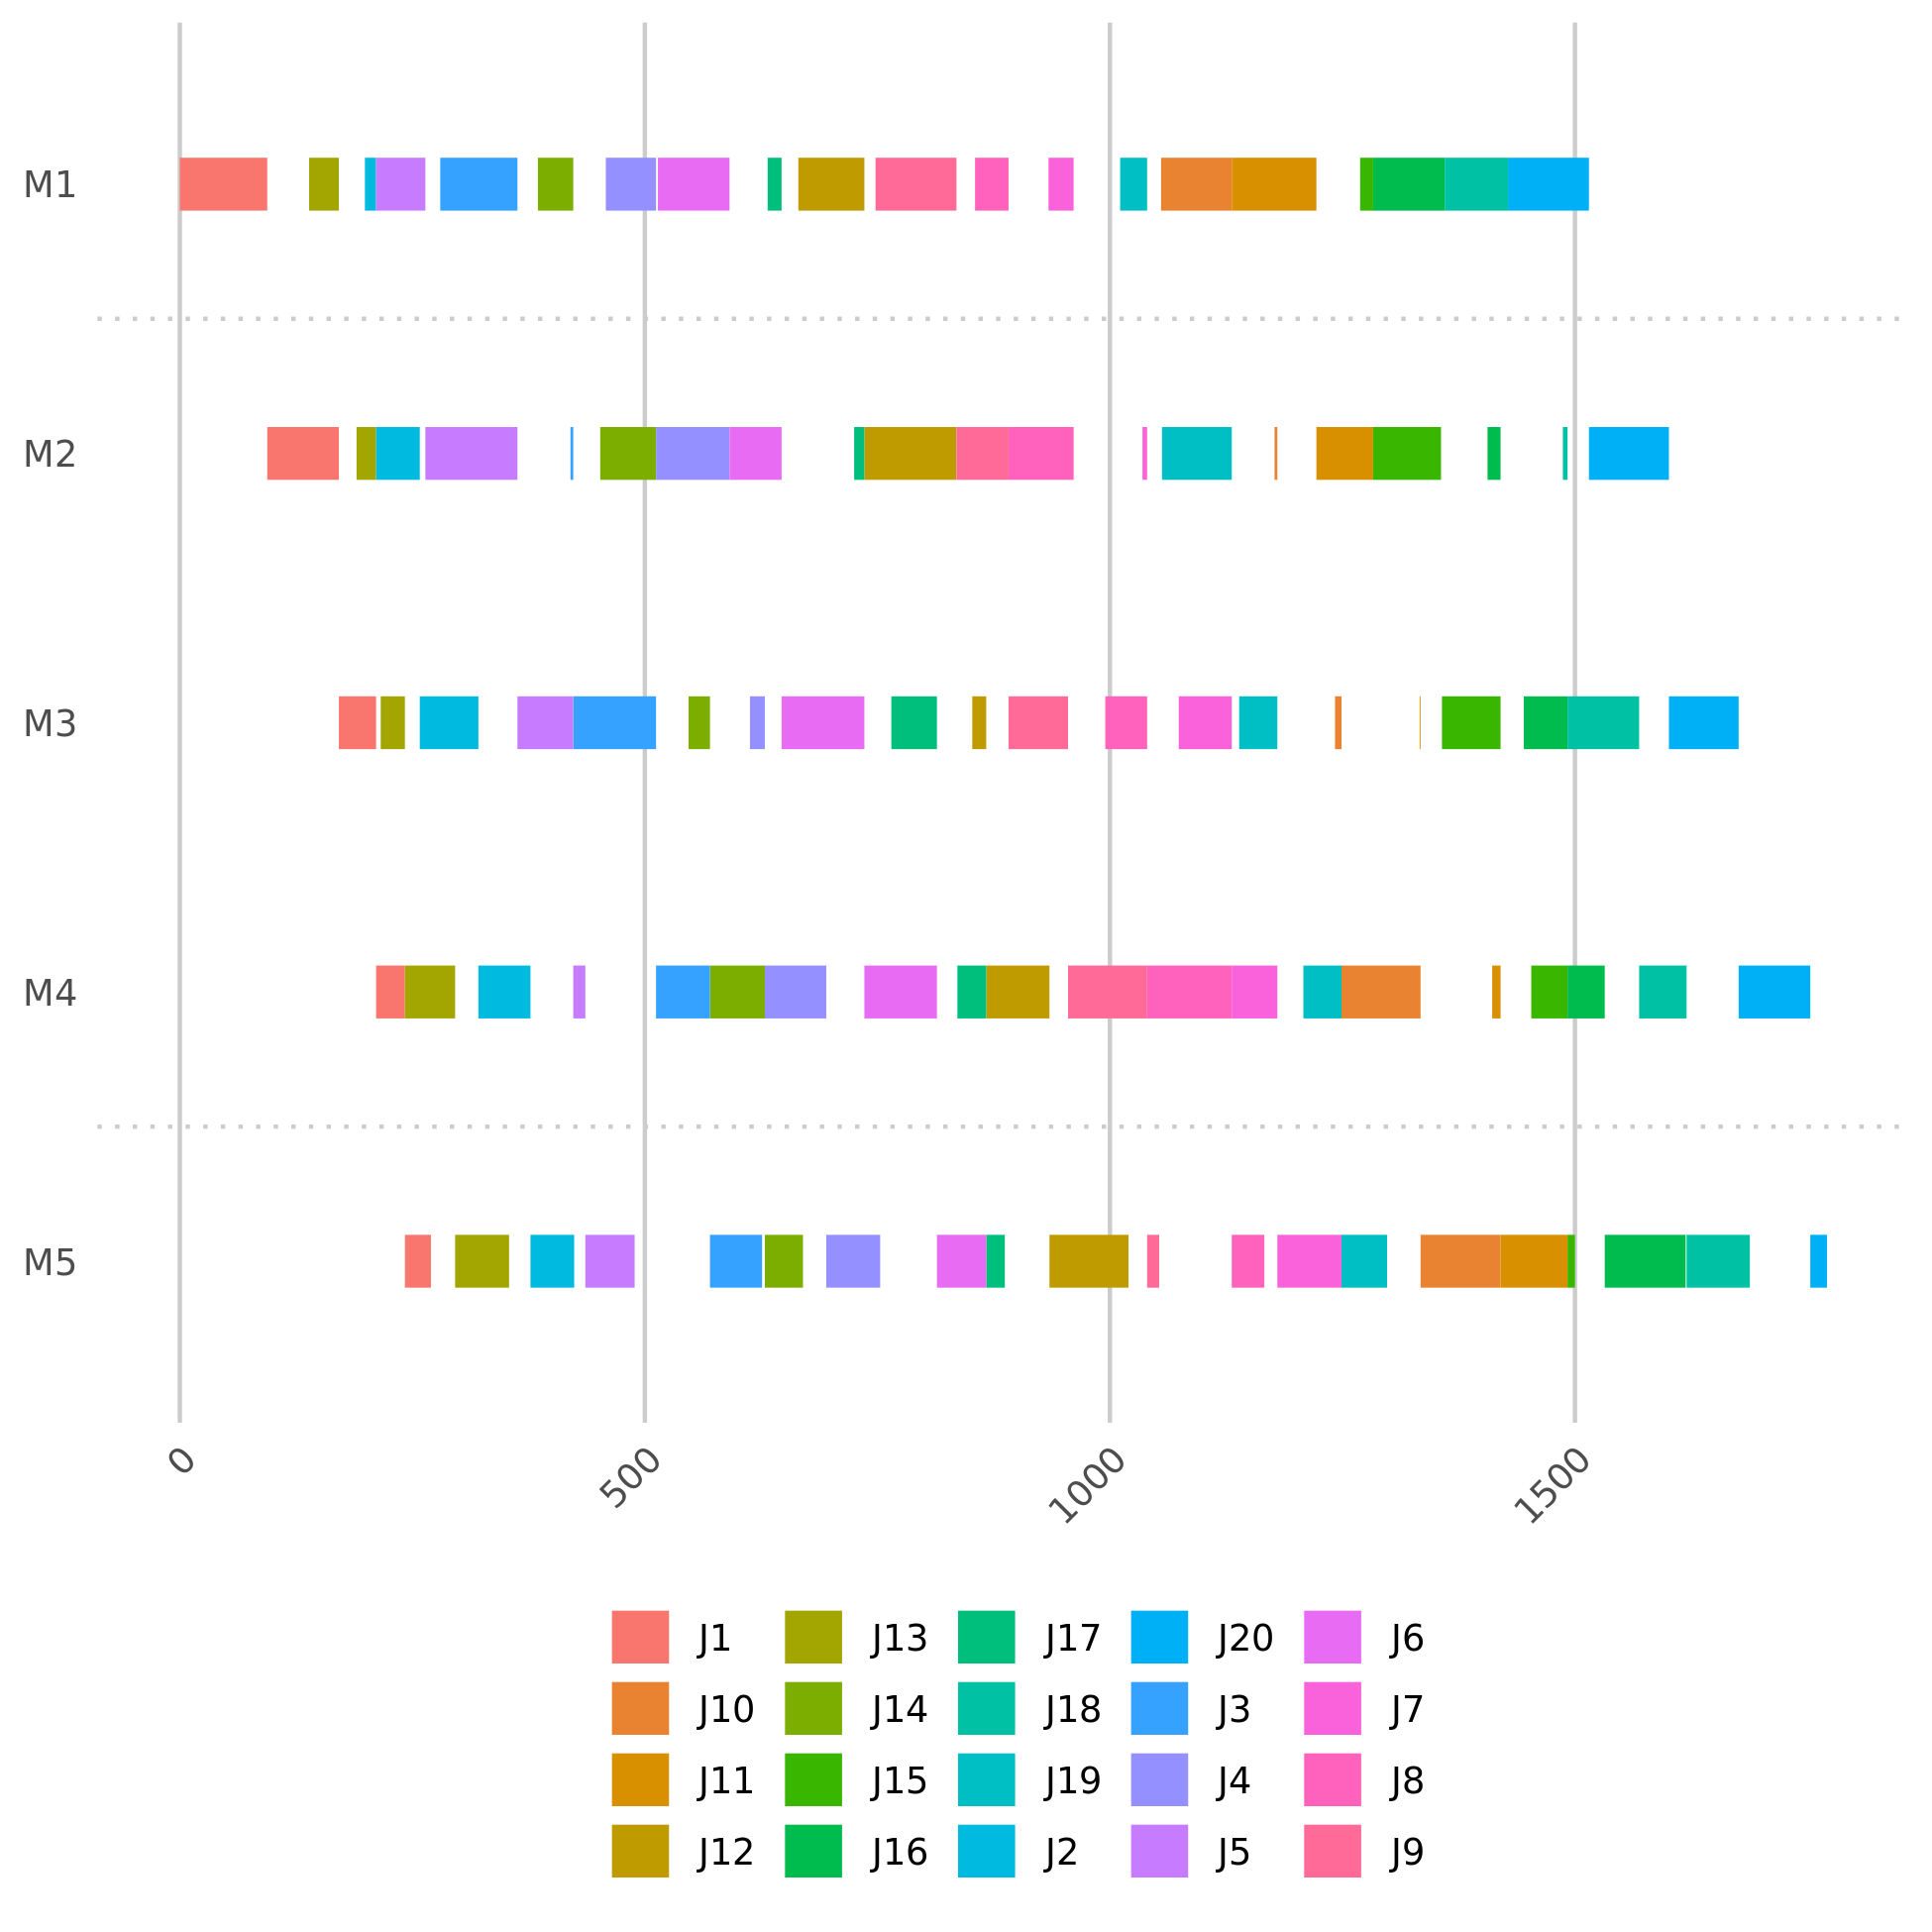
\includegraphics[width=\linewidth]{5_20_GC_2.png}
					\captionof{figure}{Gantt Chart for file 1.txt}
					
					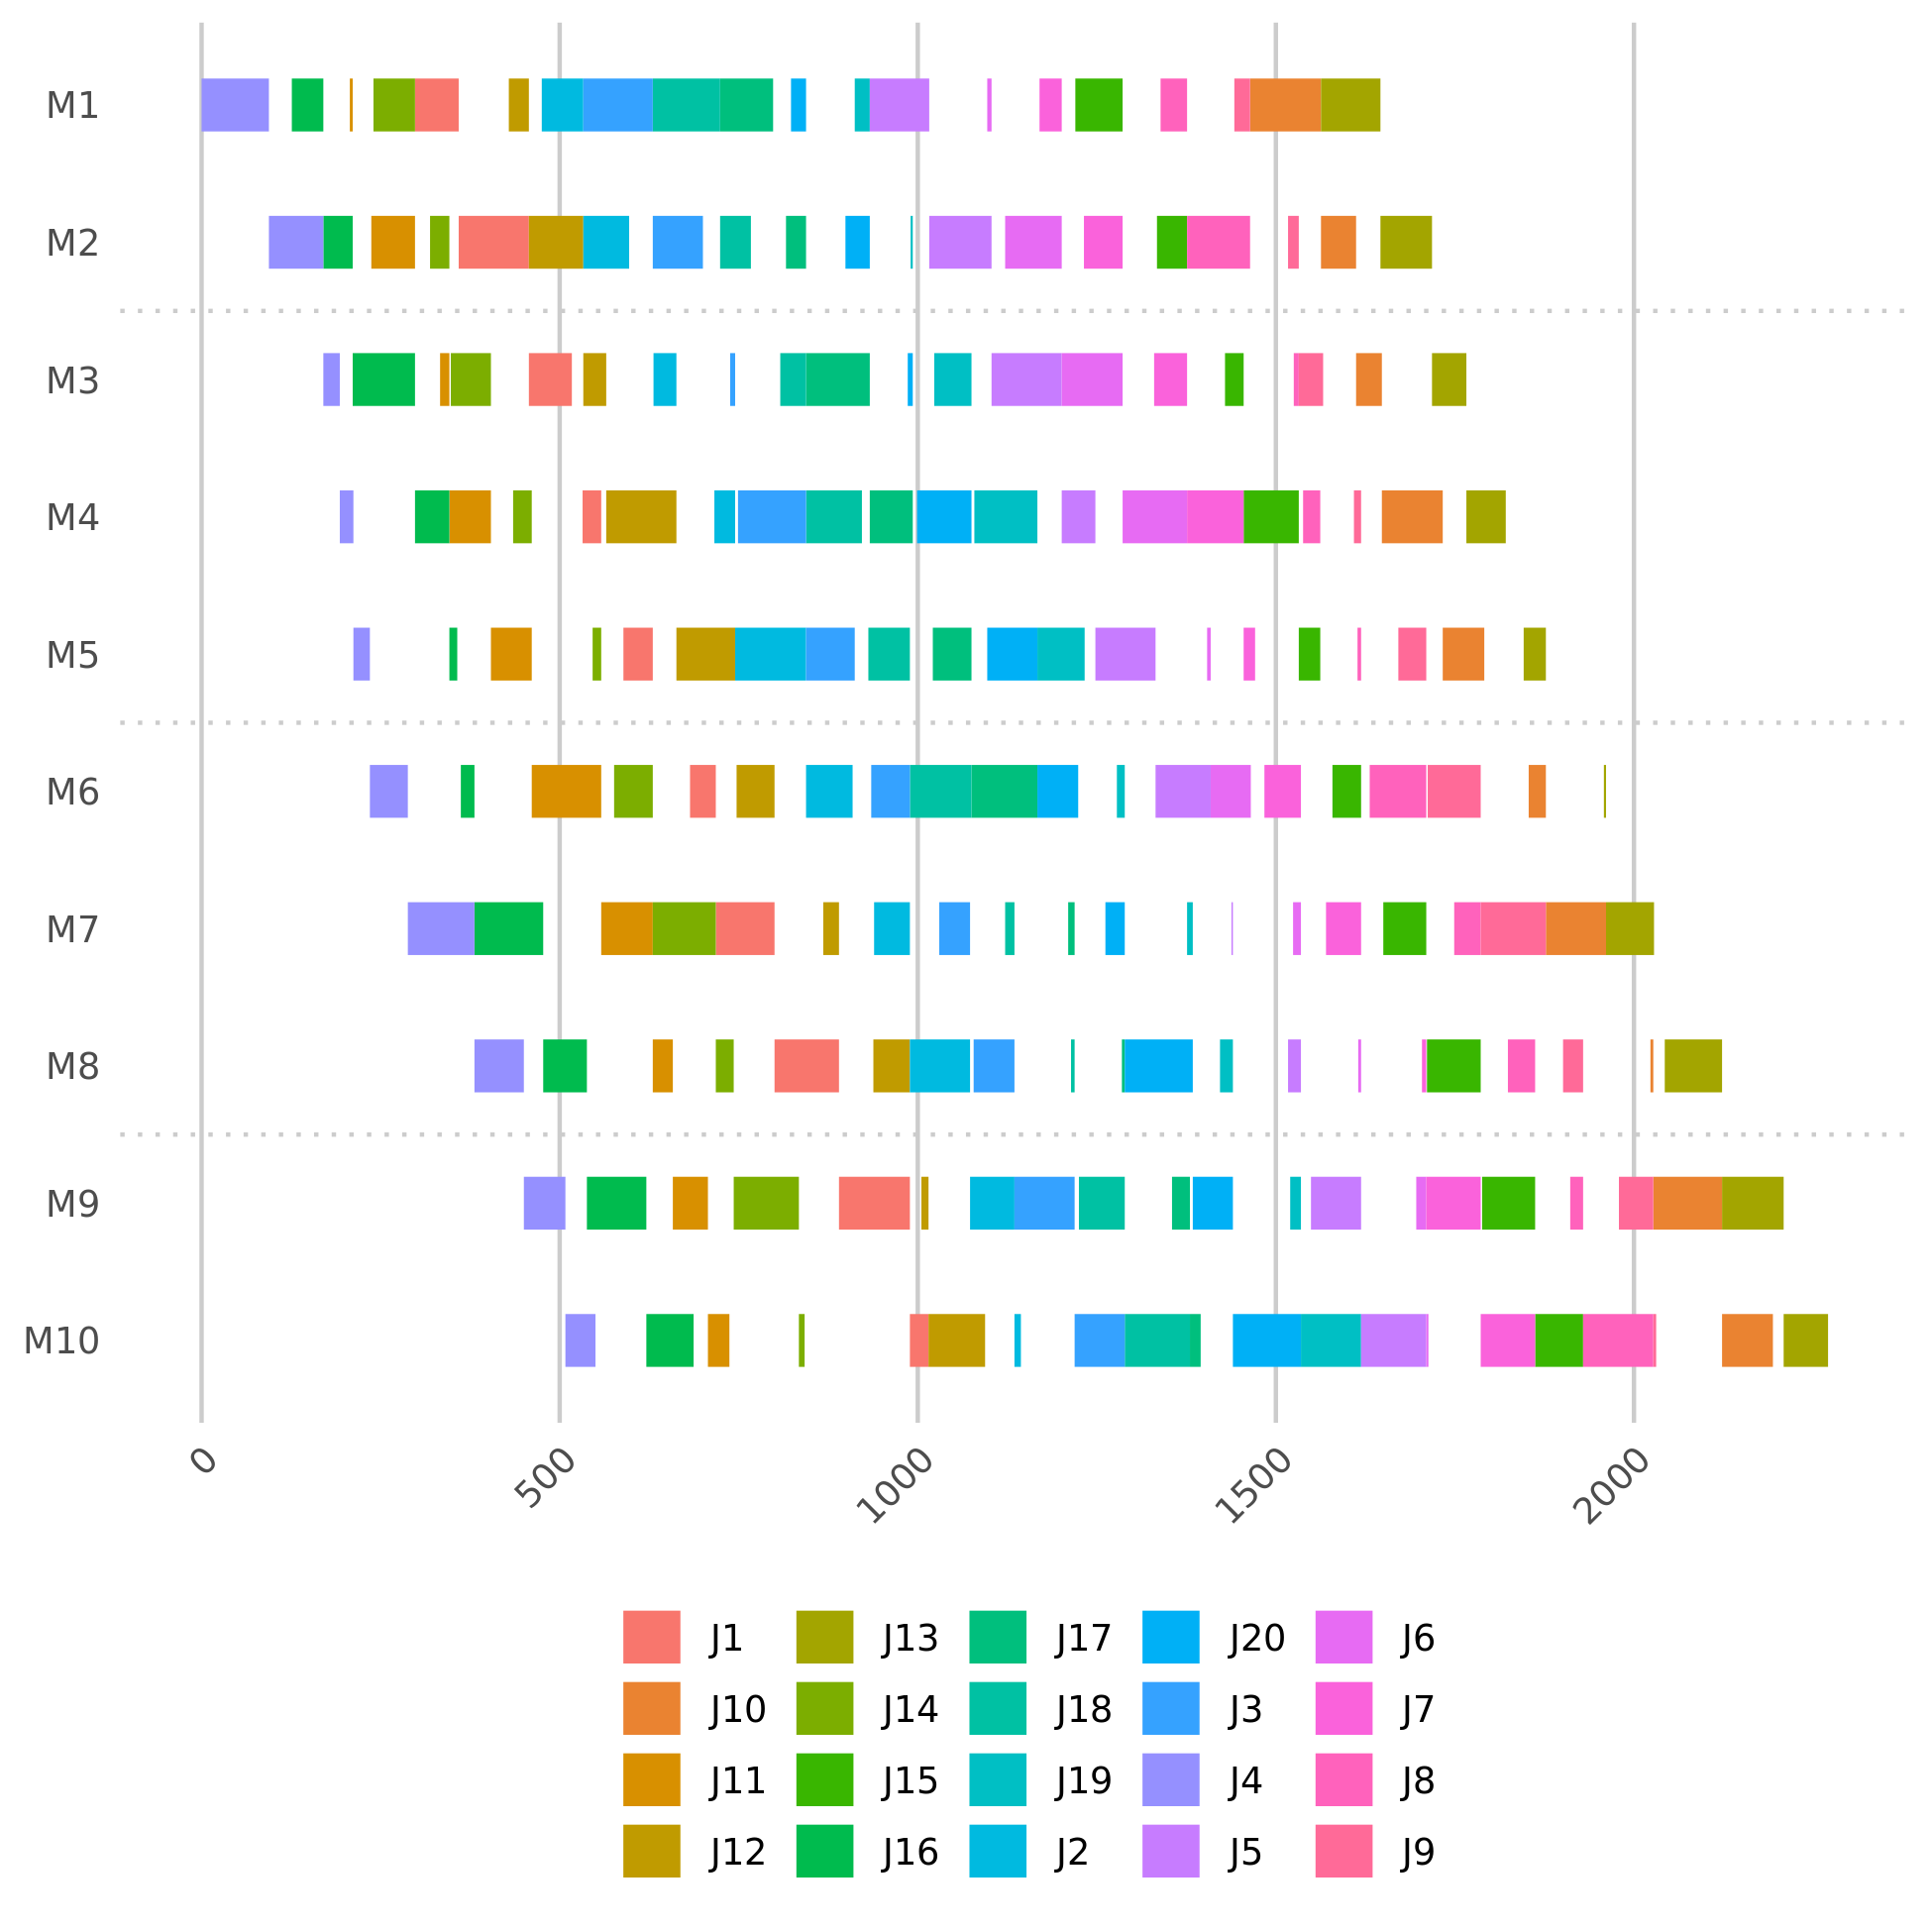
\includegraphics[width=\linewidth]{10_20_GC_2.png}
					\captionof{figure}{Gantt Chart for file 11.txt}
					
					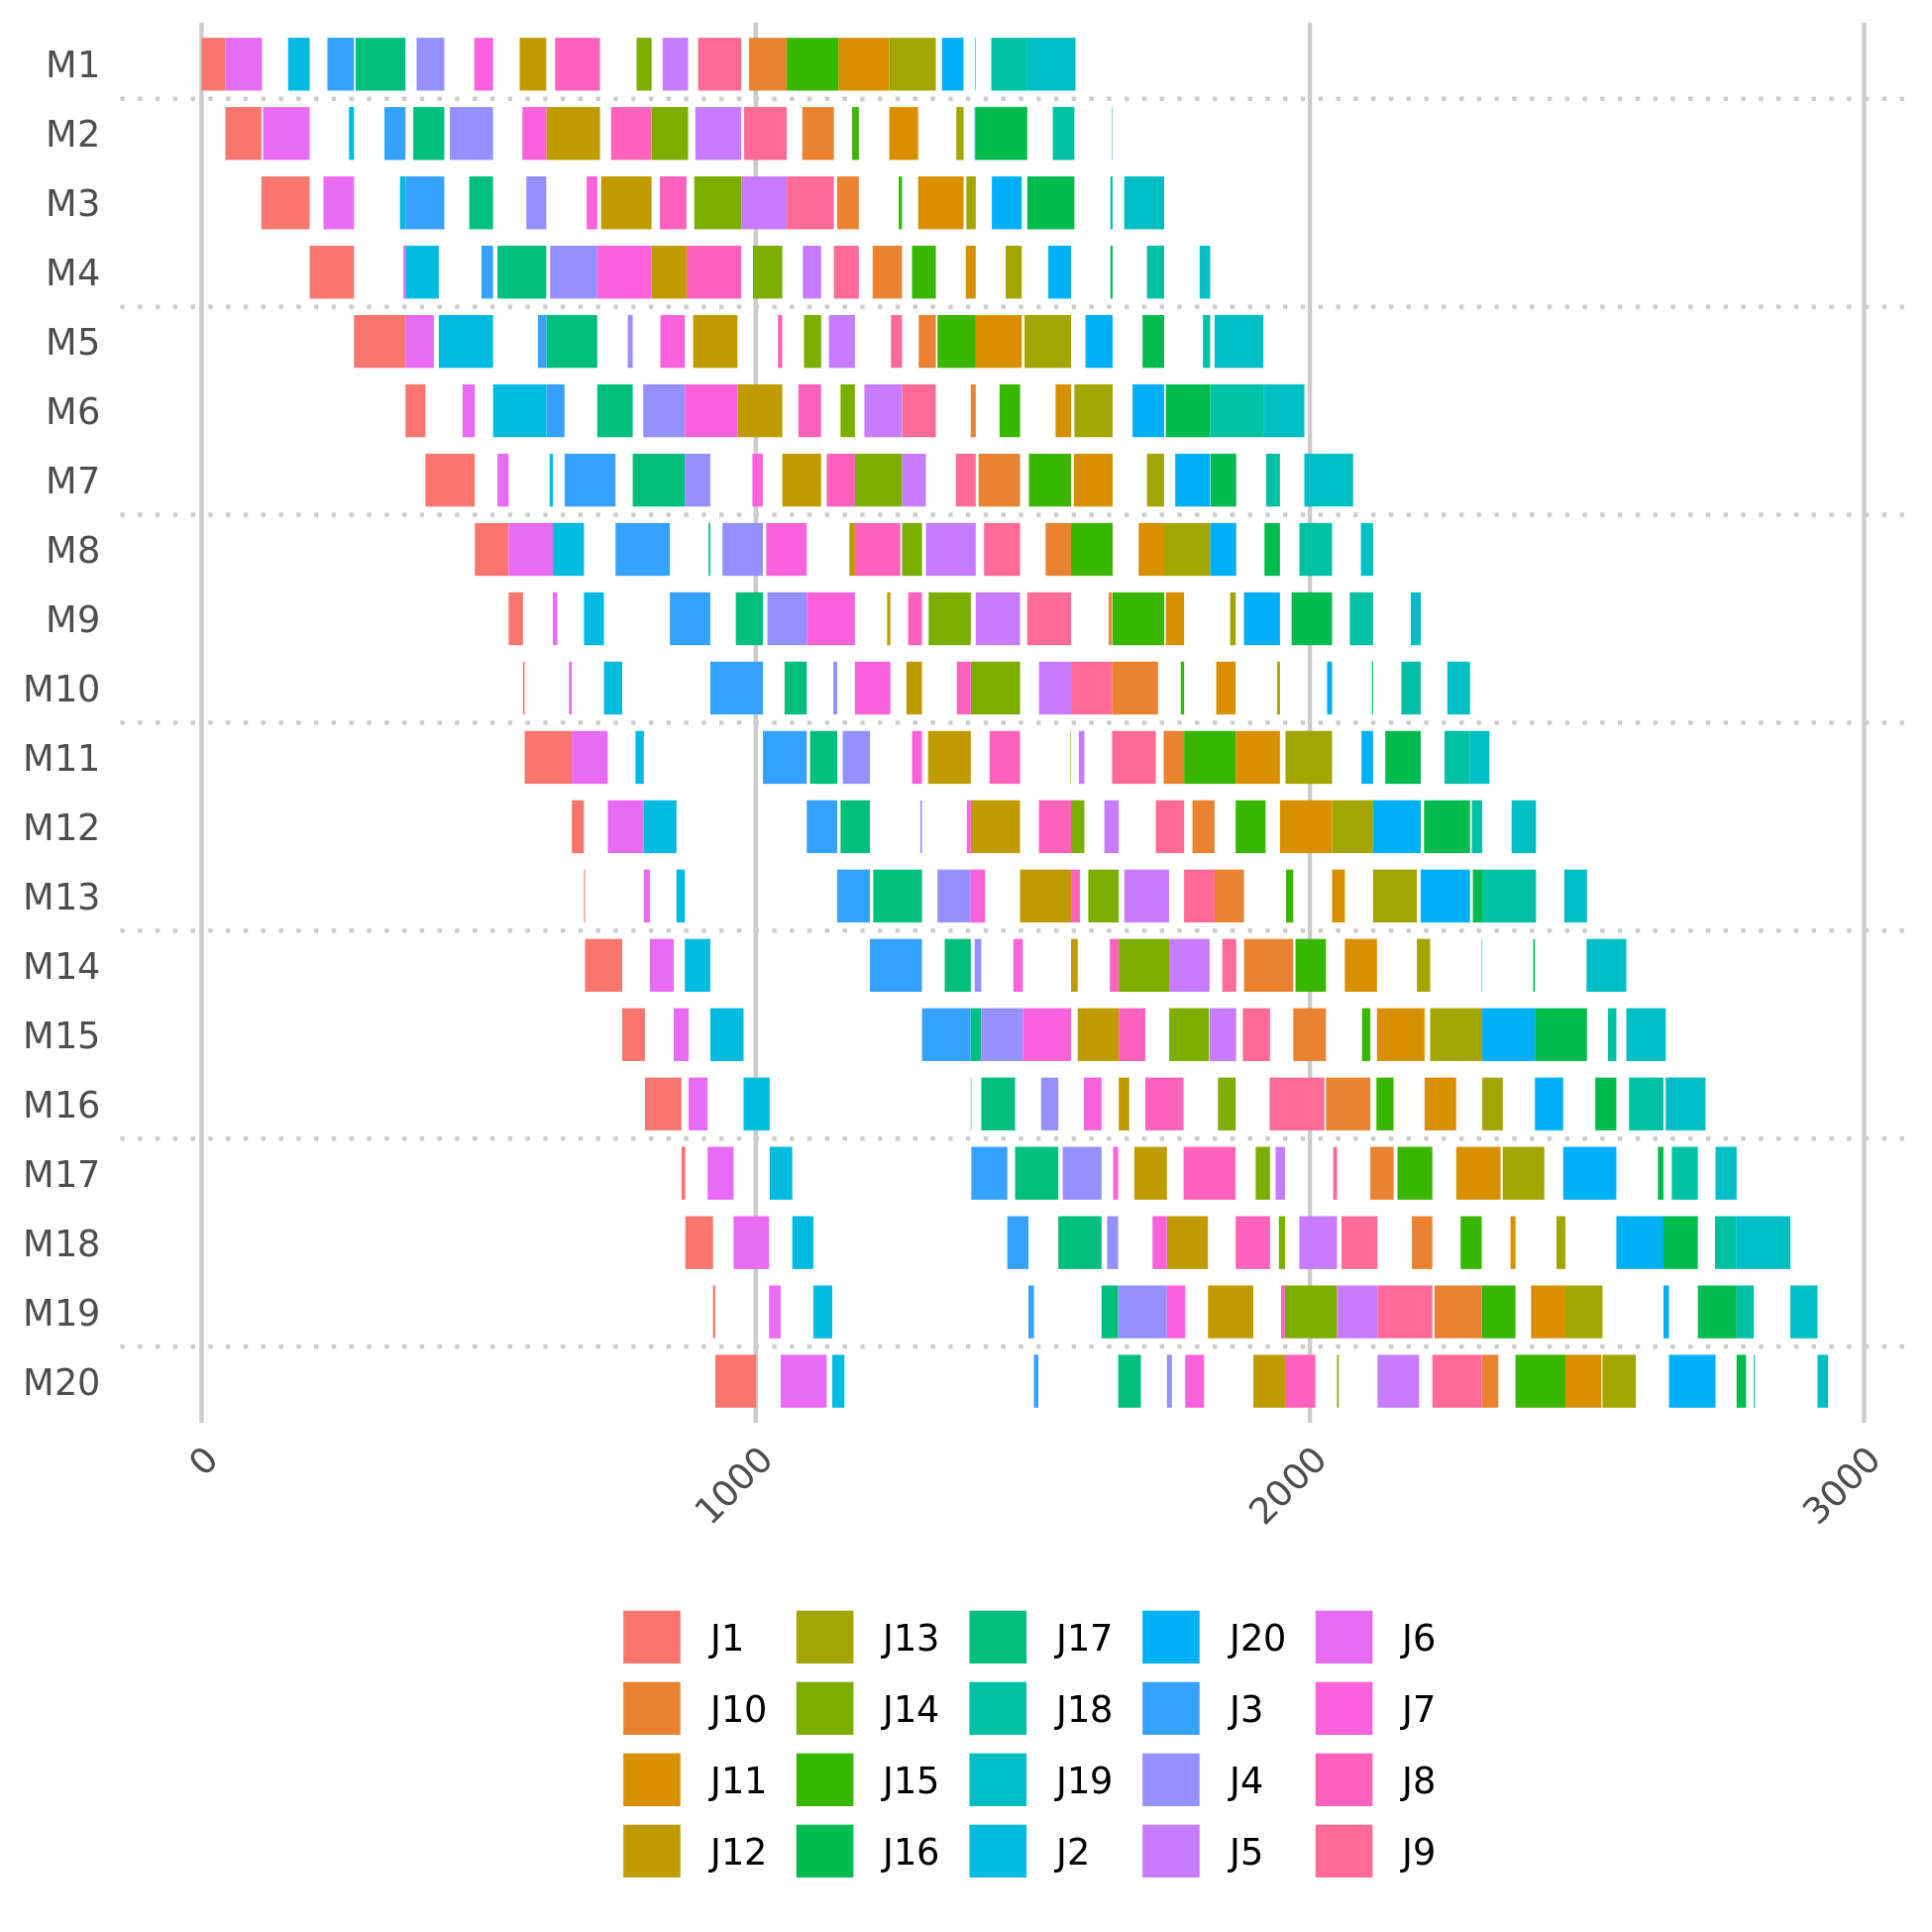
\includegraphics[width=\linewidth]{20_20_GC_2.png}
					\captionof{figure}{Gantt Chart for file 21.txt}
					
					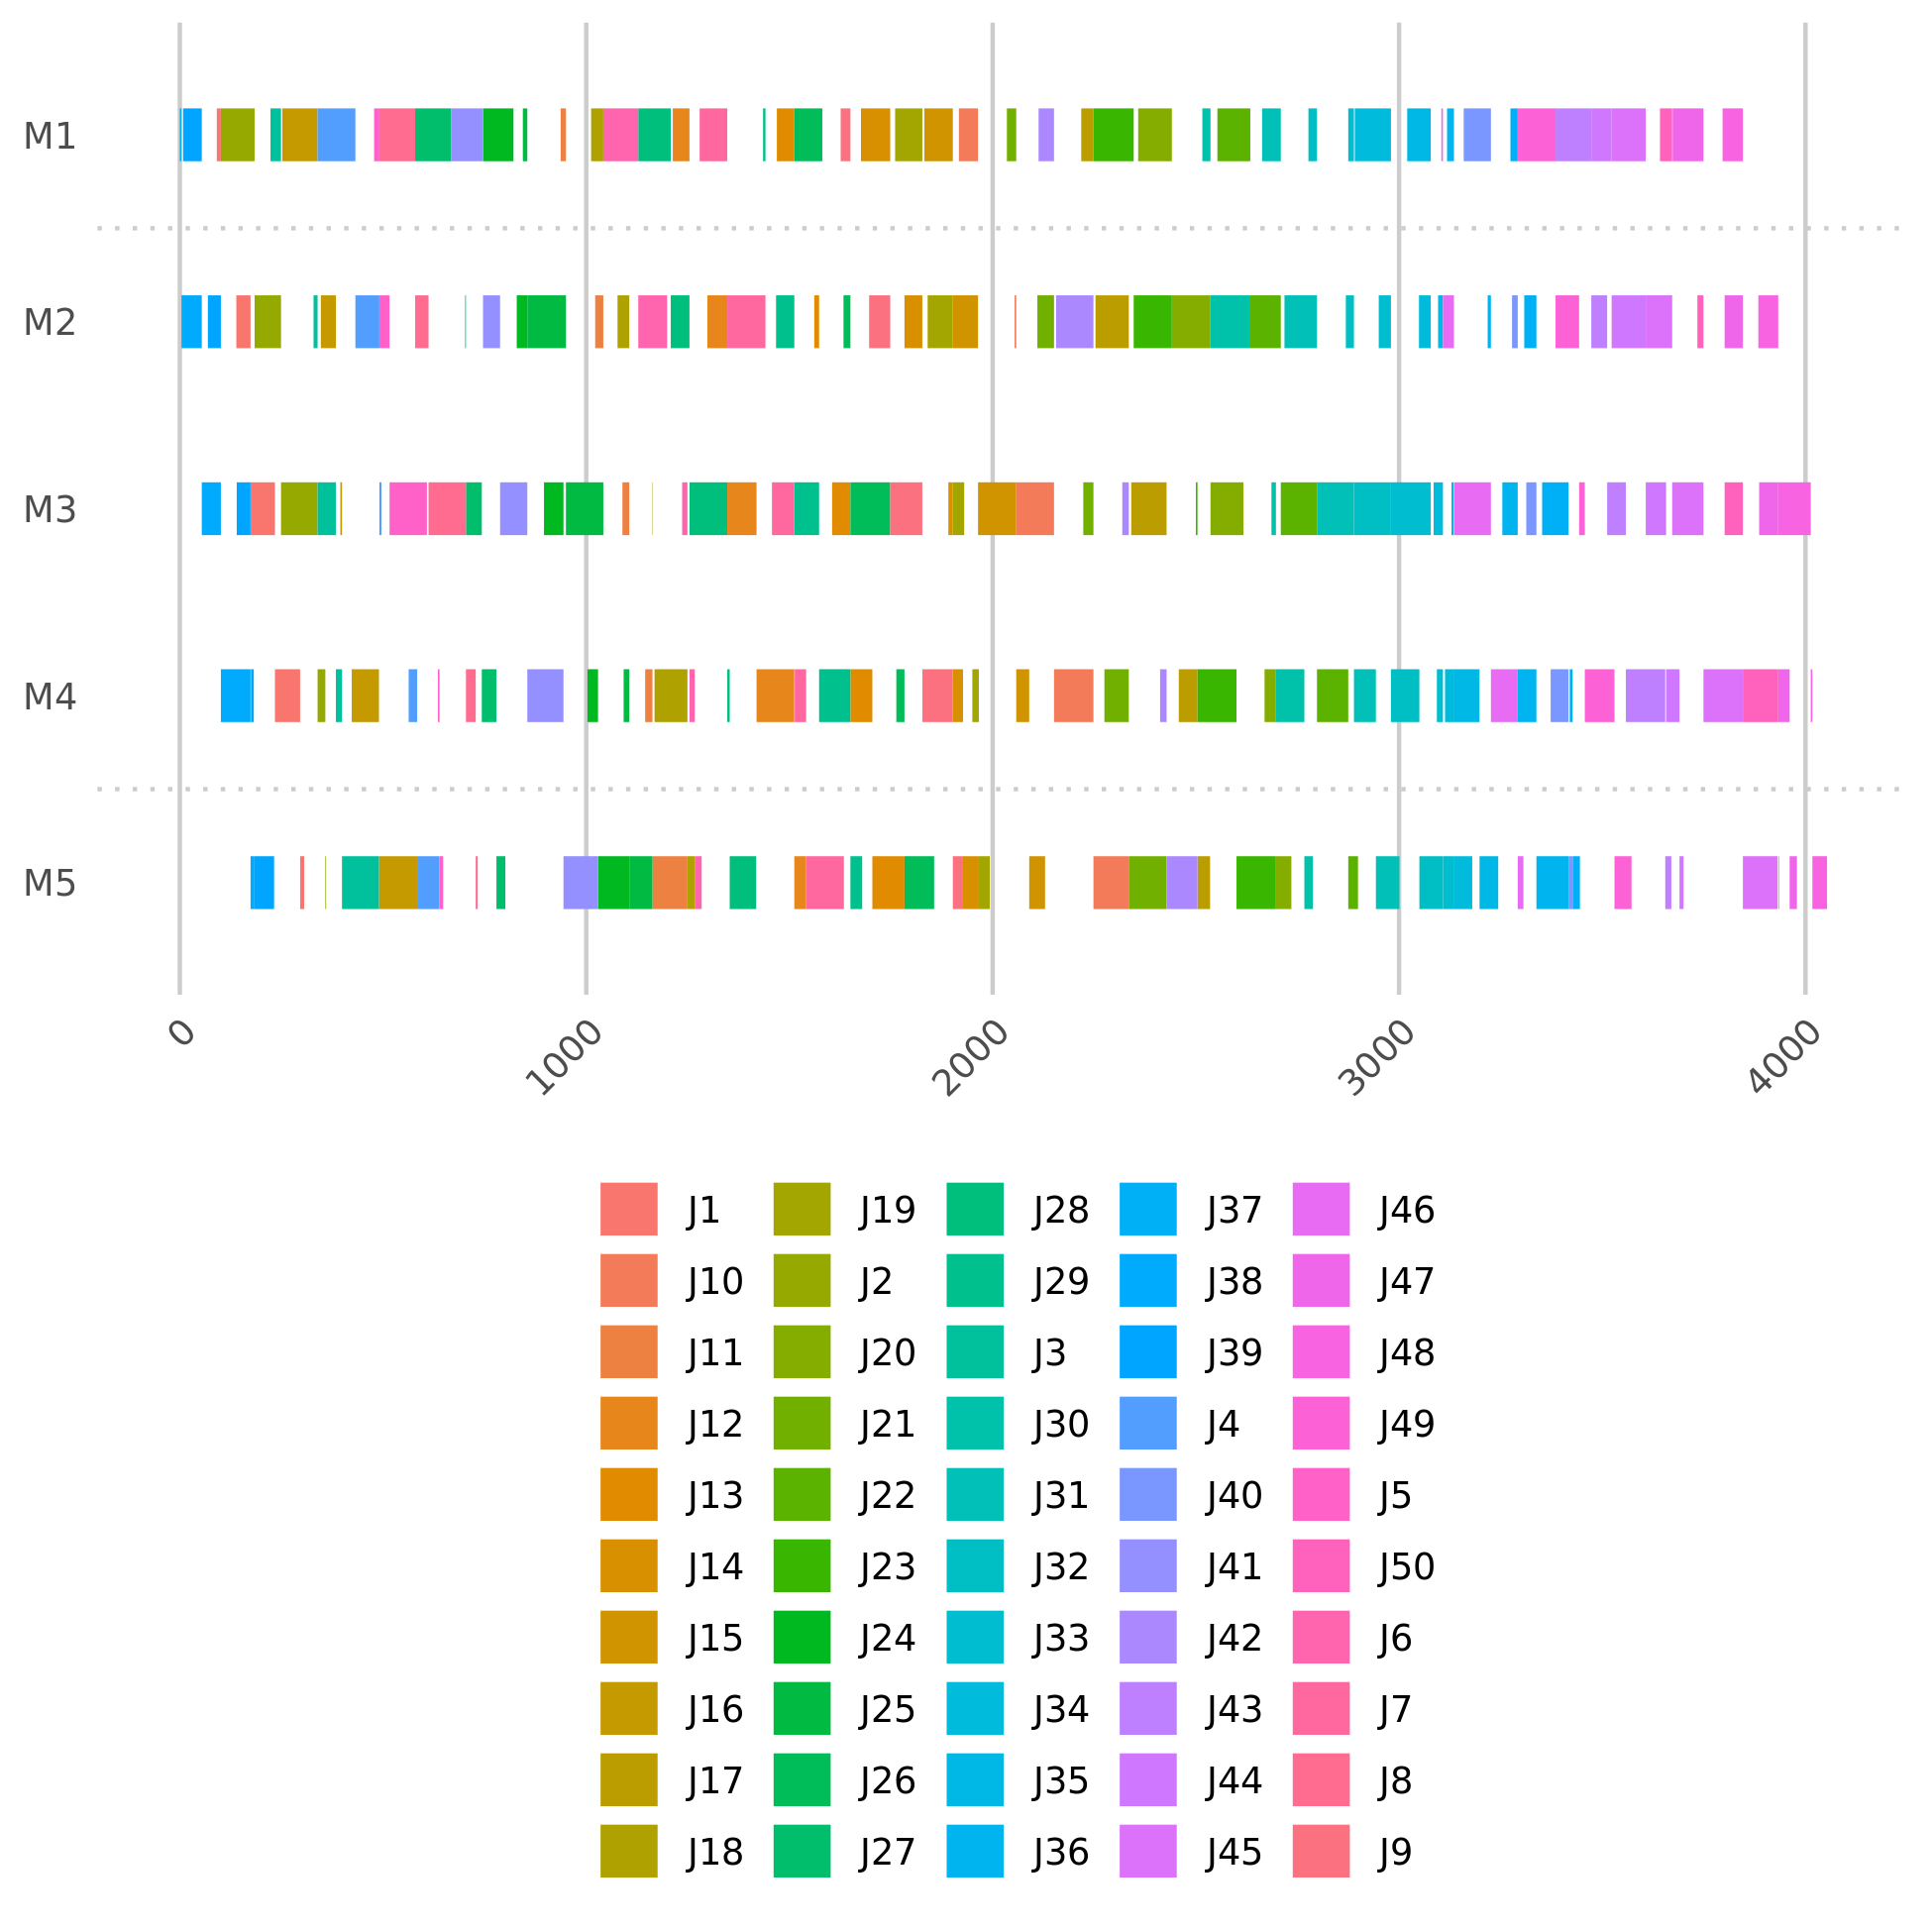
\includegraphics[width=\linewidth]{5_50_GC_2.png}
					\captionof{figure}{Gantt Chart for file 31.txt}
					
					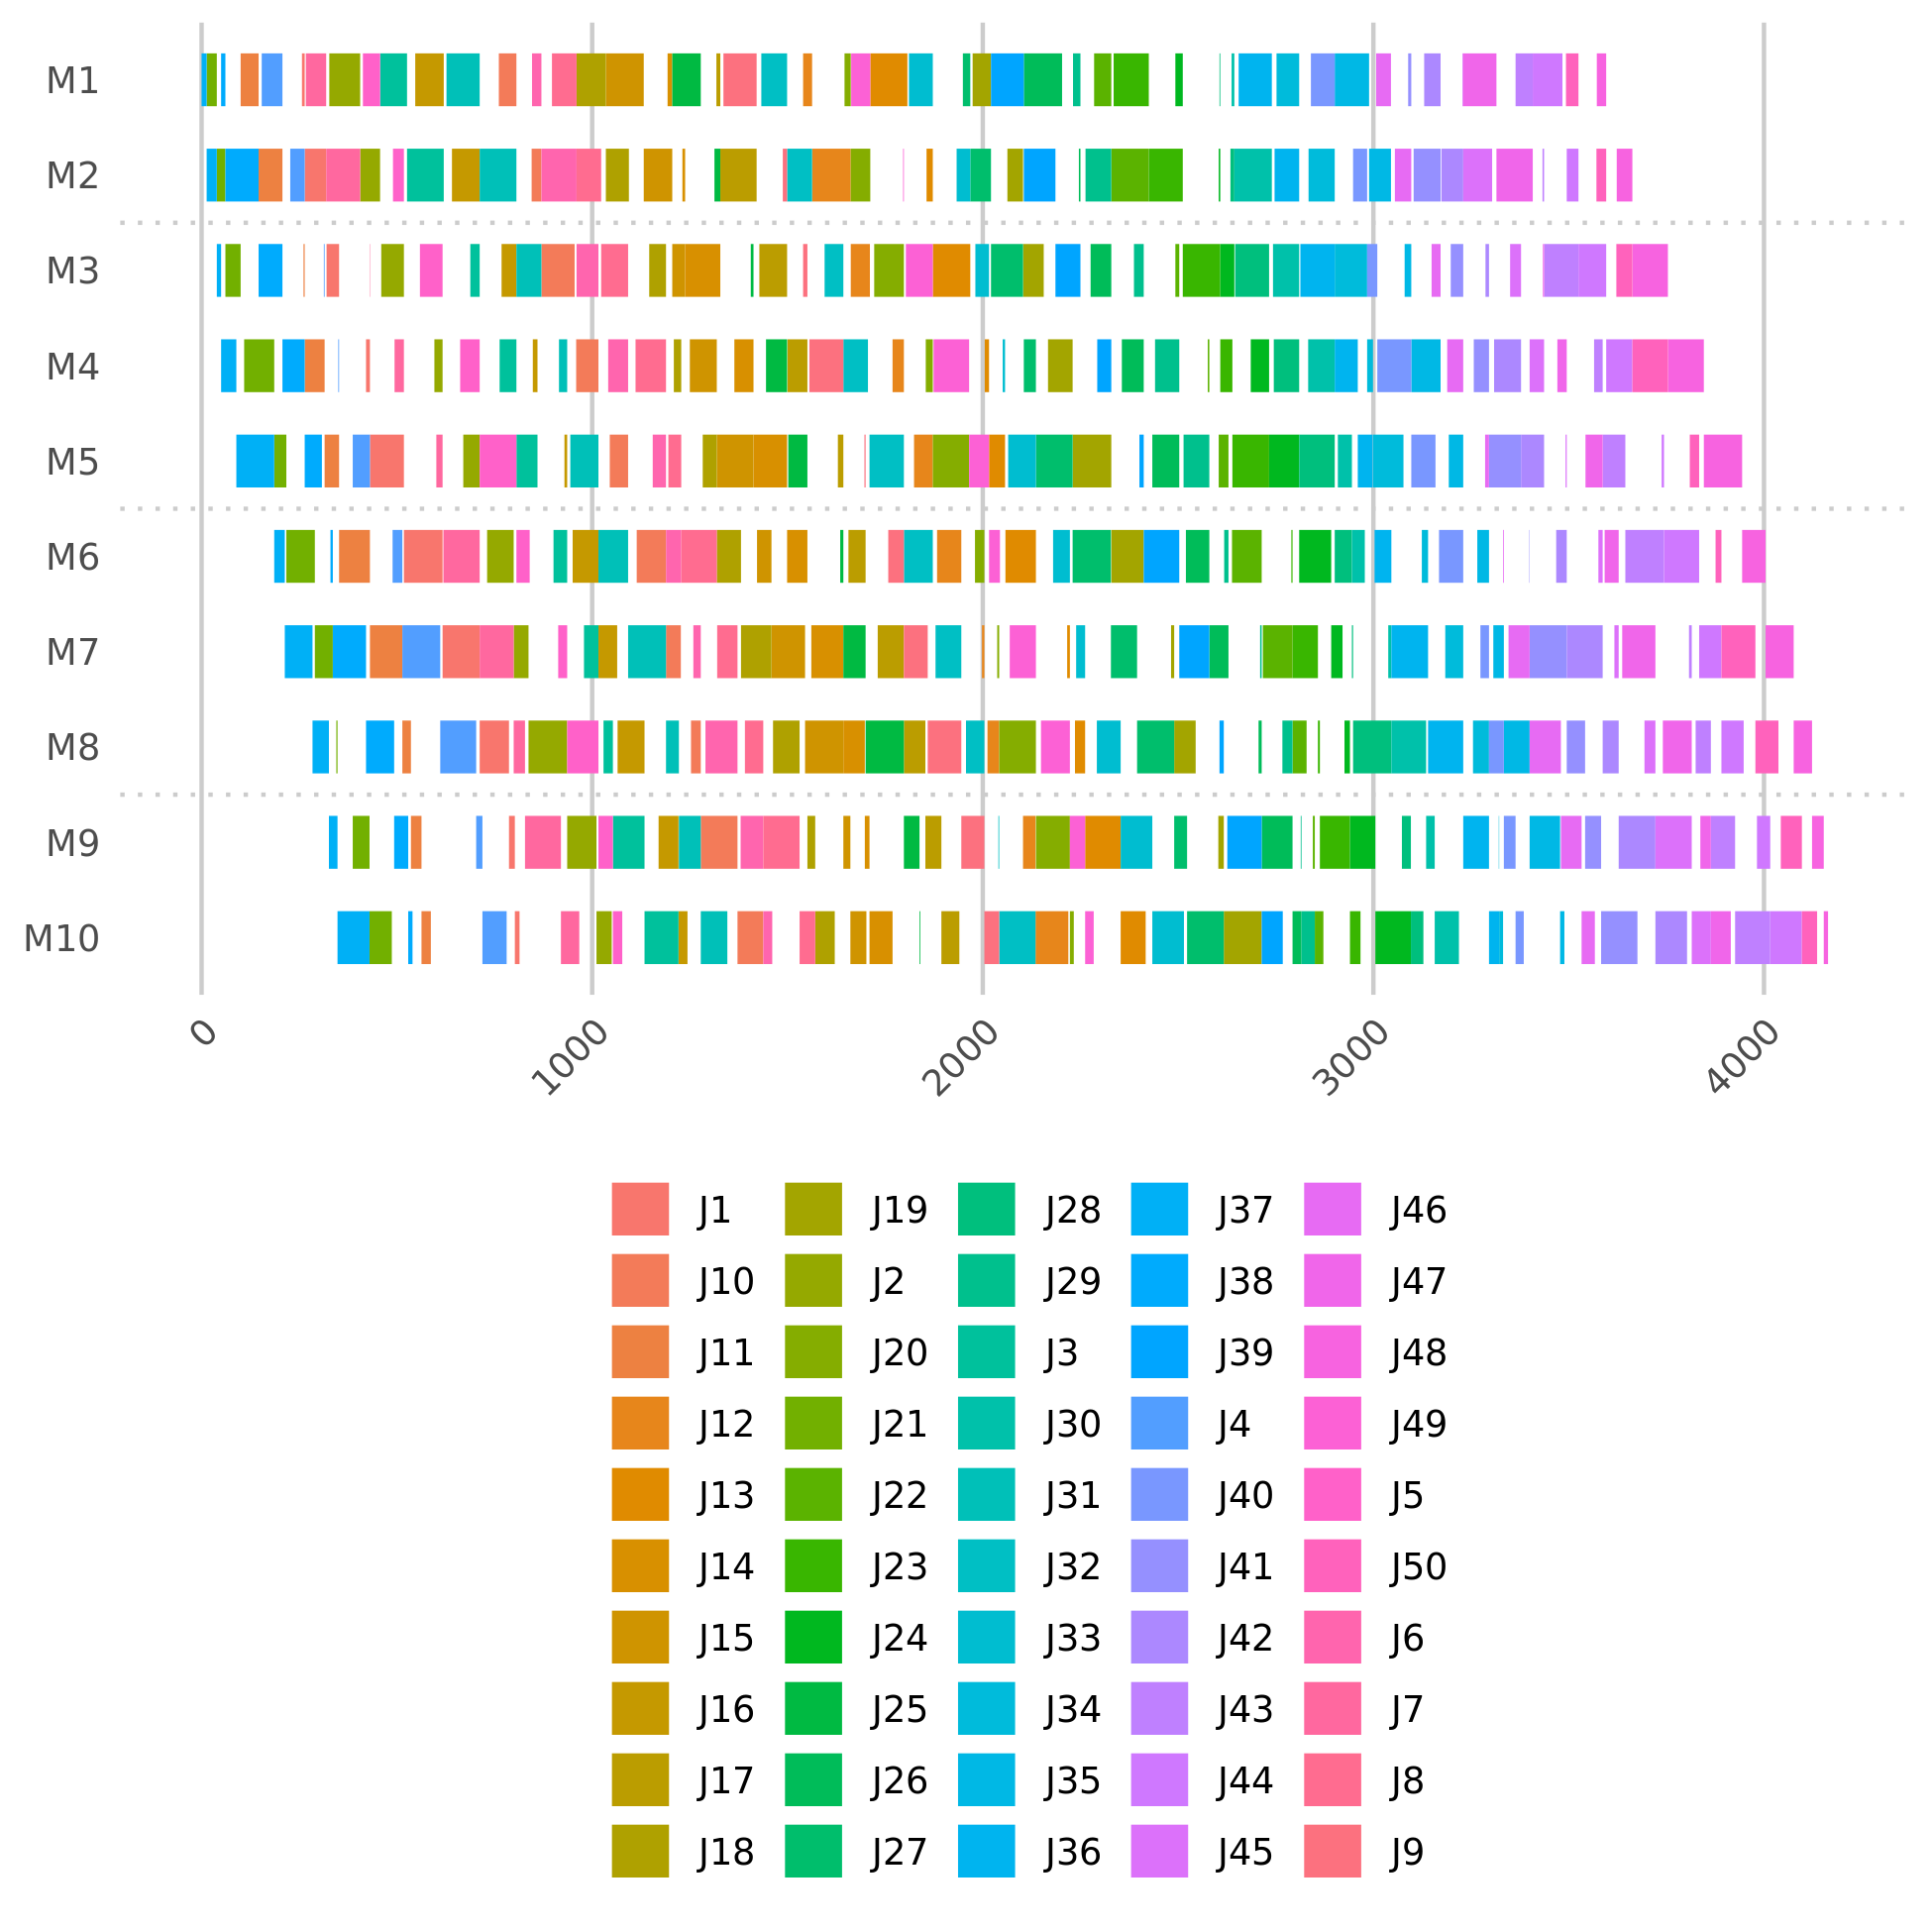
\includegraphics[width=\linewidth]{10_50_GC_2.png}
					\captionof{figure}{Gantt Chart for file 41.txt}
					
					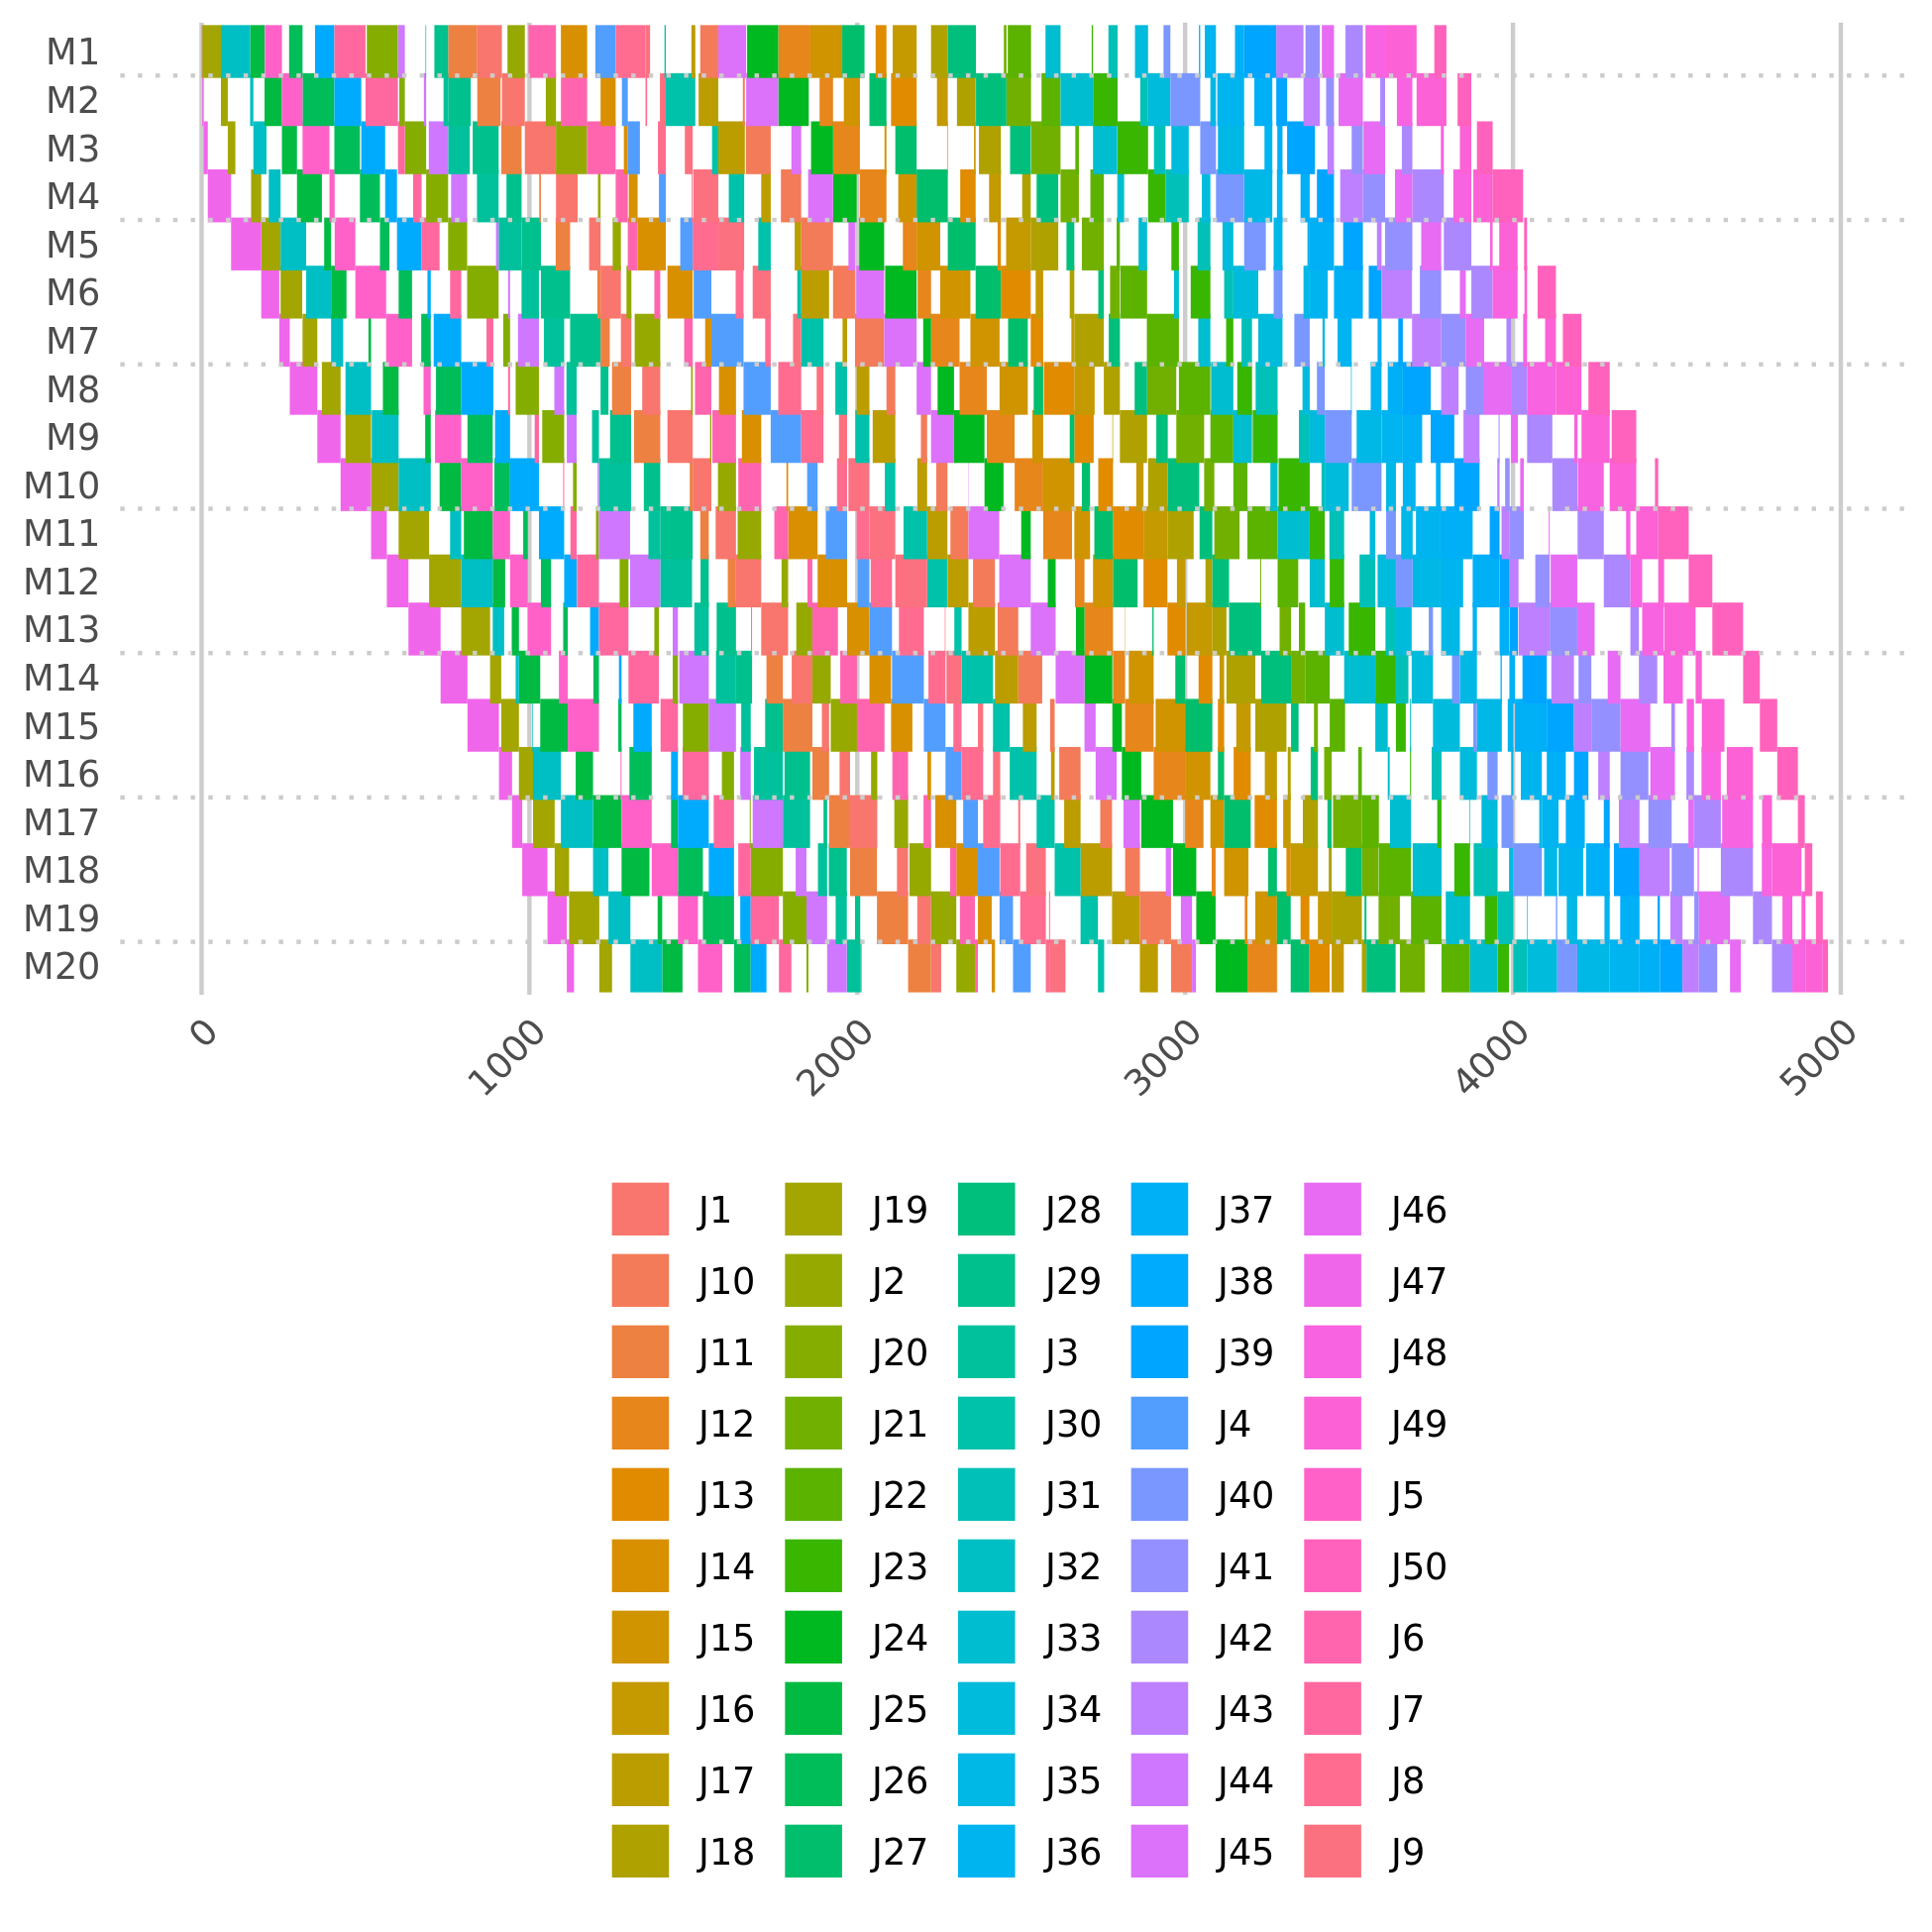
\includegraphics[width=\linewidth]{20_50_GC_2.png}
					\captionof{figure}{Gantt Chart for file 51.txt}
					
					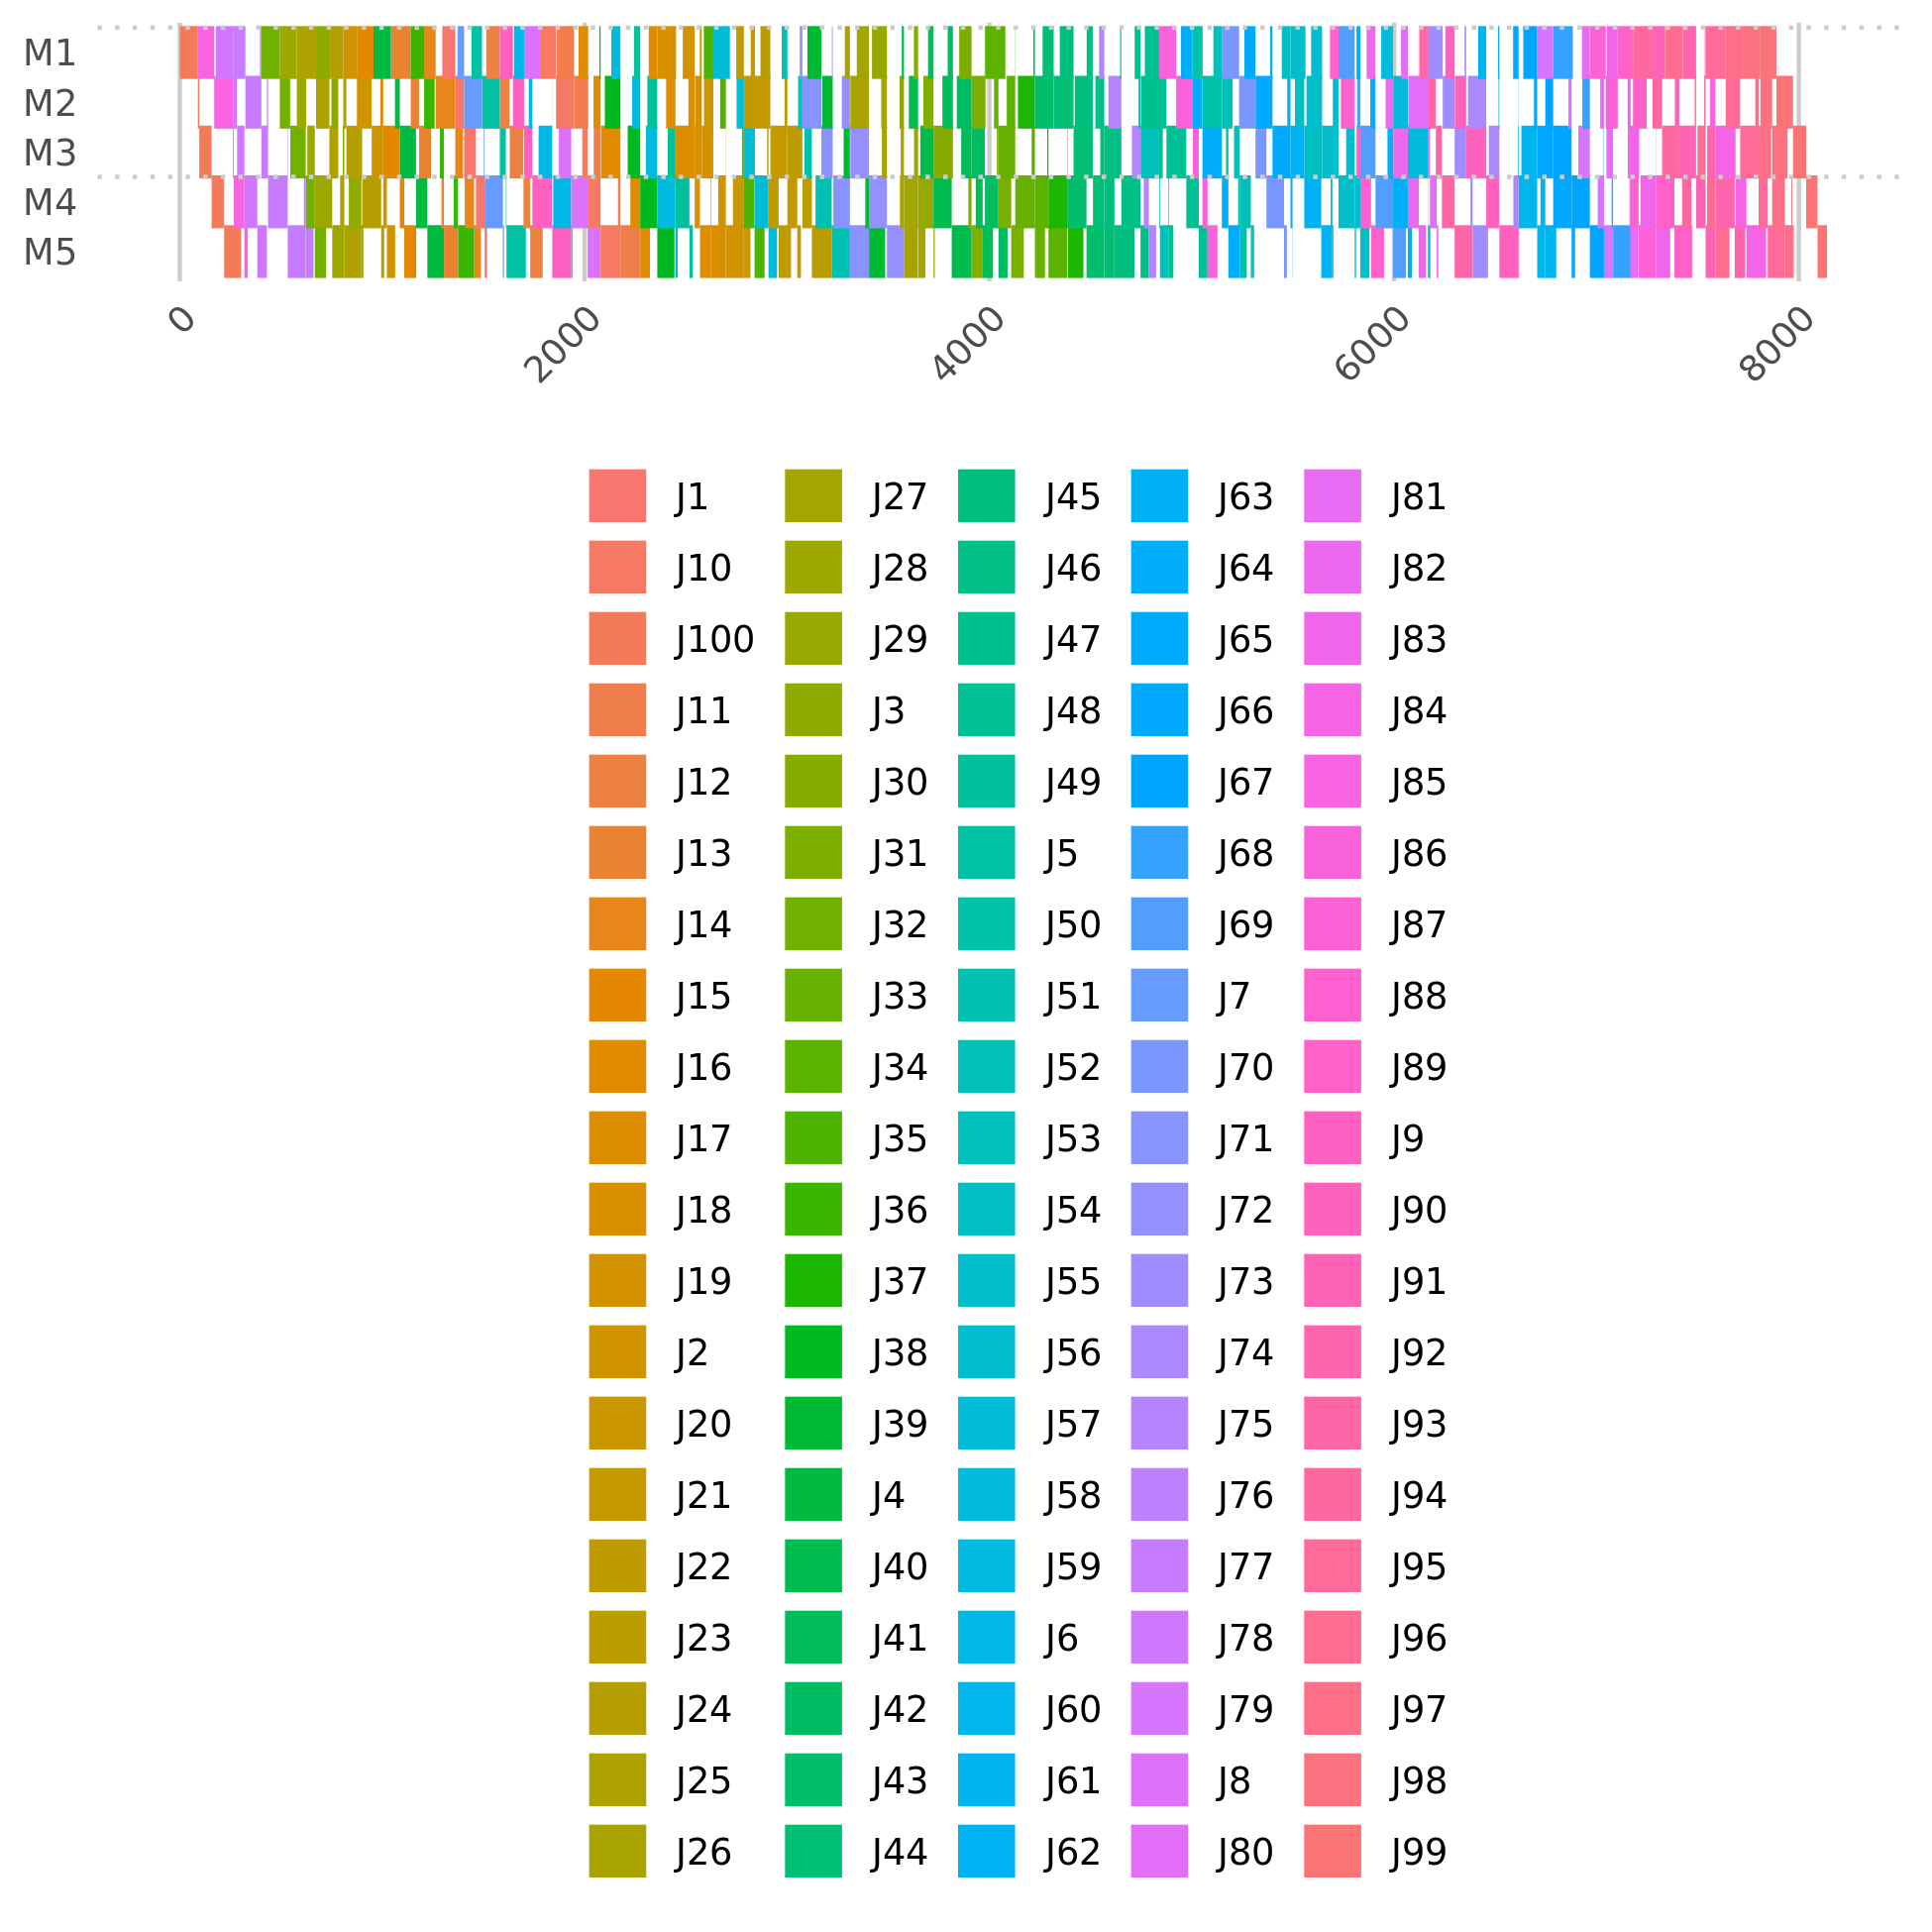
\includegraphics[width=\linewidth]{5_100_GC_2.png}
					\captionof{figure}{Gantt Chart for file 61.txt}
					
					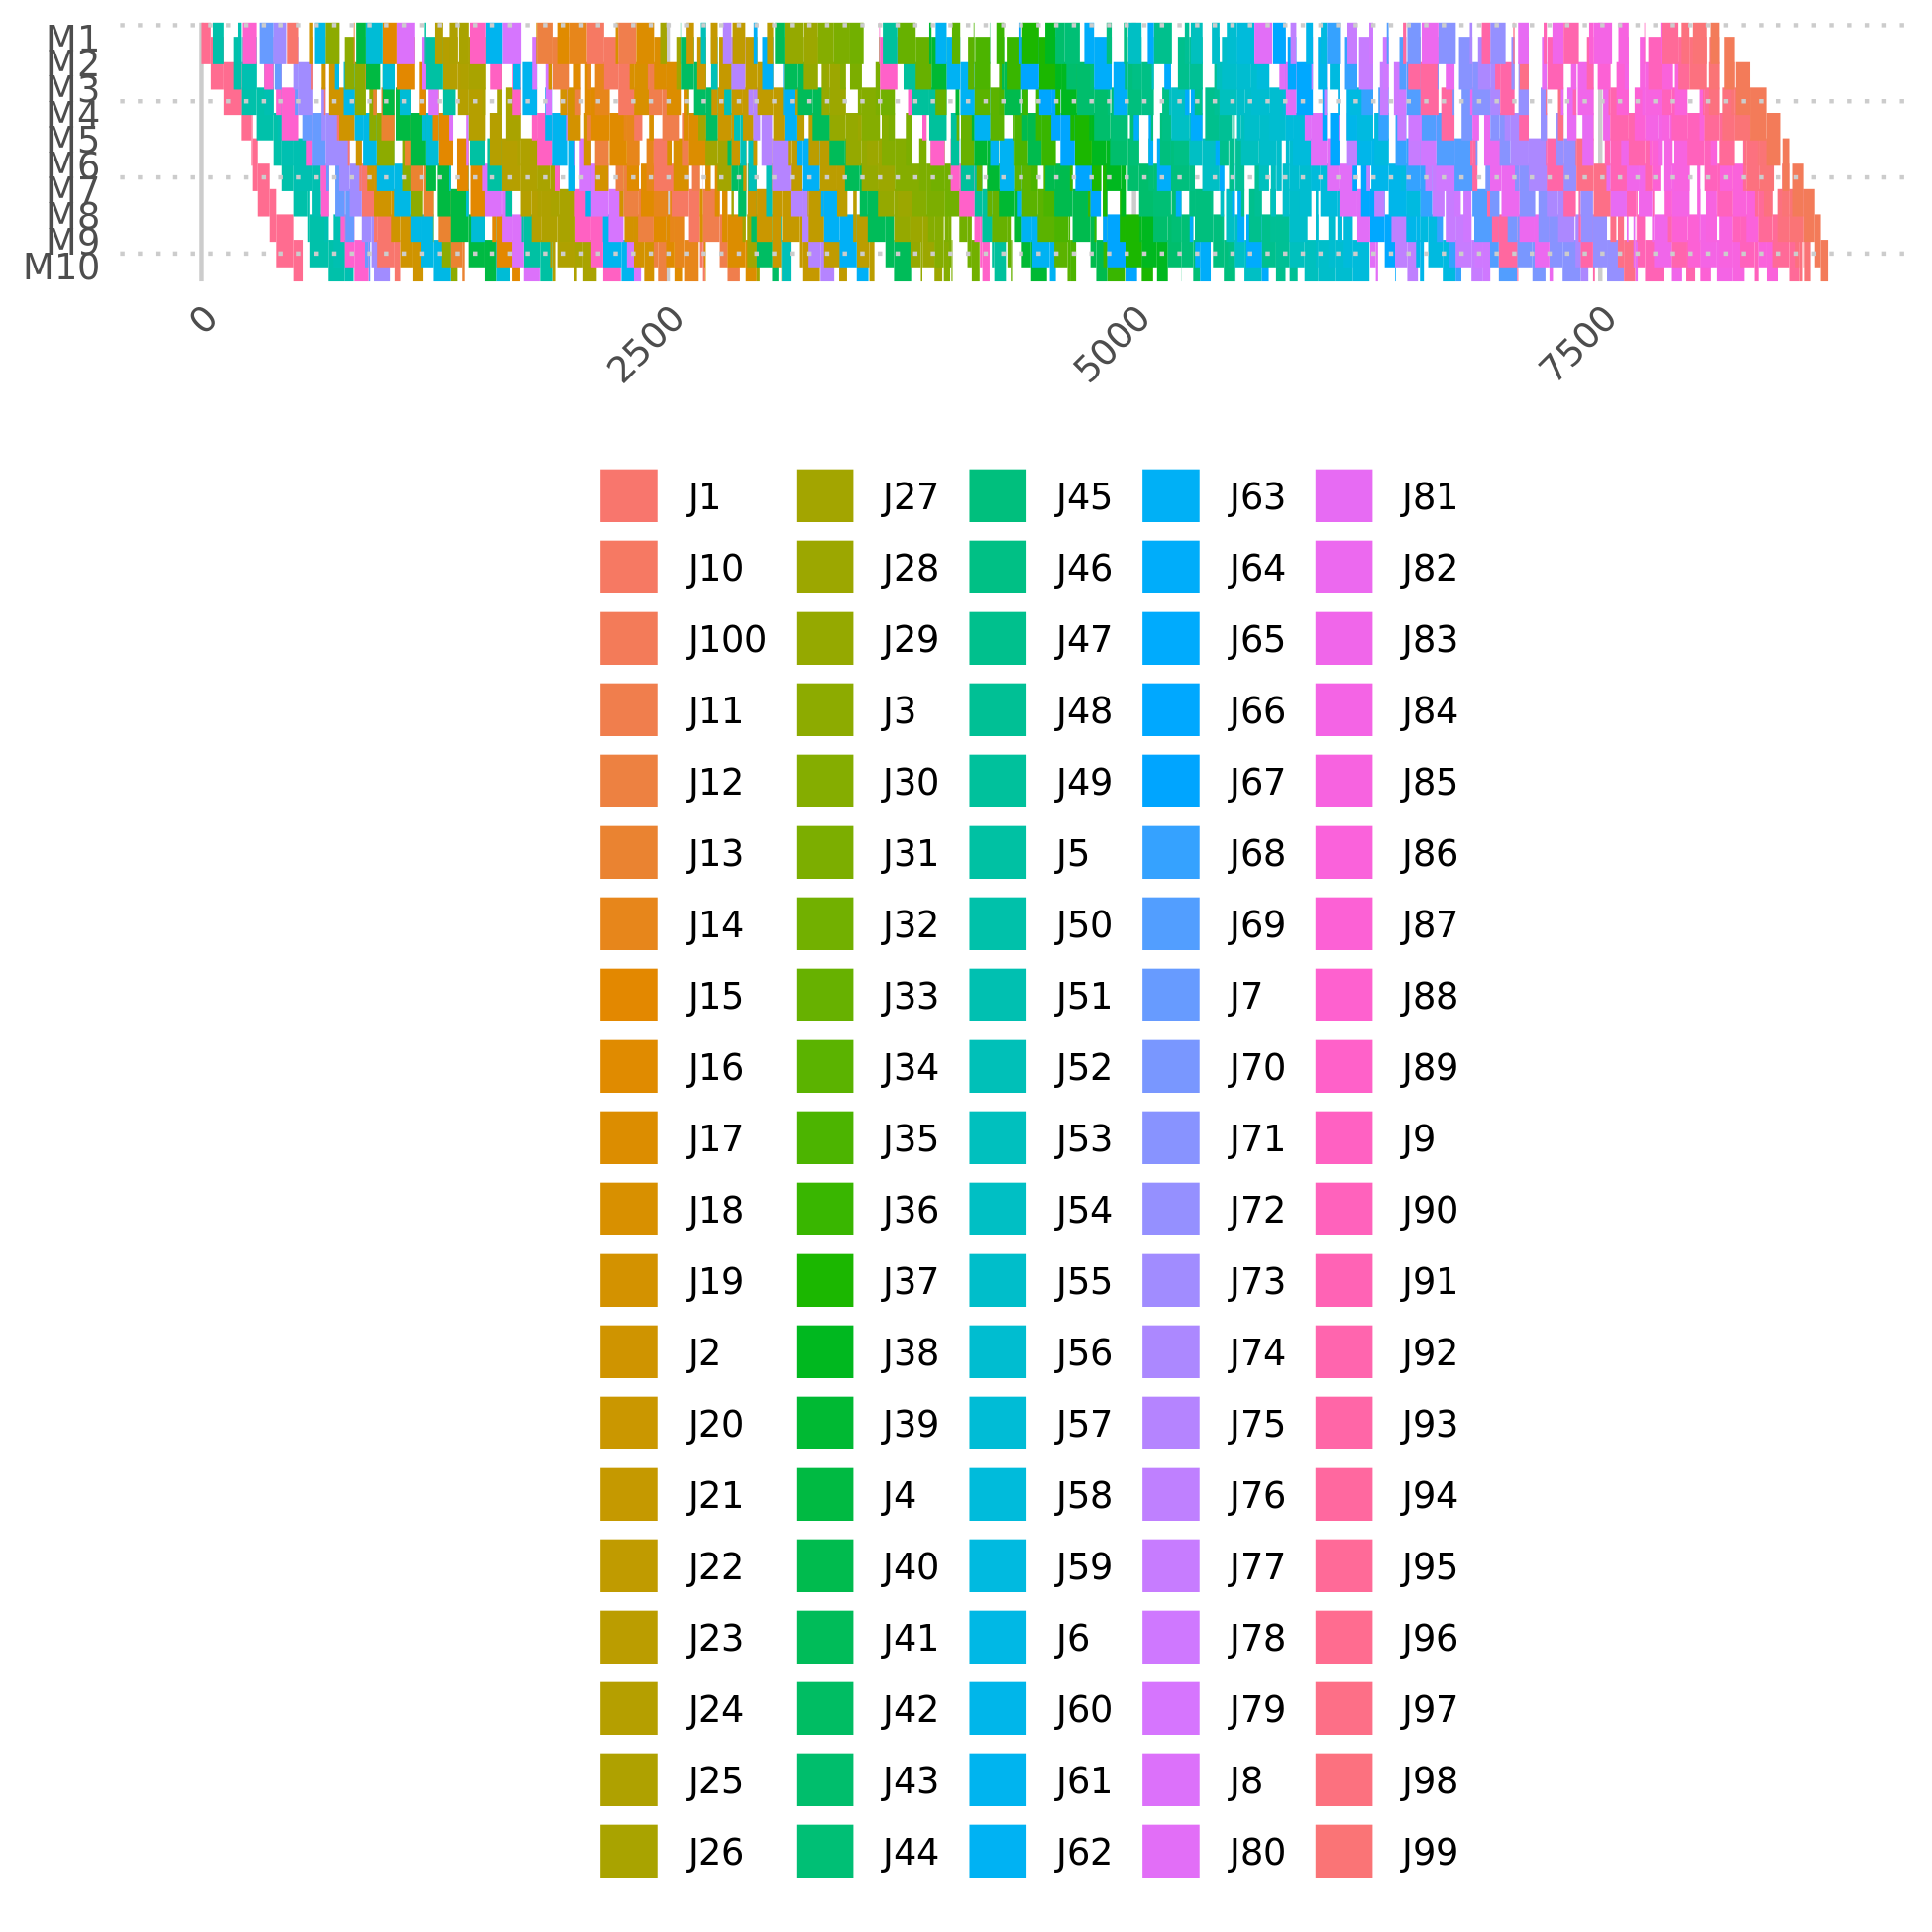
\includegraphics[width=\linewidth]{10_100_GC_2.png}
					\captionof{figure}{Gantt Chart for file 71.txt}
					
					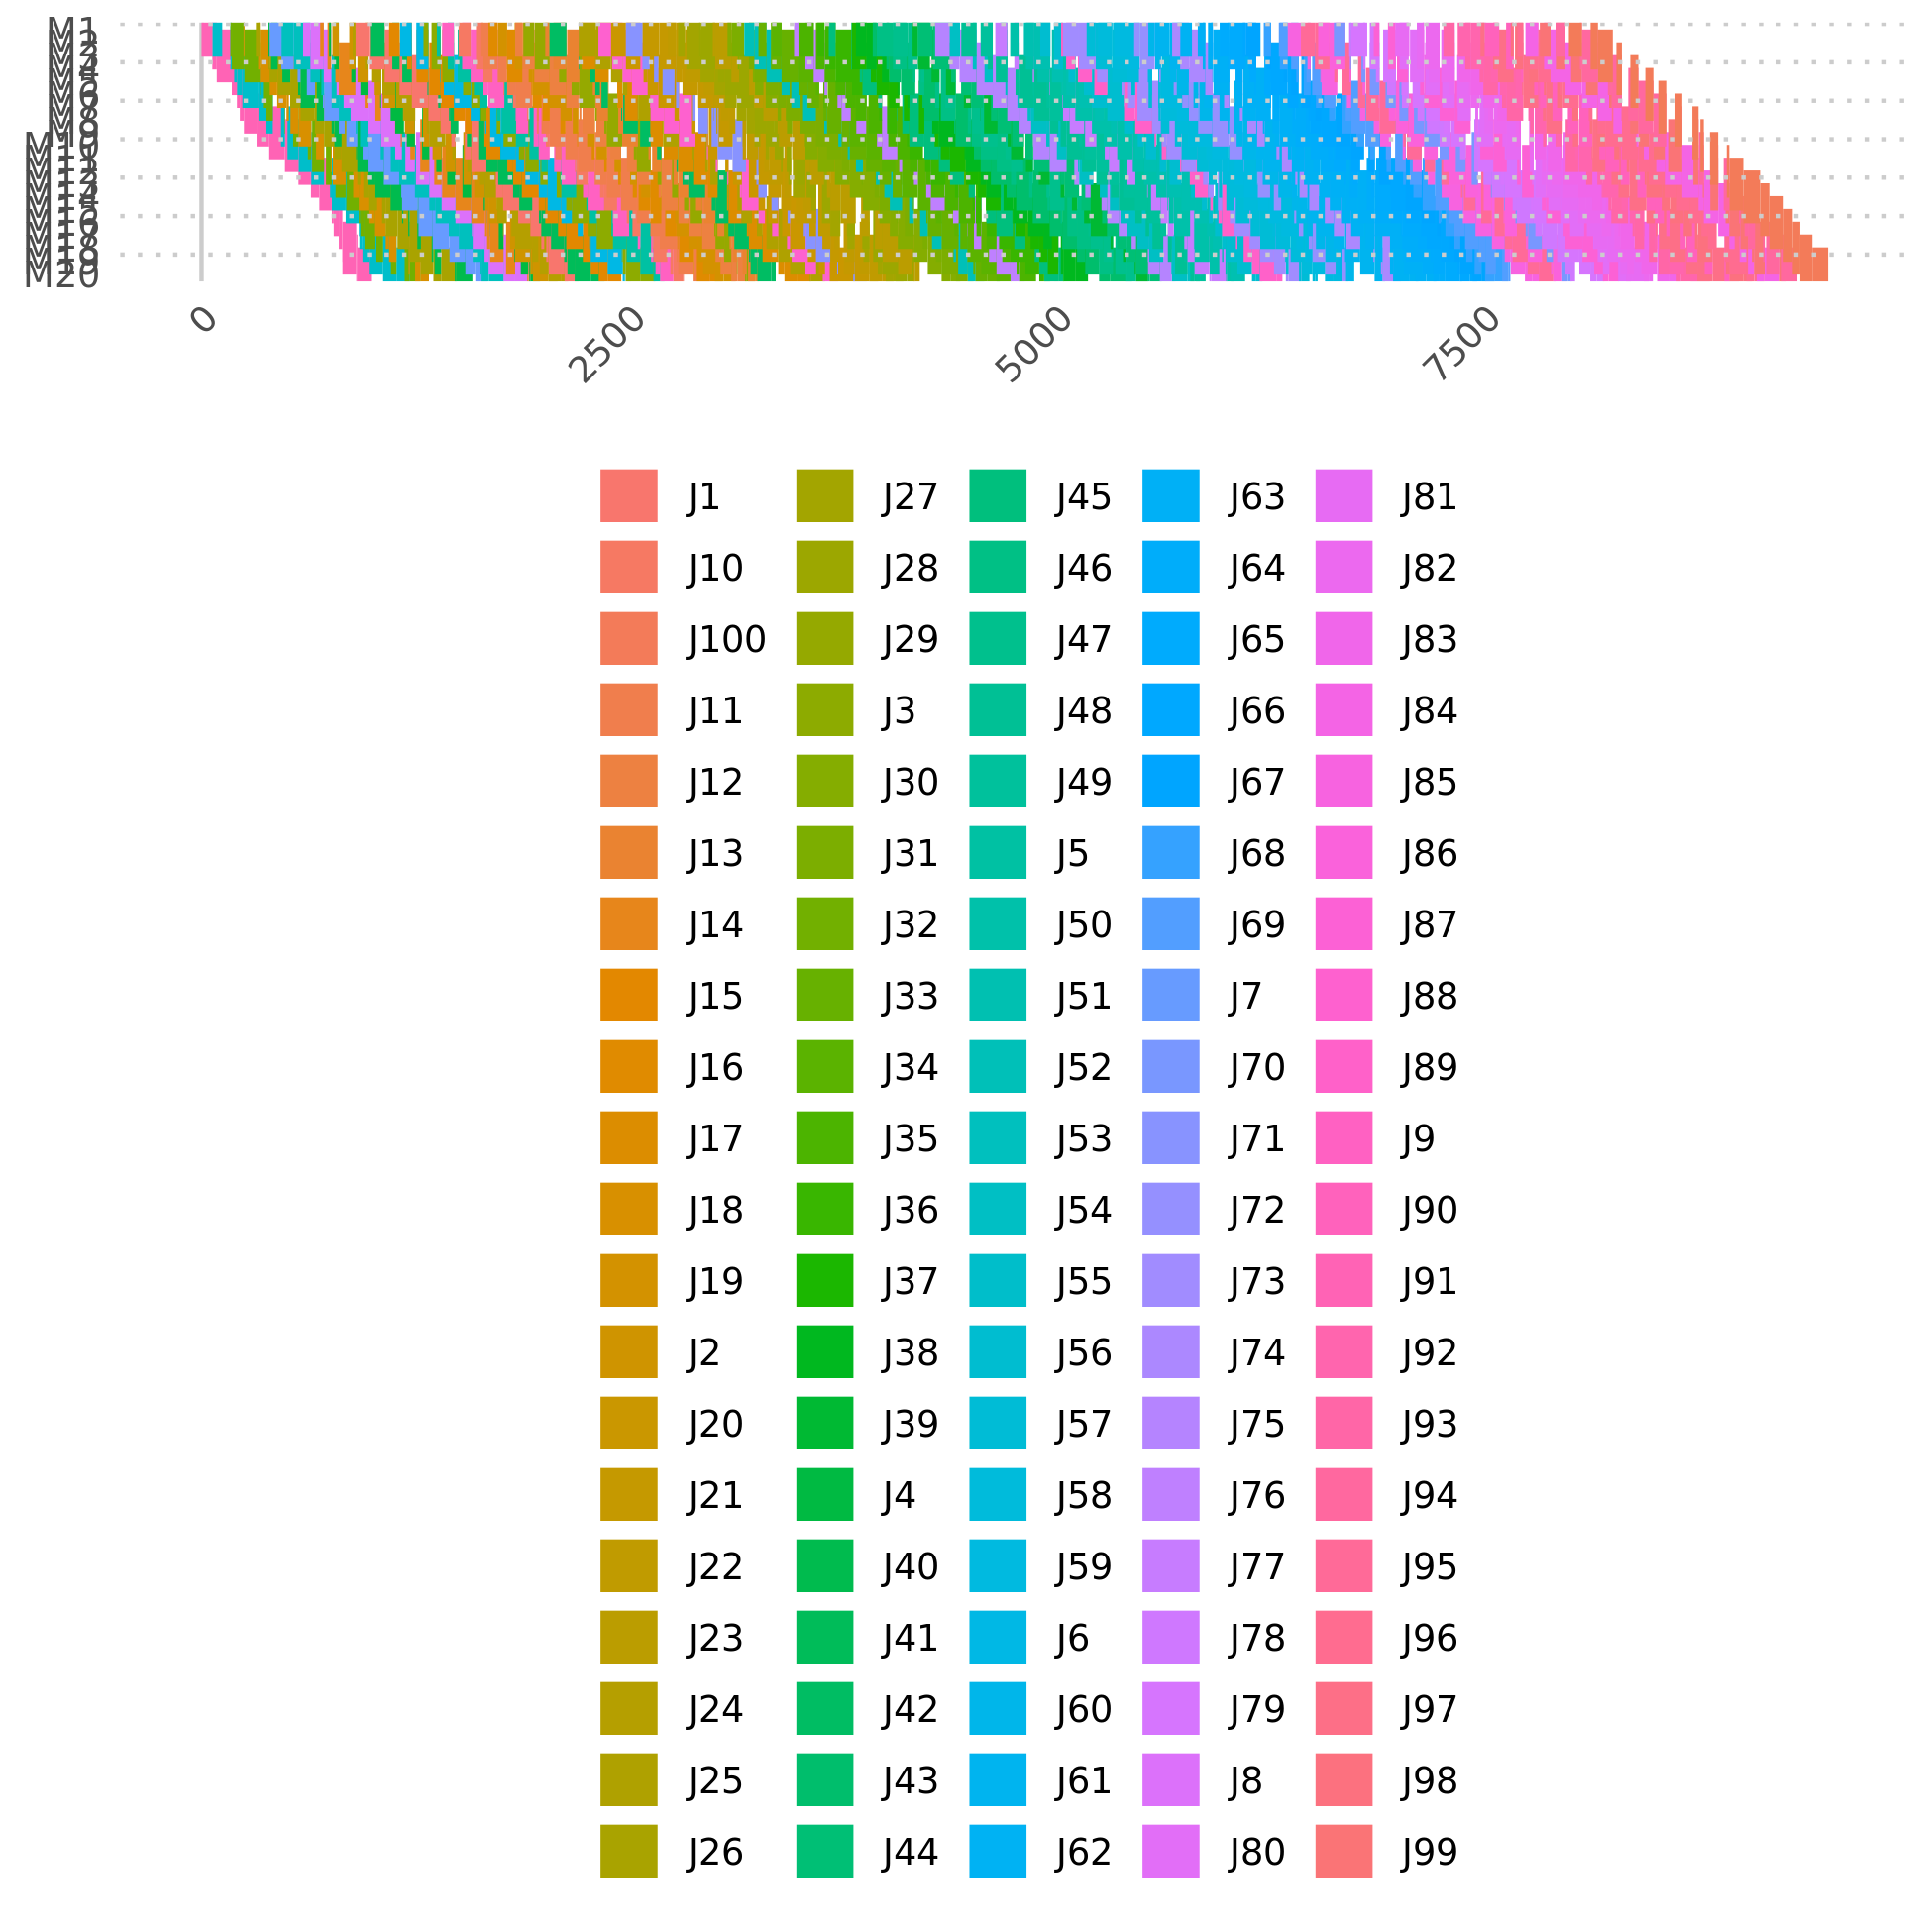
\includegraphics[width=\linewidth]{20_100_GC_2.png}
					\captionof{figure}{Gantt Chart for file 81.txt}
					
					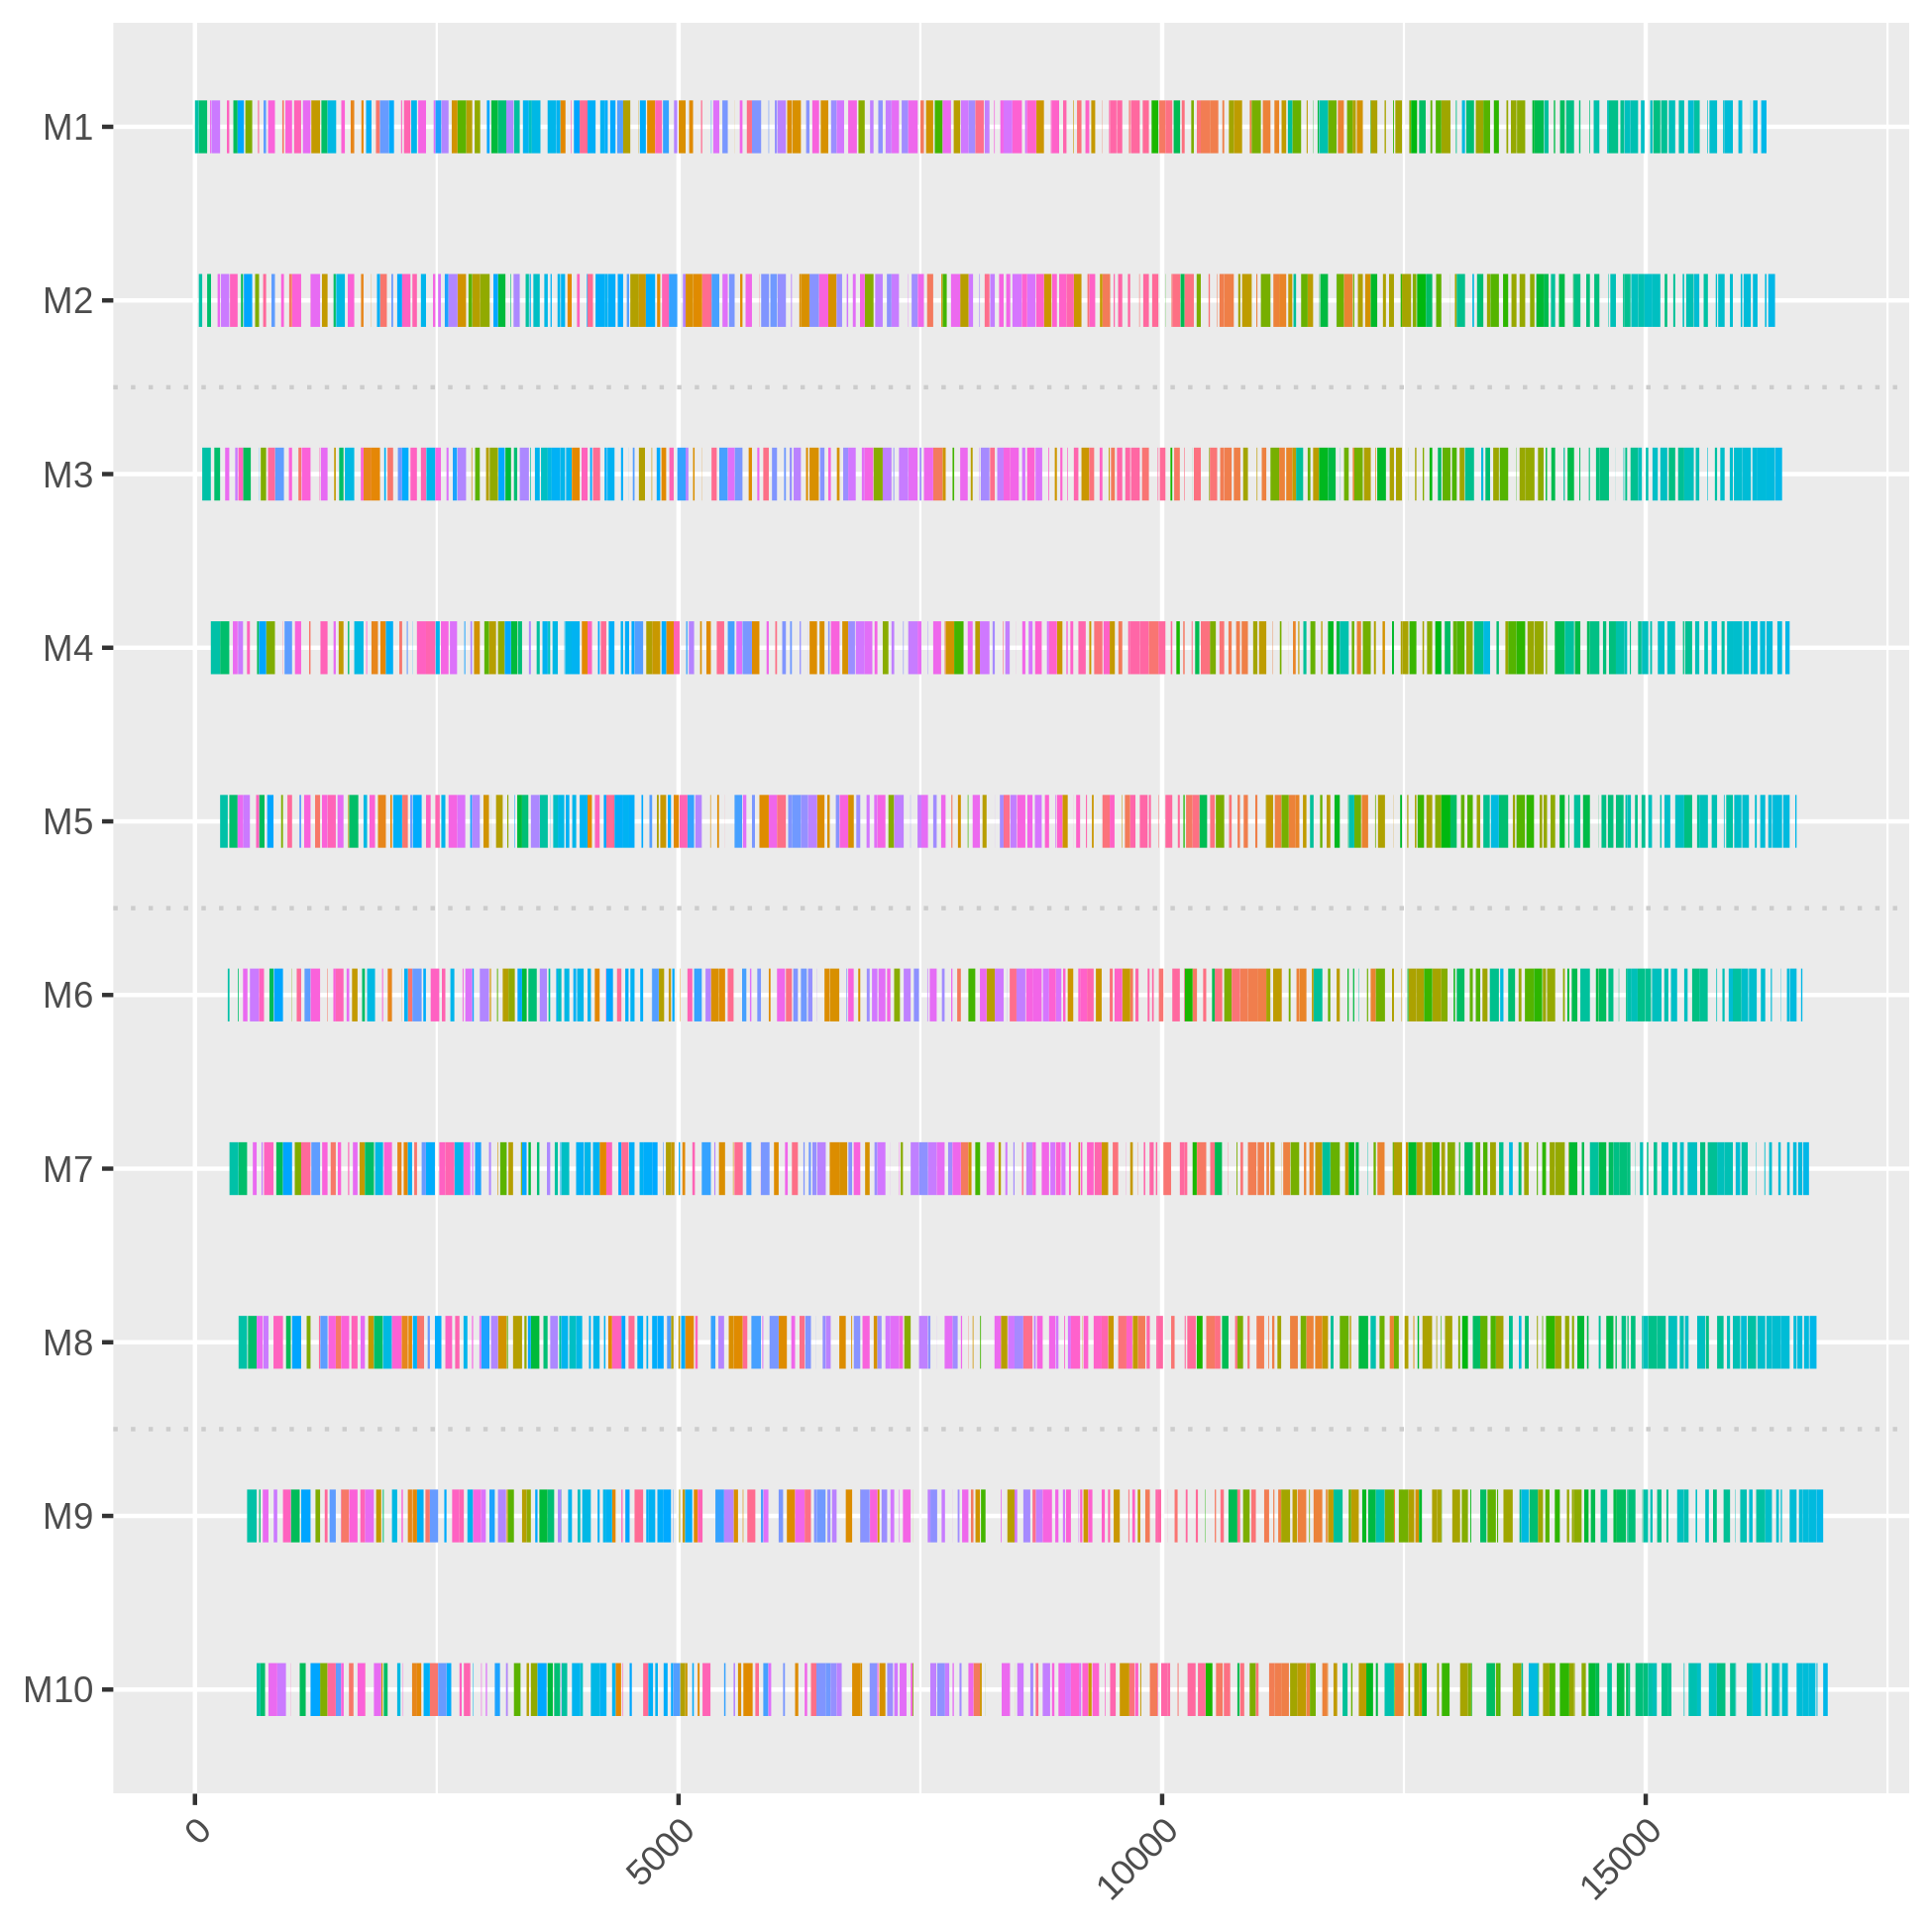
\includegraphics[width=\linewidth]{10_200_GC_2.png}
					\captionof{figure}{Gantt Chart for file 91.txt}
					
					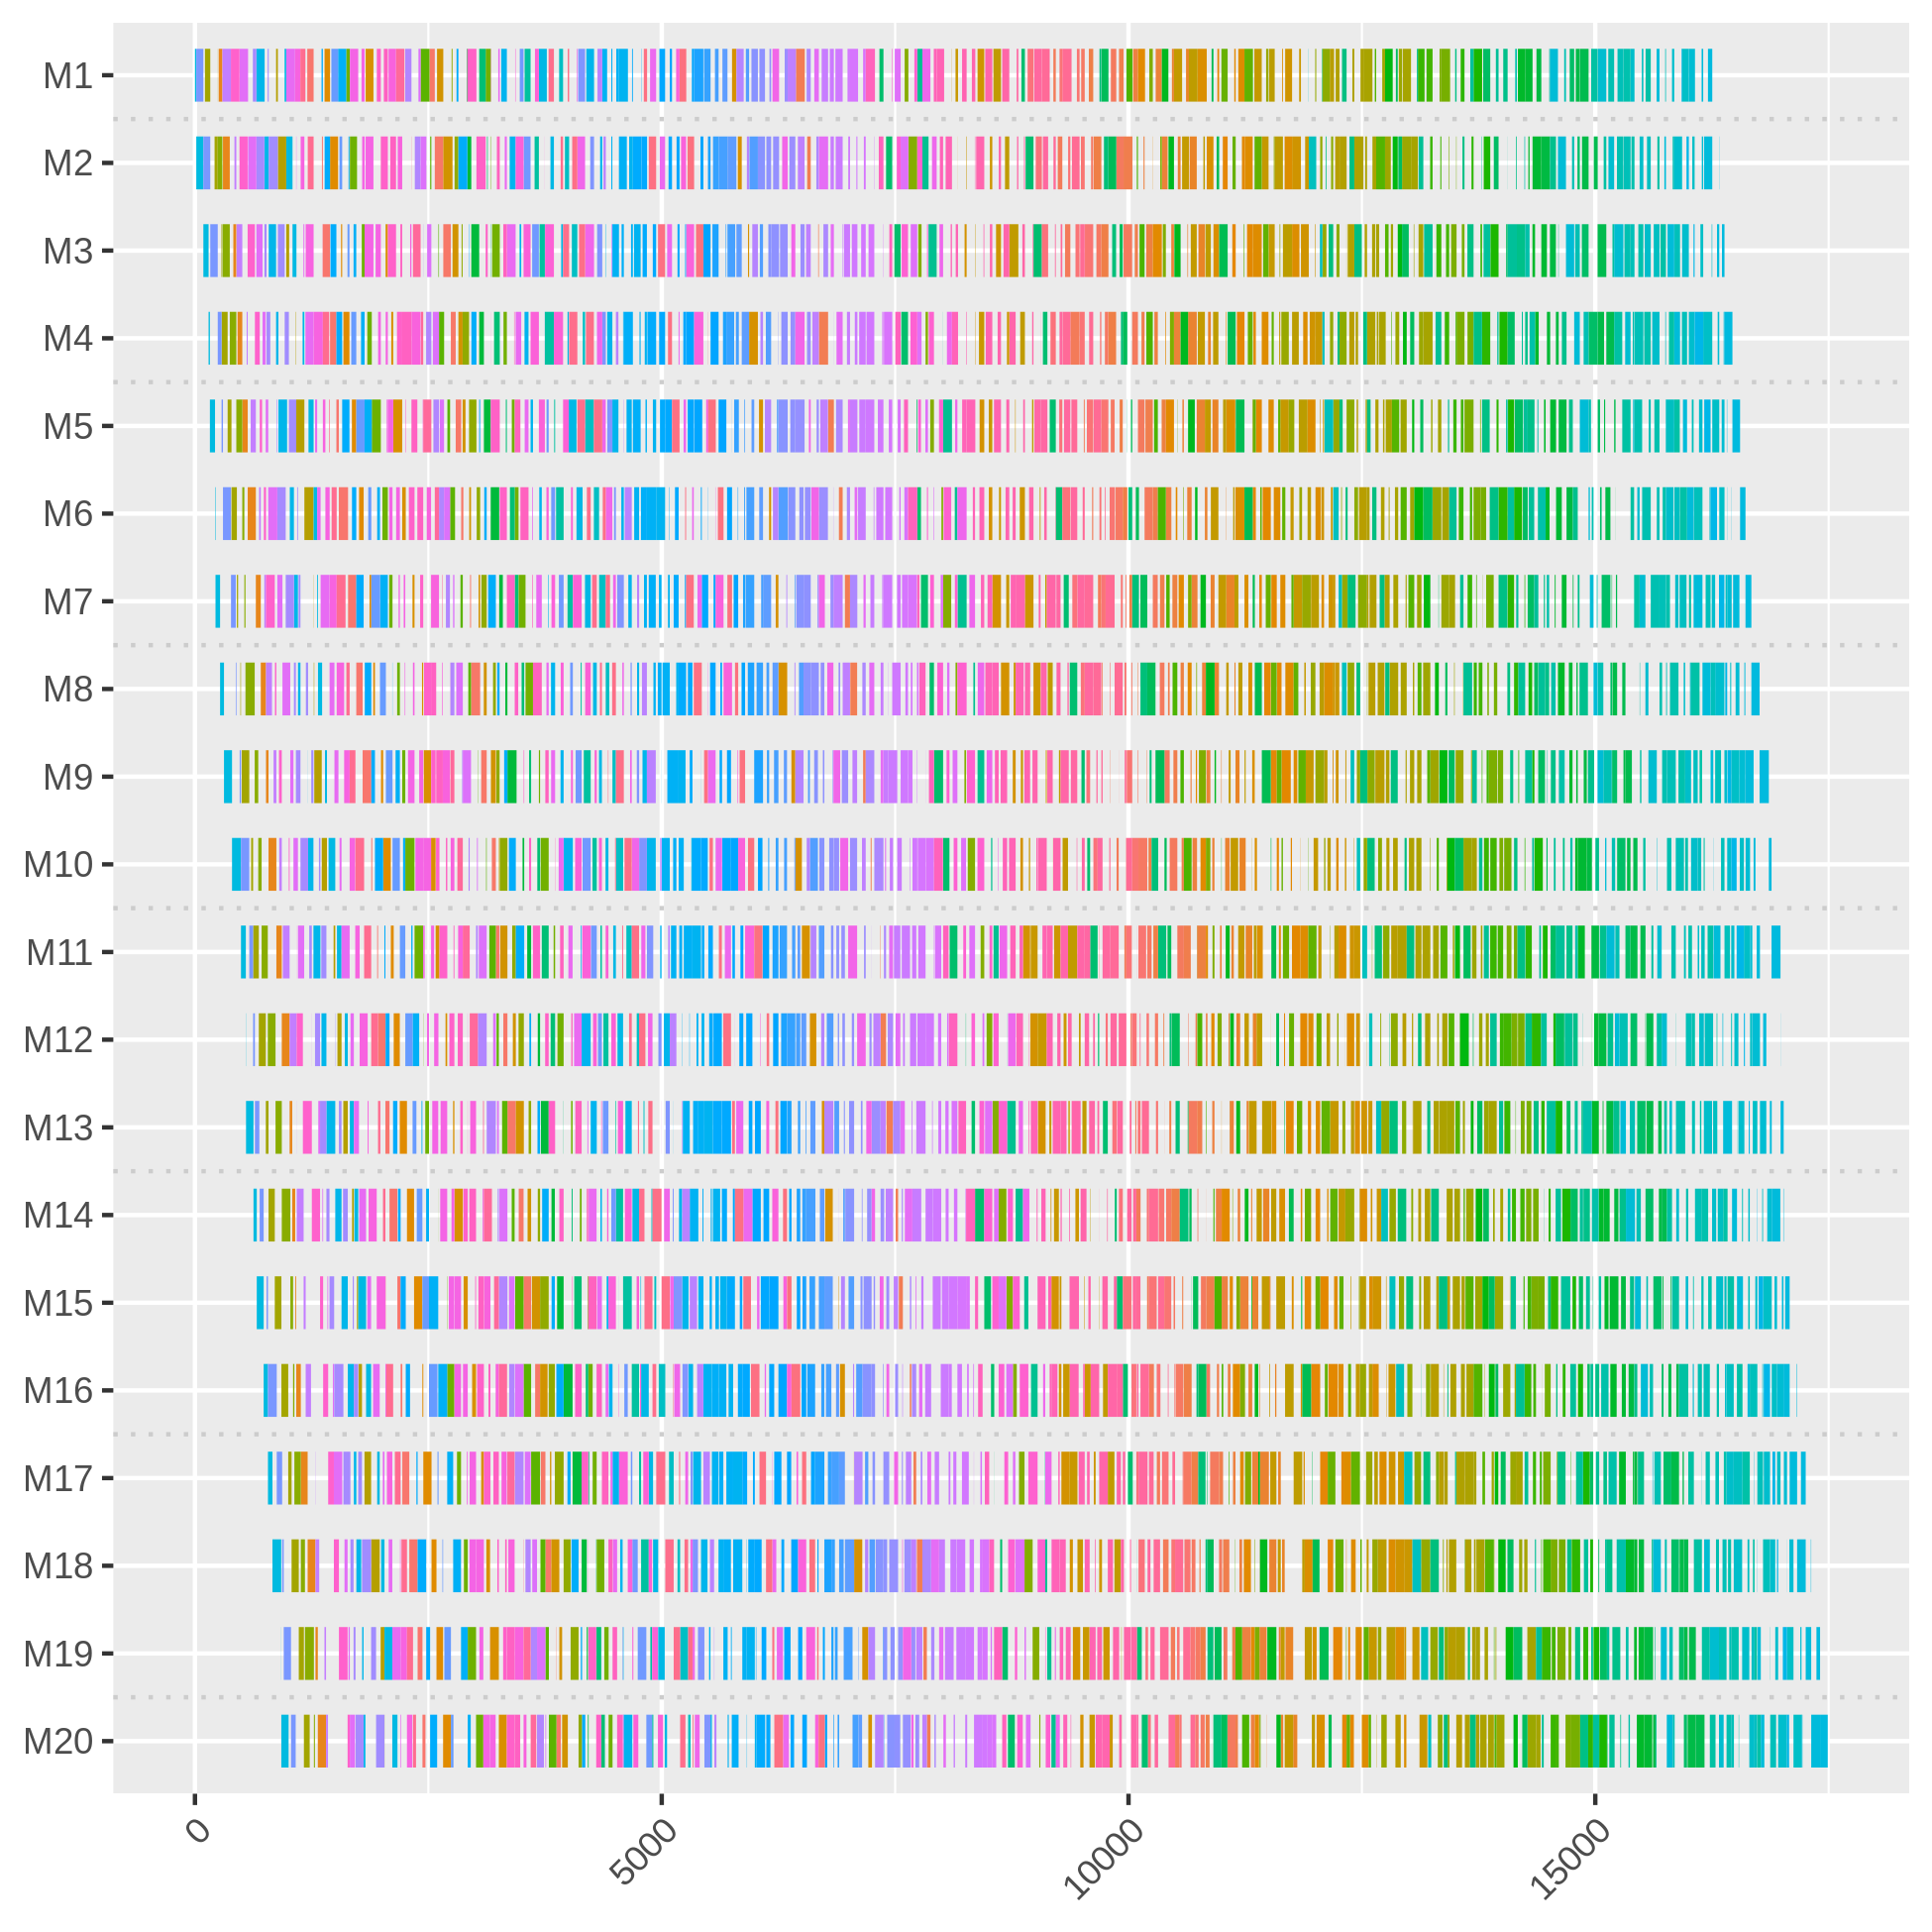
\includegraphics[width=\linewidth]{20_200_GC_2.png}
					\captionof{figure}{Gantt Chart for file 101.txt}
					
					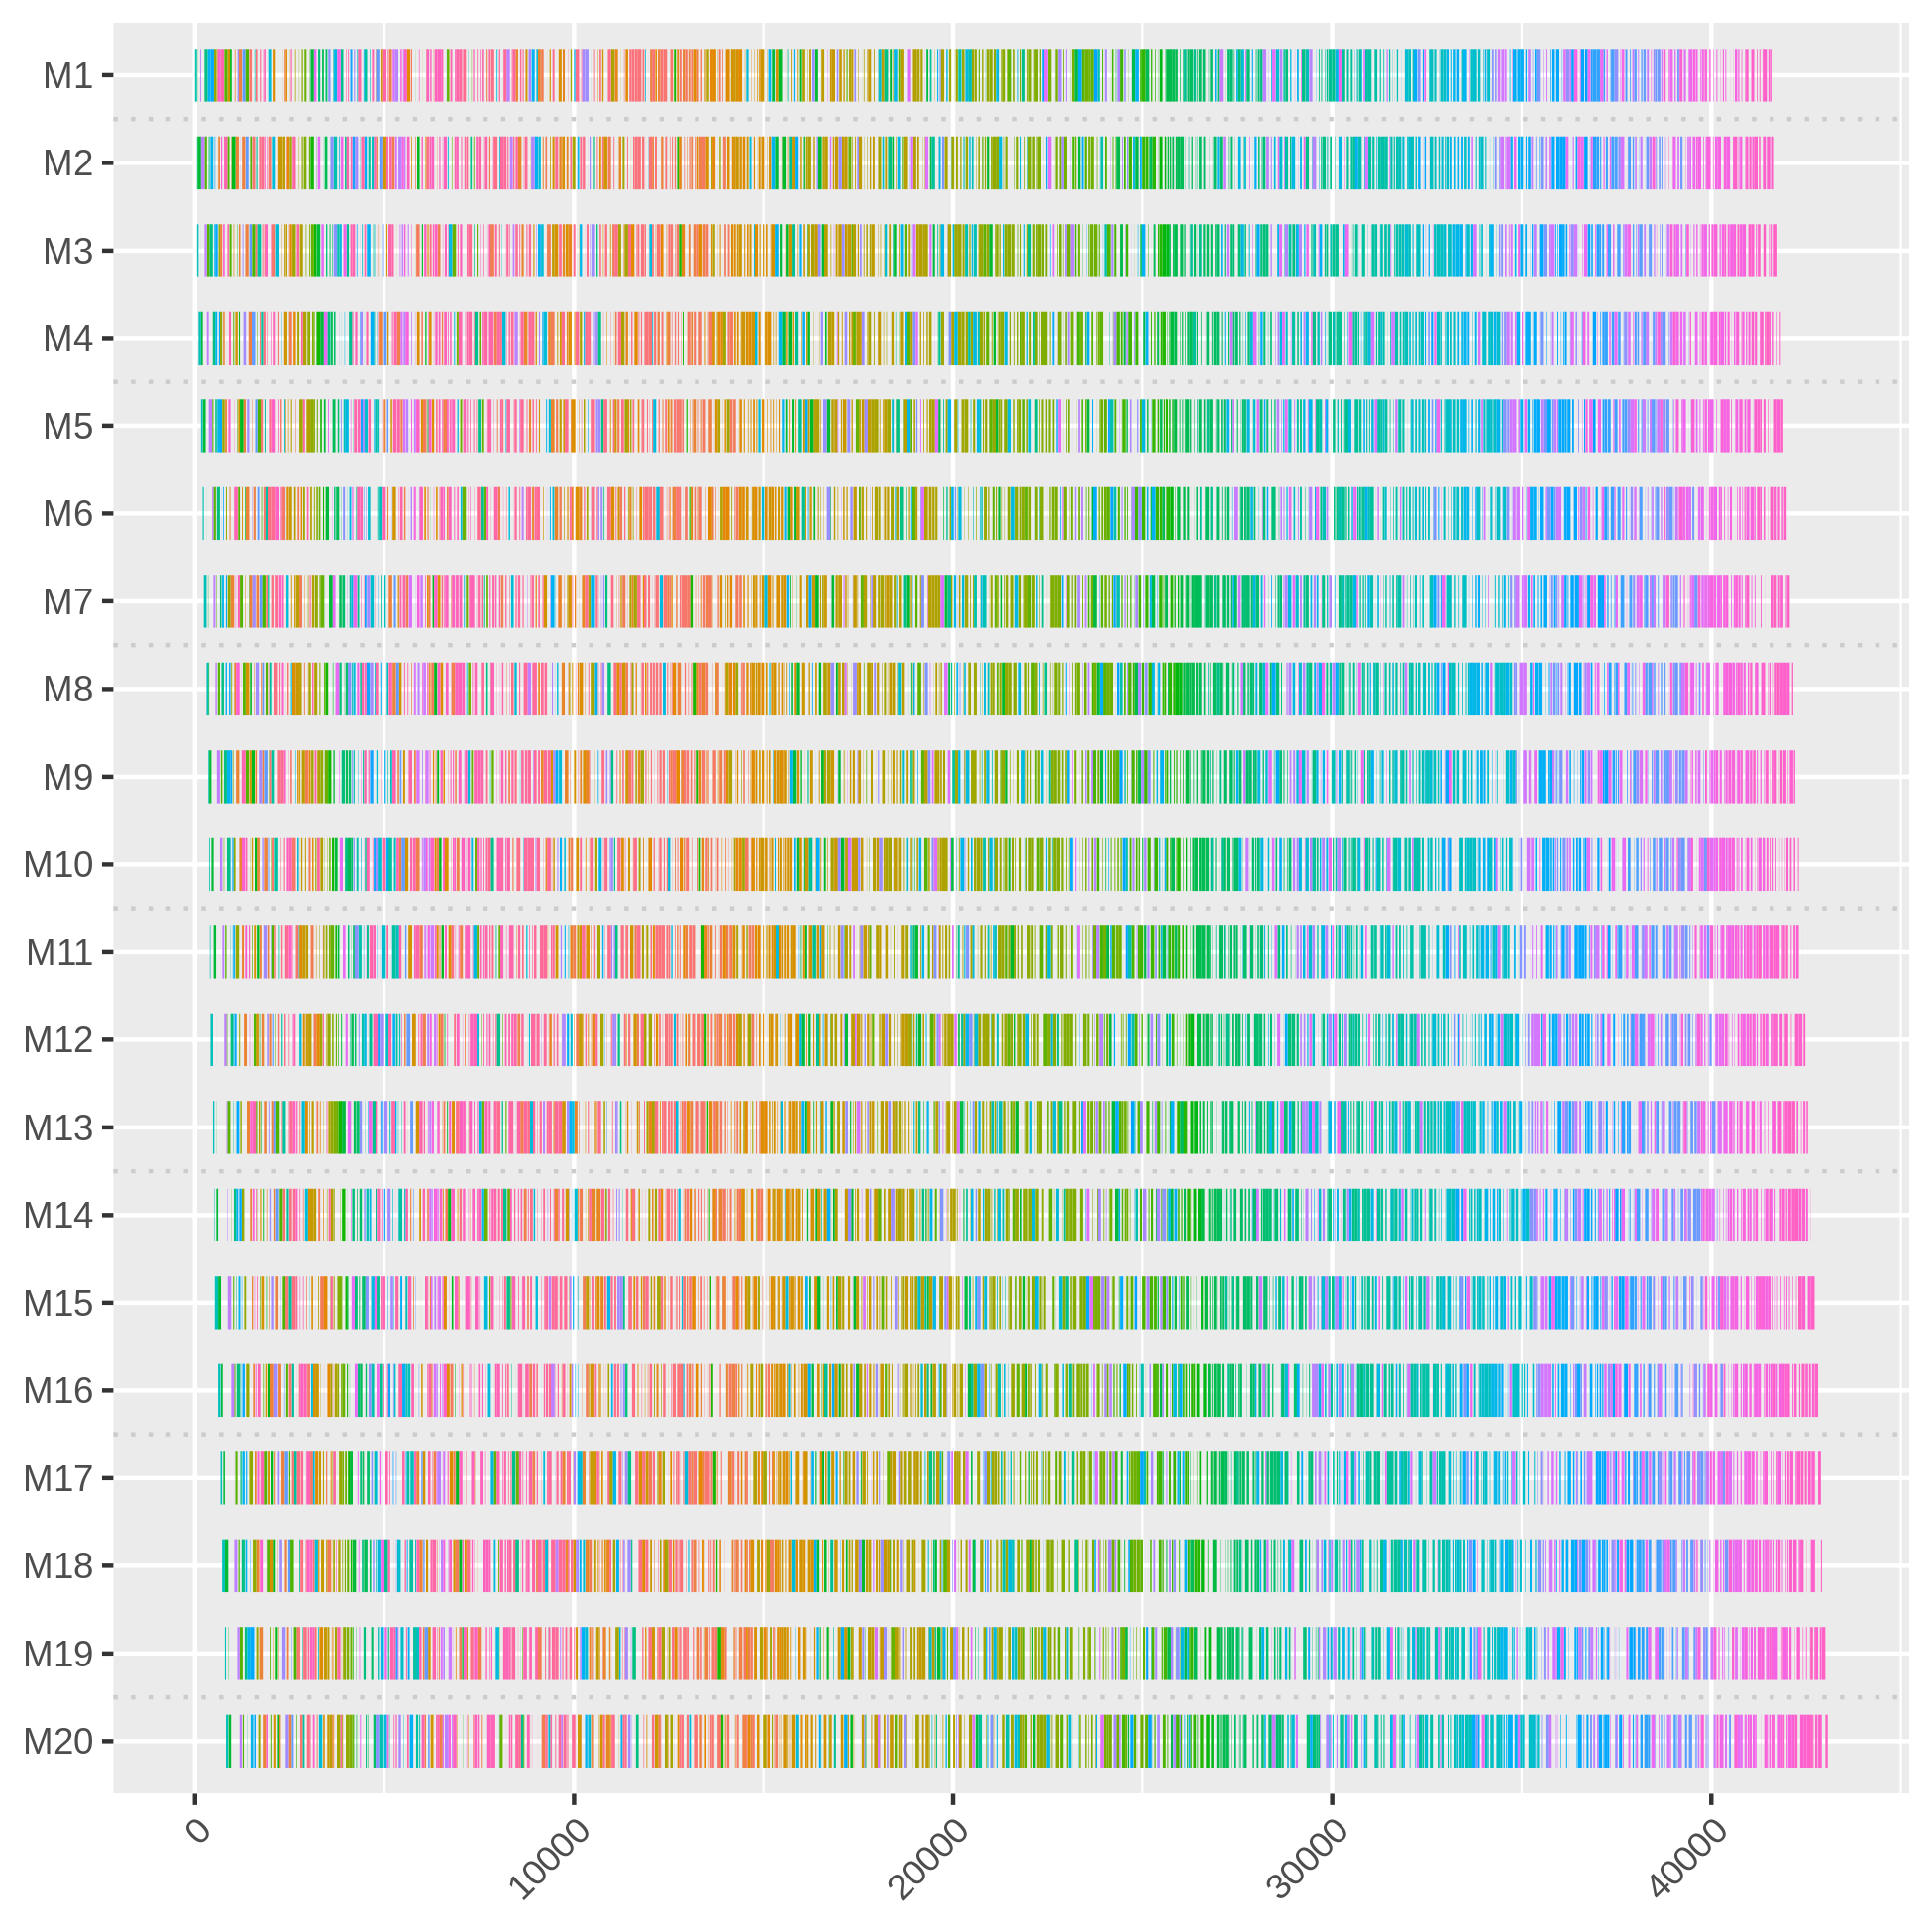
\includegraphics[width=\linewidth]{20_500_GC_2.png}
					\captionof{figure}{Gantt Chart for file 111.txt}
					
				\subsubsection{Results for Flow Shop Scheduling with Blocking}
					
					% latex table generated in R 3.6.0 by xtable 1.8-3 package
					% Fri May 31 14:40:56 2019
					\begin{table}[ht]
							\scalebox{0.9}{
								\begin{tabular}{rlrr}
									\hline
									& {\textbf{File.name}} & {\textbf{Best.makespan}} & {\textbf{\# func calls}} \\ 
									\hline
									{\textit{1}} & ../DataFiles/1.txt & 1459 & 558 \\ 
									{\textit{2}} & ../DataFiles/10.txt & 1420 & 568 \\ 
									{\textit{3}} & ../DataFiles/2.txt & 1501 & 554 \\ 
									{\textit{4}} & ../DataFiles/3.txt & 1447 & 565 \\ 
									{\textit{5}} & ../DataFiles/4.txt & 1608 & 567 \\ 
									{\textit{6}} & ../DataFiles/5.txt & 1472 & 565 \\ 
									{\textit{7}} & ../DataFiles/6.txt & 1526 & 559 \\ 
									{\textit{8}} & ../DataFiles/7.txt & 1485 &  62 \\ 
									{\textit{9}} & ../DataFiles/8.txt & 1495 &  61 \\ 
									{\textit{10}} & ../DataFiles/9.txt & 1521 &  59 \\ 
									{\textit{11}} & ../DataFiles/11.txt & 1876 & 568 \\ 
									{\textit{12}} & ../DataFiles/12.txt & 1957 & 565 \\ 
									{\textit{13}} & ../DataFiles/13.txt & 1828 & 566 \\ 
									{\textit{14}} & ../DataFiles/14.txt & 1726 & 569 \\ 
									{\textit{15}} & ../DataFiles/15.txt & 1849 & 564 \\ 
									{\textit{16}} & ../DataFiles/16.txt & 1776 & 562 \\ 
									{\textit{17}} & ../DataFiles/17.txt & 1865 & 563 \\ 
									{\textit{18}} & ../DataFiles/18.txt & 1946 & 568 \\ 
									{\textit{19}} & ../DataFiles/19.txt & 1962 & 569 \\ 
									{\textit{20}} & ../DataFiles/20.txt & 1942 & 566 \\ 
									{\textit{21}} & ../DataFiles/21.txt & 2640 & 570 \\ 
									{\textit{22}} & ../DataFiles/22.txt & 2386 & 570 \\ 
									{\textit{23}} & ../DataFiles/23.txt & 2666 & 567 \\ 
									{\textit{24}} & ../DataFiles/24.txt & 2641 & 568 \\ 
									{\textit{25}} & ../DataFiles/25.txt & 2708 & 570 \\ 
									{\textit{26}} & ../DataFiles/26.txt & 2554 & 569 \\ 
									{\textit{27}} & ../DataFiles/27.txt & 2611 & 569 \\ 
									{\textit{28}} & ../DataFiles/28.txt & 2413 & 570 \\ 
									{\textit{29}} & ../DataFiles/29.txt & 2650 & 568 \\ 
									{\textit{30}} & ../DataFiles/30.txt & 2572 & 568 \\ 
									{\textit{31}} & ../DataFiles/31.txt & 3429 & 3645 \\ 
									{\textit{32}} & ../DataFiles/32.txt & 3536 & 3653 \\ 
									{\textit{33}} & ../DataFiles/33.txt & 3356 & 3646 \\ 
									{\textit{34}} & ../DataFiles/34.txt & 3493 & 3654 \\ 
									{\textit{35}} & ../DataFiles/35.txt & 3564 & 3659 \\ 
									{\textit{36}} & ../DataFiles/36.txt & 3486 & 3654 \\ 
									{\textit{37}} & ../DataFiles/37.txt & 3317 & 3642 \\ 
									{\textit{38}} & ../DataFiles/38.txt & 3380 & 3666 \\ 
									{\textit{39}} & ../DataFiles/39.txt & 3163 & 3663 \\ 
									{\textit{40}} & ../DataFiles/40.txt & 3507 & 3646 \\ 
									{\textit{41}} & ../DataFiles/41.txt & 4164 & 3664 \\ 
									{\textit{42}} & ../DataFiles/42.txt & 3834 & 3663 \\ 
									{\textit{43}} & ../DataFiles/43.txt & 4028 & 3658 \\ 
									{\textit{44}} & ../DataFiles/44.txt & 4111 & 3670 \\ 
									{\textit{45}} & ../DataFiles/45.txt & 4099 & 3666 \\ 
									\hline
								\end{tabular}
							}
					\end{table}
				\clearpage
				\begin{table}[ht]
						\scalebox{0.9}{
							\begin{tabular}{rlrr}
								\hline
								& {\textbf{File.name}} & {\textbf{Best.makespan}} & {\textbf{\# func calls}} \\ 
								\hline
								{\textit{1}} & ../DataFiles/46.txt & 3985 & 3664 \\ 
								{\textit{2}} & ../DataFiles/47.txt & 4062 & 3655 \\ 
								{\textit{3}} & ../DataFiles/48.txt & 3879 & 3650 \\ 
								{\textit{4}} & ../DataFiles/49.txt & 3837 & 3661 \\ 
								{\textit{5}} & ../DataFiles/50.txt & 3967 & 3653 \\ 
								{\textit{6}} & ../DataFiles/51.txt & 4961 & 3601 \\ 
								{\textit{7}} & ../DataFiles/52.txt & 4672 & 3648 \\ 
								{\textit{8}} & ../DataFiles/53.txt & 4830 & 3630 \\ 
								{\textit{9}} & ../DataFiles/54.txt & 4721 & 3664 \\ 
								{\textit{10}} & ../DataFiles/55.txt & 4863 & 3664 \\ 
								{\textit{11}} & ../DataFiles/56.txt & 4711 & 3664 \\ 
								{\textit{12}} & ../DataFiles/57.txt & 4867 & 3634 \\ 
								{\textit{13}} & ../DataFiles/58.txt & 4803 & 3610 \\ 
								{\textit{14}} & ../DataFiles/59.txt & 4760 & 3666 \\ 
								{\textit{15}} & ../DataFiles/60.txt & 4907 & 3664 \\ 
								{\textit{16}} & ../DataFiles/61.txt & 6917 & 14807 \\ 
								{\textit{17}} & ../DataFiles/62.txt & 6551 & 14805 \\ 
								{\textit{18}} & ../DataFiles/63.txt & 6585 & 14788 \\ 
								{\textit{19}} & ../DataFiles/64.txt & 6356 & 14753 \\ 
								{\textit{20}} & ../DataFiles/65.txt & 6629 & 14785 \\ 
								{\textit{21}} & ../DataFiles/66.txt & 6470 & 14775 \\ 
								{\textit{22}} & ../DataFiles/67.txt & 6637 & 14792 \\ 
								{\textit{23}} & ../DataFiles/68.txt & 6504 & 14763 \\ 
								{\textit{24}} & ../DataFiles/69.txt & 6741 & 14801 \\ 
								{\textit{25}} & ../DataFiles/70.txt & 6748 & 14765 \\ 
								{\textit{26}} & ../DataFiles/71.txt & 7769 & 14798 \\ 
								{\textit{27}} & ../DataFiles/72.txt & 7469 & 14795 \\ 
								{\textit{28}} & ../DataFiles/73.txt & 7610 & 14784 \\ 
								{\textit{29}} & ../DataFiles/74.txt & 7775 & 14758 \\ 
								{\textit{30}} & ../DataFiles/75.txt & 7627 & 14785 \\ 
								{\textit{31}} & ../DataFiles/76.txt & 7413 & 14786 \\ 
								{\textit{32}} & ../DataFiles/77.txt & 7463 & 14770 \\ 
								{\textit{33}} & ../DataFiles/78.txt & 7664 & 14469 \\ 
								{\textit{34}} & ../DataFiles/79.txt & 7802 & 14541 \\ 
								{\textit{35}} & ../DataFiles/80.txt & 7608 & 14695 \\ 
								{\textit{36}} & ../DataFiles/81.txt & 8441 & 14562 \\ 
								{\textit{37}} & ../DataFiles/82.txt & 8652 & 14350 \\ 
								{\textit{38}} & ../DataFiles/83.txt & 8757 & 14751 \\ 
								{\textit{39}} & ../DataFiles/84.txt & 8536 & 14709 \\ 
								{\textit{40}} & ../DataFiles/85.txt & 8683 & 14751 \\ 
								{\textit{41}} & ../DataFiles/86.txt & 8533 & 14515 \\ 
								{\textit{42}} & ../DataFiles/87.txt & 8608 & 14754 \\ 
								{\textit{43}} & ../DataFiles/88.txt & 8711 & 14578 \\ 
								{\textit{44}} & ../DataFiles/89.txt & 8581 & 14495 \\ 
								{\textit{45}} & ../DataFiles/90.txt & 8675 & 14736 \\ 
								{\textit{46}} & ../DataFiles/100.txt & 14786 & 58742 \\ 
								\hline
							\end{tabular}
						}
				\end{table}
				\clearpage
				\begin{table}[ht]
						\scalebox{0.9}{
							\begin{tabular}{rlrr}
								\hline
								& {\textbf{File.name}} & {\textbf{Best.makespan}} & {\textbf{\# func calls}} \\ 
								\hline
								{\textit{1}} & ../DataFiles/91.txt & 14734 & 57677 \\ 
								{\textit{2}} & ../DataFiles/92.txt & 14792 & 59020 \\ 
								{\textit{3}} & ../DataFiles/93.txt & 14937 & 58896 \\ 
								{\textit{4}} & ../DataFiles/94.txt & 14838 & 58610 \\ 
								{\textit{5}} & ../DataFiles/95.txt & 14722 & 58556 \\ 
								{\textit{6}} & ../DataFiles/96.txt & 14513 & 58662 \\ 
								{\textit{7}} & ../DataFiles/97.txt & 14802 & 58847 \\ 
								{\textit{8}} & ../DataFiles/98.txt & 14989 & 58235 \\ 
								{\textit{9}} & ../DataFiles/99.txt & 14696 & 59014 \\ 
								{\textit{10}} & ../DataFiles/101.txt & 15995 & 58936 \\ 
								{\textit{11}} & ../DataFiles/102.txt & 16268 & 58787 \\ 
								{\textit{12}} & ../DataFiles/103.txt & 16482 & 58806 \\ 
								{\textit{13}} & ../DataFiles/104.txt & 16348 & 58975 \\ 
								{\textit{14}} & ../DataFiles/105.txt & 16157 & 58951 \\ 
								{\textit{15}} & ../DataFiles/106.txt & 16132 & 58804 \\ 
								{\textit{16}} & ../DataFiles/107.txt & 16297 & 58903 \\ 
								{\textit{17}} & ../DataFiles/108.txt & 16268 & 58752 \\ 
								{\textit{18}} & ../DataFiles/109.txt & 16230 & 58960 \\ 
								{\textit{19}} & ../DataFiles/110.txt & 16306 & 59090 \\ 
								{\textit{20}} & ../DataFiles/111.txt & 39101 & 370915 \\ 
								{\textit{21}} & ../DataFiles/112.txt & 39163 & 370431 \\ 
								{\textit{22}} & ../DataFiles/113.txt & 39046 & 370045 \\ 
								{\textit{23}} & ../DataFiles/114.txt & 39260 & 370815 \\ 
								{\textit{24}} & ../DataFiles/115.txt & 38970 & 370413 \\ 
								{\textit{25}} & ../DataFiles/116.txt & 39389 & 371219 \\ 
								{\textit{26}} & ../DataFiles/117.txt & 38974 & 370676 \\ 
								{\textit{27}} & ../DataFiles/118.txt & 39075 & 372572 \\ 
								{\textit{28}} & ../DataFiles/119.txt & 39191 & 372435 \\ 
								{\textit{29}} & ../DataFiles/120.txt & 39396 & 372202 \\ 
								\hline
							\end{tabular}
						}
					\caption{Results for Flow Shop Scheduling with Blocking}
				\end{table}
			
			\subsubsection{Analysis}
				As seen from table1 above, both the makespan and the number of function calls increases as the number of machines or the number of jobs increases. Here results could not be compared to those on Taillard's website as the algorithm used to compute the makespan is different.
					
			\subsection{Flow Shop Scheduling with No Wait}
				\subsubsection{Gantt Charts}
				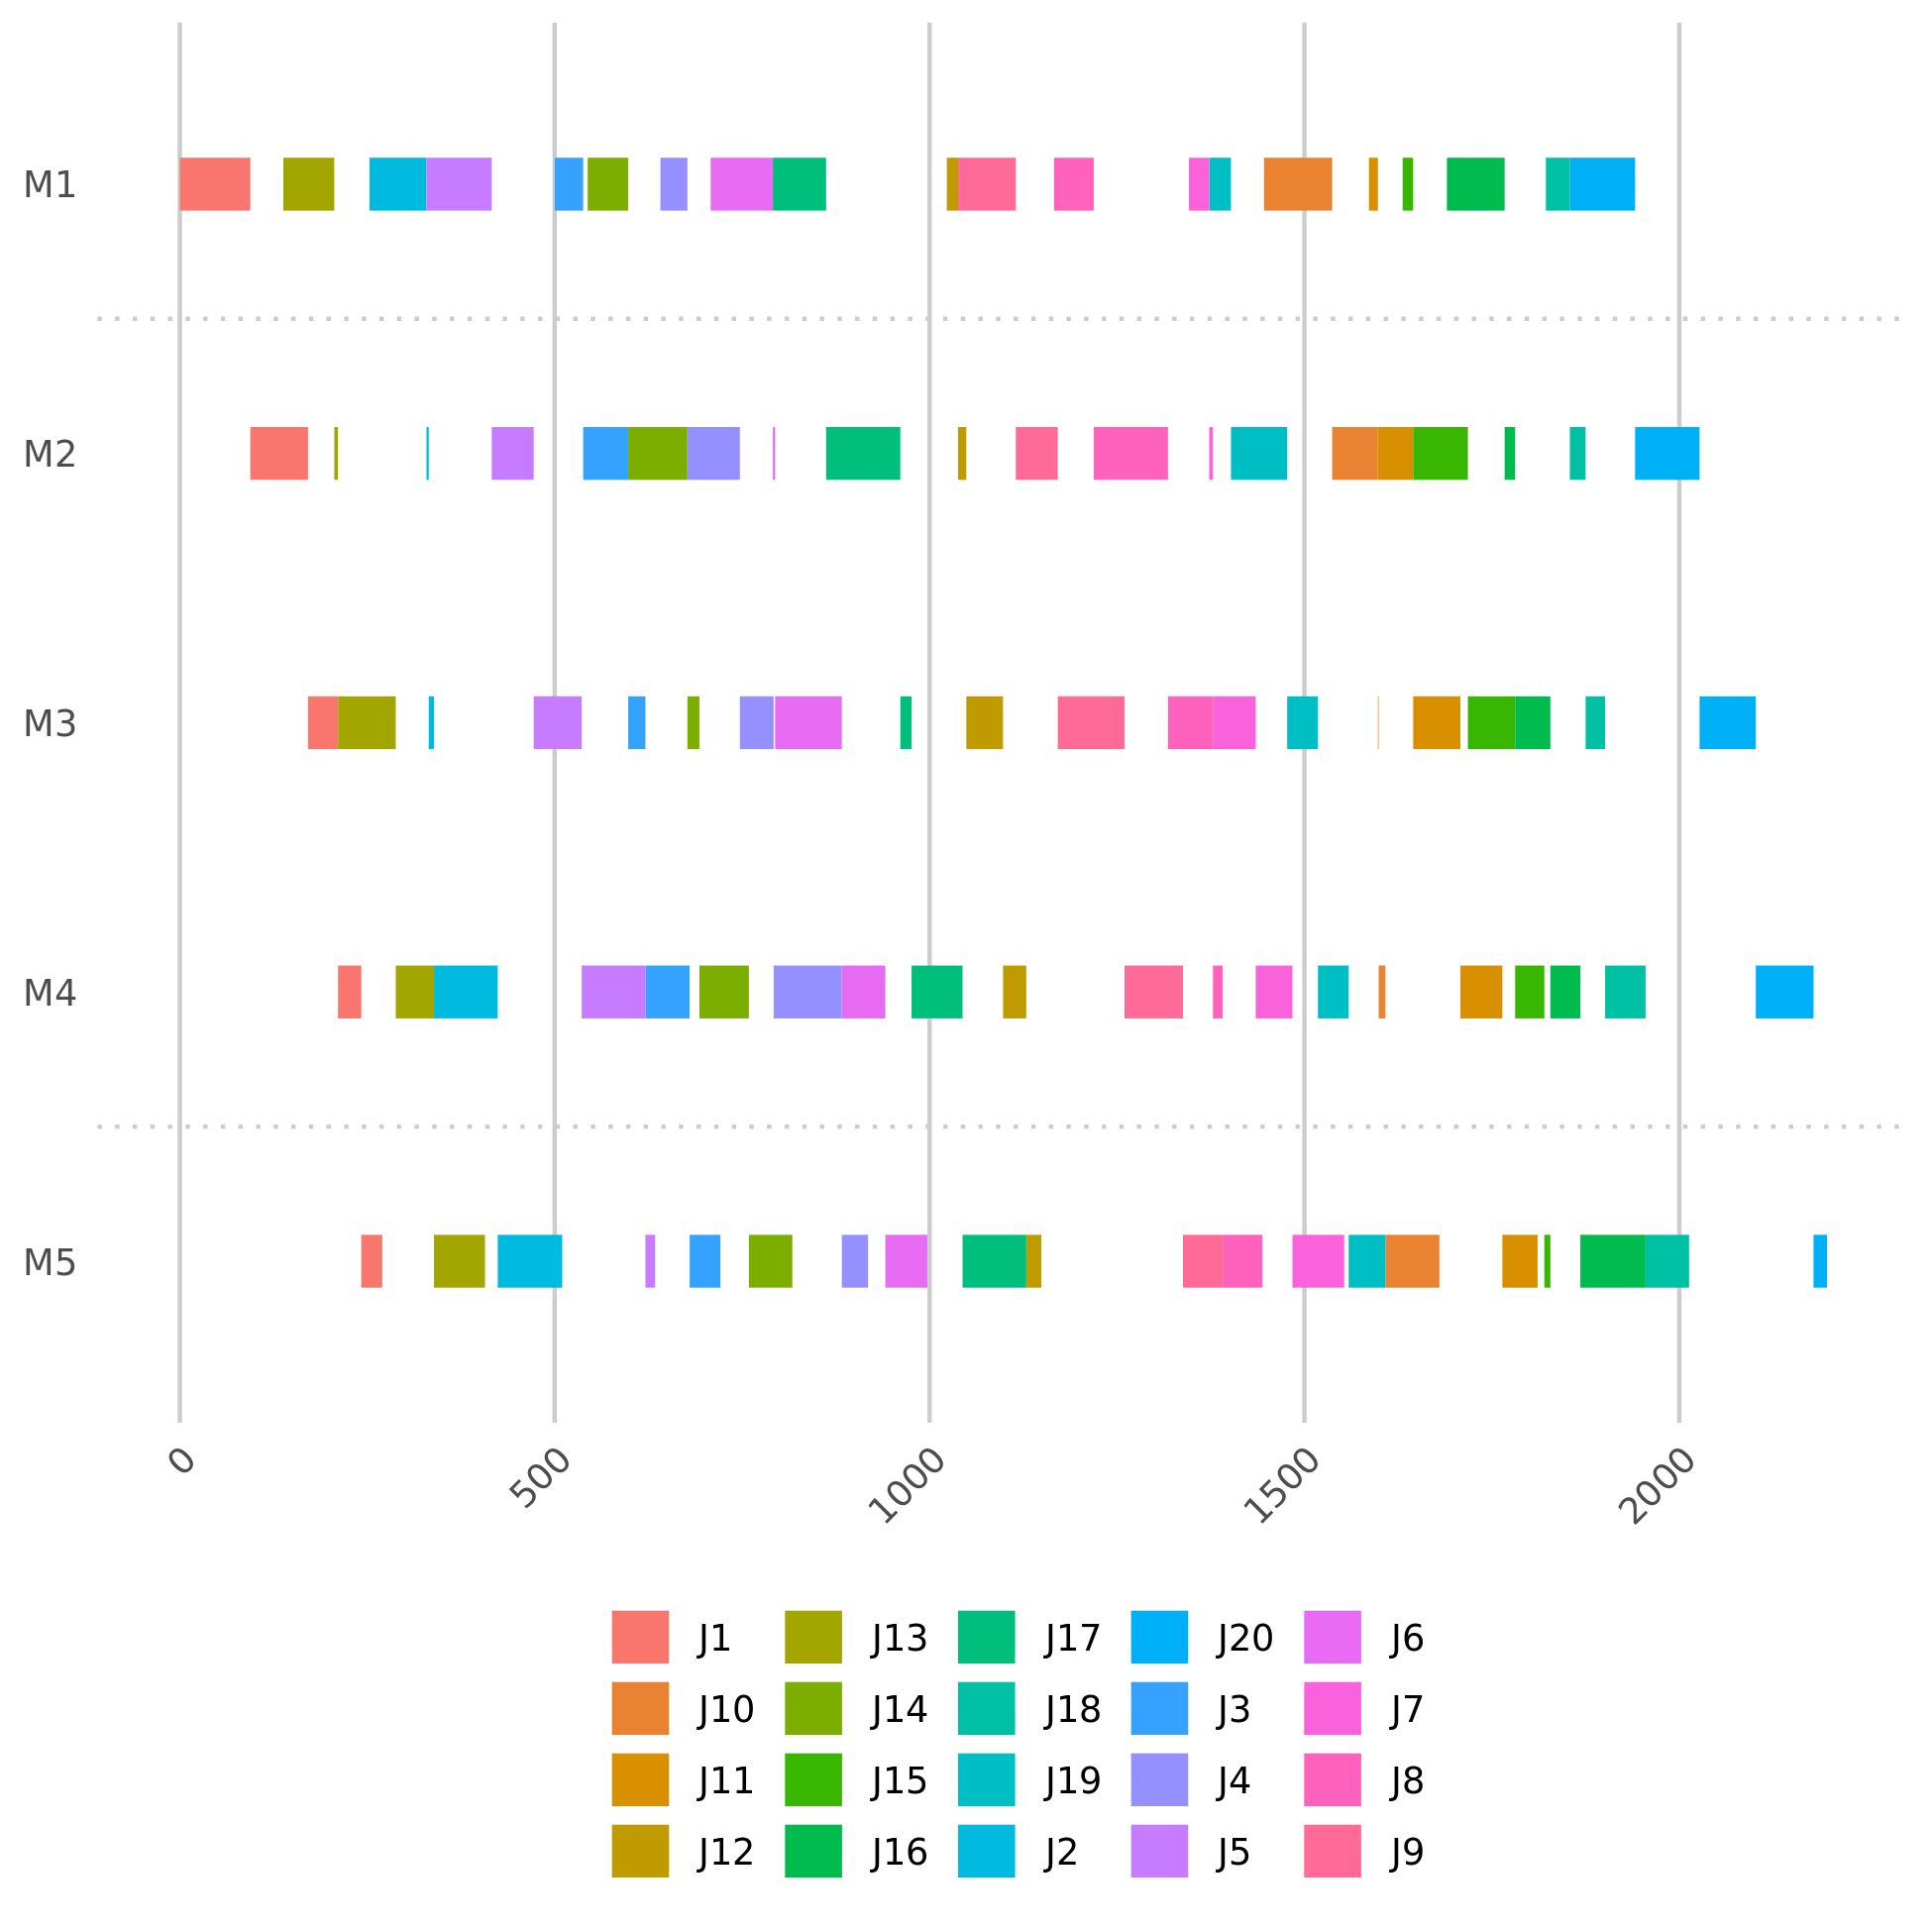
\includegraphics[width=\linewidth]{5_20_GC_3.png}
				\captionof{figure}{Gantt Chart for file 1.txt}
				
				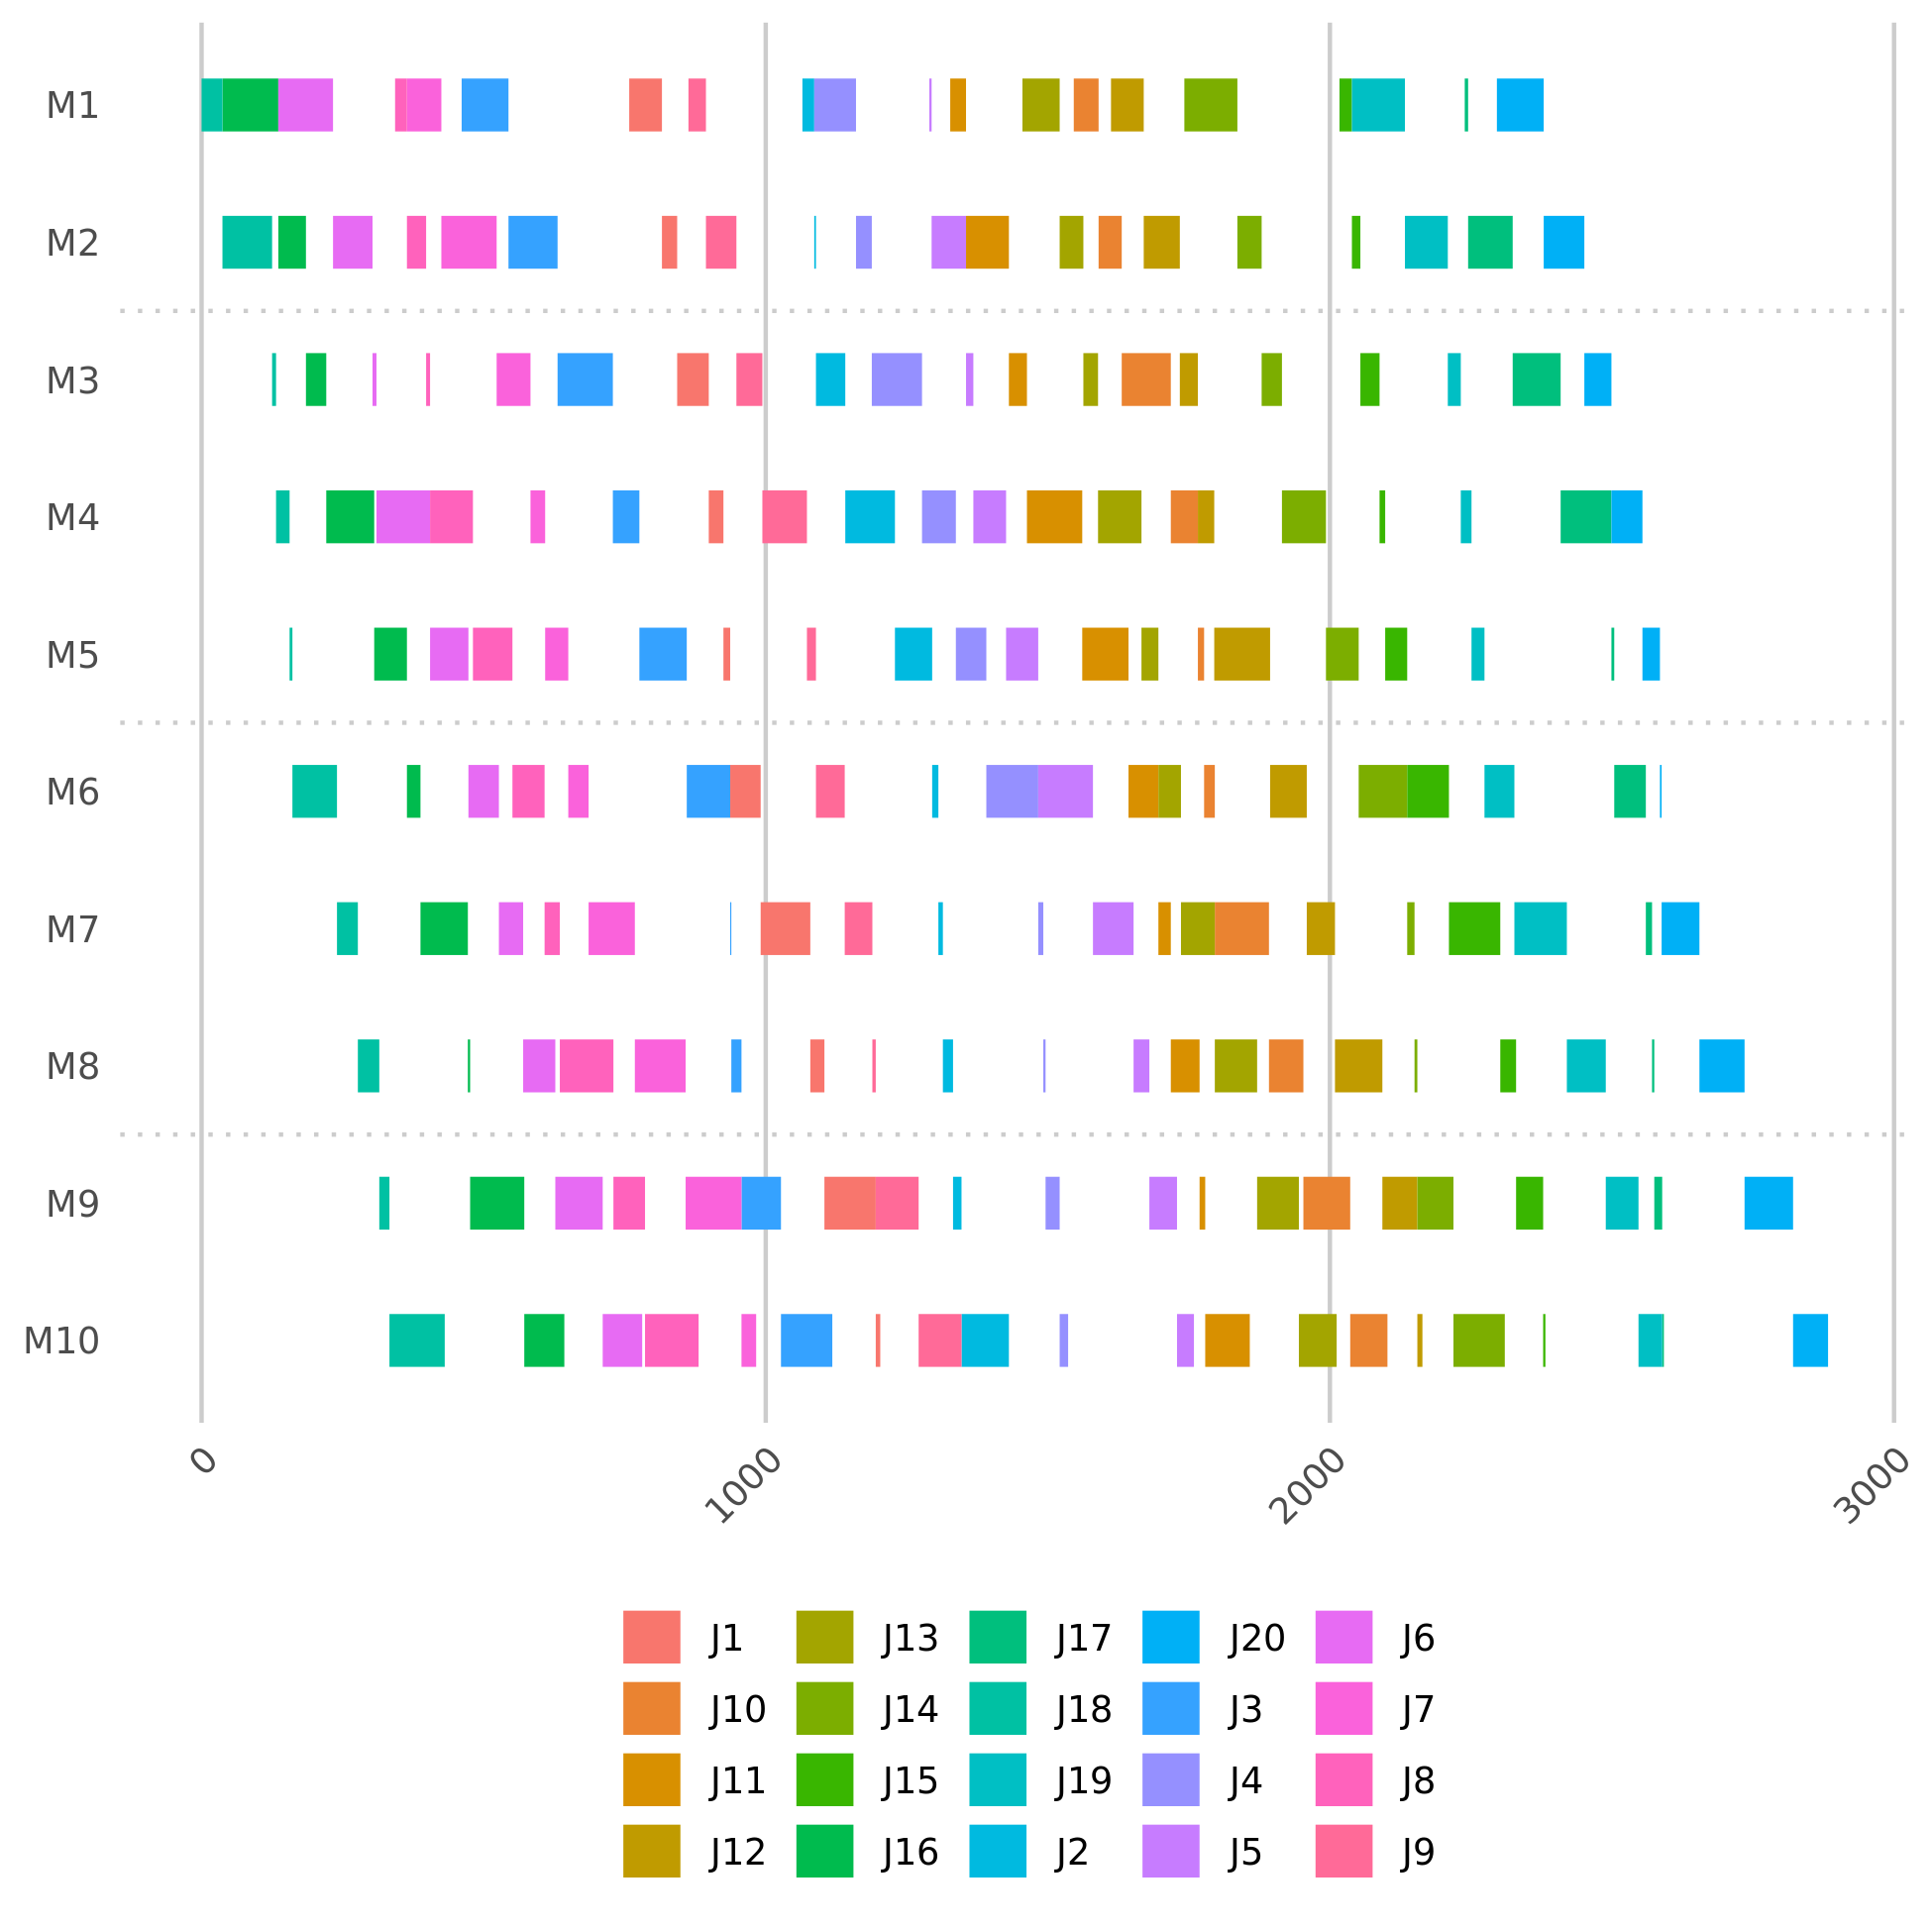
\includegraphics[width=\linewidth]{10_20_GC_3.png}
				\captionof{figure}{Gantt Chart for file 11.txt}
				
				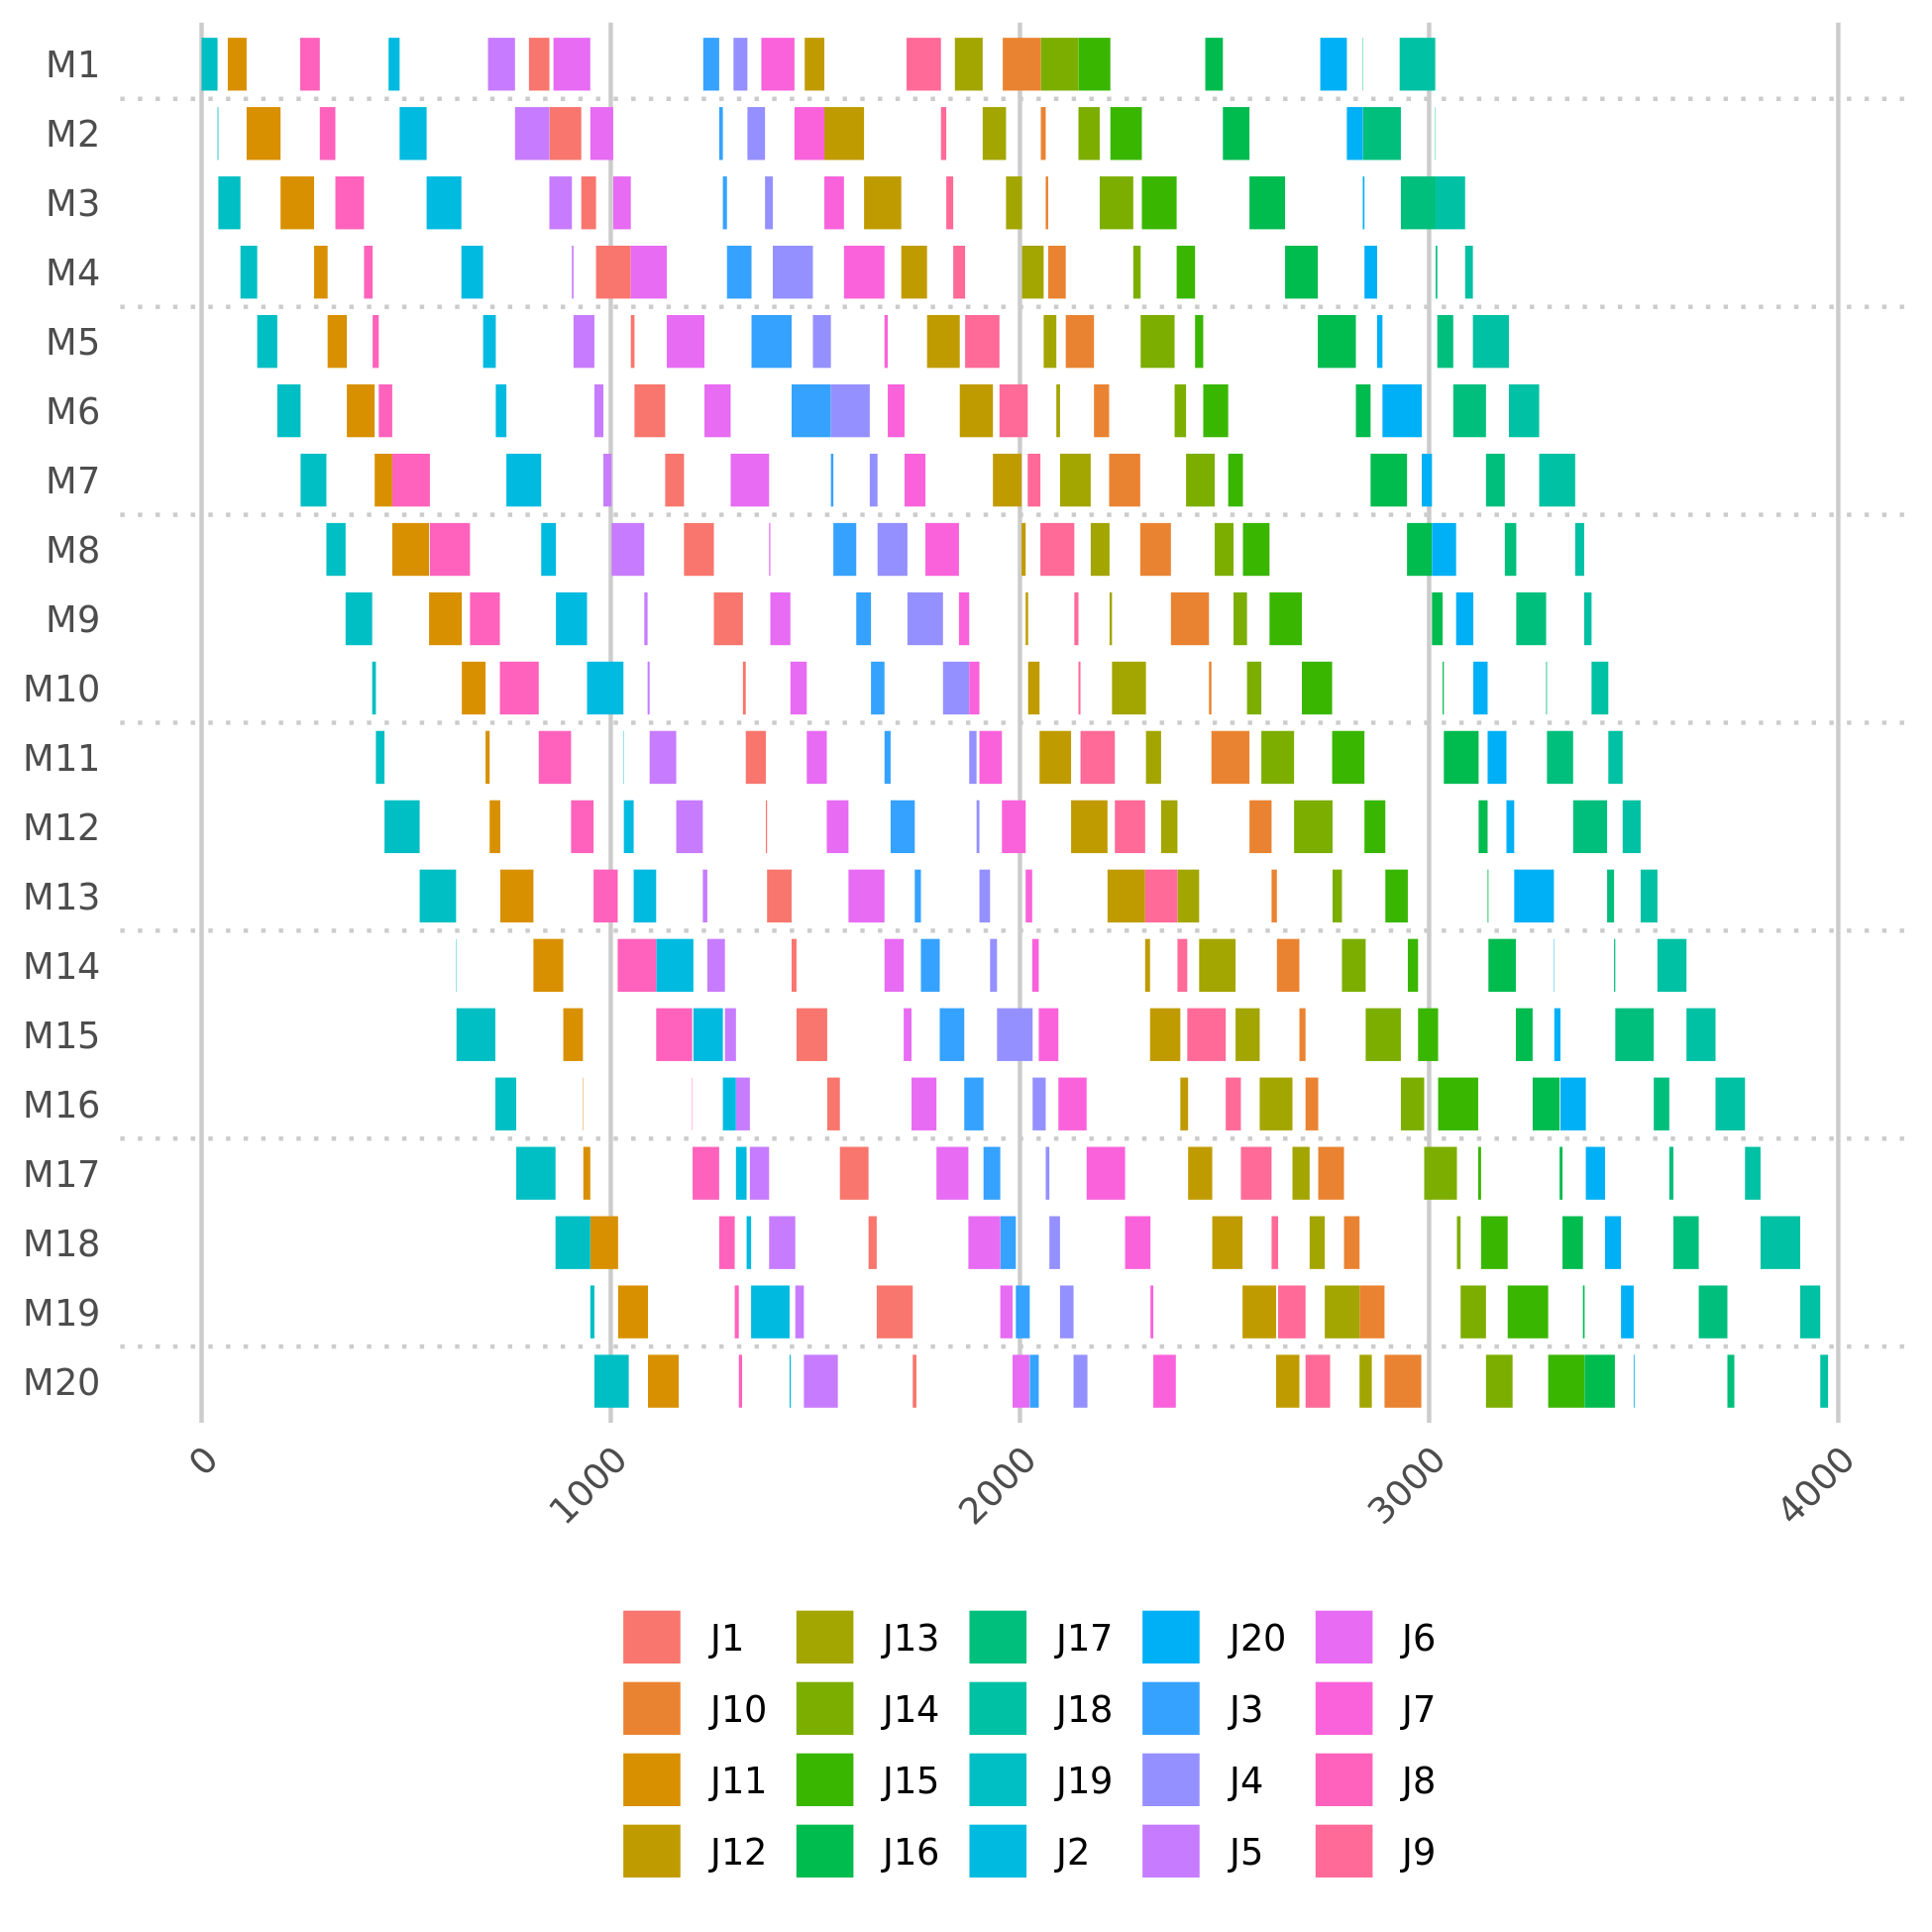
\includegraphics[width=\linewidth]{20_20_GC_3.png}
				\captionof{figure}{Gantt Chart for file 21.txt}
				
				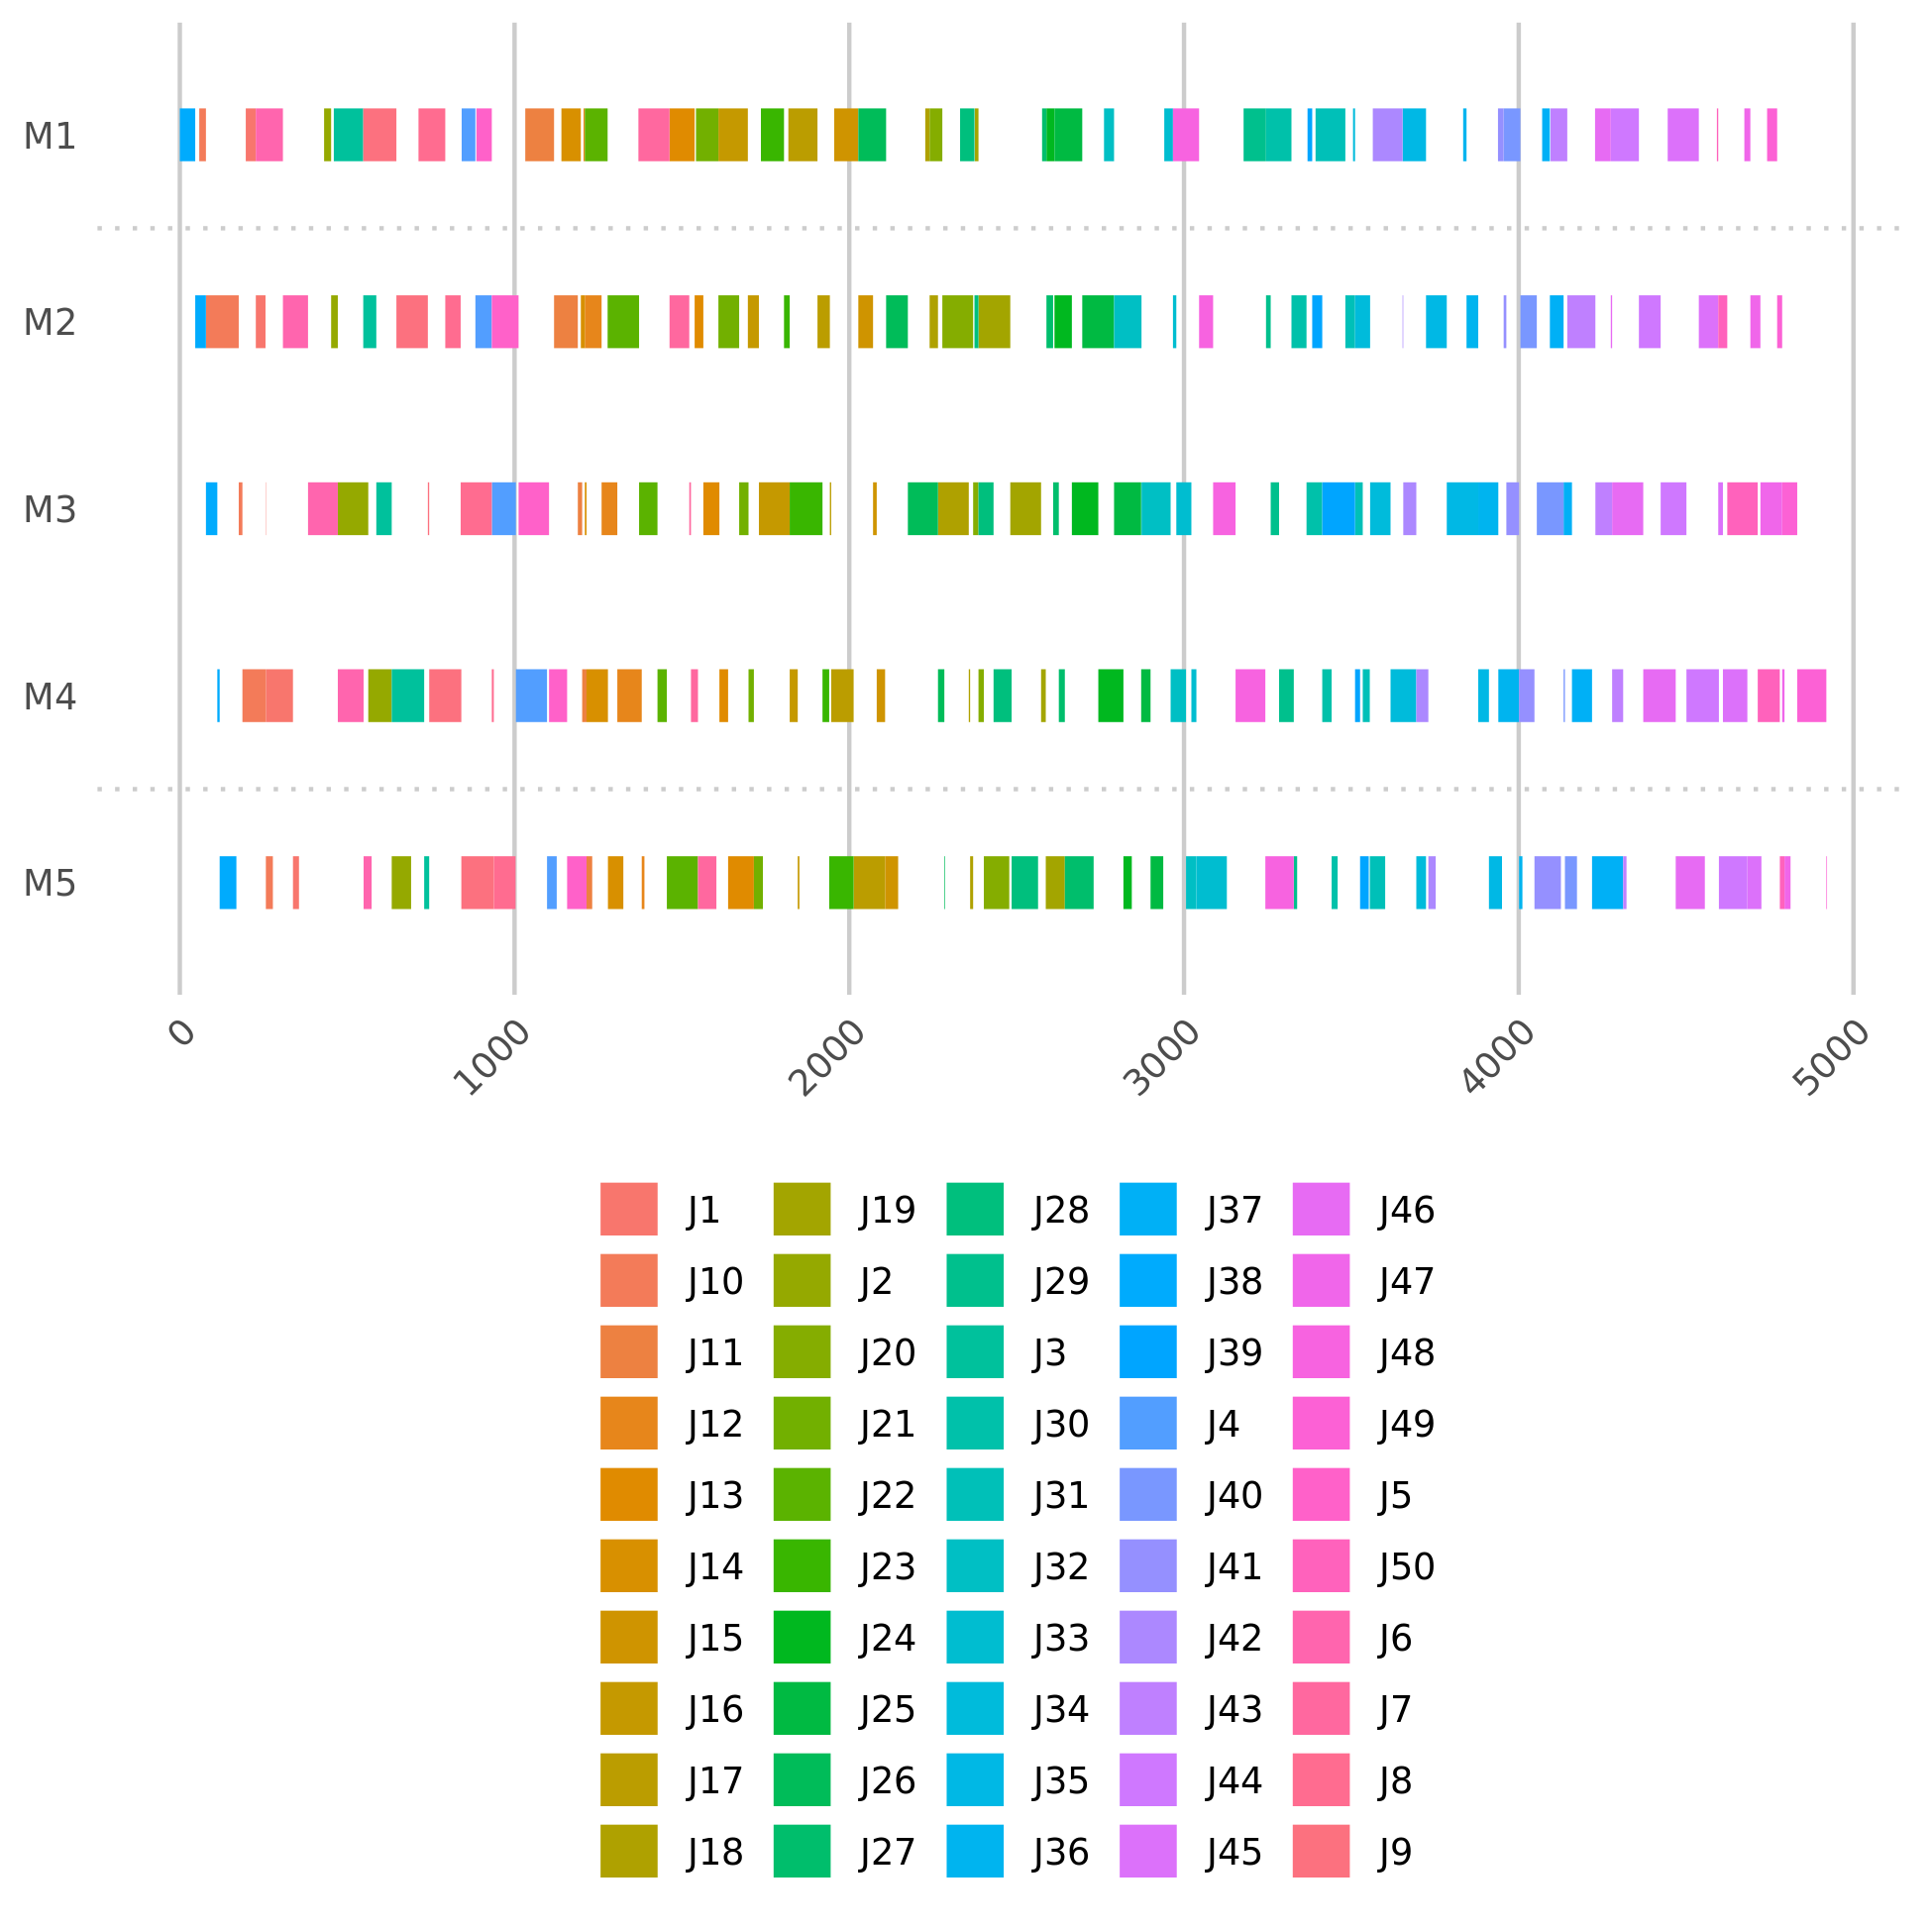
\includegraphics[width=\linewidth]{5_50_GC_3.png}
				\captionof{figure}{Gantt Chart for file 31.txt}
				
				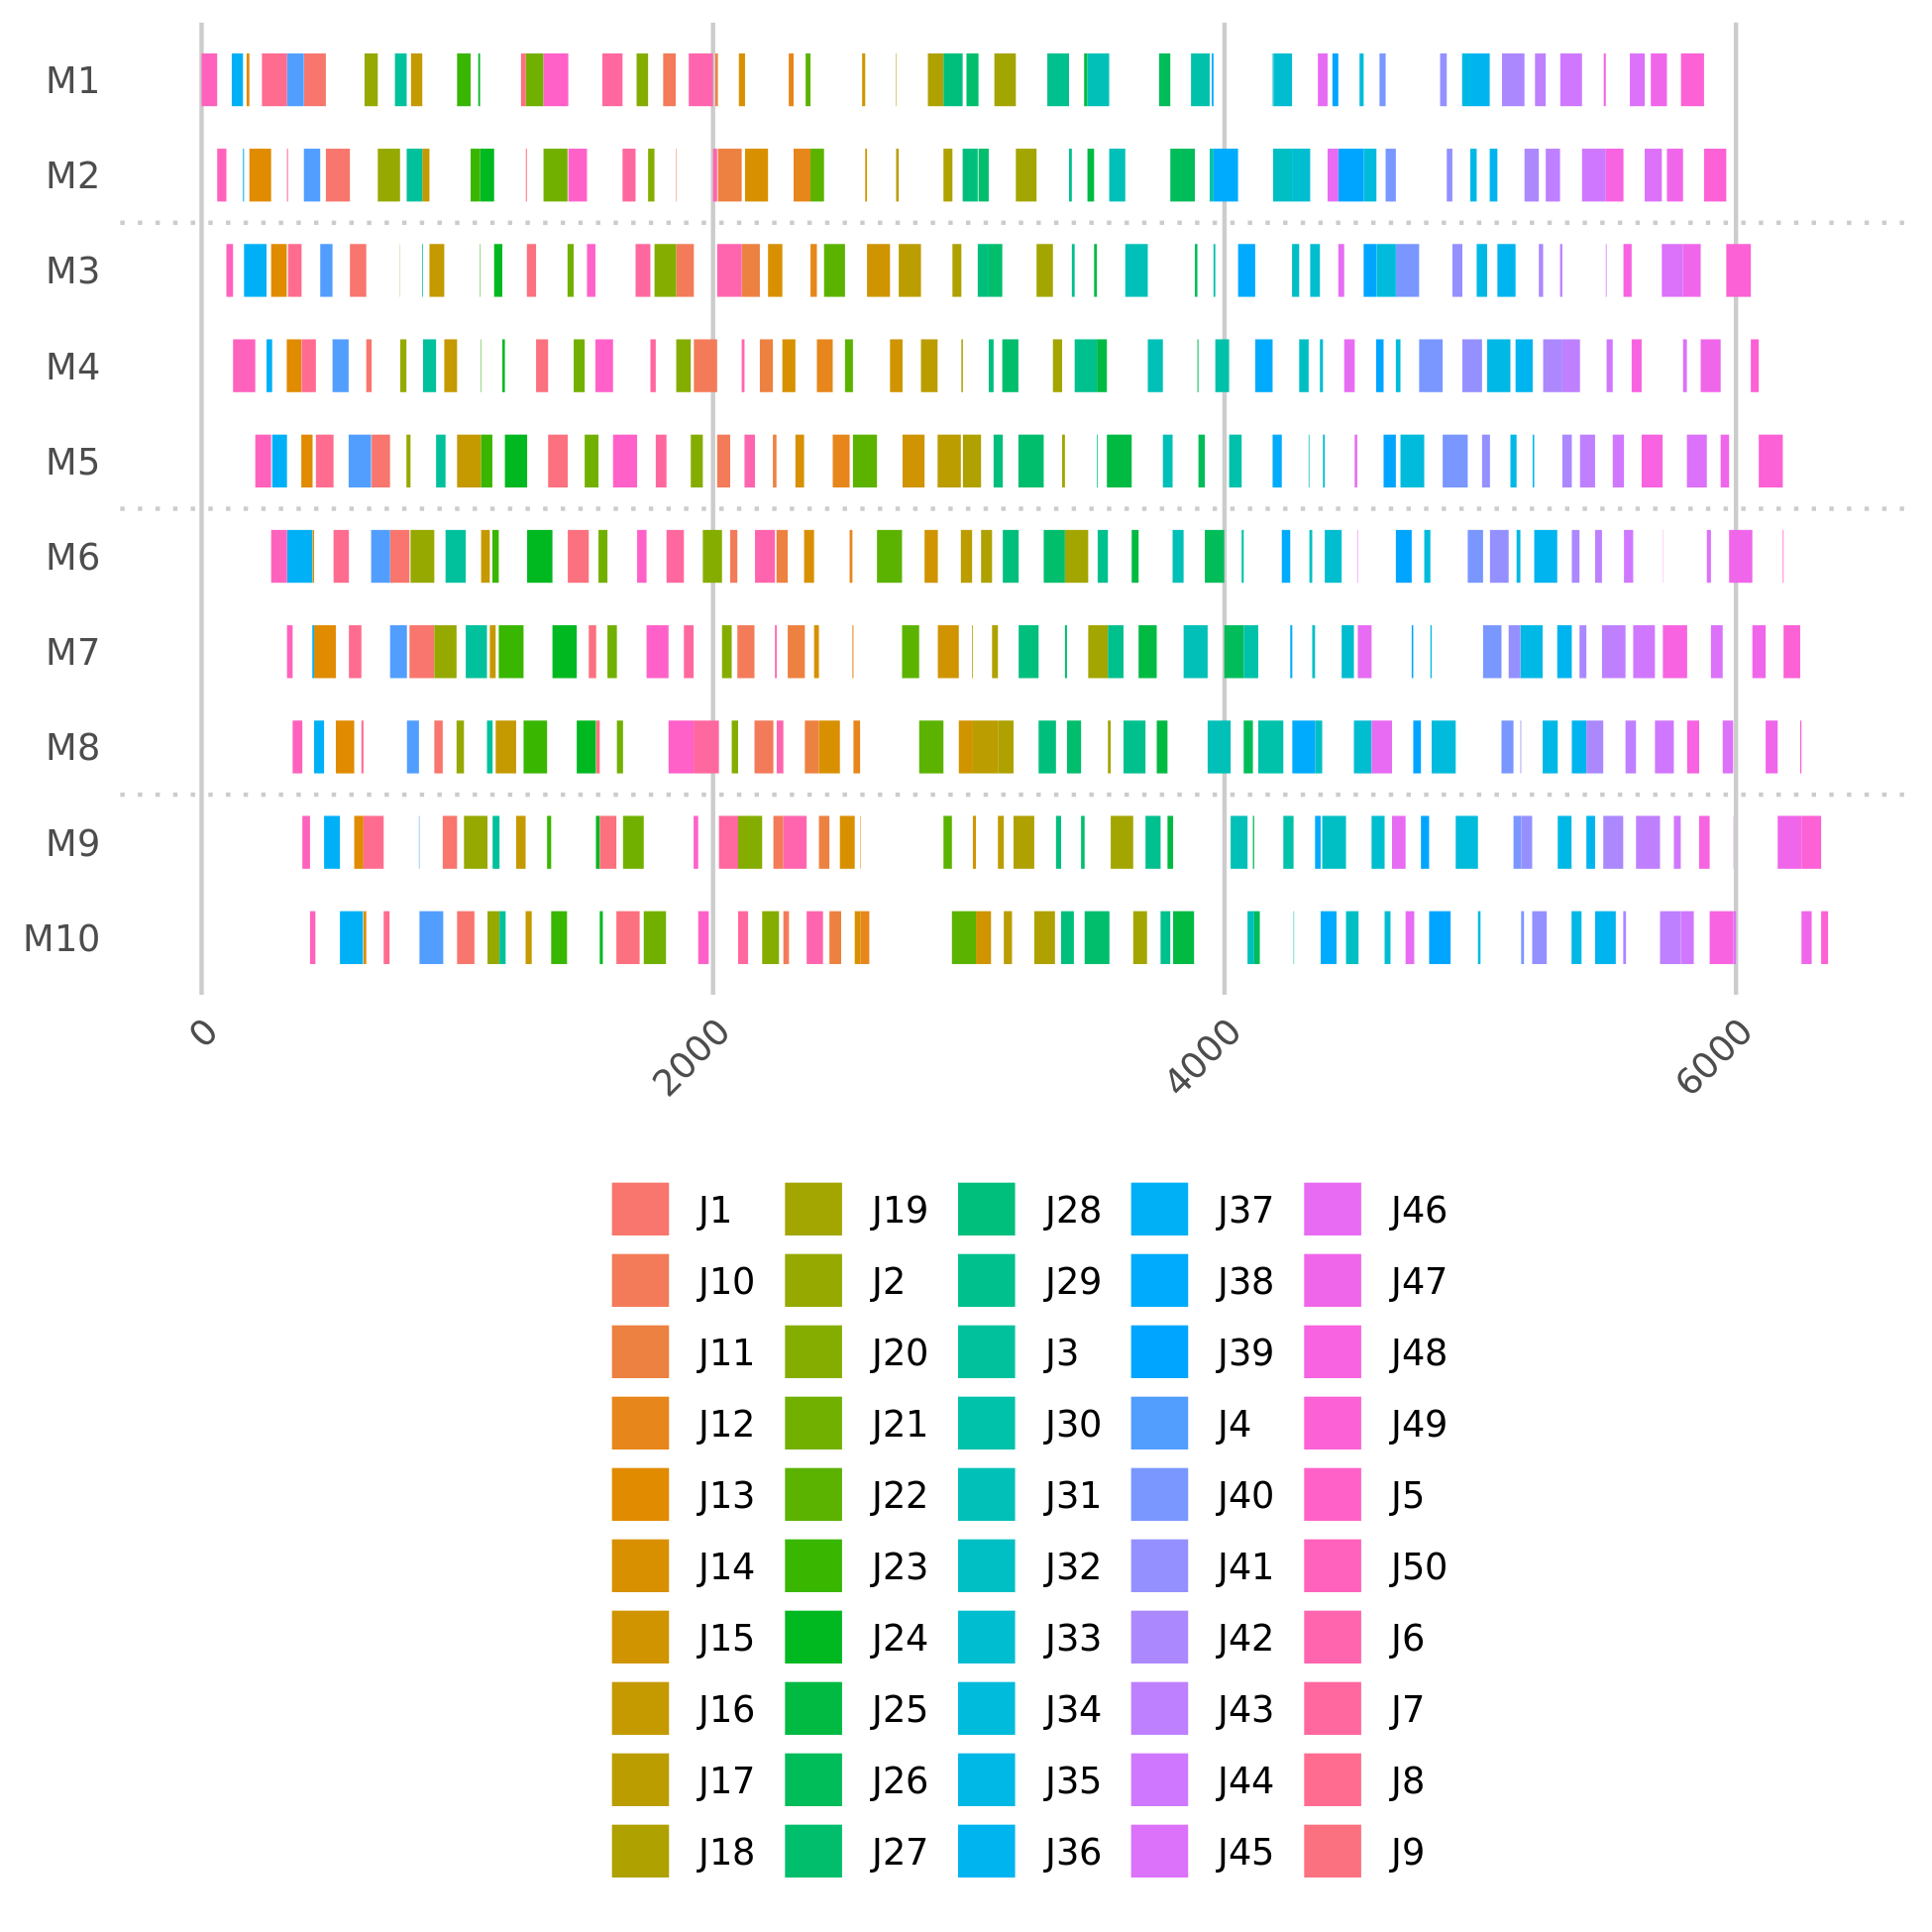
\includegraphics[width=\linewidth]{10_50_GC_3.png}
				\captionof{figure}{Gantt Chart for file 41.txt}
				
				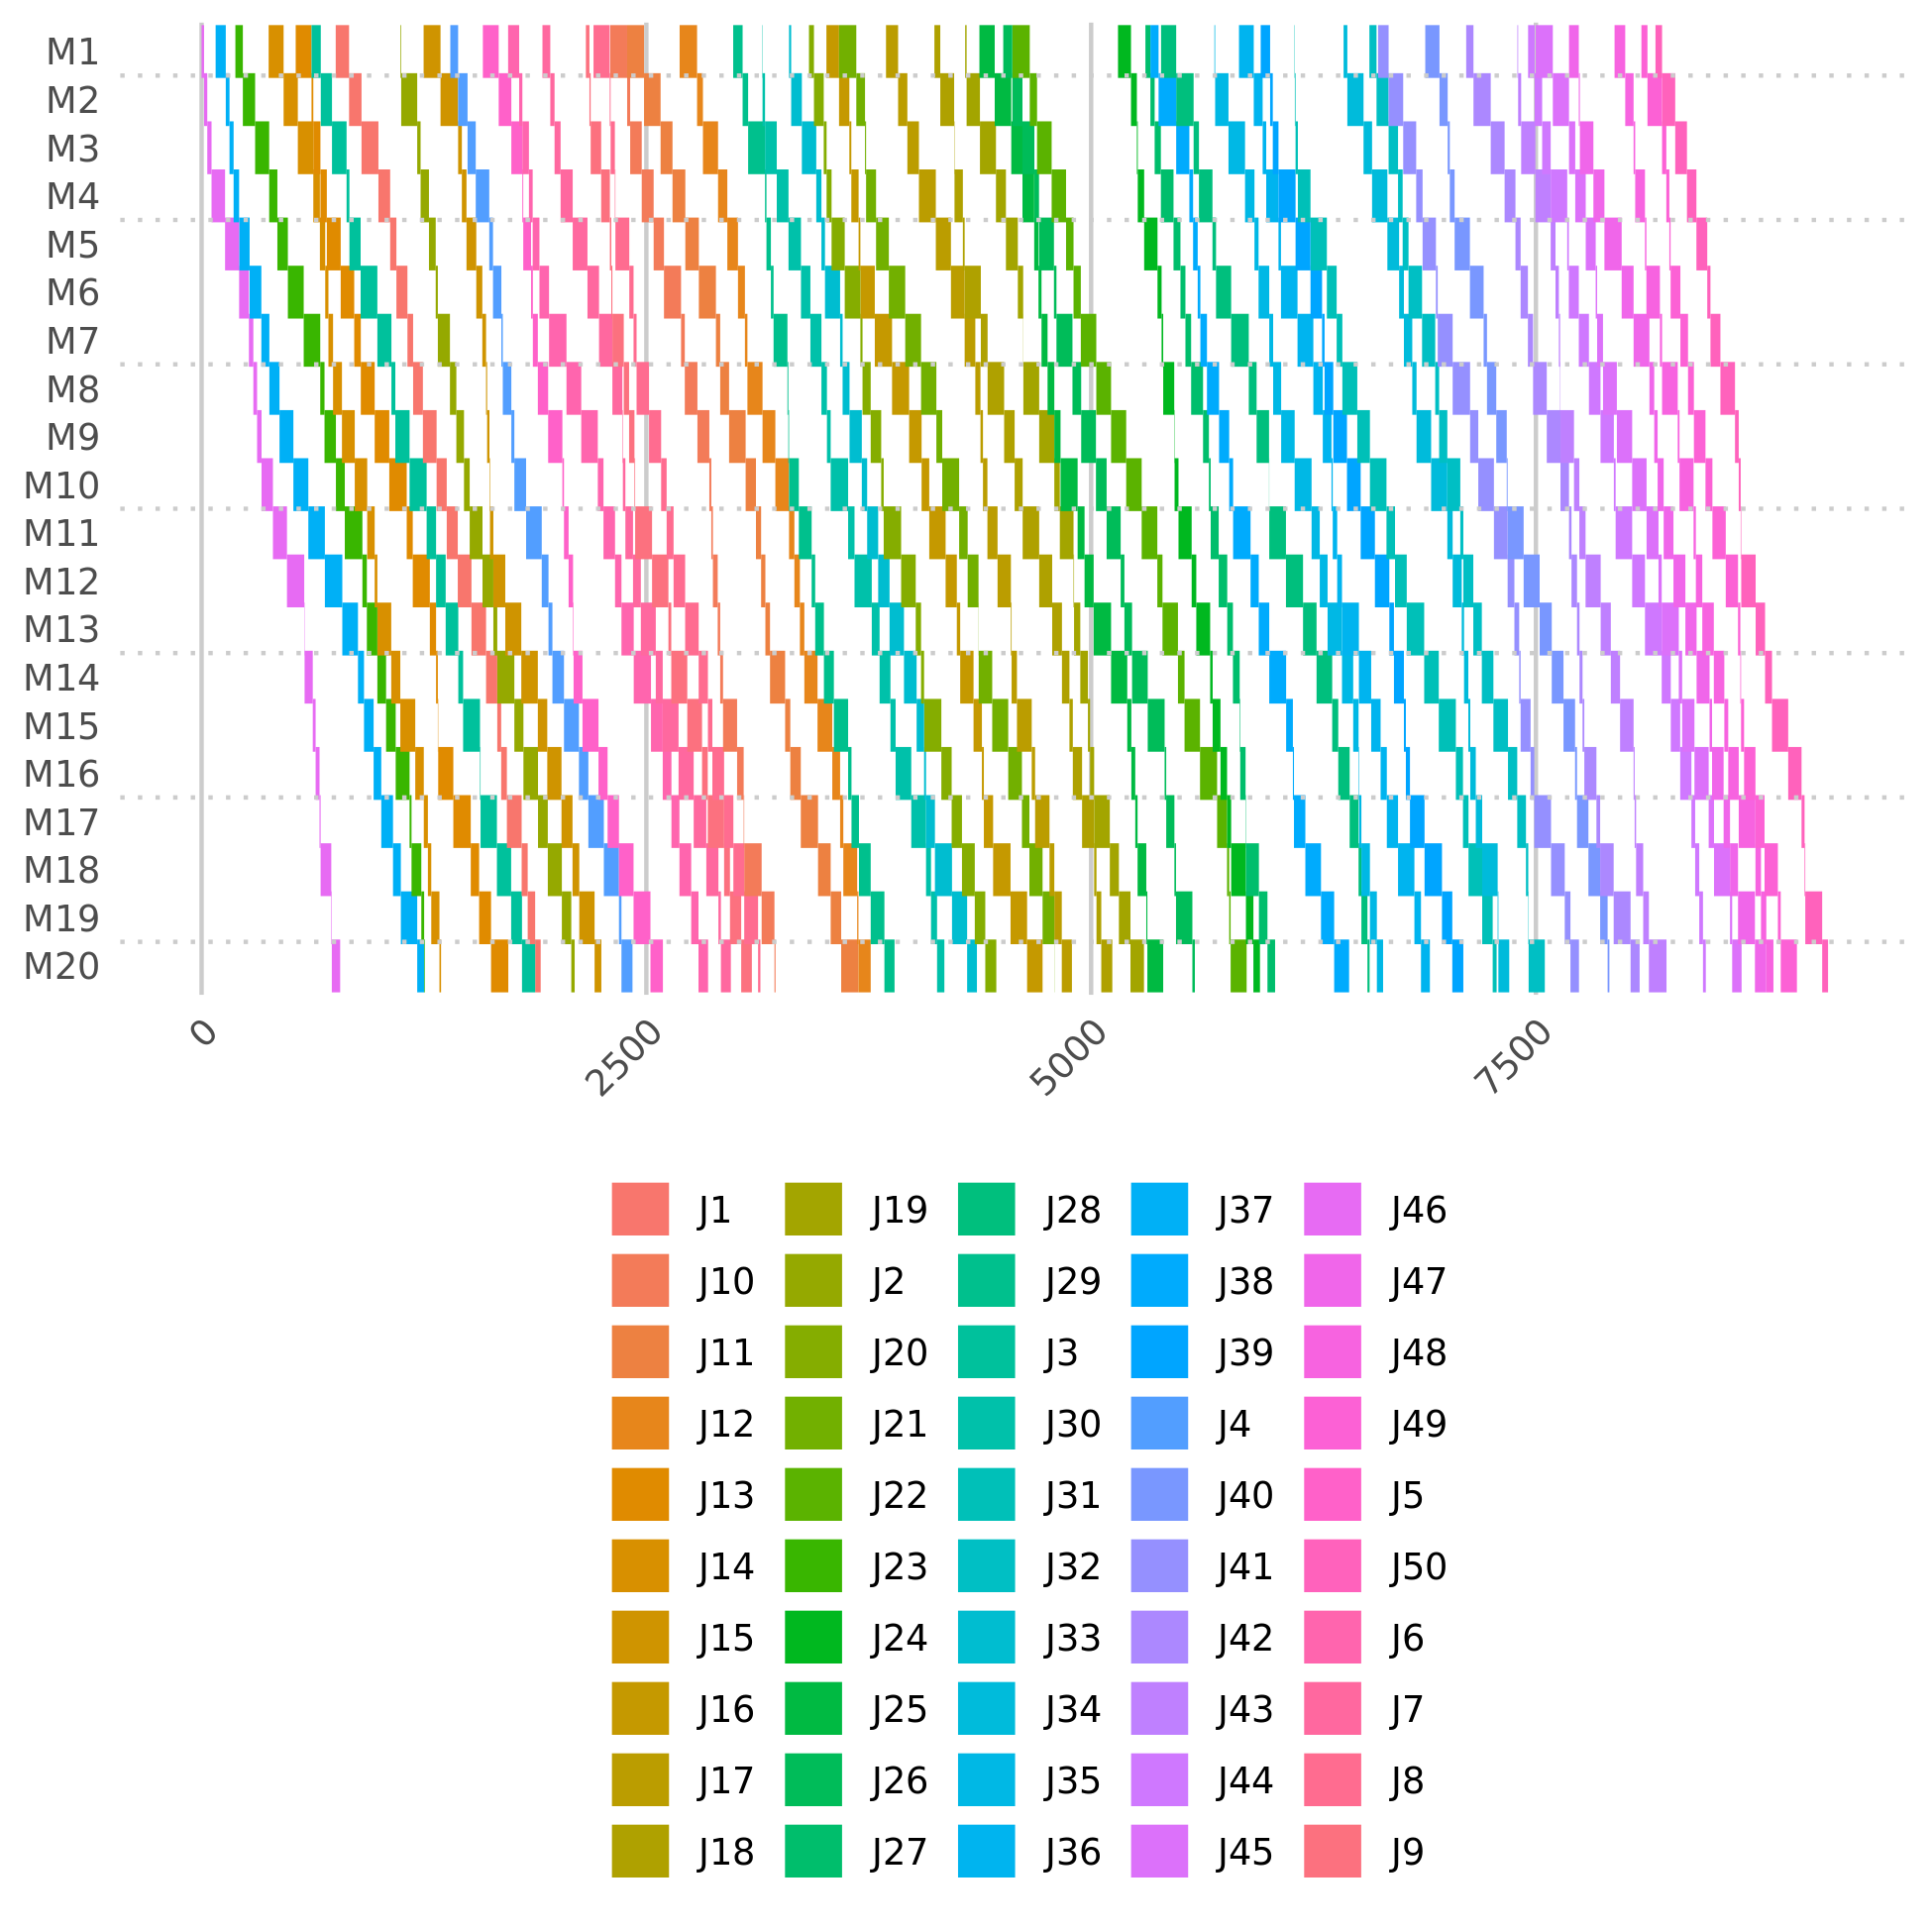
\includegraphics[width=\linewidth]{20_50_GC_3.png}
				\captionof{figure}{Gantt Chart for file 51.txt}
				
				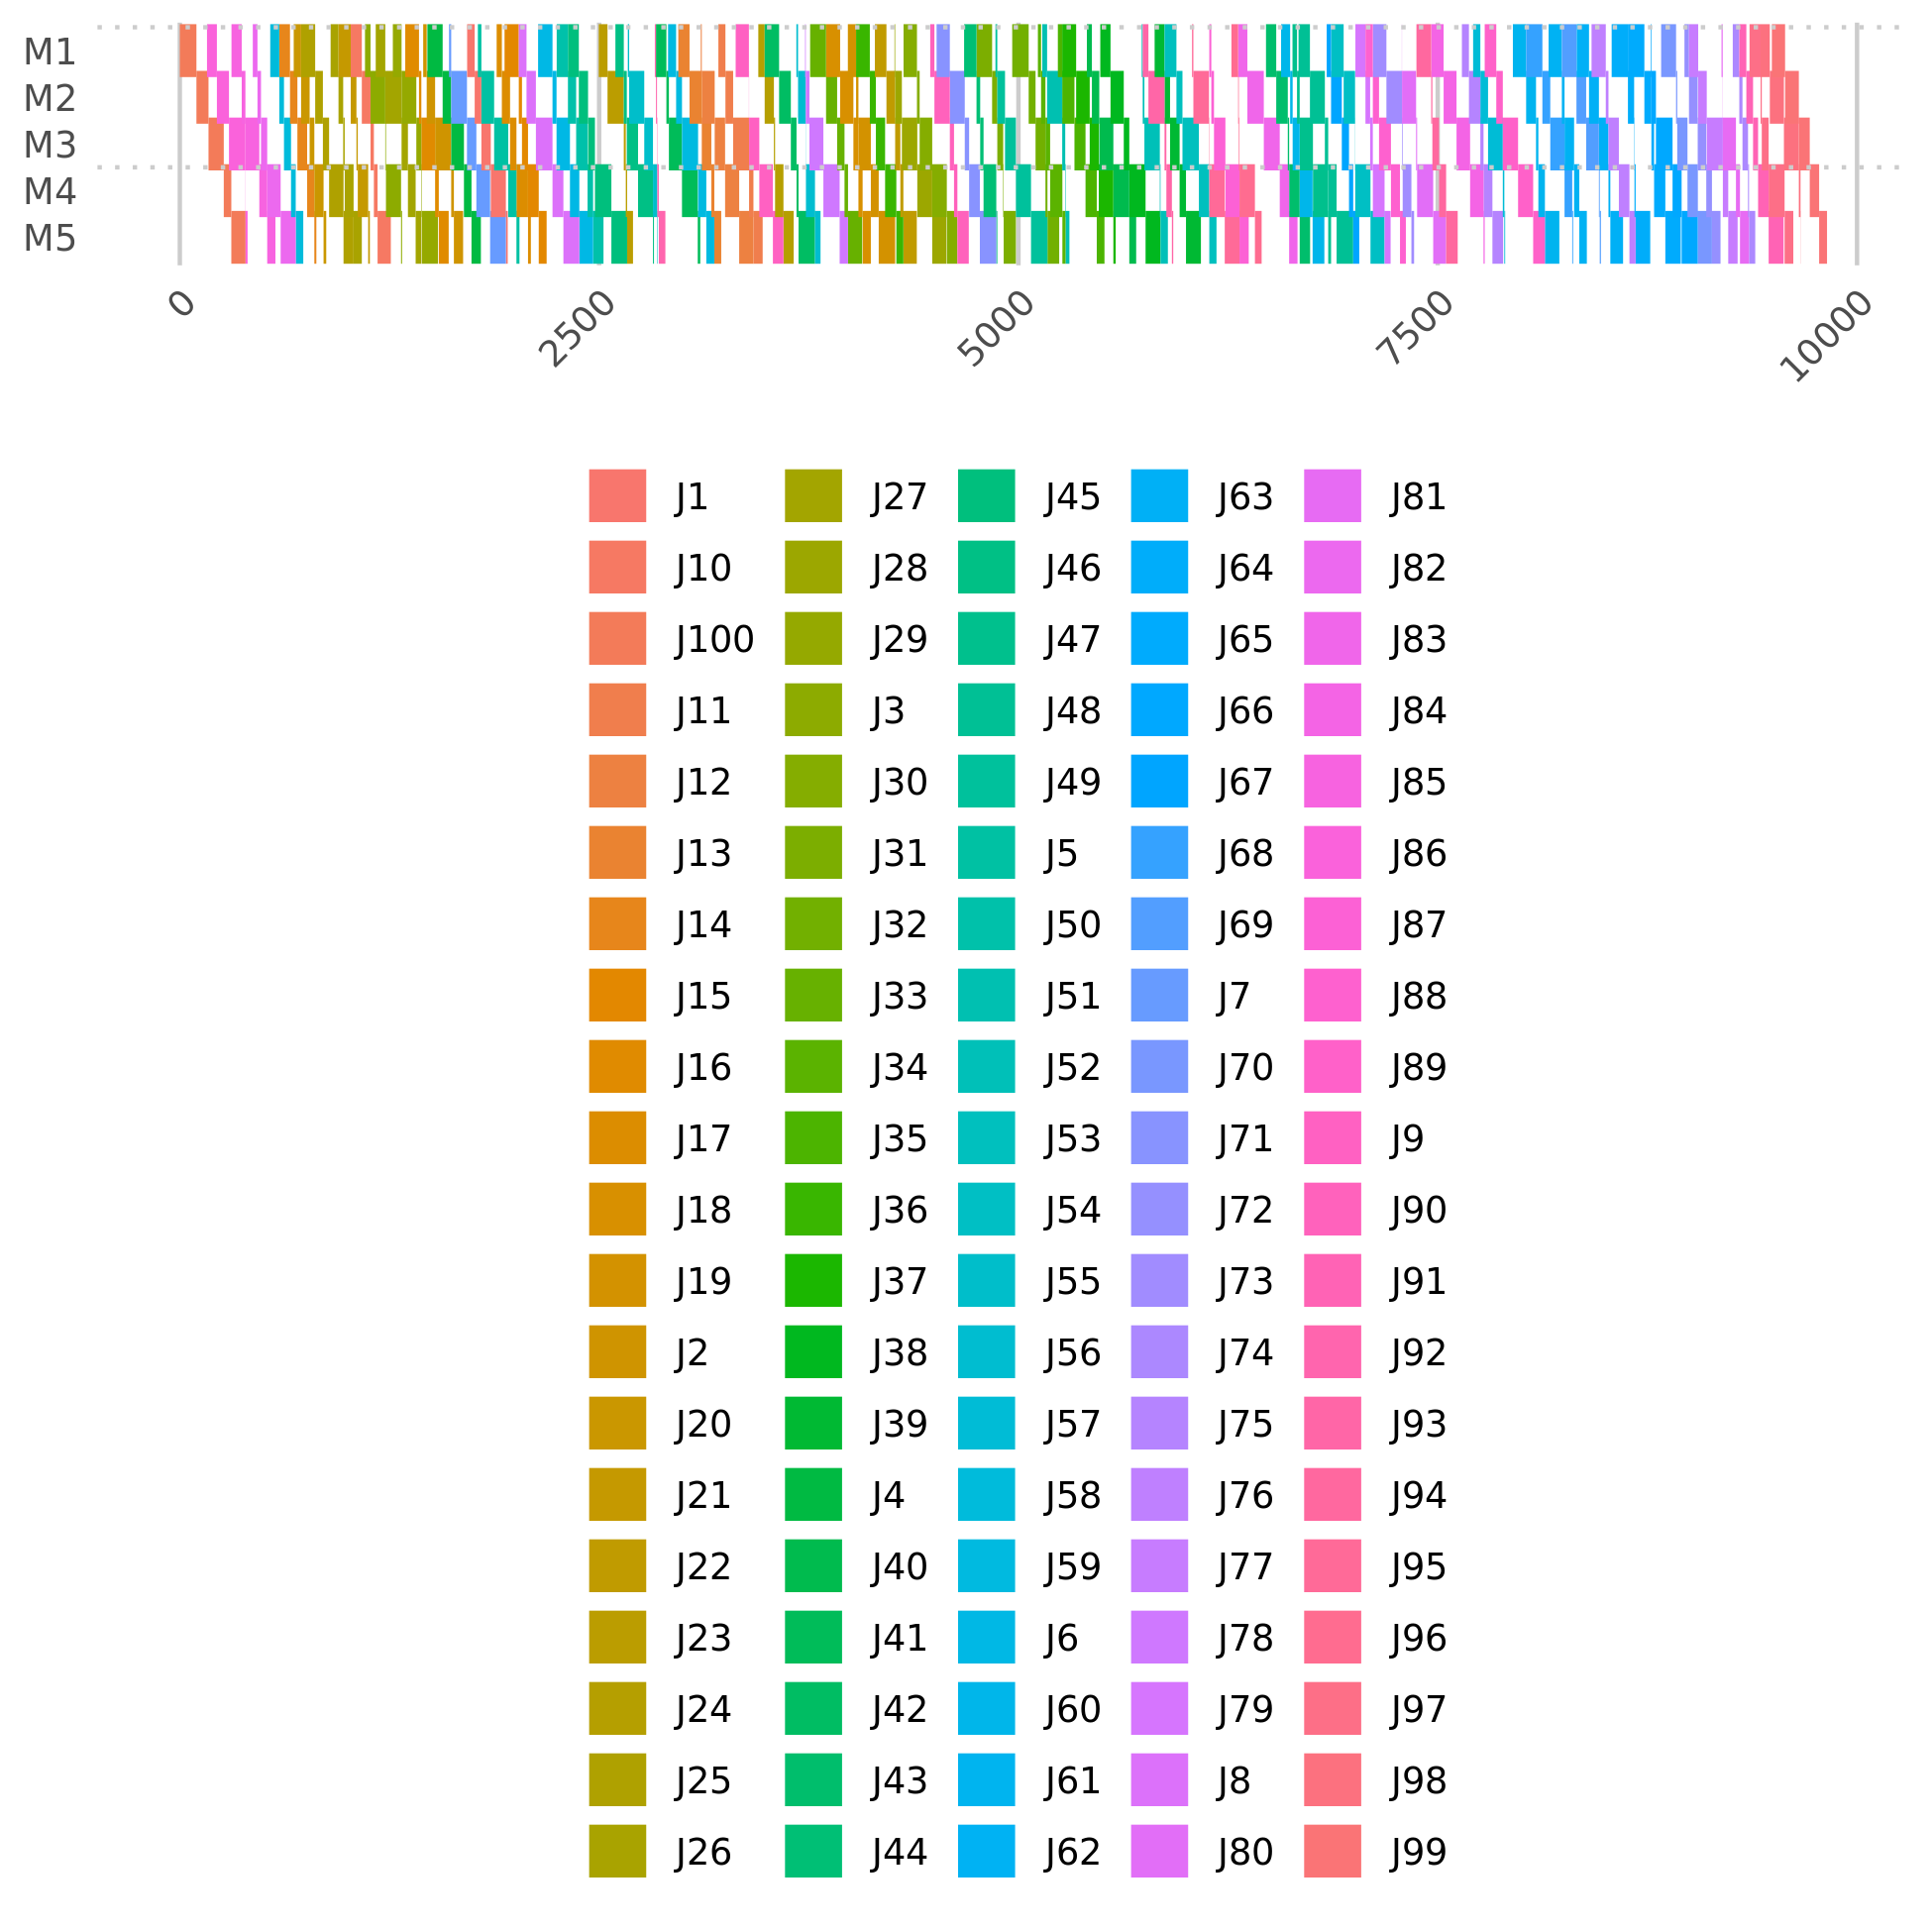
\includegraphics[width=\linewidth]{5_100_GC_3.png}
				\captionof{figure}{Gantt Chart for file 61.txt}
				
				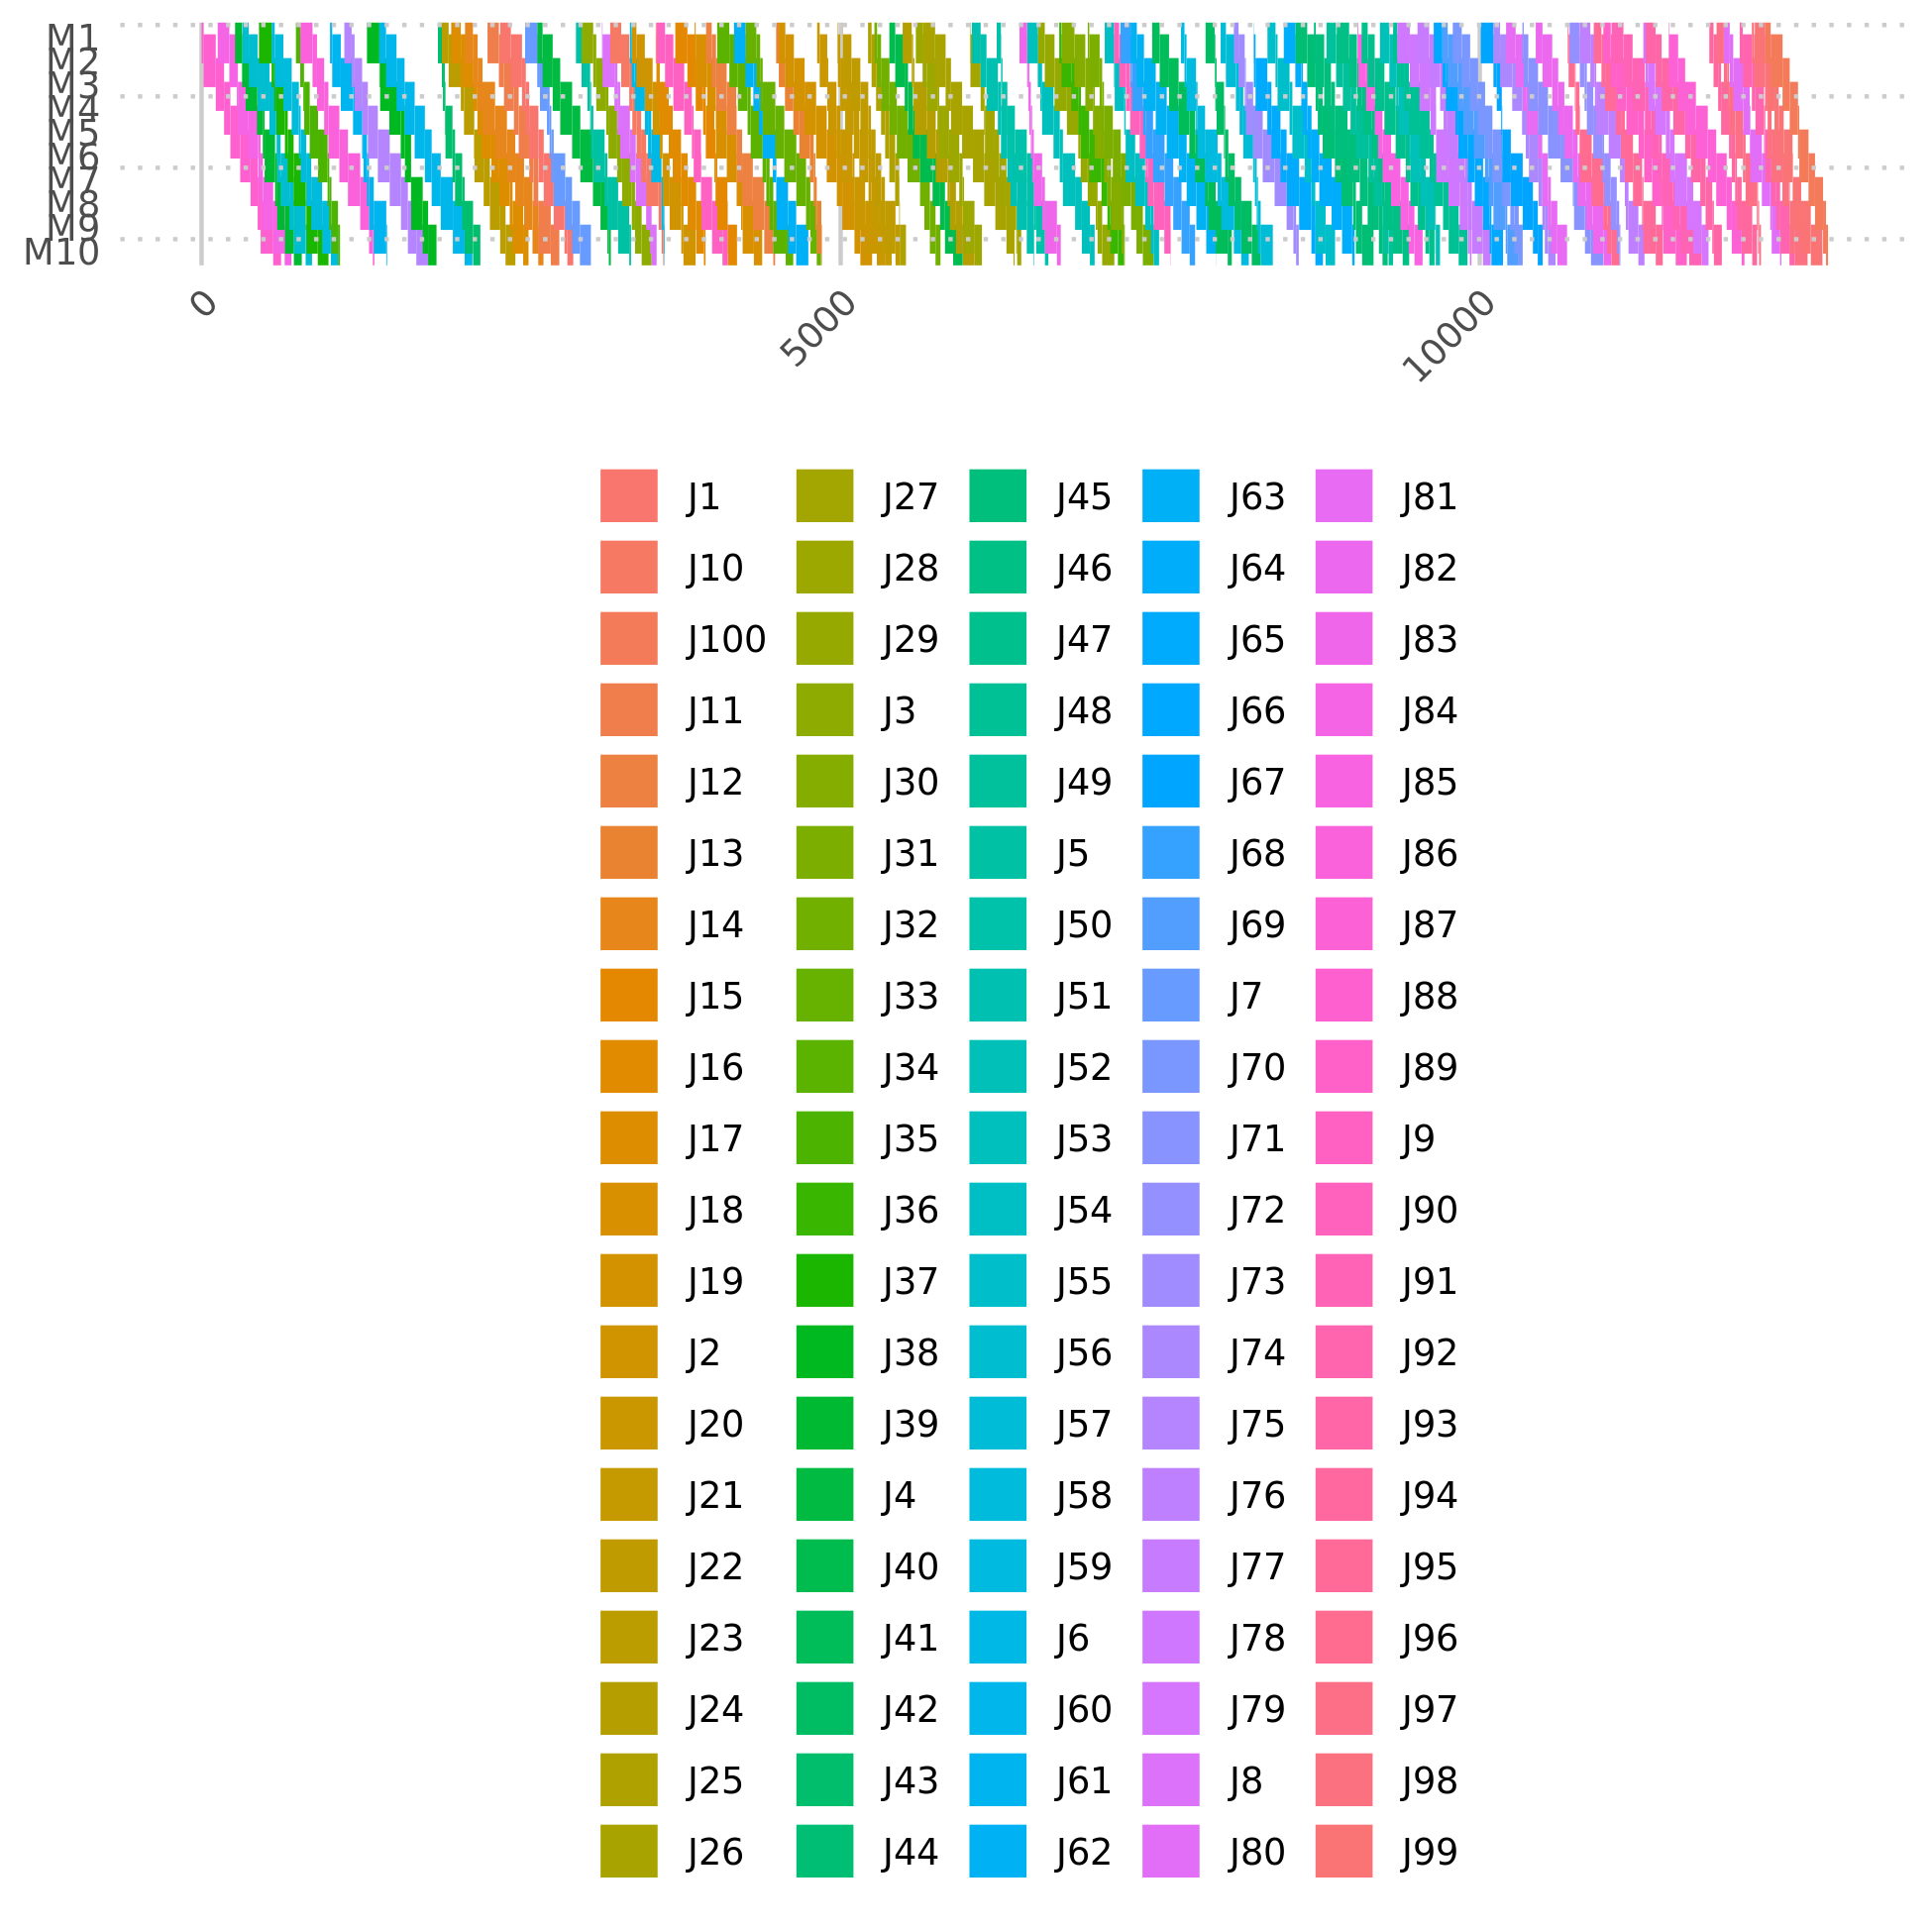
\includegraphics[width=\linewidth]{10_100_GC_3.png}
				\captionof{figure}{Gantt Chart for file 71.txt}
				
				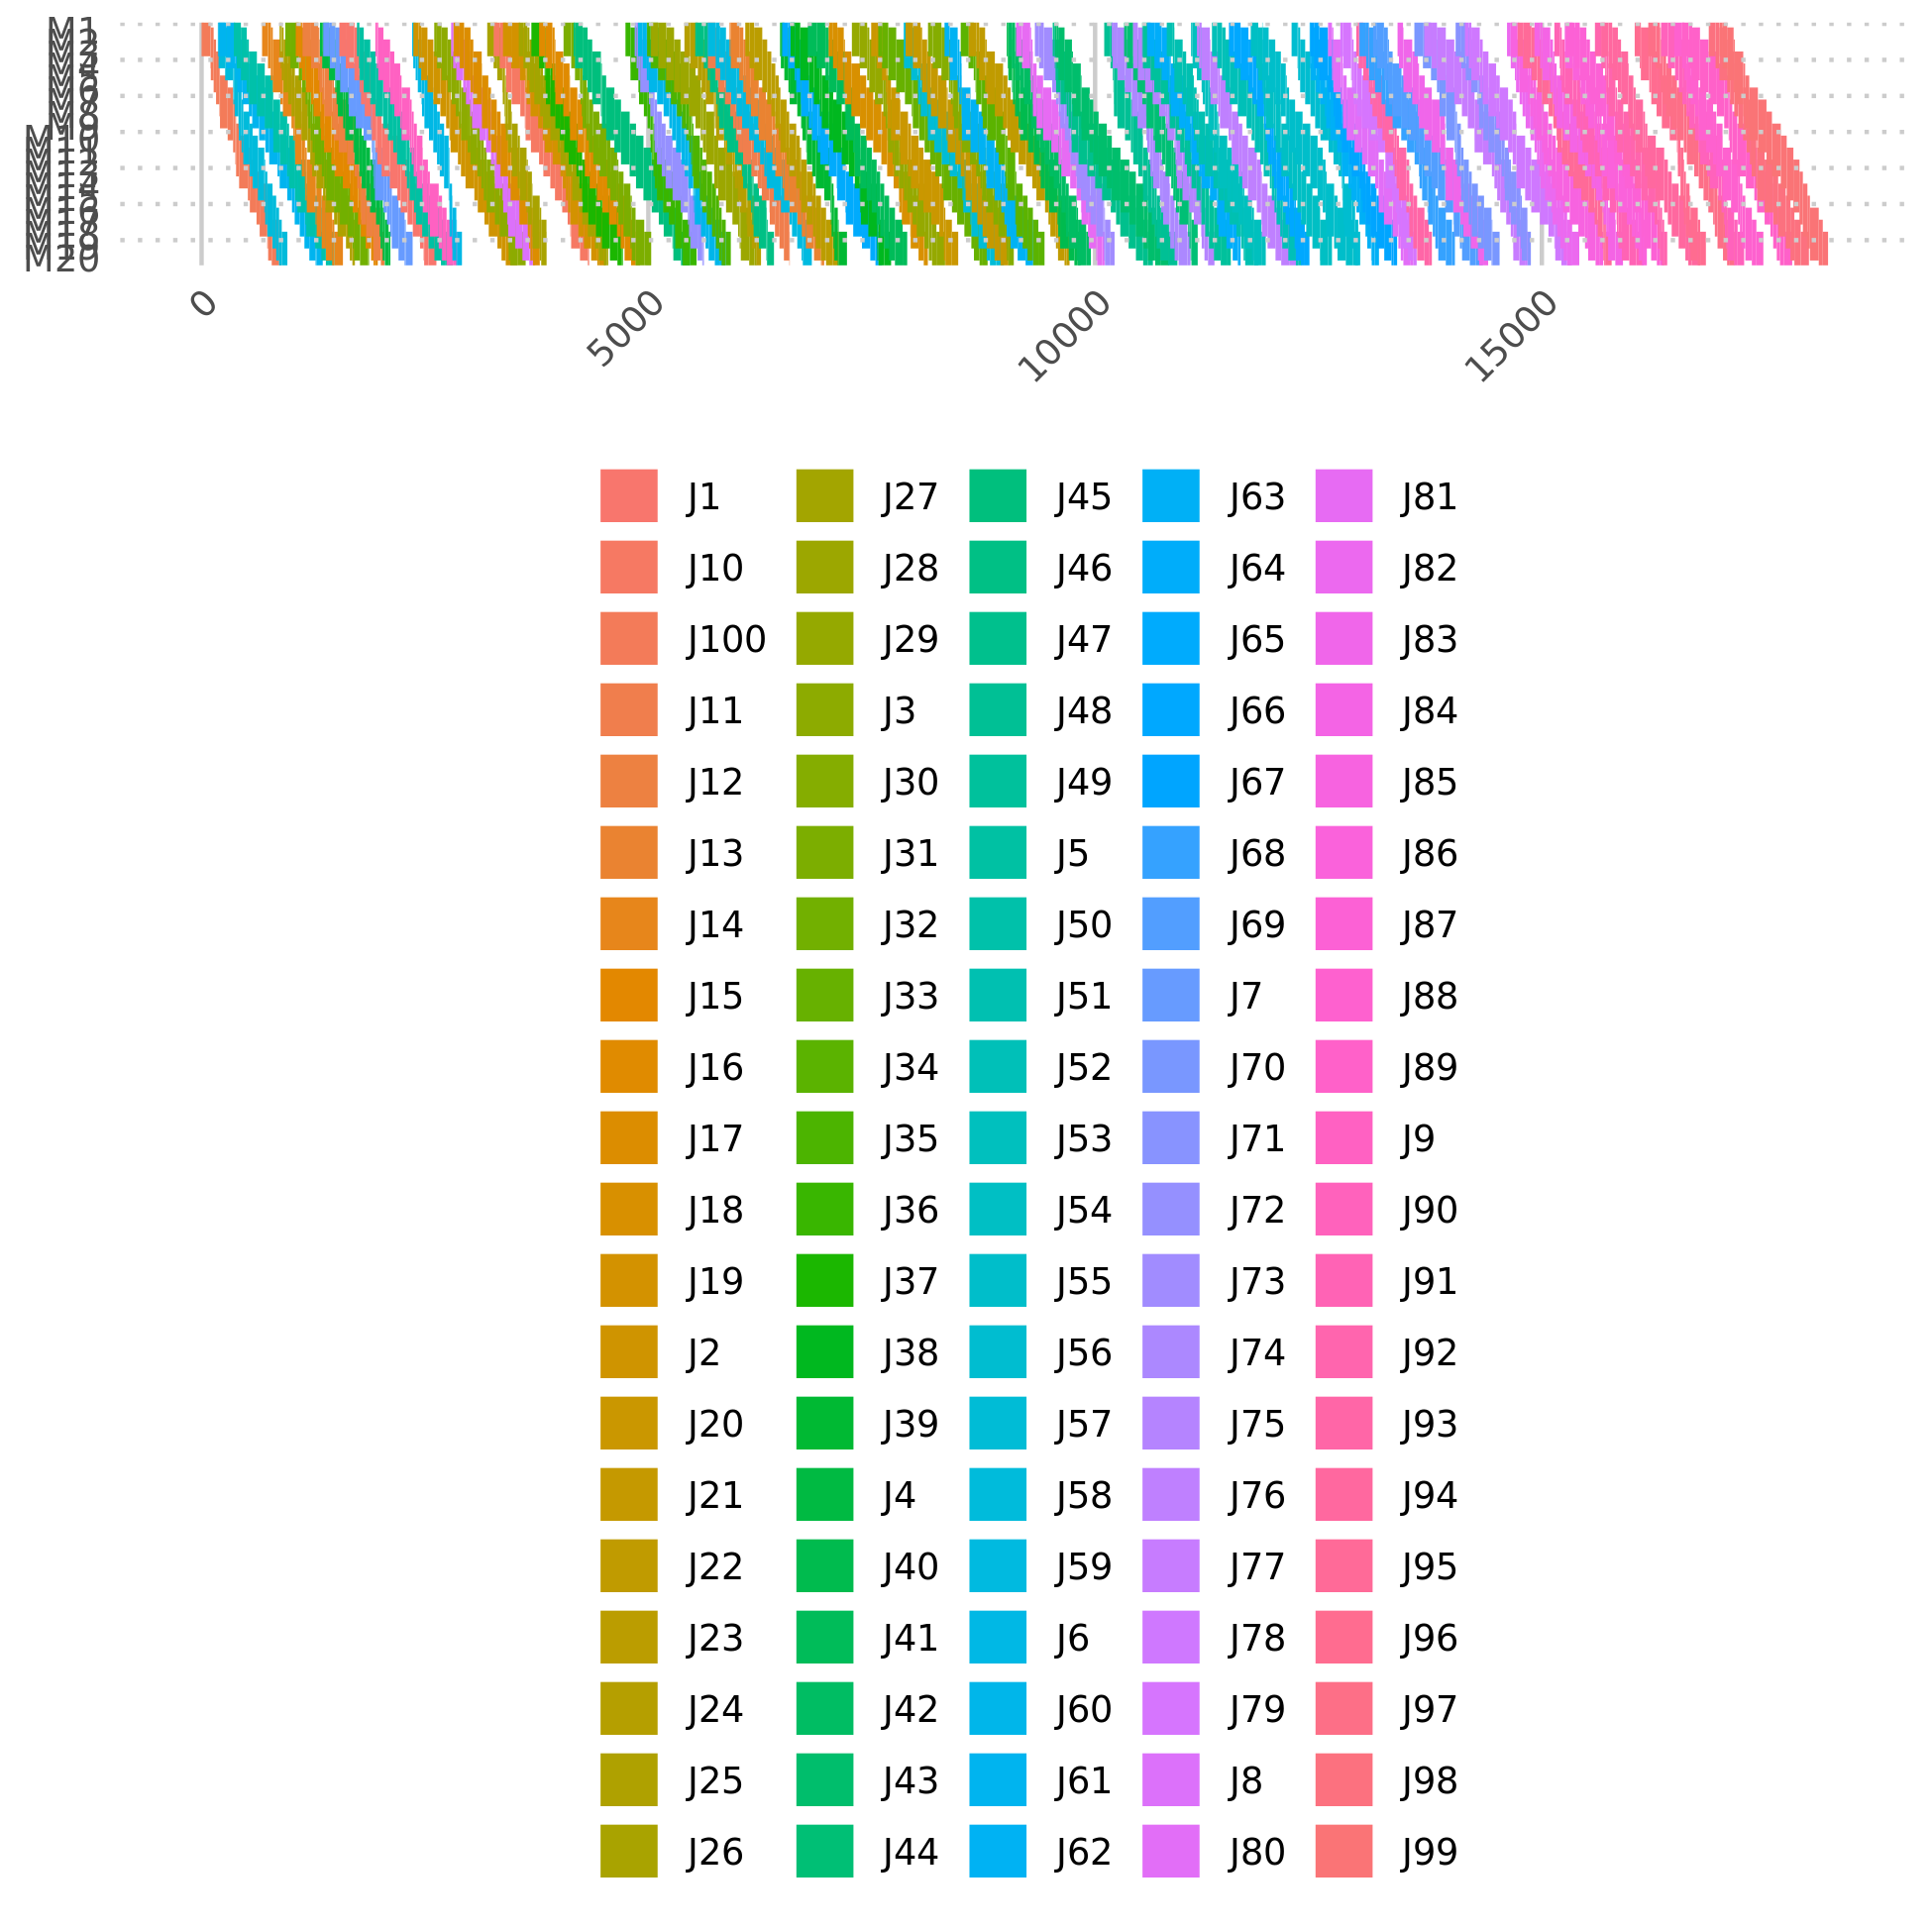
\includegraphics[width=\linewidth]{20_100_GC_3.png}
				\captionof{figure}{Gantt Chart for file 81.txt}
				
				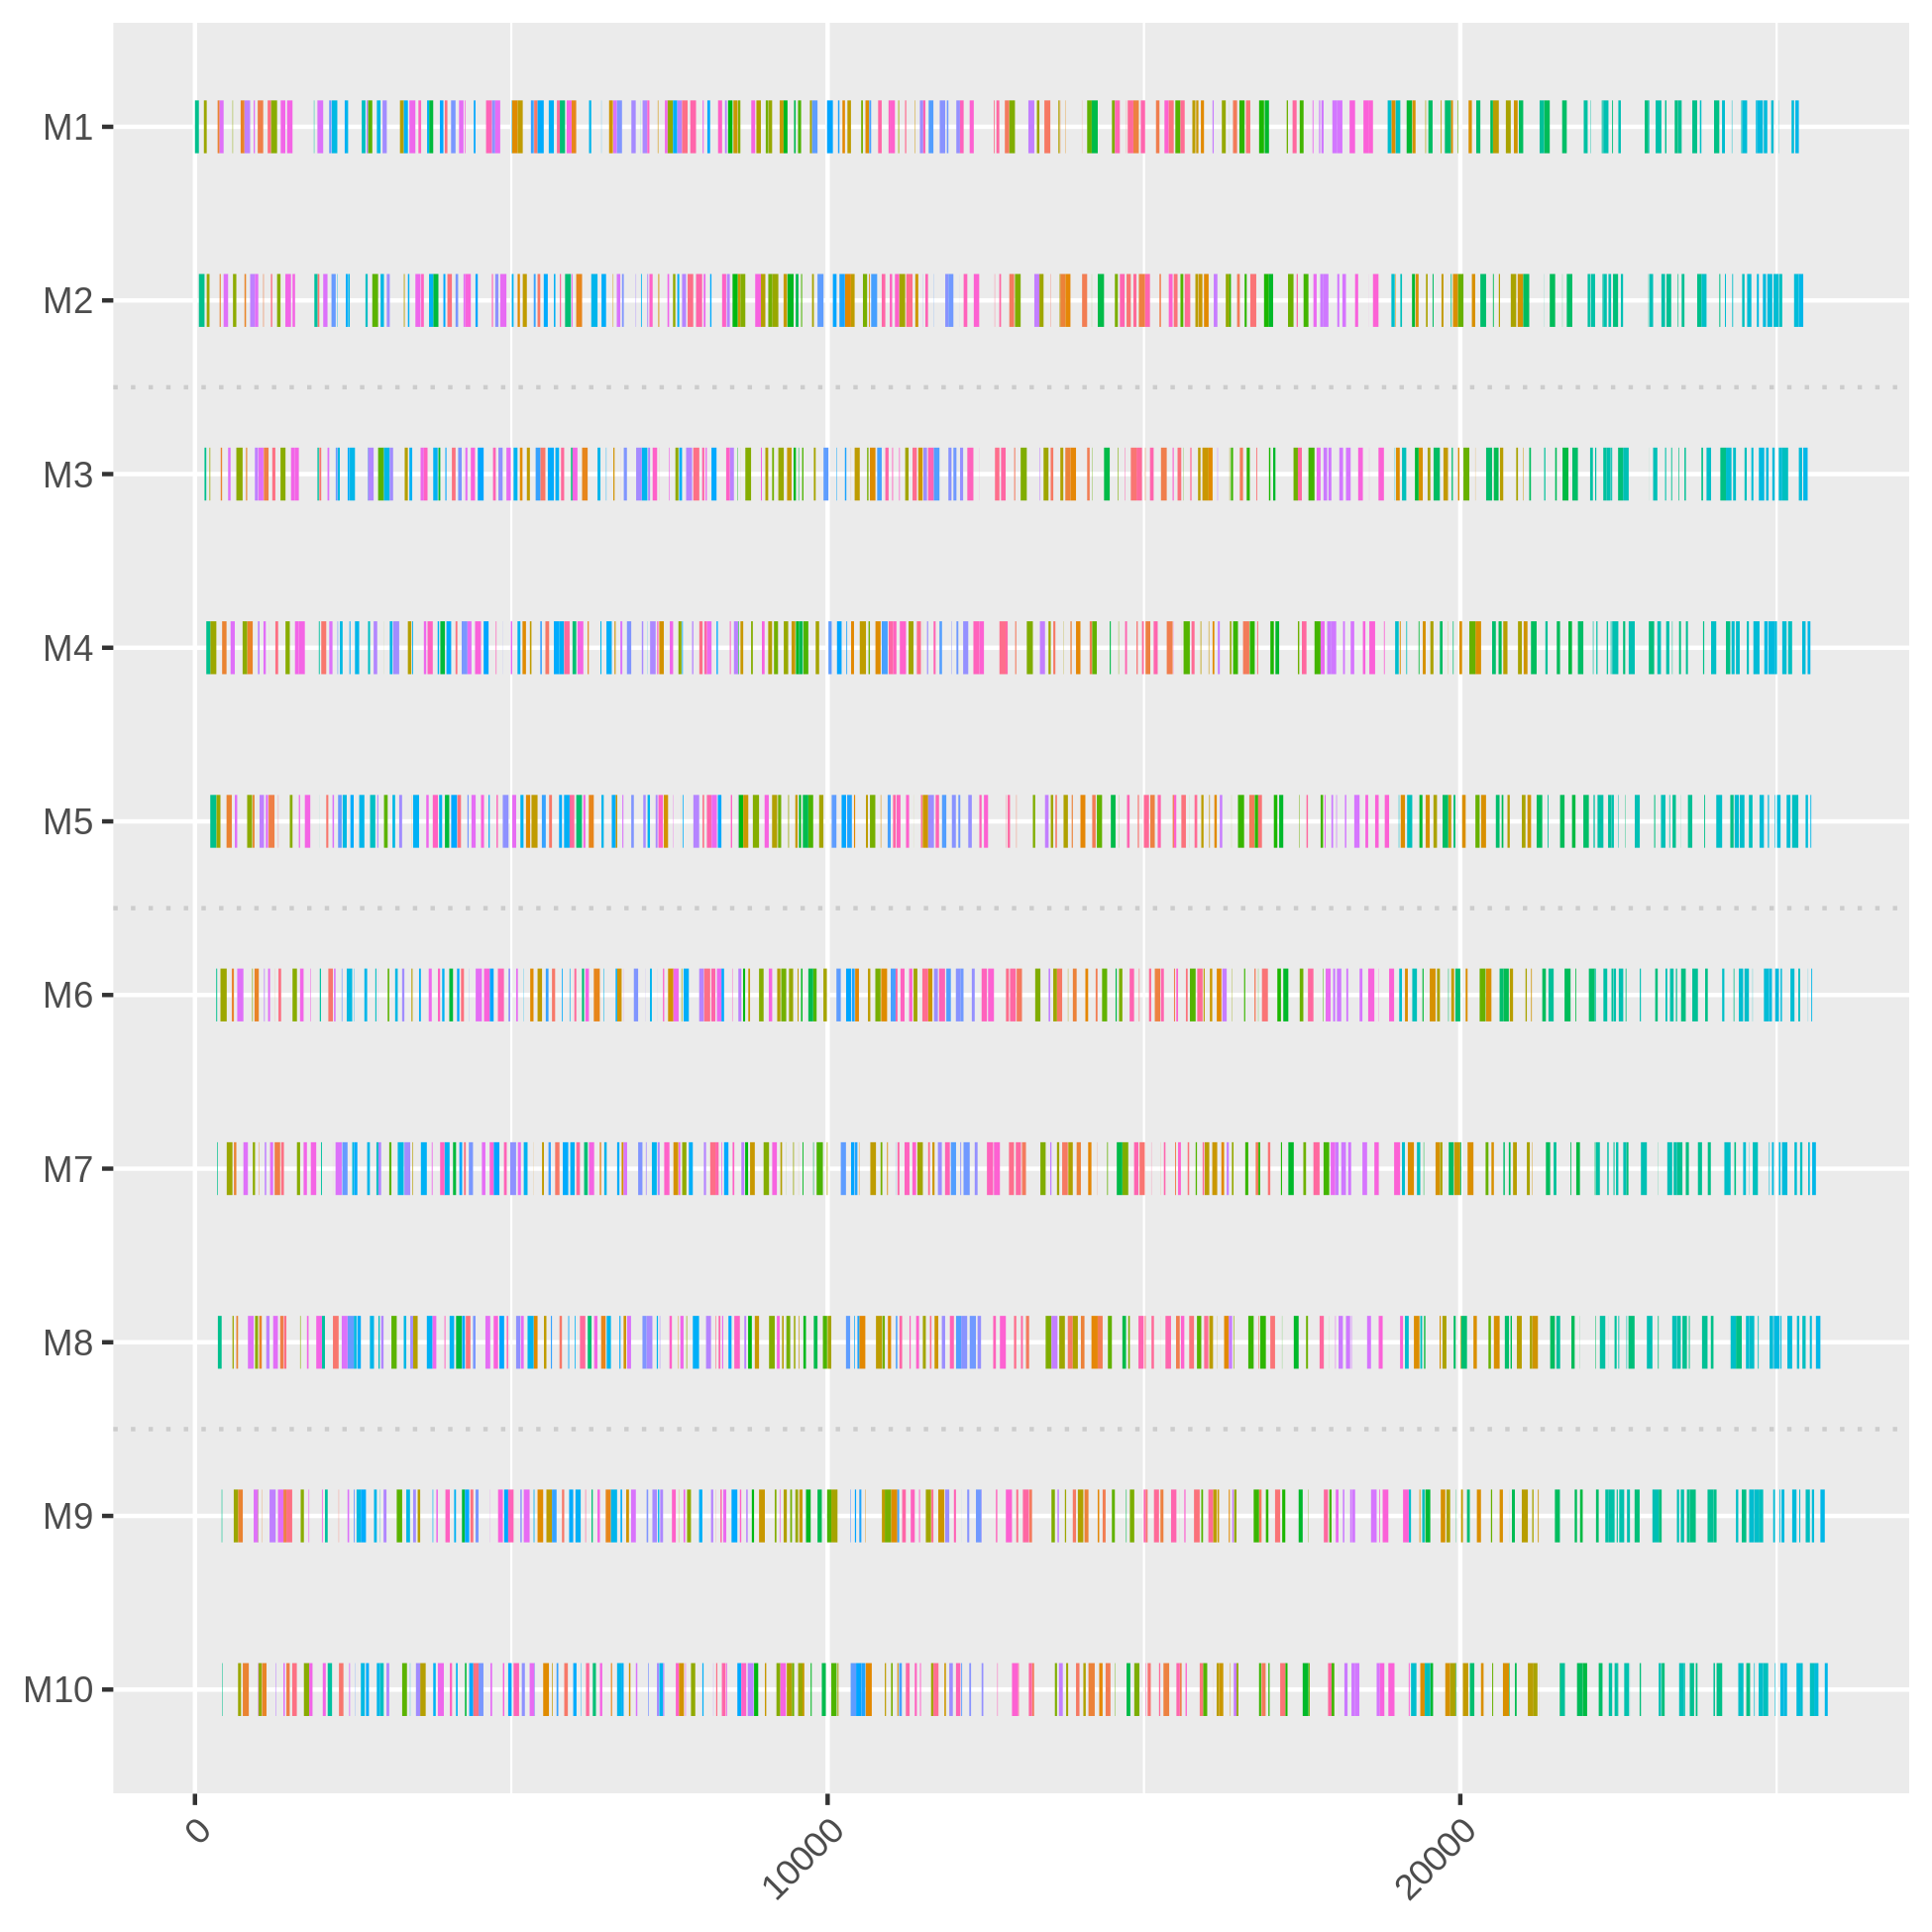
\includegraphics[width=\linewidth]{10_200_GC_3.png}
				\captionof{figure}{Gantt Chart for file 91.txt}
				
				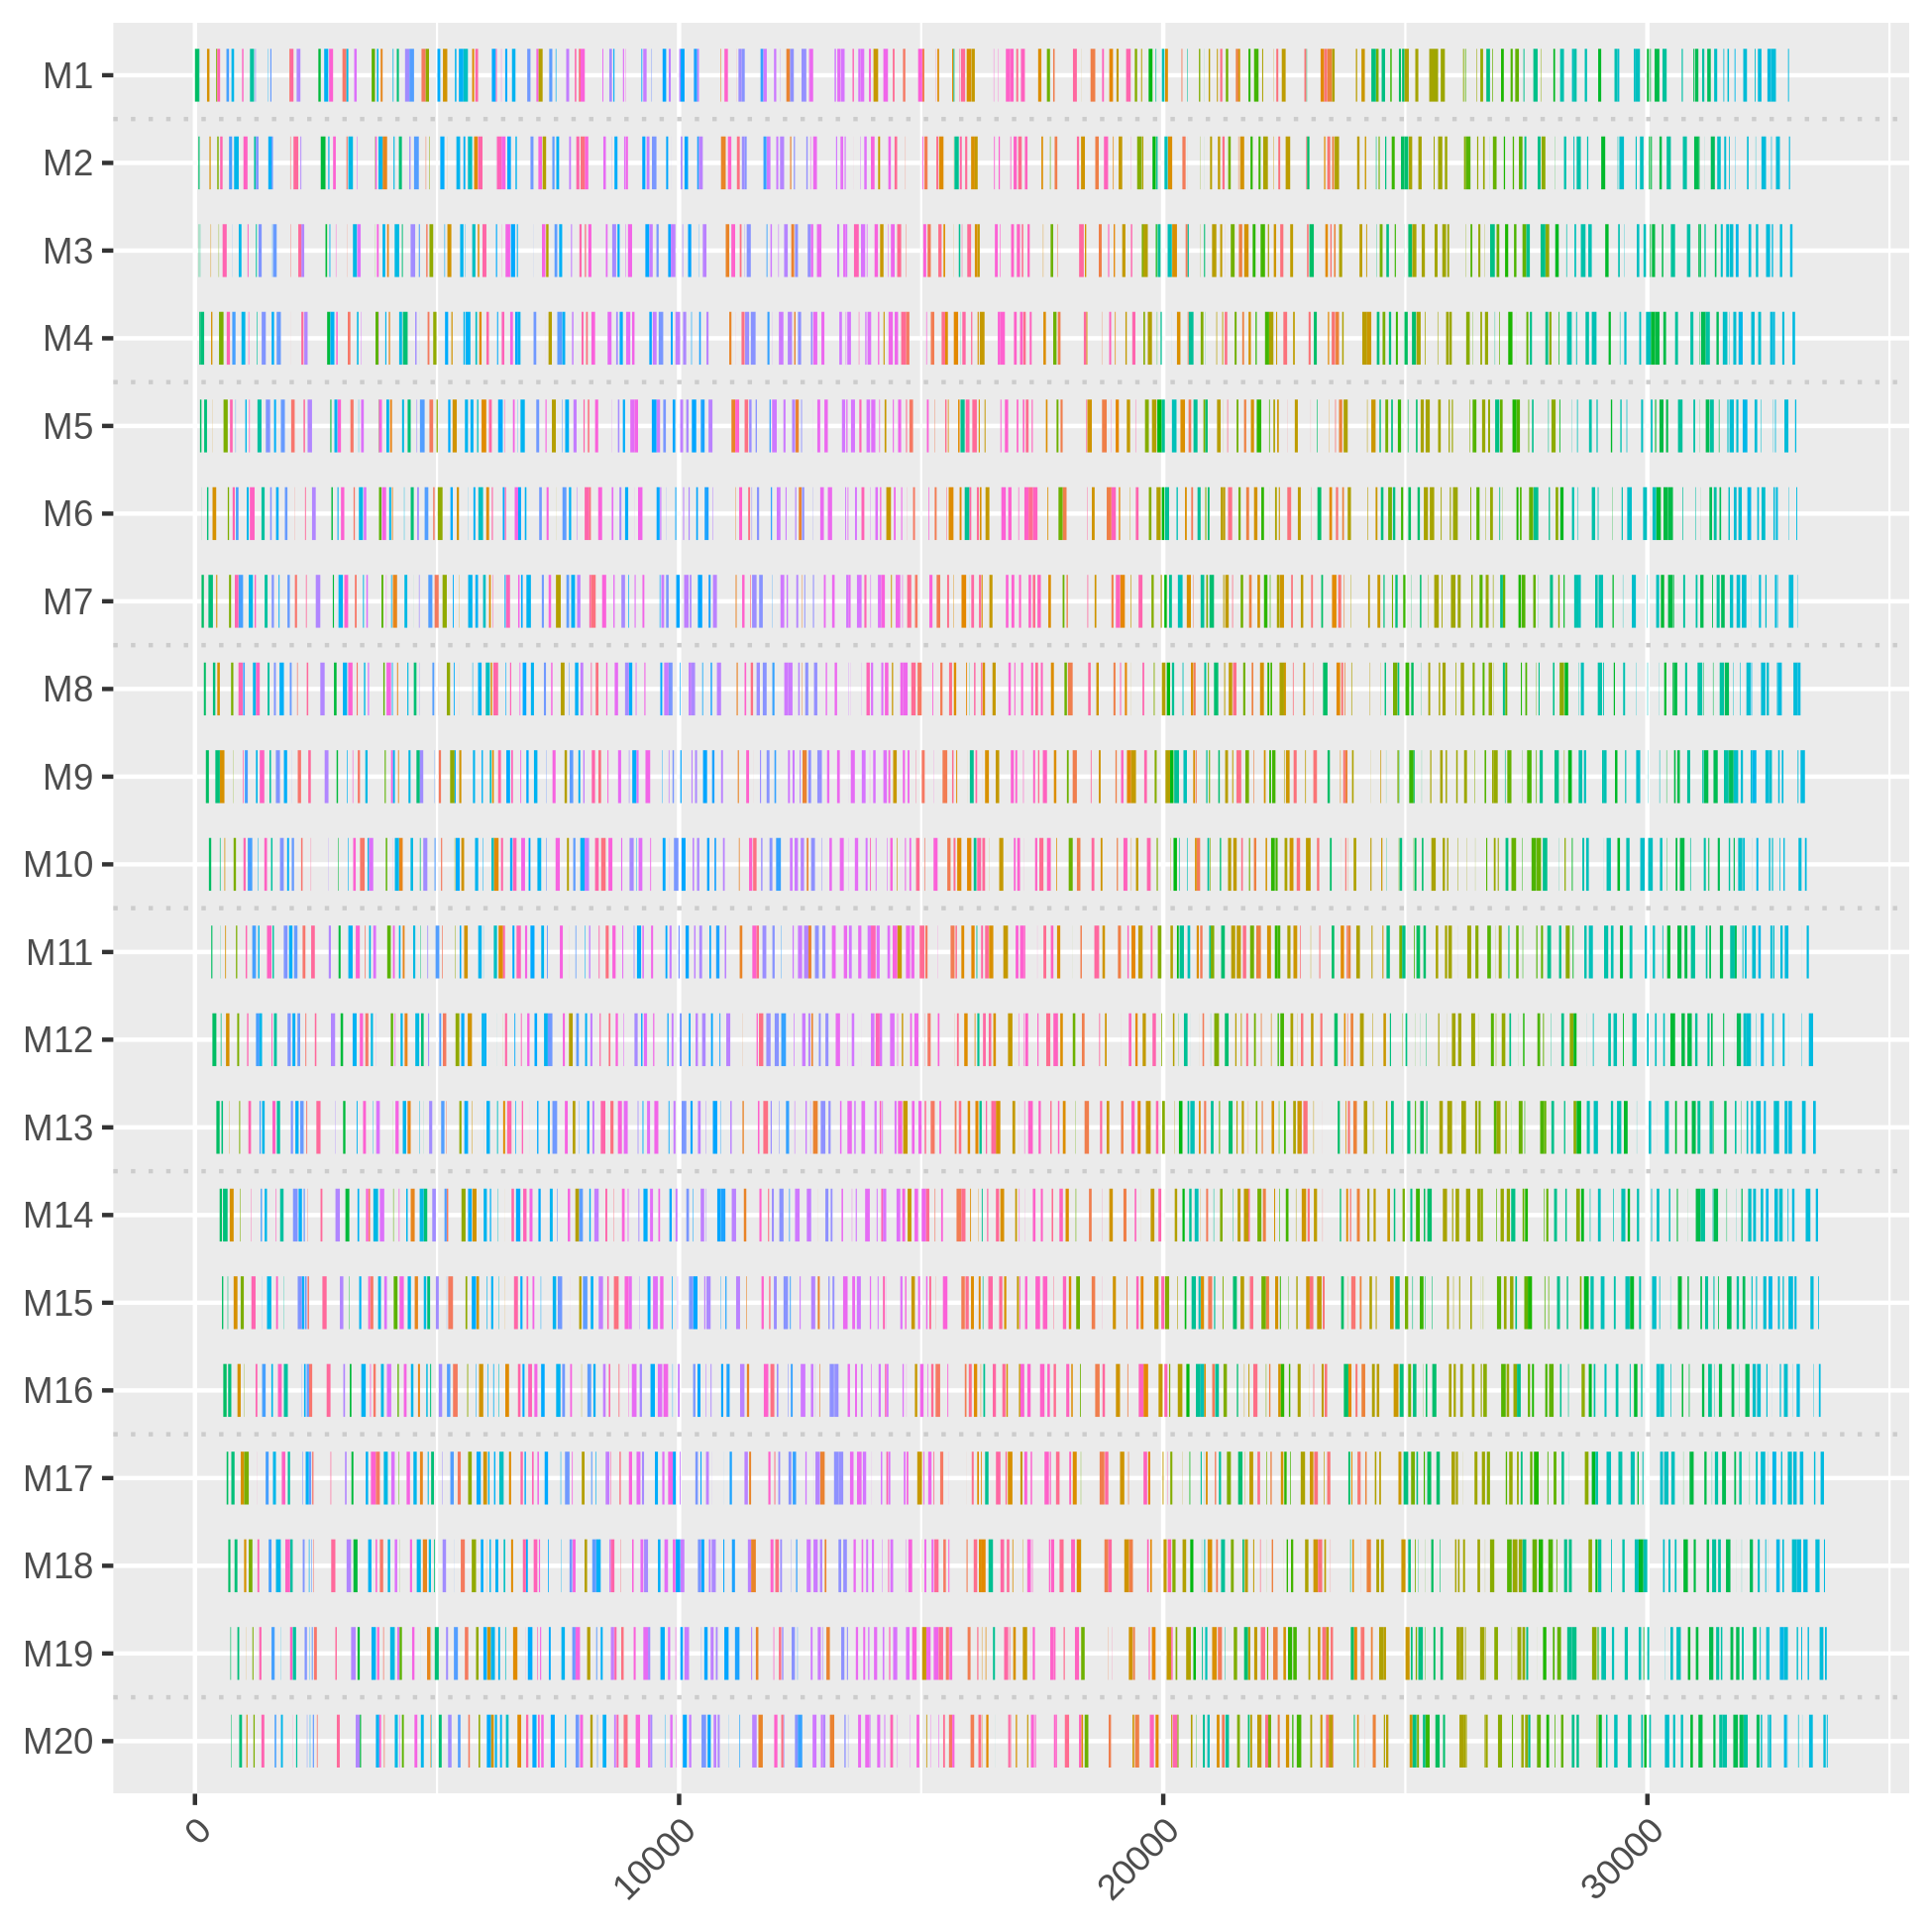
\includegraphics[width=\linewidth]{20_200_GC_3.png}
				\captionof{figure}{Gantt Chart for file 101.txt}
				
				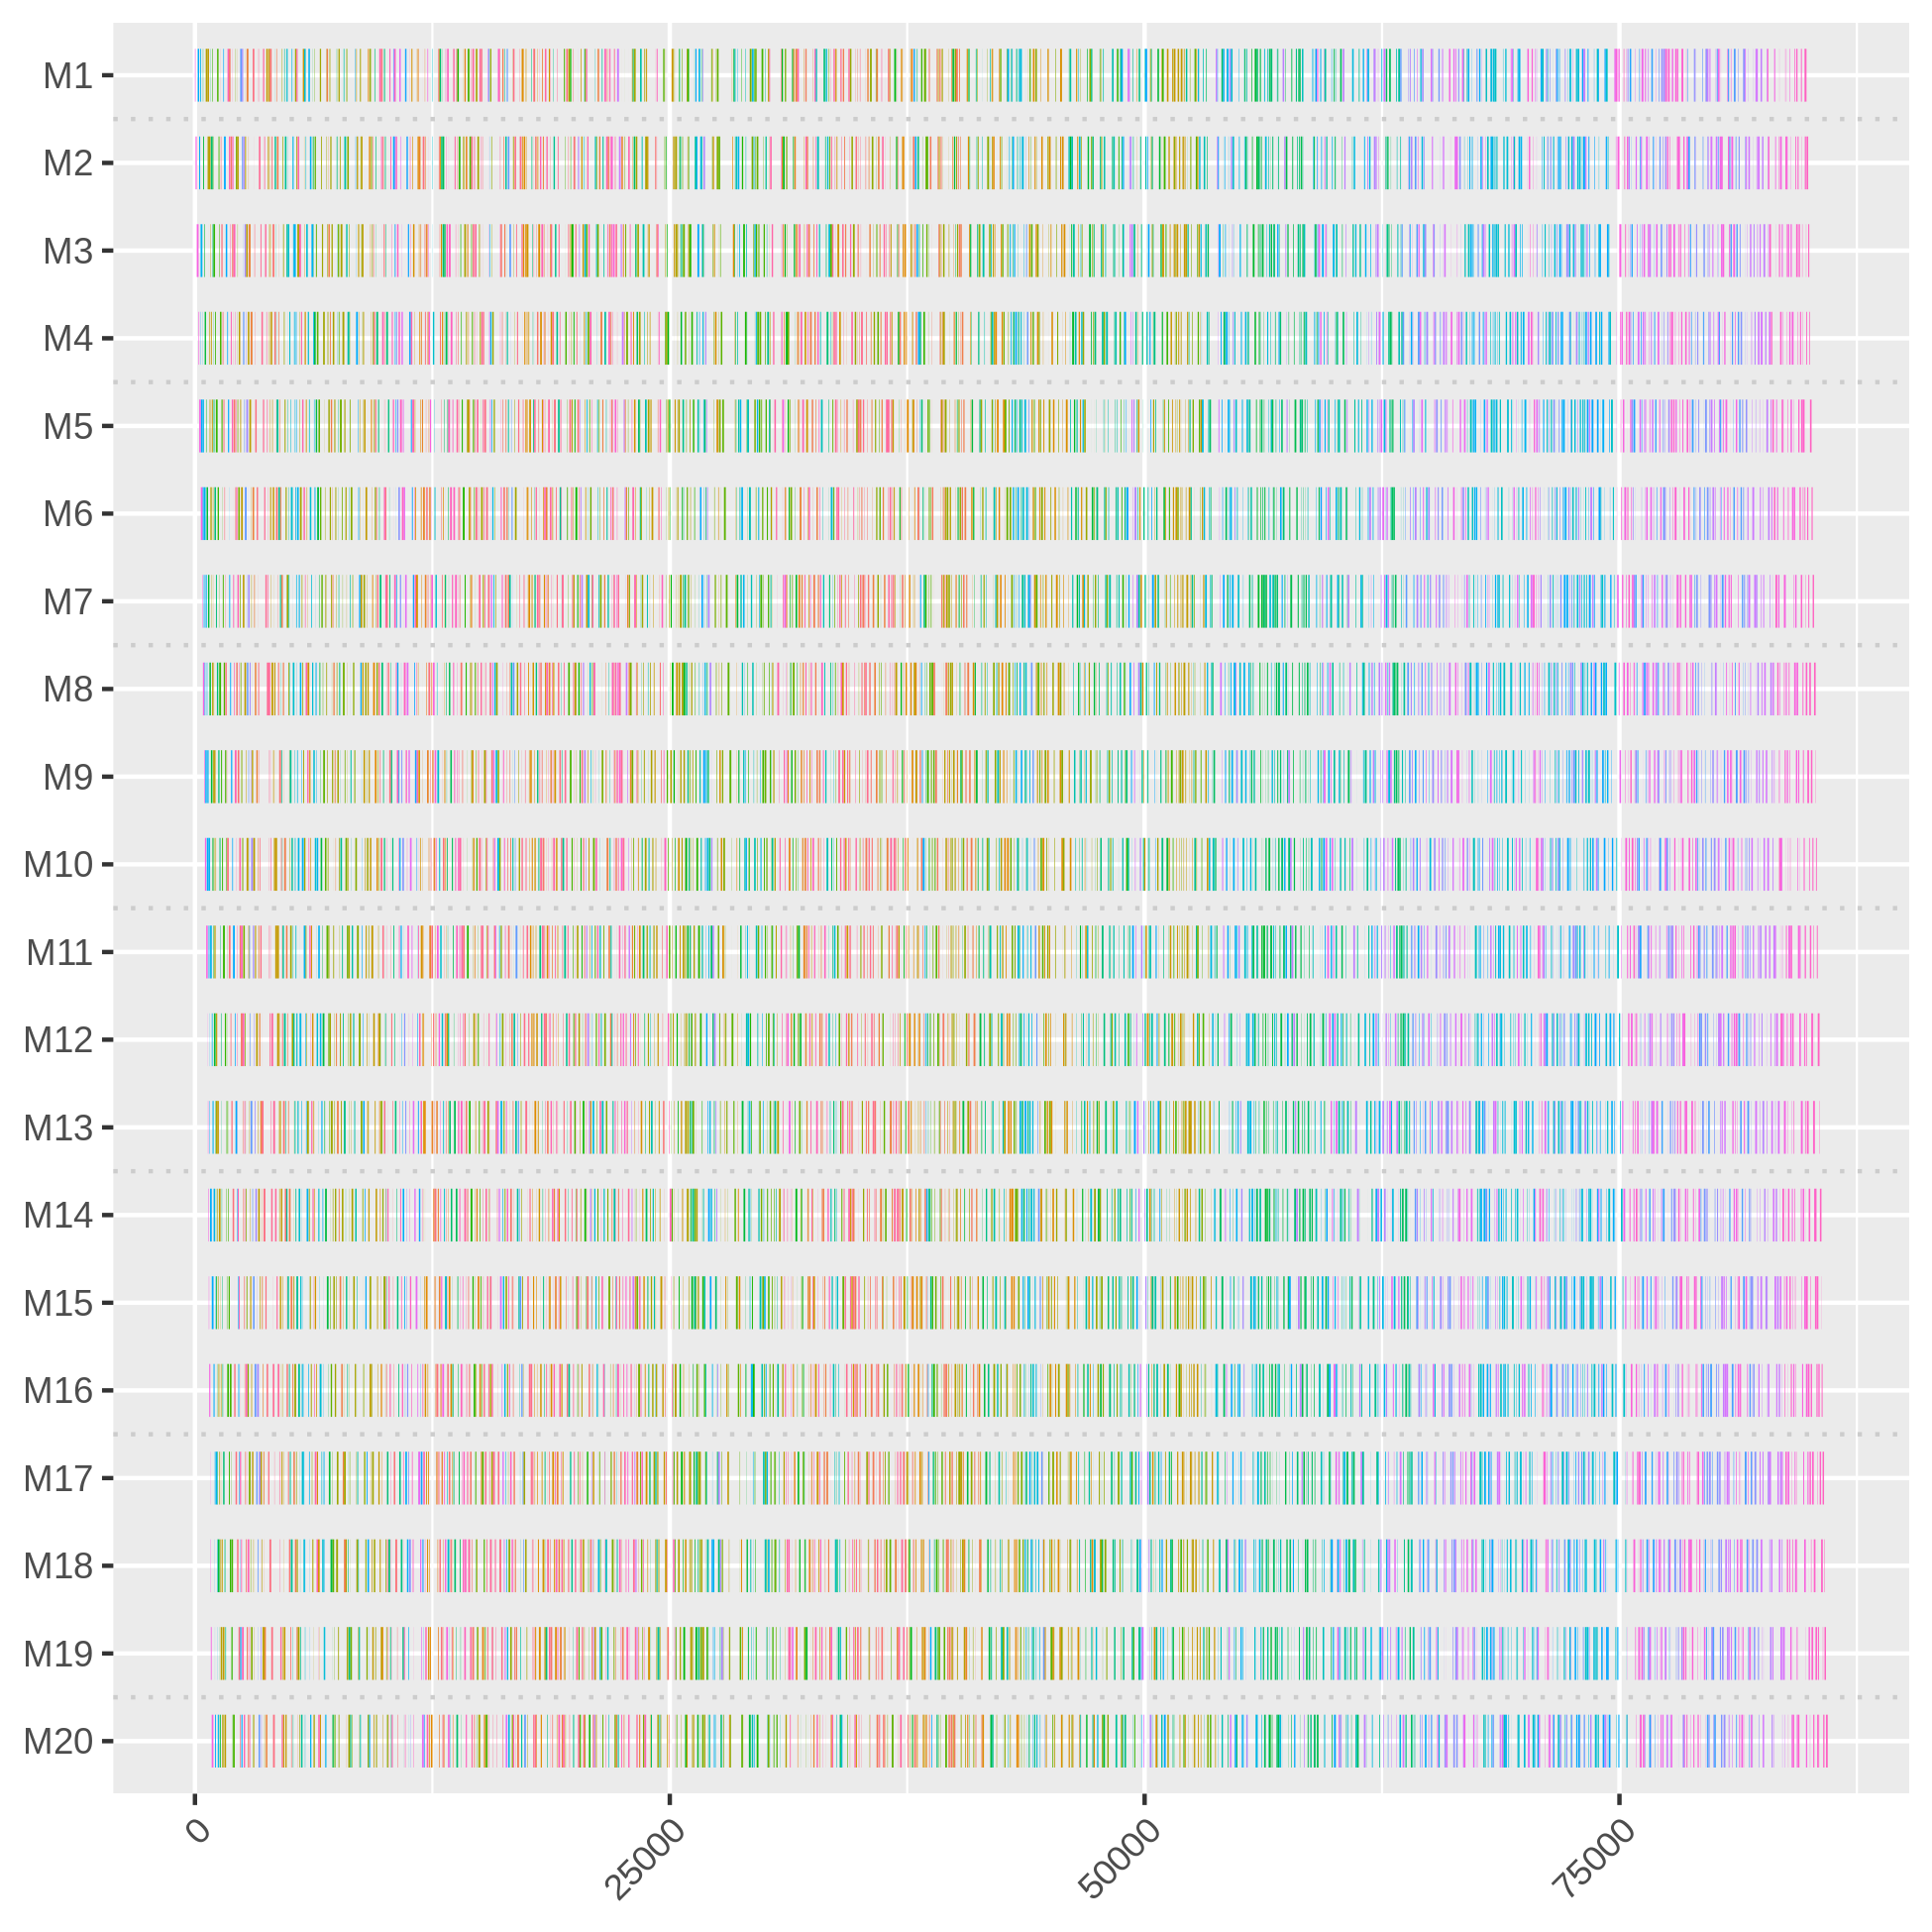
\includegraphics[width=\linewidth]{20_500_GC_3.png}
				\captionof{figure}{Gantt Chart for file 111.txt}
				
				\subsubsection{Results for Flow Shop Scheduling with No Wait}
					\newpage
				
					\begin{table}[ht]
						\scalebox{0.9}{
							\begin{tabular}{rlrr}
								\hline
								& {\textbf{File.name}} & {\textbf{Best.total.flow.time}} & {\textbf{\# func calls}} \\ 
								\hline
								{\textit{1}} & ../DataFiles/1.txt & 1614 & 567 \\ 
								{\textit{2}} & ../DataFiles/10.txt & 1494 & 562 \\ 
								{\textit{3}} & ../DataFiles/2.txt & 1644 & 565 \\ 
								{\textit{4}} & ../DataFiles/3.txt & 1581 & 566 \\ 
								{\textit{5}} & ../DataFiles/4.txt & 1676 & 564 \\ 
								{\textit{6}} & ../DataFiles/5.txt & 1585 & 566 \\ 
								{\textit{7}} & ../DataFiles/6.txt & 1577 & 565 \\ 
								{\textit{8}} & ../DataFiles/7.txt & 1548 & 564 \\ 
								{\textit{9}} & ../DataFiles/8.txt & 1634 & 561 \\ 
								{\textit{10}} & ../DataFiles/9.txt & 1649 & 570 \\ 
								{\textit{11}} & ../DataFiles/11.txt & 2339 & 570 \\ 
								{\textit{12}} & ../DataFiles/12.txt & 2286 & 566 \\ 
								{\textit{13}} & ../DataFiles/13.txt & 2089 & 566 \\ 
								{\textit{14}} & ../DataFiles/14.txt & 1997 & 566 \\ 
								{\textit{15}} & ../DataFiles/15.txt & 2249 & 570 \\ 
								{\textit{16}} & ../DataFiles/16.txt & 2146 & 566 \\ 
								{\textit{17}} & ../DataFiles/17.txt & 2206 & 569 \\ 
								{\textit{18}} & ../DataFiles/18.txt & 2223 & 562 \\ 
								{\textit{19}} & ../DataFiles/19.txt & 2147 & 570 \\ 
								{\textit{20}} & ../DataFiles/20.txt & 2140 & 566 \\ 
								{\textit{21}} & ../DataFiles/21.txt & 3224 & 567 \\ 
								{\textit{22}} & ../DataFiles/22.txt & 2990 & 565 \\ 
								{\textit{23}} & ../DataFiles/23.txt & 3235 & 570 \\ 
								{\textit{24}} & ../DataFiles/24.txt & 3270 & 568 \\ 
								{\textit{25}} & ../DataFiles/25.txt & 3231 & 570 \\ 
								{\textit{26}} & ../DataFiles/26.txt & 3218 & 569 \\ 
								{\textit{27}} & ../DataFiles/27.txt & 3267 & 567 \\ 
								{\textit{28}} & ../DataFiles/28.txt & 2978 & 568 \\ 
								{\textit{29}} & ../DataFiles/29.txt & 3260 & 568 \\ 
								{\textit{30}} & ../DataFiles/30.txt & 3218 & 568 \\ 
								{\textit{31}} & ../DataFiles/31.txt & 3639 & 3657 \\ 
								{\textit{32}} & ../DataFiles/32.txt & 3837 & 3662 \\ 
								{\textit{33}} & ../DataFiles/33.txt & 3625 & 3641 \\ 
								{\textit{34}} & ../DataFiles/34.txt & 3636 & 3616 \\ 
								{\textit{35}} & ../DataFiles/35.txt & 3727 & 3650 \\ 
								{\textit{36}} & ../DataFiles/36.txt & 3573 & 3661 \\ 
								{\textit{37}} & ../DataFiles/37.txt & 3542 & 3645 \\ 
								{\textit{38}} & ../DataFiles/38.txt & 3601 & 3658 \\ 
								{\textit{39}} & ../DataFiles/39.txt & 3472 & 3662 \\ 
								{\textit{40}} & ../DataFiles/40.txt & 3694 & 3639 \\ 
								{\textit{41}} & ../DataFiles/41.txt & 4727 & 3647 \\ 
								{\textit{42}} & ../DataFiles/42.txt & 4630 & 3657 \\ 
								{\textit{43}} & ../DataFiles/43.txt & 4736 & 3657 \\ 
								{\textit{44}} & ../DataFiles/44.txt & 4868 & 3659 \\ 
								{\textit{45}} & ../DataFiles/45.txt & 4874 & 3662 \\ 
								\hline
							\end{tabular}
						}
					\clearpage
					\end{table}
					
					\begin{table}[ht]
						\scalebox{0.9}{
							\begin{tabular}{rlrr}
								\hline
								& {\textbf{File.name}} & {\textbf{Best.total.flow.time}} & {\textbf{\# func calls}} \\ 
								\hline
								{\textit{1}} & ../DataFiles/46.txt & 4744 & 3658 \\ 
								{\textit{2}} & ../DataFiles/47.txt & 4901 & 3664 \\ 
								{\textit{3}} & ../DataFiles/48.txt & 4782 & 3663 \\ 
								{\textit{4}} & ../DataFiles/49.txt & 4705 & 3651 \\ 
								{\textit{5}} & ../DataFiles/50.txt & 4728 & 3663 \\ 
								{\textit{6}} & ../DataFiles/51.txt & 6828 & 3664 \\ 
								{\textit{7}} & ../DataFiles/52.txt & 6593 & 3661 \\ 
								{\textit{8}} & ../DataFiles/53.txt & 6590 & 3662 \\ 
								{\textit{9}} & ../DataFiles/54.txt & 6539 & 3667 \\ 
								{\textit{10}} & ../DataFiles/55.txt & 6642 & 3671 \\ 
								{\textit{11}} & ../DataFiles/56.txt & 6604 & 3665 \\ 
								{\textit{12}} & ../DataFiles/57.txt & 6655 & 3667 \\ 
								{\textit{13}} & ../DataFiles/58.txt & 6549 & 3668 \\ 
								{\textit{14}} & ../DataFiles/59.txt & 6692 & 3664 \\ 
								{\textit{15}} & ../DataFiles/60.txt & 6618 & 3664 \\ 
								{\textit{16}} & ../DataFiles/61.txt & 7328 & 14782 \\ 
								{\textit{17}} & ../DataFiles/62.txt & 7078 & 14785 \\ 
								{\textit{18}} & ../DataFiles/63.txt & 6850 & 14802 \\ 
								{\textit{19}} & ../DataFiles/64.txt & 6725 & 14788 \\ 
								{\textit{20}} & ../DataFiles/65.txt & 6879 & 14781 \\ 
								{\textit{21}} & ../DataFiles/66.txt & 6966 & 14797 \\ 
								{\textit{22}} & ../DataFiles/67.txt & 6976 & 14807 \\ 
								{\textit{23}} & ../DataFiles/68.txt & 6991 & 14813 \\ 
								{\textit{24}} & ../DataFiles/69.txt & 7242 & 14811 \\ 
								{\textit{25}} & ../DataFiles/70.txt & 7136 & 14802 \\ 
								{\textit{26}} & ../DataFiles/71.txt & 8949 & 14797 \\ 
								{\textit{27}} & ../DataFiles/72.txt & 8857 & 14817 \\ 
								{\textit{28}} & ../DataFiles/73.txt & 9170 & 14826 \\ 
								{\textit{29}} & ../DataFiles/74.txt & 9571 & 14808 \\ 
								{\textit{30}} & ../DataFiles/75.txt & 8982 & 14815 \\ 
								{\textit{31}} & ../DataFiles/76.txt & 8866 & 14821 \\ 
								{\textit{32}} & ../DataFiles/77.txt & 8869 & 14808 \\ 
								{\textit{33}} & ../DataFiles/78.txt & 8983 & 14792 \\ 
								{\textit{34}} & ../DataFiles/79.txt & 9277 & 14791 \\ 
								{\textit{35}} & ../DataFiles/80.txt & 9304 & 14826 \\ 
								{\textit{36}} & ../DataFiles/81.txt & 11927 & 14811 \\ 
								{\textit{37}} & ../DataFiles/82.txt & 12517 & 14780 \\ 
								{\textit{38}} & ../DataFiles/83.txt & 12077 & 14830 \\ 
								{\textit{39}} & ../DataFiles/84.txt & 12406 & 14715 \\ 
								{\textit{40}} & ../DataFiles/85.txt & 12102 & 14800 \\ 
								{\textit{41}} & ../DataFiles/86.txt & 12059 & 14812 \\ 
								{\textit{42}} & ../DataFiles/87.txt & 12339 & 14820 \\ 
								{\textit{43}} & ../DataFiles/88.txt & 12308 & 14802 \\ 
								{\textit{44}} & ../DataFiles/89.txt & 12163 & 14802 \\ 
								{\textit{45}} & ../DataFiles/90.txt & 12442 & 14719 \\ 
								{\textit{46}} & ../DataFiles/100.txt & 17519 & 59058 \\ 
								\hline
							\end{tabular}
						}
					\end{table}
					\clearpage
					
					\begin{table}[ht]
						
						\scalebox{0.9}{
							\begin{tabular}{rlrr}
								\hline
								& {\textbf{File.name}} & {\textbf{Best.total.flow.time}} & {\textbf{\# func calls}} \\ 
								\hline
								{\textit{1}} & ../DataFiles/91.txt & 17564 & 59189 \\ 
								{\textit{2}} & ../DataFiles/92.txt & 17628 & 59302 \\ 
								{\textit{3}} & ../DataFiles/93.txt & 17359 & 59187 \\ 
								{\textit{4}} & ../DataFiles/94.txt & 17692 & 59050 \\ 
								{\textit{5}} & ../DataFiles/95.txt & 17286 & 59357 \\ 
								{\textit{6}} & ../DataFiles/96.txt & 17595 & 59192 \\ 
								{\textit{7}} & ../DataFiles/97.txt & 17663 & 59317 \\ 
								{\textit{8}} & ../DataFiles/98.txt & 17637 & 59444 \\ 
								{\textit{9}} & ../DataFiles/99.txt & 17506 & 59137 \\ 
								{\textit{10}} & ../DataFiles/101.txt & 22958 & 59075 \\ 
								{\textit{11}} & ../DataFiles/102.txt & 23402 & 59198 \\ 
								{\textit{12}} & ../DataFiles/103.txt & 23207 & 59241 \\ 
								{\textit{13}} & ../DataFiles/104.txt & 23354 & 59225 \\ 
								{\textit{14}} & ../DataFiles/105.txt & 22958 & 59214 \\ 
								{\textit{15}} & ../DataFiles/106.txt & 23103 & 59333 \\ 
								{\textit{16}} & ../DataFiles/107.txt & 23099 & 59272 \\ 
								{\textit{17}} & ../DataFiles/108.txt & 23382 & 59291 \\ 
								{\textit{18}} & ../DataFiles/109.txt & 23084 & 59329 \\ 
								{\textit{19}} & ../DataFiles/110.txt & 22944 & 59354 \\ 
								{\textit{20}} & ../DataFiles/111.txt & 54322 & 371479 \\ 
								{\textit{21}} & ../DataFiles/112.txt & 55440 & 371041 \\ 
								{\textit{22}} & ../DataFiles/113.txt & 54803 & 370990 \\ 
								{\textit{23}} & ../DataFiles/114.txt & 54526 & 371147 \\ 
								{\textit{24}} & ../DataFiles/115.txt & 54944 & 371190 \\ 
								{\textit{25}} & ../DataFiles/116.txt & 55518 & 371742 \\ 
								{\textit{26}} & ../DataFiles/117.txt & 54347 & 371507 \\ 
								{\textit{27}} & ../DataFiles/118.txt & 54567 & 372950 \\ 
								{\textit{28}} & ../DataFiles/119.txt & 54161 & 372592 \\ 
								{\textit{29}} & ../DataFiles/120.txt & 55313 & 373286 \\ 
								\hline
							\end{tabular}
							
						}
						\caption{Results for Flow Shop Scheduling with No Wait}
					\end{table}
		
				\subsubsection{Analysis}
				As seen from table1 above, both the total flow time and the number of function calls increases as the number of machines or the number of jobs increases. Here results could not be compared to those on Taillard's website as the algorithm used to compute the total flow time is different. 
				
					
					
	\section{Conclusion}
			After implementing, experimenting with and analyzing the results of the NEH algorithm, it can be determined that even though NEH is reported to be the best algorithm for solving flow shop type of problems, its efficiency highly depends on how it is implemented. For example, the results of this project are different from those reported on Taillard's website even though the same concept was used to perform the optimization.
			
\end{document}